\documentclass[11pt,letterpaper]{article}
\usepackage[T1]{fontenc}
\usepackage[utf8]{inputenc}
\usepackage{lmodern}
\usepackage[margin=1in]{geometry}
\usepackage{amsmath,amssymb,amsthm,mathtools}
\usepackage{enumitem,booktabs,array,graphicx}
\usepackage{tikz,tikz-cd}
\usetikzlibrary{arrows.meta,positioning,fit}
\usepackage{microtype}
\usepackage{xcolor}
\definecolor{linkteal}{RGB}{0,83,91}
\usepackage{needspace}
\usepackage{xurl}
\usepackage[colorlinks=true,allcolors=linkteal]{hyperref}
\hypersetup{pdftitle={Conditional good minimal models for compact Kahler fourfolds},
 pdfauthor={OpenAI},pdflang={en-US},
 pdfsubject={Conditional nonvanishing and good minimal models for compact Kahler fourfolds}}
\newcommand{\Q}{\mathbb{Q}}
\newcommand{\R}{\mathbb{R}}
\newcommand{\C}{\mathbb{C}}
\newcommand{\Z}{\mathbb{Z}}
\newcommand{\PP}{\mathbb{P}}
\newcommand{\OO}{\mathcal{O}}
\newcommand{\cO}{\mathcal{O}}
\newcommand{\cF}{\mathcal{F}}
\newcommand{\cL}{\mathcal{L}}
\newcommand{\dd}{\mathrm{d}}
\newcommand{\ii}{\sqrt{-1}}
\newcommand{\ddc}{\mathrm{d}\mathrm{d}^{c}}
\newcommand{\NA}{\overline{\mathrm{NA}}}
\newcommand{\BC}{\mathrm{BC}}
\DeclareMathOperator{\Spec}{Spec}
\DeclareMathOperator{\Proj}{Proj}
\DeclareMathOperator{\Supp}{Supp}
\DeclareMathOperator{\Pic}{Pic}
\DeclareMathOperator{\Alb}{Alb}
\DeclareMathOperator{\Hom}{Hom}
\DeclareMathOperator{\rk}{rk}
\DeclareMathOperator{\codim}{codim}
\DeclareMathOperator{\mult}{mult}
\DeclareMathOperator{\ord}{ord}
\DeclareMathOperator{\vol}{vol}
\DeclareMathOperator{\im}{im}
\DeclareMathOperator{\Gr}{Gr}
\DeclareMathOperator{\DR}{DR}
\DeclareMathOperator{\id}{id}
\DeclareMathOperator{\tr}{tr}
\DeclareMathOperator{\Exc}{Exc}
\DeclareMathOperator{\NS}{NS}
\DeclareMathOperator{\divisor}{div}
\newtheorem{theorem}{Theorem}[section]
\newtheorem{proposition}[theorem]{Proposition}
\newtheorem{lemma}[theorem]{Lemma}
\newtheorem{corollary}[theorem]{Corollary}
\theoremstyle{definition}
\newtheorem{definition}[theorem]{Definition}
\newtheorem{assumption}[theorem]{Assumption}
\newtheorem{notation}[theorem]{Notation}
\theoremstyle{remark}
\newtheorem{remark}[theorem]{Remark}
\setlist{itemsep=3pt,topsep=5pt,leftmargin=*}
\allowdisplaybreaks[1]
\setlength{\emergencystretch}{2em}
\setcounter{tocdepth}{2}

\title{Conditional good minimal models\\for compact K\"ahler fourfolds}
\author{OpenAI}
\date{October 5, 2026}
\begin{document}
\maketitle
\begin{abstract}
Assuming orbifold Iitaka subadditivity, the specified pseudo-effective
fourfold minimal model program, and abundance for nef fourfold adjoints
of nonnegative Kodaira dimension, we prove the existence of good minimal
models for globally strongly \(\Q\)-factorial compact K\"ahler klt
fourfold pairs with effective rational boundary and analytically
pseudo-effective actual \(\Q\)-Cartier adjoint. The additional step
is nonvanishing. We prove it by
fibration arguments and, in algebraic dimension zero, by singular
metrics, holomorphic foliations, and extension from a reduced boundary.
The projective abundance argument used in the proof is included in full.
\end{abstract}
\tableofcontents
\newpage
\part{Compact K\"ahler fourfolds}
\section{Introduction}\label{sec:introduction}

The good minimal model problem asks whether a pseudo-effective
canonical adjoint can be made nef and generated by its sections on a
birational model. It joins two different questions: construction of a
minimal model and abundance of its nef adjoint. In the compact
K\"ahler category, the existence of the first pluricanonical section
is itself a substantial part of the problem. Positivity is analytic,
and even the passage from a cohomological identity to an identity of
holomorphic line bundles must be kept explicit.

The projective minimal model program provides the birational framework
\cite{BirationalGeometry,BCHM}. In dimension three the K\"ahler
theory has developed through nonvanishing, minimal models and
abundance \cite{DemaillyPeternellNonvanishing,HPMinimalModels,
CHPAbundance,CHPAbundanceErratum,GuenanciaPaunBogomolovGieseker}.
Work on fourfolds and on
pseudo-effective adjoints supplies further analytic and birational
tools \cite{DHPFourfoldMMP,HLLNonvanishing}. Our concern is the
precise additional nonvanishing argument needed when a
pseudo-effective fourfold MMP and abundance after nonvanishing are
available.

We make three explicit hypotheses, stated in
Section~\ref{sec:premises}: full orbifold Iitaka subadditivity in
Fujiki class \(\mathcal C\), the specified pseudo-effective klt
fourfold MMP conditional on that subadditivity, and abundance for nef
klt fourfold adjoints of nonnegative Kodaira dimension. Under these
premises we resolve positively the good-minimal-model assertion in
the following category.

\begin{theorem}[Conditional good minimal models]\label{thm:main}
Assume Assumptions~\ref{hyp:campana}, \ref{hyp:mmp}, and
\ref{hyp:effective-abundance}. Let \(X\) be a normal connected
compact K\"ahler fourfold, and let \(B\) be an effective rational
Weil divisor. Suppose that \((X,B)\) is klt, that its actual adjoint
\(D=K_X+B\) is \(\Q\)-Cartier and analytically
pseudo-effective, and that \(X\) is globally strongly
\(\Q\)-factorial in the sense of Definition~\ref{def:strong}.

Then there are a normal connected globally strongly
\(\Q\)-factorial compact K\"ahler fourfold \(Y\) and a
bimeromorphic map \(\phi:X\dashrightarrow Y\) such that:
\begin{enumerate}[label=\textup{(\roman*)}]
\item \(\phi\) extracts no prime divisor, and
      \(B_Y=\phi_*B\);
\item \((Y,B_Y)\) is klt and its actual adjoint
      \(D_Y=K_Y+B_Y\) is \(\Q\)-Cartier and analytically nef;
\item \(a(E;Y,B_Y)\ge a(E;X,B)\) for every prime divisor over
      the models, with strict inequality for each prime on \(X\)
      contracted by \(\phi\);
\item for some \(m>0\), the Cartier line bundle
      \(\OO_Y(mD_Y)\) is globally generated.
\end{enumerate}
\end{theorem}

The exponent may depend on the pair. Zero boundary, smooth fourfolds
and all numerical dimensions are included. Global strong
\(\Q\)-factoriality concerns all rank-one reflexive sheaves on
the whole space; it is not an assumption of local analytic
\(\Q\)-factoriality on every open subset. The conclusion concerns
the actual holomorphic adjoint line on the specified endpoint.

Assumption~\ref{hyp:mmp} already produces a nef minimal model with
properties~\textup{(i)}--\textup{(iii)}. The new conclusion needed
before Assumption~\ref{hyp:effective-abundance} can be applied is
the following.

\begin{theorem}[Nonvanishing on the nef endpoint]
\label{thm:nonvanishing}
Under Assumptions~\ref{hyp:campana}, \ref{hyp:mmp}, and
\ref{hyp:effective-abundance}, let \((Y,\Delta)\) be an ordinary
klt pair on a normal connected globally strongly
\(\Q\)-factorial compact K\"ahler fourfold. If \(\Delta\)
is effective and rational and the actual \(\Q\)-Cartier adjoint
\(J=K_Y+\Delta\) is analytically nef, then
\(\kappa(Y,J)\ge0\).
\end{theorem}

\subsection{Structure of the proof}

The projective case uses conditional projective log abundance. We
include its complete proof in
Appendices~\ref{proj:sec:introduction}--\ref{proj:sec:completion};
Lemma~\ref{red:log-iitaka} derives its precise logarithmic-Iitaka
premise from Assumption~\ref{hyp:campana}. Thus the projective
branch introduces no further conditional premise. For a
nonprojective endpoint, rational quotients, the Albanese map and
lower-dimensional nonvanishing reduce the problem to canonical
nonvanishing on a smooth non-uniruled fourfold, principally with
irregularity zero.

When algebraic dimension is positive, we first construct an actual
canonical pullback model over a projective base. The construction
uses sufficiently large ample twists, whose sections are already
known, and steps of a single empty-boundary program. Relative
rationality allows the twist to be chosen separately at each stage
without changing that program. The base has dimension at most three.
For a surface base, fiber powers convert subadditivity into the
intersection inequality needed for nonvanishing. For a threefold
base, the genus-one Hodge line and two modular forms give an
explicit crepant klt adjoint on the base. Their common divisorial
order is determined by one integrability calculation, including
exceptional base valuations.

The algebraic-dimension-zero argument has four parts.
\begin{enumerate}
\item A nef ordinary klt adjoint has a metric of minimal
singularities with zero Lelong numbers. The proof combines a
volume-normalized capacity estimate, a differentiated
Monge--Amp\`ere equation and a Bochner transport estimate. The
comparison at the end controls a concentrating residual measure
on the same sublevel set.
\item If the divisorial locus is empty and no signed canonical
frame exists, holomorphic forms produce a transverse spherical
structure. A fixed point on the full compact convex set of positive
currents and the compactification of its holonomy lead to a
contradiction with algebraic dimension zero.
\item Relative analytic constructions produce nef reduced-boundary
models while retaining actual line identities and the global
reflexive-sheaf condition. The required dlt special termination is
proved in the dimension order used by the construction.
\item Adjunction and gluing give a section on the \emph{whole}
reduced floor. In the nonprojective torsion case, the ambient
K\"ahler class controls the pluricanonical scalars around gluing
cycles. This extra structure is what makes the cycle argument
finite.
\end{enumerate}
Finally, finite divisorial support and hard Lefschetz with multiplier
ideals extend a high power of the floor section if ambient
nonvanishing were to fail. Two choices of reduced boundary, according
to whether a signed meromorphic pluricanonical tensor exists, finish
canonical nonvanishing. The result then returns to the original nef
endpoint of the stipulated MMP.

Several of these constructions have a scope beyond their immediate
use here: the metric lemma is dimension independent; the relative
descent argument treats global reflexive sheaves directly; the
genus-one calculation determines actual crepant orders; and the
floor argument isolates the role of a single ambient K\"ahler
class in nonprojective gluing. The long projective appendices are
organized separately so that the nonprojective argument can be read
with their precise theorem statement, while every new argument used
by that theorem remains available in the same manuscript.

Figure~\ref{fig:proof-map} records these uses and the return to the
original nef endpoint. In the projective appendices,
Assumption~\ref{proj:mmp:lower-models} is the lower-dimensional induction
hypothesis, discharged in Appendix~\ref{proj:sec:completion}.
\begin{figure}[!t]
\centering
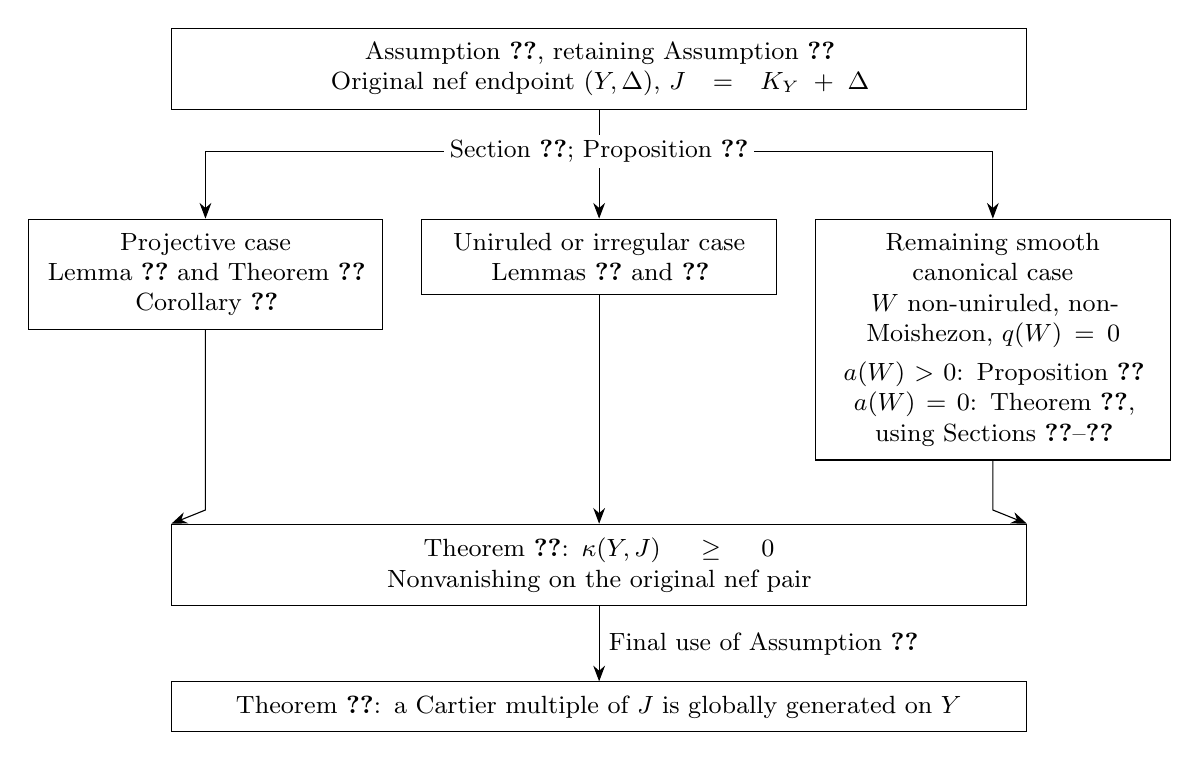
\begin{tikzpicture}[
  box/.style={draw,thin,align=center,font=\small,
    text width=4.15cm,inner sep=5pt},
  wide/.style={box,text width=10.5cm},
  flow/.style={-{Stealth[length=2mm]},thin}]
\node[wide] (endpoint) at (0,0)
  {Assumption~\ref{hyp:mmp}, retaining Assumption~\ref{hyp:campana}\\
   Original nef endpoint \((Y,\Delta)\), \(J=K_Y+\Delta\)};
\node[box,anchor=north] (projective) at (-5,-1.9)
  {Projective case\\
   Lemma~\ref{red:log-iitaka} and Theorem~\ref{proj:thm:main}\\
   Corollary~\ref{red:projective}};
\node[box,anchor=north] (direct) at (0,-1.9)
  {Uniruled or irregular case\\
   Lemmas~\ref{red:uniruled} and~\ref{red:irregular}};
\node[box,anchor=north] (canonical) at (5,-1.9)
  {Remaining smooth canonical case\\
   \(W\) non-uniruled, non-Moishezon, \(q(W)=0\)\par\smallskip
   \(a(W)>0\): Proposition~\ref{pos:nonvanishing}\\
   \(a(W)=0\): Theorem~\ref{end:canonical}, using Sections~\ref{met:section}--\ref{floor:sec}};
\node[wide] (nonvanishing) at (0,-6.3)
  {Theorem~\ref{thm:nonvanishing}: \(\kappa(Y,J)\geq0\)\\
   Nonvanishing on the original nef pair};
\node[wide] (good) at (0,-8.1)
  {Theorem~\ref{thm:main}: a Cartier multiple of \(J\)
   is globally generated on \(Y\)};
\draw[flow] (endpoint.south) -- (0,-1.05) -- (-5,-1.05) -- (projective.north);
\draw[flow] (0,-1.05) -- (direct.north);
\draw[flow] (0,-1.05) -- (5,-1.05) -- (canonical.north);
\node[fill=white,inner sep=2pt,font=\small] at (0,-1.05)
  {Section~\ref{red:section}; Proposition~\ref{red:reduction}};
\draw[flow] (projective.south) -- (-5,-5.6) -- (nonvanishing.north west);
\draw[flow] (direct.south) -- (nonvanishing.north);
\draw[flow] (canonical.south) -- (5,-5.6) -- (nonvanishing.north east);
\draw[flow] (nonvanishing.south) -- node[right,font=\small]
  {Final use of Assumption~\ref{hyp:effective-abundance}} (good.north);
\end{tikzpicture}
\caption{Reading map under Assumptions~\ref{hyp:campana}--\ref{hyp:effective-abundance}.
Lemma~\ref{red:log-iitaka} derives the sole premise of Theorem~\ref{proj:thm:main}
from Assumption~\ref{hyp:campana},
so the projective appendices add no independent conditional input.
The groupings indicate uses in this proof, not the full scope of the
component lemmas. Assumption~\ref{hyp:effective-abundance} also enters
intermediate constructions. All routes return nonvanishing to the
original nef pair before its final application on that endpoint.}
\label{fig:proof-map}
\end{figure}


\section{Conventions and the three hypotheses}\label{sec:premises}

All spaces are over \(\C\), unless a statement in the projective
appendices explicitly specifies another field of characteristic zero.
A compact K\"ahler space means a complex analytic space with a
K\"ahler form given by local smooth strictly plurisubharmonic potentials
on local embeddings. Our spaces are normal and connected, hence
irreducible. Smooth compact K\"ahler resolutions and resolutions of
meromorphic maps are obtained by projective modifications. We use the
usual resolution and K\"ahler modification theorems
\cite{HironakaResolution,VarouchasKahler}.

\subsection{Actual adjoints and positivity}

The canonical object on a normal space \(X\) is its reflexive canonical
sheaf \(\omega_X\). For an effective rational Weil divisor \(B\), the
notation \(D=K_X+B\) is an actual rational holomorphic line bundle
when, for some positive integer \(r\) clearing the coefficients of
\(B\),
\[
 L_r=\bigl(\omega_X^{[r]}\otimes\OO_X(rB)\bigr)^{**}
\]
is invertible. Its positive tensor powers define \(\OO_X(krD)\).
Here \(\omega_X^{[r]}=(\omega_X^{\otimes r})^{**}\), and divisorial
sheaves and their products are interpreted reflexively. An identity
\(D_1\sim_{\Q}D_2\) means an isomorphism of actual holomorphic line
bundles after a common positive integral multiple. Numerical equivalence
alone is never used to infer this identity.

Canonical divisor calculations can be performed with compatible local
canonical divisors on a common smooth model \(p:W\to X\). We use log
discrepancies
\begin{equation}\label{eq:discrepancy}
 a(E;X,B)=1+\operatorname{coeff}_E
       \bigl(K_W-p^*(K_X+B)\bigr).
\end{equation}
The pair is klt if these numbers are positive for every prime divisor
over \(X\), including primes on \(X\). In particular the boundary
coefficients are less than one. We do not assume at the outset that a
positive canonical power has a nonzero meromorphic section.

The adjoint \(D\) is \emph{analytically pseudo-effective} if
\(c_1(L_r)/r\) is represented by a closed positive \((1,1)\)-current
with local potentials. It is \emph{analytically nef} if this class is
in the closure of the K\"ahler cone in real Bott--Chern cohomology.
Equivalently, for a fixed K\"ahler form \(\omega\) and every
\(\varepsilon>0\), the line bundle has a smooth Hermitian metric
whose curvature, divided by \(r\), is bounded below by
\(-\varepsilon\omega\). On singular spaces the forms and potentials
are understood through local embeddings. Nonnegativity on compact
curves is a consequence of nefness, not its definition.

The Iitaka dimension \(\kappa(X,D)\) is \(-\infty\) if all positive
Cartier multiples have zero sections. Otherwise it is the maximum
dimension of the images of their complete linear systems. A rational
line bundle is \emph{semiample} if some positive Cartier multiple is
globally generated. In particular, a semiample rational line of Iitaka
dimension zero is torsion as an actual rational line bundle.
We write \(a(X)\) for algebraic dimension, and
\(q(M)=h^1(M,\OO_M)\) on smooth compact K\"ahler models.

\begin{definition}[Global strong \(\Q\)-factoriality]
\label{def:strong}
A normal compact space \(X\) is globally strongly
\(\Q\)-factorial if every coherent rank-one reflexive sheaf
\(\cF\) on the whole \(X\) has an invertible positive reflexive
power \(\cF^{[m]}=(\cF^{\otimes m})^{**}\).
\end{definition}

Definition~\ref{def:strong} is a condition on global sheaves. It does
not assert the same condition on every analytic open subset. Smooth
spaces satisfy it. The constructions below retain this global
condition when it is required; local analytic factoriality is not
inserted as an intermediate assumption.

\subsection{Orbifold subadditivity}

We give the model convention in the first hypothesis because the
distinction between the invariant base and the base on an arbitrary
model is used in the proof.

For a smooth compact space \(Z\) with an effective rational SNC
boundary \(\Gamma\) having coefficients in \([0,1]\), set
\[
 m_\Gamma(E)=
 \begin{cases}
 (1-\operatorname{coeff}_E\Gamma)^{-1},&
                  \operatorname{coeff}_E\Gamma<1,\\
 \infty,&\operatorname{coeff}_E\Gamma=1
 \end{cases}
\]
for every prime divisor \(E\). Thus the multiplicity off the boundary
is one; finite multiplicities need not be integers. If
\(g:(Z,\Gamma)\to S\) is a surjective morphism with connected
fibers and smooth base, put
\begin{equation}\label{eq:orbifold-base}
 \begin{split}
 m(g,\Gamma;P)&=
   \min_{E:\,g(E)=P}\bigl(\ord_E(g^*P)m_\Gamma(E)\bigr),\\
 B(g,\Gamma)&=\sum_P\left(1-\frac1{m(g,\Gamma;P)}\right)P.
 \end{split}
\end{equation}
Only divisors dominating \(P\) enter the minimum; the convention is
\(1/\infty=0\). The sum has finite support. This is the
inf-multiplicity convention.

An elementary equivalence of smooth source/base fibrations is a
commuting bimeromorphic diagram
\[
\begin{tikzcd}
 (Z',\Gamma')\arrow[r,"p"]\arrow[d,"g'"']&
 (Z,\Gamma)\arrow[d,"g"]\\
 S'\arrow[r,"q"]&S,
\end{tikzcd}
\]
where the maps are proper holomorphic modifications,
\(p_*\Gamma'=\Gamma\), and \(p\) is an orbifold morphism: for
every prime \(D\) on \(Z\) and every prime \(E\) on \(Z'\) with
\(t=\ord_E(p^*D)>0\),
\begin{equation}\label{eq:orbifold-morphism}
 t\,m_{\Gamma'}(E)\ge m_\Gamma(D).
\end{equation}
Infinite multiplicities are compared in the usual order, with
\(\infty\ge\infty\). All boundaries in these diagrams are rational
SNC boundaries in \([0,1]\). Equivalence is generated by these
diagrams with arrows allowed in either direction, not by arbitrary
boundary changes on a fixed space. Define
\begin{equation}\label{eq:orbifold-invariant}
 \kappa(g\mid\Gamma)=
 \inf_{g'\sim g}\kappa\bigl(S',K_{S'}+B(g',\Gamma')\bigr).
\end{equation}
For an initially normal possibly singular base, first resolve that
base and the main fiber product. On the resulting smooth source use
the strict transform of the original boundary plus the full reduced
exceptional divisor, and resolve the total support to SNC. These
modifications are isomorphisms over very general base points. The
invariant is independent of these choices.

A smooth-base fibration is \emph{neat} if there is a proper
bimeromorphic orbifold morphism of its source pair to a smooth pair,
with the boundary pushing forward, which contracts every source prime
mapping to codimension at least two in the given base. The hypothesis
below includes existence of suitable neat models and the formula
\begin{equation}\label{eq:neat-formula}
 \kappa(g\mid\Gamma)=\kappa\bigl(S,K_S+B(g,\Gamma)\bigr)
 \qquad\text{on a neat model}.
\end{equation}

\begin{assumption}[Full orbifold Iitaka subadditivity]
\label{hyp:campana}
Let \(X\) be a smooth compact connected manifold in Fujiki class
\(\mathcal C\), let \(\Delta\) be an effective rational SNC
boundary with coefficients in \([0,1]\), and let \(f:X\to Y\) be
a surjective holomorphic map with connected fibers onto a normal
compact irreducible complex space. In arbitrary dimensions,
\begin{equation}\label{eq:campana}
 \kappa(X,K_X+\Delta)\ge
 \kappa(F,K_F+\Delta|_F)+\kappa(f\mid\Delta),
\end{equation}
where \(F\) is a very general smooth fiber with SNC boundary
restriction, and the invariant base is defined by
\eqref{eq:orbifold-base}--\eqref{eq:neat-formula}.
\end{assumption}

Here very general means outside a countable union of proper closed
analytic subsets, as well as the critical values and unsuitable
boundary-stratum loci. The zero boundary is allowed, a point has
Kodaira dimension zero, and a sum with \(-\infty\) is
\(-\infty\). Neither source nor base need be projective. There is
no abundance, positivity or good-model premise in
Assumption~\ref{hyp:campana}. The displayed statement is the orbifold
subadditivity theorem of \cite[Theorem~1.1]{GrantCampana}. For later use,
on a smooth base the invariant
is at least \(\kappa(Y,K_Y)\), by effectivity of the orbifold
boundaries and smooth birational invariance.

\subsection{The pseudo-effective fourfold program}

The closed analytic cone \(\NA(X)\) consists of positive closed
bidimension-\((1,1)\) currents, modulo their pairings with all real
Bott--Chern \((1,1)\)-classes. We use its negative extremal rays in
the following hypothesis.

\begin{assumption}[Pseudo-effective fourfold MMP]
\label{hyp:mmp}
Assume Assumption~\ref{hyp:campana}. Start from an ordinary klt pair
\((X,B)\), where \(X\) is a normal irreducible globally strongly
\(\Q\)-factorial compact K\"ahler fourfold, \(B\) is effective
and rational, and the actual adjoint \(D=K_X+B\) is
\(\Q\)-Cartier and analytically pseudo-effective. No initial
modification is inserted. The following program exists and
terminates.

At every non-nef stage \((X_i,B_i)\) there is a nonzero
\(D_i\)-negative extremal ray of \(\NA(X_i)\), and every such
ray \(R\) may be chosen. It has a nef supporting class \(\alpha\)
with
\[
 \NA(X_i)\cap\alpha^\perp=R,
 \qquad \alpha-c_1(D_i)\text{ K\"ahler}.
\]
For every chosen ray there is a projective surjective bimeromorphic
contraction with connected fibers
\(f_i:X_i\to Z_i\), where \(Z_i\) is normal compact K\"ahler,
\(\rho_{\BC}(X_i/Z_i)=1\), and \(-D_i\) is relatively ample.
For some K\"ahler class \(\omega_i\) on \(Z_i\),
\[
 \NA(X_i)\cap(f_i^*\omega_i)^\perp=R.
\]
A divisorial contraction gives the next pair by pushforward. For a
small contraction the canonical log-canonical-positive flip is the
relative analytic Proj of
\[
 \bigoplus_{m\ge0}(f_i)_*\OO_{X_i}(mrD_i)
\]
for a sufficiently divisible positive Cartier index \(r\). This
algebra is locally finitely generated. Its Proj is normal and its
map to \(Z_i\) is projective, small and has connected fibers. The
boundary is strictly transformed; the new actual adjoint is
relatively ample, and its divisible Cartier multiple is the
tautological line bundle. Passing to a Veronese does not change the
model.

Each new pair is klt, compact K\"ahler and globally strongly
\(\Q\)-factorial, with \(\Q\)-Cartier analytically
pseudo-effective actual adjoint. Every nonterminal finite prefix
can be extended. Every program so obtained has finitely many steps,
irrespective of the choices of negative rays. It ends at an
analytically nef pair. The composite map extracts no prime and
satisfies the minimal-model discrepancy inequalities, weakly for
every prime over the models and strictly for every original prime
contracted.
\end{assumption}

Assumption~\ref{hyp:mmp} is supplied by
\cite[Theorem~6.20; Proposition~3.4 and its proof]{GrantMMP}
in the stated pseudo-effective subcase, without an orbifold Iitaka
hypothesis. The assumption gives neither a first plurisection
nor semiampleness. It includes no non-pseudo-effective program and
no dlt or generalized-pair extension. Fiber-type contractions are
not stopping outcomes in this program. The Cartier index may change
at every stage; no positive-side relative Bott--Chern dimension or
identification of absolute Bott--Chern spaces across a flip is
assumed. Trivial flops, inserted blowups and arbitrary birational
walks are not steps of the program. These distinctions matter when
auxiliary boundaries are used below.

\subsection{Abundance after nonvanishing}

\begin{assumption}[Effective fourfold abundance]
\label{hyp:effective-abundance}
Let \(X\) be a normal connected compact K\"ahler fourfold and
\(\Delta\) an effective rational boundary such that
\((X,\Delta)\) is klt and the actual adjoint
\(J=K_X+\Delta\) is \(\Q\)-Cartier. If \(J\) is analytically
nef and \(\kappa(X,J)\ge0\), then a positive Cartier multiple of
\(J\) is globally generated.
\end{assumption}

Assumption~\ref{hyp:effective-abundance} is the abundance-after-nonvanishing
theorem of \cite[Theorem~1.1]{GrantEffectiveAbundance}. It needs no strong
factoriality hypothesis and includes the actual torsion conclusion
when \(\kappa=0\). Its nonvanishing premise is explicit. No
auxiliary statement from its proof is granted separately.

The proof uses all three hypotheses. Apart from them, established
literature is invoked at its stated scope. The separate projective
abundance theorem used in the Moishezon branch is proved in
Appendices~\ref{proj:sec:introduction}--\ref{proj:sec:completion};
Lemma~\ref{red:log-iitaka} establishes its sole subadditivity premise
from Assumption~\ref{hyp:campana}.

\section{Reductions to canonical nonvanishing}
\label{red:section}

We first discharge the hypothesis of the projective theorem proved in
the appendices. We then reduce the remaining problem to canonical
nonvanishing on a smooth compact Kähler fourfold of irregularity zero.
Throughout, a fibration means a surjective holomorphic map with connected
fibers. Smooth source and target spaces do not mean that the map is
everywhere a submersion.

\subsection{The projective case}

\begin{lemma}[The logarithmic premise]\label{red:log-iitaka}
Assumption~\ref{hyp:campana} implies the following statement. Let
\(f:M\to S\) be a fibration between smooth connected complex projective
varieties, and let \(D_M,D_S\) be reduced effective simple normal crossing
divisors, possibly zero, such that
\begin{equation}\label{red:boundary-compatibility}
 \Supp(f^*D_S)\subseteq\Supp(D_M).
\end{equation}
For a very general smooth fiber \(F\), with \(D_F=D_M|_F\), one has
\begin{equation}\label{red:log-iitaka-inequality}
 \kappa(M,K_M+D_M)
 \geq \kappa(F,K_F+D_F)+\kappa(S,K_S+D_S).
\end{equation}
The usual convention for a \(-\infty\) summand applies.
\end{lemma}

\begin{proof}
It suffices to prove
\begin{equation}\label{red:invariant-base-bound}
 \kappa(f\mid D_M)\geq\kappa(S,K_S+D_S),
\end{equation}
because Assumption~\ref{hyp:campana} can then be applied to the original
pair \((M,D_M)\). We construct a neat model in the precise equivalence
class occurring in that assumption.

Flatten \(f\) by a projective modification of its base and resolve that
base, obtaining \(q:S'\to S\) with \(S'\) smooth projective. The main
strict transform before resolving the source can be taken
equidimensional over \(S'\). Indeed, start with the flat strict transform
provided by flattening and then base-change to the smooth resolved
base. Flatness persists; the unchanged smooth connected generic fiber
is irreducible, and flatness rules out vertical components. The main
space consequently has pure fibers of dimension \(\dim M-\dim S\).
Resolve it and its boundary to obtain a commuting diagram
\[
\begin{tikzcd}
 M' \arrow[r,"p"] \arrow[d,"f'"'] & M \arrow[d,"f"]\\
 S' \arrow[r,"q"'] & S .
\end{tikzcd}
\]
Here \(p\) is a projective birational morphism, \(M'\) is smooth
projective, and \(f'\) has connected fibers: its general fiber is
connected, so Stein factorization over the normal base \(S'\) has trivial
finite factor. Set \(D_{M'}\) equal to the strict transform of \(D_M\)
plus the full reduced \(p\)-exceptional divisor, and arrange that its
support is simple normal crossing.

This is an allowed orbifold modification of the source pair. It pushes
\(D_{M'}\) to \(D_M\). If a prime upstairs has positive pullback order
over a coefficient-one prime of \(D_M\), it is either that prime's
strict transform or a \(p\)-exceptional prime; in both cases its
coefficient upstairs is one. Thus the infinite-multiplicity condition
in the definition of an orbifold morphism is satisfied.

Moreover, \(p\) witnesses neatness. Let \(E\subset M'\) be a divisor
whose image in \(S'\) has codimension \(c\geq2\). In the equidimensional
main space its image has dimension at most
\[
 (\dim S-c)+(\dim M-\dim S)=\dim M-c.
\]
Its image in \(M\) therefore has codimension at least two, so \(E\) is
\(p\)-exceptional. Subsequent resolutions preserve this argument.

Let \(B_{f'}\) be the orbifold base divisor on \(S'\). Every component
of a pullback over a prime of
\((q^{-1}\Supp D_S)_{\mathrm{red}}\) belongs to \(D_{M'}\): this follows
from \eqref{red:boundary-compatibility} if it is not exceptional over
\(M\), and from the definition of \(D_{M'}\) otherwise. The multiplicity
assigned to each such source component is infinite. Consequently
\begin{equation}\label{red:orbifold-boundary-dominates}
 B_{f'}\geq(q^{-1}\Supp D_S)_{\mathrm{red}}.
\end{equation}
There is also an effective \(q\)-exceptional divisor \(E_S\) such that
\begin{equation}\label{red:log-base-comparison}
 K_{S'}+(q^{-1}\Supp D_S)_{\mathrm{red}}
   =q^*(K_S+D_S)+E_S
\end{equation}
for compatible canonical divisors. Above the boundary, this is the
nonnegativity of log discrepancies of the simple normal crossing pair
\((S,D_S)\); away from the boundary, it is the nonnegativity of the
ordinary discrepancies of the smooth space \(S\). Equivalently, a
blowup of a smooth center of codimension \(c\) contained in \(s\) boundary
components contributes \(c-s\) if the center lies in the boundary, and
\(c-1\) otherwise, both nonnegative.

The neat-model formula in Assumption~\ref{hyp:campana}, followed by
\eqref{red:orbifold-boundary-dominates} and
\eqref{red:log-base-comparison}, now gives
\[
 \kappa(f\mid D_M)
 =\kappa(S',K_{S'}+B_{f'})
 \geq\kappa(S,K_S+D_S).
\]
This proves \eqref{red:invariant-base-bound}. In particular, the infimum
in the definition of the invariant has been computed on an allowed neat
model, rather than replaced by the divisor of an arbitrary base model.
\end{proof}

\begin{corollary}[Projective abundance in the present setting]
\label{red:projective}
Under Assumption~\ref{hyp:campana}, a nef \(\Q\)-Cartier adjoint of a
normal projective log canonical pair over \(\C\), with effective rational
boundary, is semiample.
\end{corollary}

\begin{proof}
Lemma~\ref{red:log-iitaka} is exactly the logarithmic-Iitaka hypothesis
of Theorem~\ref{proj:conditional-log-abundance}. Apply that theorem,
whose full proof is included in the appendices.
\end{proof}

In particular, the Moishezon case of Theorem~\ref{thm:nonvanishing} is
settled. A compact Kähler Moishezon space with rational singularities is
projective by Namikawa's criterion \cite{NamikawaProjectivity}. Analytic klt
singularities are rational; this follows as well from relative vanishing
on a projective log resolution \cite{FujinoAnalyticMMP}. Thus a
Moishezon klt endpoint \((Y,\Delta)\) of
Assumption~\ref{hyp:mmp} is projective. Its rational analytic boundary
and adjoint are algebraic by Chow's theorem and GAGA, and analytic
nefness implies nonnegative degree on every curve. Corollary
\ref{red:projective} applies to its actual adjoint line.

\subsection{Lower-dimensional inputs and restriction to fibers}

We use smooth compact Kähler resolutions of spaces, pairs, and graphs.
The resolution and Kähler-modification theorems ensure that these can
be obtained by projective modifications and remain Kähler
\cite{HironakaResolution,VarouchasKahler}. A space in Fujiki class \(\mathcal C\)
has a smooth compact Kähler model. The quantities
\(\kappa(K_W)\), \(q(W)=h^0(W,\Omega_W^1)\), and \(a(W)\) for smooth
compact Kähler \(W\) are bimeromorphic invariants.

We recall precisely the lower-dimensional nonvanishing facts used
below. A smooth non-uniruled compact Kähler manifold of dimension at
most three has nonnegative canonical Kodaira dimension. In
nonprojective dimension three this is
\cite[Corollary~1.4]{HPMinimalModels}. More explicitly, take a terminal
minimal model by Höring--Peternell and apply canonical nonvanishing
\cite[Theorem~0.3]{DemaillyPeternellNonvanishing} to its nef canonical
class. Terminal discrepancy comparison pulls its plurisections back
to the smooth model.
In the projective case, the klt minimal model program and log abundance
in dimensions at most three imply nonvanishing for every effective
rational klt pair with pseudo-effective adjoint \cite{ThreefoldFlipsAbundance,KeelMatsukiMcKernan,KeelMatsukiMcKernanCorrection}.
Finally, Ou's Theorem~1.1 identifies non-uniruledness of a smooth compact
Kähler manifold with analytic pseudo-effectivity of its canonical class
\cite{OuUniruledness}. These inputs have no four-dimensional nonvanishing
conclusion.

We will repeatedly use the following elementary parameter observation.
Let \(f:Z\to S\) be a proper fibration between smooth compact complex
manifolds, and let a pseudo-effective rational adjoint on \(Z\) have a
closed positive representative with local potentials. Its restriction
to a smooth fiber is defined and positive for almost every parameter:
local plurisubharmonic potentials restrict unless they are identically
minus infinity, and Fubini excludes the latter event for almost every
parameter. This full-measure set meets the complement of any countable
union of proper analytic subsets. If the lower-dimensional results give
nonvanishing on those fibers, a fixed multiple has sections generically.
Indeed, on a connected smooth parameter open set the loci
\[
 \{s:h^0(Z_s,mL|_{Z_s})\geq1\},
\]
for divisible positive integers \(m\), are analytic jumping loci by
proper semicontinuity. If every one were proper, their union would have
measure zero. Some such locus is therefore the whole open set. Generic
base change gives a direct image of positive rank. The same reasoning
allows all required very-general smoothness and boundary conditions to
be imposed simultaneously.

\subsection{The uniruled and irregular cases}

\begin{lemma}[The uniruled reduction]\label{red:uniruled}
Assume Assumption~\ref{hyp:campana}.
Let \((Y,\Delta)\) be a non-Moishezon compact Kähler klt fourfold with
effective rational boundary and pseudo-effective \(\Q\)-Cartier adjoint
\(J=K_Y+\Delta\). If a smooth compact Kähler resolution of \(Y\) is
uniruled, then \(\kappa(Y,J)\geq0\).
\end{lemma}

\begin{proof}
Take the almost-holomorphic rational-chain quotient of a smooth
resolution \(W\) of \(Y\). Campana's rational quotient theorem in class
\(\mathcal C\) gives a quotient with base in that class and very general
fibers rationally connected after resolution
\cite[Theorem~2.6]{CampanaRationalQuotient}. Resolve the quotient and
the pair simultaneously to a fibration
\[
 f:W'\longrightarrow T,\qquad p:W'\longrightarrow Y,
\]
with \(W',T\) smooth compact Kähler. The very general fibers are
projective: rational-chain-connected manifolds in class \(\mathcal C\)
are Moishezon by Campana's algebraic connectedness criterion
\cite{CampanaAlgebraicConnectedness}, and a smooth Kähler Moishezon
manifold is projective. They are then rationally connected.

The quotient base is not uniruled; see also \cite[Lemma~8.10]{OuUniruledness}.
For completeness, suppose otherwise and choose a covering rational
curve through a very general point of \(T\). Pull the fibration back
to its normalization \(\PP^1\) and resolve the main component, obtaining
a smooth compact Kähler space \(Z\) over \(\PP^1\) with rationally
connected very general fiber. Such a fiber has no holomorphic one- or
two-forms. A global two-form on \(Z\) restricts to zero on those fibers;
the relative differential sequence over the smooth locus then places
it in the base-one-form times relative-one-form piece. Its restriction
there is again zero, so the two-form vanishes on a dense open and hence
everywhere. Thus \(H^0(Z,\Omega_Z^2)=0\). Rational approximation of a
Kähler class, followed by Kodaira's criterion, makes \(Z\) projective.
The Graber--Harris--Starr theorem supplies a section of
\(Z\to\PP^1\) \cite{GraberHarrisStarr}.

The chosen base point can be taken so that its original quotient fiber
is not contained in any of the countably many analytic exceptional
sets in the very-general quotient property. This follows from the
proper fiber-dimension theorem on the resolved quotient. Consequently
the rational curve is contained in none of the corresponding bad
parameter sets. Choose two distinct good parameters on it. In each
smooth projective rationally connected fiber, rational chains join a
very general point to the point of the section. The section joins
these two chains. Their projection to \(W\) is a rational chain joining
points of different very general rational-quotient fibers, where the
original almost-holomorphic quotient is defined. This contradicts the
quotient property. Hence \(T\) is not uniruled. Its dimension is
positive, since a point quotient would make \(W\) Moishezon, and is at
most three; the fiber dimension is likewise between one and three.

On the simultaneous log resolution write
\begin{equation}\label{red:klt-resolution}
 K_{W'}+\Gamma\sim_{\Q}p^*J+E,
 \qquad 0\leq\Gamma<1,\quad E\geq0,
\end{equation}
where \(\Gamma\) is simple normal crossing and \(E\) is
\(p\)-exceptional. Concretely, take the nonnegative part of the crepant
log pullback boundary; its negative part becomes \(E\).
The adjoint in \eqref{red:klt-resolution} is pseudo-effective. At a
very general smooth fiber \(F\) we can impose the klt simple normal
crossing restriction and also restrict its positive current, by the
parameter observation above. Projective nonvanishing in dimension at
most three gives \(\kappa(F,K_F+\Gamma|_F)\geq0\). The non-uniruled
base similarly satisfies \(\kappa(T,K_T)\geq0\).

For a smooth base, the invariant orbifold-base dimension is at least
its ordinary canonical Kodaira dimension: on every equivalent smooth
model the orbifold divisor is effective, and the smooth canonical
Kodaira dimension is birationally invariant. Assumption
\ref{hyp:campana} therefore gives
\(\kappa(W',K_{W'}+\Gamma)\geq0\). A resulting section pushes through
\eqref{red:klt-resolution} to a section of a positive multiple of
\(J\). The exceptional pole allowance disappears away from a
codimension-two subset of the normal target, and reflexive extension
fills that subset.
\end{proof}

\begin{lemma}[Irregular canonical nonvanishing]\label{red:irregular}
Assume Assumption~\ref{hyp:campana}. If \(W\) is a smooth non-uniruled
compact Kähler fourfold with \(q(W)>0\), then \(\kappa(W,K_W)\geq0\).
\end{lemma}

\begin{proof}
Resolve the Stein-factor base of the Albanese map and its main pullback.
This gives a fibration on smooth compact Kähler models, with a
positive-dimensional smooth base \(T\) mapping generically with full
rank to the Albanese torus. A suitable wedge of the invariant
one-forms on that torus pulls back to a nonzero section of \(K_T\).
The very general fiber has dimension at most three; if its dimension
is zero, it is a point. The pseudo-effective canonical class of the
total space restricts to the canonical class of almost every smooth
fiber. Lower-dimensional canonical nonvanishing and the parameter
observation supply \(\kappa(K_F)\geq0\) on very general fibers.
Assumption~\ref{hyp:campana}, with zero boundary, now gives canonical
nonvanishing on the resolved total space and hence on \(W\).
\end{proof}

\begin{proposition}[Canonical reduction]\label{red:reduction}
Under the three assumptions of the main theorem, it is enough for
Theorem~\ref{thm:nonvanishing} to prove canonical nonvanishing for every
smooth non-uniruled non-Moishezon compact Kähler fourfold \(W\) with
\(q(W)=0\).
\end{proposition}

\begin{proof}
Let \((Y,\Delta)\) be the nef klt endpoint in
Theorem~\ref{thm:nonvanishing}, and put \(J=K_Y+\Delta\). The
Moishezon case was settled by Corollary~\ref{red:projective}. Let
\(W\) be a smooth compact Kähler resolution in the remaining case.
If \(W\) is uniruled, Lemma~\ref{red:uniruled} applies. Otherwise
Ou's theorem makes \(K_W\) pseudo-effective. A section of a divisible
canonical power on \(W\) pushes to the corresponding reflexive
canonical power on \(Y\), and multiplication by the effective boundary
section, at a common multiple, gives a section of \(J\). Thus canonical
nonvanishing on \(W\) suffices. Lemma~\ref{red:irregular} handles
\(q(W)>0\), leaving exactly the stated case.

Once nonvanishing on this original endpoint is established,
Assumption~\ref{hyp:effective-abundance} makes its adjoint semiample.
Its other good-minimal-model and discrepancy properties have already
been supplied by Assumption~\ref{hyp:mmp}. None of the auxiliary
models constructed later needs to replace this endpoint.
\end{proof}

\section{Positive algebraic dimension}
\label{pos:section}

\begin{proposition}\label{pos:nonvanishing}
Assume Assumptions~\ref{hyp:campana}, \ref{hyp:mmp}, and
\ref{hyp:effective-abundance}. Let \(W\) be a smooth non-uniruled
compact Kähler fourfold with \(q(W)=0\) and \(0<a(W)<4\). Then
\(\kappa(W,K_W)\geq0\).
\end{proposition}

The first step constructs an actual canonical pullback over a
projective base. We then prove nonvanishing of that base line in each
of its three possible dimensions.

\subsection{A contraction index bound}

\begin{lemma}[A local rationality bound]\label{pos:rationality}
Let \((Z,\Delta)\) be an ordinary rational klt pair on a normal
\(n\)-dimensional compact Kähler space, with actual \(\Q\)-Cartier
adjoint \(J=K_Z+\Delta\). Let \(\pi:Z\to T\) be a projective
bimeromorphic morphism with connected fibers to a normal compact
Kähler space. Assume that \(-J\) is relatively ample and that all
contracted curves have class in one \(J\)-negative ray \(R\) of
\(\NA(Z)\). Let \(k>0\) be an integer such that \(kJ\) is Cartier,
and let \(L\) be a line bundle with \(L\cdot R>0\). For any
nontrivial fiber \(F\) of \(\pi\),
\begin{equation}\label{pos:index-bound}
 r_F:=\sup\{u:L+uJ\text{ has nonnegative degree on all curves of }F\}
 \geq\frac{1}{k(n+1)}.
\end{equation}
No local analytic \(\Q\)-factoriality is required.
In particular, this applies to the contractions in
Assumption~\ref{hyp:mmp}, with \(n=4\).
\end{lemma}

\begin{proof}
Every curve \(C\) in \(F\) has nonzero class, since a Kähler class
has positive degree on it, and its class belongs to \(R\). Therefore
\[
 r_F=\frac{L\cdot C}{-J\cdot C}>0
\]
is independent of \(C\). The restriction of \(L\) to the projective
fiber is numerically a positive multiple of the relatively ample
rational line \(-J\). It is thus ample on \(F\), and the openness of
fiberwise ampleness makes \(L\) relatively ample after shrinking around
the image point of \(F\).

Work over a small Stein neighborhood of that point, with compactum
equal to the point. At \(r_F\), the restriction of \(L+r_FJ\) is
numerically trivial, hence nef but not ample on the nontrivial fiber.
Fujino's relative rationality theorem applies to this finite positive
threshold: in lowest terms its denominator is at most
\(k(\dim F+1)\) \cite[Theorem~4.3.1]{FujinoAnalyticCone}. The
non-lc-locus condition is empty for a klt pair, and the singleton
compactum satisfies the required local condition on the Stein base.
The relative numerical space over it is finite dimensional, as is also
seen by restriction to the projective fiber. The theorem consequently
gives \(r_F\geq1/(k(\dim F+1))\), which implies
\eqref{pos:index-bound}.

The line-bundle formulation is expressly permitted by
\cite[Remark~4.3.4]{FujinoAnalyticCone}; the nearby ampleness assertion
is \cite[Lemma~2.2.4]{FujinoAnalyticCone}. Canonical divisors in that
theorem may be handled locally, in its formal canonical-class
convention. Alternatively, over the Stein neighborhood the proper
direct image of a rank-one canonical sheaf is coherent of rank one,
since the contraction is bimeromorphic. Cartan's theorem supplies a
generically nonzero section, hence a meromorphic canonical
representative there. This requires no global meromorphic canonical
frame on the compact source and no local \(\Q\)-factoriality. The
Cartier index used in the bound belongs to this stage alone.
\end{proof}

\subsection{An actual canonical pullback}

Put \(d=a(W)\). Resolve a map defined by \(d\) algebraically independent
meromorphic functions on \(W\). Stein factorization has a projective
base, since its finite map has projective image. Resolving that base
and the main graph, we may replace \(W\) by a smooth compact Kähler
model on which there is a fibration
\[
 b:W\longrightarrow S_0,
 \qquad S_0\text{ smooth connected projective},\quad\dim S_0=d.
\]
The generic fibers remain connected through these modifications; Stein
factorization over the normal resolved base gives connected fibers
everywhere. Fix a very ample line bundle \(H\) on \(S_0\).

Since \(K_W\) is pseudo-effective and \(4-d\leq3\), the restriction
and parameter argument in Section~\ref{red:section} gives
\(\rk b_*\OO_W(\ell K_W)>0\) for some positive integer \(\ell\).
Coherence and ample twisting on the projective base imply that
\(b_*\OO_W(\ell K_W)\otimes H^{\ell N}\) has a nonzero global
section for every sufficiently large integer \(N\). Thus there is
\(N_0\) such that
\begin{equation}\label{pos:all-large-twists}
 \kappa(K_W+Nb^*H)\geq0
 \qquad\text{for every integer }N\geq N_0.
\end{equation}

\begin{proposition}[The pullback model]\label{pos:pullback-model}
There are a canonical globally strongly \(\Q\)-factorial compact
Kähler fourfold \(V\), a normal projective variety \(T\) of dimension
\(d\), a fibration \(g:V\to T\), and an actual rational line bundle
\(A_T\in\Pic(T)\otimes\Q\), such that
\begin{equation}\label{pos:canonical-pullback}
 K_V\sim_{\Q}g^*A_T.
\end{equation}
The space \(V\) is obtained from the current smooth \(W\) by a finite
empty-boundary \(K\)-program allowed by Assumption~\ref{hyp:mmp}, and
\(K_V\) remains pseudo-effective.
\end{proposition}

\begin{proof}
At a stage \(V_i\) of the empty-boundary program that still maps to
\(S_0\), write \(b_i:V_i\to S_0\) and \(H_i=b_i^*H\).
All these stages are canonical. Indeed, a common projective resolution
of a negative canonical step gives the comparison
\begin{equation}\label{pos:canonical-step-comparison}
 p^*K_{\mathrm{before}}\sim_{\Q}q^*K_{\mathrm{after}}+G,
 \qquad G\geq0,
\end{equation}
with \(G\) exceptional over the after model. The comparison follows
from the projective analytic negativity lemma over the contraction
base: there is no extraction, and canonical negativity supplies the
relative sign. For flips both sides and their common resolution are
projective over that base. Compatible local canonical comparisons
glue to the intrinsic discrepancy divisor in
\eqref{pos:canonical-step-comparison}. Discrepancies therefore do not
decrease. Starting from smooth \(W\), this preserves canonicity. The
remaining category and pseudo-effectivity properties are part of
Assumption~\ref{hyp:mmp}.

Choose a Cartier index \(k_i\) for \(K_{V_i}\), and choose an integer
\begin{equation}\label{pos:stage-choice}
 N\geq N_0,\qquad N>5k_i.
\end{equation}
This choice is made anew at the current stage. The actual line
\(K_{V_i}+NH_i\) has an effective rational klt boundary representative:
take a general divisor in a sufficiently high free multiple of
\(NH_i\) and divide by that multiple. On a fixed log resolution the
system has no fixed exceptional component, and Bertini makes the
chosen member transverse to the exceptional strata; its small
coefficient preserves klt. Its adjoint is pseudo-effective because
\(K_{V_i}\) is pseudo-effective and \(H_i\) is semipositive.

If this adjoint is not analytically nef, Assumption~\ref{hyp:mmp}
supplies an extremal ray on which \(K_{V_i}+NH_i\) is negative.
Since \(H_i\) is the pullback of a semipositive form, the ray is also
\(K_{V_i}\)-negative. Take its contraction and its negative step for
the empty-boundary program. In fact
\begin{equation}\label{pos:base-line-zero-on-ray}
 H_i\cdot R_i=0.
\end{equation}
Otherwise Lemma~\ref{pos:rationality}, with \(L=H_i\) and
\(J=K_{V_i}\), gives
\[
 \frac{1}{5k_i}
 \leq\frac{H_i\cdot C}{-K_{V_i}\cdot C}
 <\frac1N
\]
on any curve of a nontrivial contraction fiber, contrary to
\eqref{pos:stage-choice}.

Every connected projective fiber of the contraction maps to a point
under \(b_i\). If its image had positive dimension, some curve in that
fiber would map nontrivially to the projective base and have positive
\(H_i\)-degree. Proper descent over the normal contraction target
therefore factors \(b_i\) through it. In a flip, composition with the
positive-side morphism gives \(b_{i+1}\). Thus the actual pullback line
\(H_i\), not merely its numerical class, continues to be the pullback
of the fixed \(H\).

Repeat this procedure as long as the selected twist is not nef.
Every step actually taken is a step of the single empty-boundary
\(K\)-program starting from \(W\). The changing integers \(N\)
select rays; they do not change that program's boundary. If the
procedure were infinite, it would contradict the arbitrary termination
assertion in Assumption~\ref{hyp:mmp}. It therefore reaches a stage
\(V_i\) at which its selected \(K_{V_i}+NH_i\) is nef. In particular,
if the canonical program reaches a nef canonical class, the selected
semipositive twist is nef there as well.

For this final value of \(N\), \eqref{pos:all-large-twists} already
gave a section on the original \(W\). Clear the finitely many Cartier
indices of the chosen program. Since no step extracts a prime and all
maps agree to \(S_0\), that section pushes through every step as a
section of the corresponding actual twisted canonical power.
Reflexive extension across codimension two on each normal target
justifies the pushforward. Hence
\(\kappa(K_{V_i}+NH_i)\geq0\) before abundance is invoked.
Assumption~\ref{hyp:effective-abundance}, applied to the klt
representative above, makes this actual line semiample.

Set \(V=V_i\), choose a free integral multiple
\(m(K_V+NH_i)\), and let \(h:V\to\PP^r\) be its morphism.
Take the Stein factorization \(g:V\to T\) of \((b_i,h)\).
The variety \(T\) is normal and finite over the projective image,
hence projective. Let \(a:T\to S_0\) and \(c:T\to\PP^r\) be the
induced maps. We have \(\dim T\geq d\) because \(a\) is surjective,
and \(\dim T\leq a(V)=d\) because \(T\) is projective. Define
\begin{equation}\label{pos:actual-base-line}
 A_T=\frac1m c^*\OO_{\PP^r}(1)-N a^*H
 \quad\text{in }\Pic(T)\otimes\Q.
\end{equation}
The defining evaluation isomorphism for \(h\) and the actual identity
\(H_i=g^*a^*H\) prove \eqref{pos:canonical-pullback}.
\end{proof}

Choose a smooth projective resolution \(\mu:S\to T\), and resolve
the main graph to obtain a smooth compact Kähler \(M\) with
\(p:M\to V\) and a fibration \(f:M\to S\). Put \(A=\mu^*A_T\).
Canonicity and the fixed actual isomorphism in
\eqref{pos:canonical-pullback} give
\begin{equation}\label{pos:resolved-pullback}
 K_M\sim_{\Q}f^*A+R,
 \qquad R\geq0\text{ and }R\text{ is }p\text{-exceptional}.
\end{equation}
This is an identity of rational line bundles; all further resolutions
use its canonical transform. Pullback of holomorphic one-forms gives
\(q(S)\leq q(M)=q(W)=0\).

The rational line \(A\) is pseudo-effective. To see this with the
analytic definition, pull a positive representative \(\Theta\) of
\(c_1(K_V)\), with local potentials, to \(M\). The map \(p\) is
dominant, so its plurisubharmonic potentials do not become identically
minus infinity. If \(\omega\) is a Kähler form on \(M\), then
\[
 f_*(p^*\Theta\wedge\omega^{4-d})
\]
is a closed positive \((1,1)\)-current. The projection formula puts its
class in \(v\,c_1(A)\), where the degree-zero closed current
\(f_*(\omega^{4-d})=v\) is the positive constant volume of a smooth
general fiber. Division by \(v\) proves the assertion. Since \(S\)
is projective, this also gives numerical divisor pseudo-effectivity
\cite{BDPP}.

It remains to prove \(\kappa(S,A)\geq0\). A section then pulls back
through \eqref{pos:resolved-pullback}, multiplied by the effective
exceptional section, to a canonical plurisection on \(M\), and hence
on \(W\). If \(d=1\), the smooth projective curve \(S\) has
\(q(S)=0\), so it is \(\PP^1\); a pseudo-effective rational line on
it has nonnegative degree and has a section at a divisible multiple.
The two remaining dimensions require more information from the
fibration.

\subsection{A surface base and fiber powers}

Assume \(d=2\). Fix a sufficiently divisible positive integer \(m_0\)
for \eqref{pos:resolved-pullback}. On very general smooth fibers one
has
\begin{equation}\label{pos:surface-fiber-rank}
 h^0(F,mK_F)=1\qquad(m>0,\ m_0\mid m).
\end{equation}
At least one section is supplied by the effective divisor \(R|_F\).
If for a fixed divisible \(m\) the generic dimension were at least
two, generic base change and ample twisting of
\(f_*\OO_M(mK_M)\) would give two sections whose ratio is nonconstant
on a general fiber. Together with meromorphic functions from the
two-dimensional projective base this would give algebraic dimension
at least three, contrary to \(a(M)=2\). The analytic jumping loci
for the countably many \(m\)'s can be excluded simultaneously, proving
\eqref{pos:surface-fiber-rank}.

\begin{lemma}[A base intersection inequality]\label{pos:surface-inequality}
There are nonnegative rational numbers \(c_P\), indexed by the
finitely many \(\mu\)-exceptional curves on \(S\), such that
\begin{equation}\label{pos:surface-intersection}
 \left(A-K_S+\sum_Pc_PP\right)\cdot H'\geq0
\end{equation}
for every ample divisor \(H'\) on \(S\).
\end{lemma}

\begin{proof}
Choose a dense open set of \(S\) over which \(f\) is smooth and the
generator supplied by \eqref{pos:resolved-pullback} is not identically
zero on any fiber. This requires deleting a proper analytic subset:
a horizontal divisor cannot contain a whole fiber over a divisor in
the base without being vertical, by the fiber-dimension theorem; the
remaining degeneracies are proper analytic images or jumping loci.
Include all \(\mu\)-exceptional curves among the finitely many
complementary curves.

For each such curve \(P\), fix a component \(D\) of \(f^*P\)
dominating \(P\), write
\[
 e=\ord_D(f^*P),\qquad h=\operatorname{coeff}_D R,
\]
and make these choices before choosing any ample test curve or fiber
power. If \(P\) is not exceptional over \(T\), take \(D\) with
\(h=0\). Indeed, over a general point of its image divisor in the
normal \(T\), a local equation pulls back under the holomorphic
\(g\) to a divisor on \(V\) dominating that base divisor. The strict
transform of one such component has zero coefficient in the
\(p\)-exceptional \(R\). For an exceptional \(P\), set
\begin{equation}\label{pos:exceptional-pole-allowance}
 c_P=h/e.
\end{equation}

Replace \(H'\) by a sufficiently large very ample multiple and choose
a smooth member \(C\) of genus at least one. It can be chosen
transverse to all complementary curves at their general points,
avoiding their finitely many excluded points and any isolated bad
base points. Moreover, \(M_C=f^{-1}(C)\) is smooth by Bertini for
the pulled-back free system, and connected because \(f\) has connected
fibers. To retain \eqref{pos:surface-fiber-rank}, choose \(C\) through
one parameter where all those countably many equalities hold. A high
enough linear system through that point is free away from it; on its
fiber \(f\) is a submersion, so the same Bertini conclusion holds
there. Each jumping locus then cuts a proper analytic subset of
\(C\). Thus very general fibers of \(f_C:M_C\to C\) satisfy all
the equalities in \eqref{pos:surface-fiber-rank}.

By adjunction,
\begin{equation}\label{pos:curve-relative-canonical}
 K_{M_C/C}\sim_{\Q} f_C^*((A-K_S)|_C)+R_C,
 \qquad R_C=R|_{M_C}\geq0.
\end{equation}
At each \(z\in C\cap P\), a general point of the chosen component
\(D\) over \(z\) admits coordinates \((x,y_1,y_2)\) on \(M_C\)
and a parameter \(t\) on \(C\) in which
\begin{equation}\label{pos:surface-local-chart}
 t=x^e,\qquad R_C=h\{x=0\}
\end{equation}
in that chart. A unit in the pullback equation is absorbed into \(x\).
Such charts exist over general points of \(P\): the map \(D\to P\)
is generically submersive, and its intersections with the other
divisorial supports have smaller generic fiber dimension. Properness
and the fiber-dimension theorem allow the exceptional base points to
be discarded before \(C\) is chosen. These choices are independent of
the next integer \(r\).

For \(r\geq1\), take the main component of the \(r\)-fold fiber
product of \(M_C\) over \(C\), and a smooth compact Kähler resolution
\(Z_r\) of it. Over the good open set this fiber product is smooth
with connected fibers \(F^r\), hence has a unique main component.
It is an analytic subspace of a product of compact Kähler spaces;
the required Kähler resolution and connected-fiber morphism to \(C\)
follow as above. The general fiber has a canonical section by
\eqref{pos:surface-fiber-rank}, and \(\kappa(C)\geq0\).
Assumption~\ref{hyp:campana}, with zero boundary and in dimension
\(2r+1\), gives a nonzero section of \(mK_{Z_r}\) for some \(m>0\).
By taking a power, make \(m\) divisible by \(m_0\) and all indices
in use. It may depend on \(r\) and \(C\).

Over good parameters, the product formula and
\eqref{pos:surface-fiber-rank} make the fiberwise pluriform space
one-dimensional. The chosen section is therefore the product of the
\(r\) relative generators in
\eqref{pos:curve-relative-canonical}, times a base pluriform and a
scalar base coefficient. This coefficient is a section on the good
open of the line
\begin{equation}\label{pos:fiber-power-coefficient-line}
 \OO_C\bigl(m(K_C+r(A-K_S)|_C)\bigr).
\end{equation}
Indeed, its quotient by the displayed product is constant on very
general fibers; local submersion sections and analytic continuation
give meromorphic descent to that open. Evaluation at points where the
product does not vanish identically on the fiber makes the descended
coefficient holomorphic there.

We compute its order at a missing point \(z\). In
\eqref{pos:surface-local-chart}, a frame of
\(\OO_C(m(A-K_S)|_C)\) maps, up to a unit, to
\[
 x^{mh}\left(\frac{dx\wedge dy_1\wedge dy_2}{dt}\right)^{\!m}.
\]
On a normalization branch of the local \(r\)-fold product we have
\(x_1=x\), \(x_j=\zeta_jx\), where \(\zeta_j^e=1\). Multiplying
the \(r\) relative factors by one base factor \((dt)^m\), and using
\(dt=ex^{e-1}dx\), gives order
\begin{equation}\label{pos:fiber-power-order}
 m\bigl(rh-(r-1)(e-1)\bigr)
\end{equation}
along \(x=0\). This smooth normalization branch belongs to the main
component, being a closure of points with \(t\ne0\). The global
pluriform on \(Z_r\) has no pole at its generic divisor, by birational
comparison. Its scalar coefficient \(u\), pulled back by \(t=x^e\),
therefore extends meromorphically, with
\[
 e\,\ord_z(u)+m\bigl(rh-(r-1)(e-1)\bigr)\geq0.
\]
In particular,
\begin{equation}\label{pos:fiber-power-pole-bound}
 \ord_z(u)\geq-\frac{mrh}{e}.
\end{equation}
There is no pole allowance at a nonexceptional base curve, where
\(h=0\). The exceptional allowances are exactly
\(mr c_P\), with the fixed \(c_P\) in
\eqref{pos:exceptional-pole-allowance}.

The nonzero meromorphic coefficient in
\eqref{pos:fiber-power-coefficient-line}, with these pole bounds,
implies
\[
 \deg K_C+r\left(A-K_S+\sum_Pc_PP\right)\cdot C\geq0.
\]
Divide by \(r\) and let \(r\to\infty\), keeping \(C\) fixed.
Since \(C\) is a positive multiple of \(H'\), this proves
\eqref{pos:surface-intersection}.
\end{proof}

Take the surface Zariski decomposition \cite{BHPV}
\begin{equation}\label{pos:zariski-decomposition}
 A=P_0+N_0,
\end{equation}
where \(P_0\) is nef, \(N_0\geq0\) has negative-definite support
if nonzero, and \(P_0\) is orthogonal to every component of \(N_0\).
The negative-part linear equations give rational coefficients, so
\(P_0=A-N_0\) remains an actual rational line. For a
\(\mu\)-exceptional curve \(P\), \(A\cdot P=0\). If \(P\) belongs
to \(\Supp N_0\), orthogonality gives \(P_0\cdot P=0\); otherwise
both \(P_0\cdot P\) and \(N_0\cdot P\) are nonnegative, and their
sum is zero. Hence every such \(P\) is orthogonal to \(P_0\).

If \(P_0\equiv0\), the equality \(q(S)=0\) makes a divisible
multiple of \(P_0\) torsion, so \(P_0\) is zero in
\(\Pic(S)\otimes\Q\). If \(P_0^2>0\), the nef line \(P_0\) is
big. Either case supplies sections of a positive multiple of \(A\).
In the remaining case, \(P_0\not\equiv0\) and \(P_0^2=0\).
Test \eqref{pos:surface-intersection} on ample classes approaching
\(P_0\). The exceptional terms and \(A\cdot P_0\) vanish, giving
\(K_S\cdot P_0\leq0\). For large divisible \(\ell\),
\begin{equation}\label{pos:surface-riemann-roch}
 \chi(S,\ell P_0)
 =\chi(\OO_S)-\frac{\ell}{2}K_S\cdot P_0>0,
\end{equation}
since \(\chi(\OO_S)=1+h^{2,0}(S)>0\). Serre duality gives
\(H^2(S,\ell P_0)=0\) for large \(\ell\): the divisor
\(K_S-\ell P_0\) has negative degree against a fixed ample divisor.
Thus \(h^0(S,\ell P_0)>0\); multiplication by the section of
\(\ell N_0\) proves \(\kappa(S,A)\geq0\).

\subsection{A threefold base and genus-one orders}

Assume \(d=3\). The general fibers of \(g:V\to T\) are smooth
connected genus-one curves. Indeed, the singular locus of normal
\(V\) has dimension at most two, so misses a general fiber; generic
smoothness then applies, and \eqref{pos:canonical-pullback} makes its
canonical line torsion. Also all components of \(R\) in
\eqref{pos:resolved-pullback} are vertical over \(S\): their images
on \(V\) have dimension at most two.

Choose one integer \(m>0\), divisible by \(12\), that clears the
Cartier data and the actual isomorphism in
\eqref{pos:canonical-pullback}. It clears
\eqref{pos:resolved-pullback} on every smooth model subsequently
used. In fact, the pullback of a local frame of the Cartier line
\(\OO_V(mK_V)\), regarded on the regular locus as an
\(m\)-pluriform, has integral orders on every resolution. Those
orders are precisely \(m\operatorname{coeff}_E R\). There is thus
no need to choose a new index after a base blowup.

\subsubsection{The actual Hodge line and its growth}

Shrink to a dense open \(U\subset T_{\mathrm{reg}}\), also viewed
on \(S\), on which the family is smooth and agrees with its resolution.
Let \(\mathcal H\) be its line of holomorphic fiberwise one-forms.
It is a holomorphic line by Grauert base change; periods against local
integral cycles are holomorphic. Give it the Hodge norm, so that
\(\|\alpha\|^2\) is, up to a fixed convention, the fiber integral
of \(\ii\alpha\wedge\overline\alpha\).

Evaluation \(f^*\mathcal H\to\omega_{M/U}\) is an isomorphism:
a nonzero holomorphic one-form on a smooth genus-one curve has no zero.
Its \(m\)-th power, together with the fixed actual pullback identity,
gives an isomorphism of pullbacks of lines on \(U\). Applying
\(f_*\) and \(f_*\OO_M=\OO_U\) yields the actual identification
\begin{equation}\label{pos:actual-hodge-line}
 \mathcal H^{\otimes m}\simeq\mathcal L_m|_U,
 \qquad\mathcal L_m=\OO_S\bigl(m(A-K_S)\bigr).
\end{equation}
It is compatible on all birational base models over their common
open. No section of the genus-one fibration is needed: its first
integral cohomology, periods, and invariant differentials are defined
without an origin. In particular, \eqref{pos:actual-hodge-line}
leaves no unspecified flat line factor.

Let \(E_4\) and \(\Delta_{\mathrm{mod}}\) be the classical modular
forms of weights four and twelve for \(\mathrm{SL}_2(\Z)\)
\cite[Chapter~VII]{SerreArithmetic}. A local symplectic period basis
gives a parameter \(\tau\) in the upper half-plane and a normalized
Hodge frame with periods \(1,\tau\). The weight transformation laws
compensate the frame transformation, so these forms define sections
of \(\mathcal H^4\) and \(\mathcal H^{12}\). Define sections of
\(\mathcal L_m|_U\) by
\begin{equation}\label{pos:modular-sections}
 e_1=E_4^{m/4},\qquad e_2=\Delta_{\mathrm{mod}}^{m/12},
\end{equation}
where the tensor powers of the normalized frame are understood.

Near a general point of a complementary prime divisor on any smooth
base model, let \(t=0\) be its equation. There are positive constants
\(c,C,b\), locally uniform in the remaining coordinates, such that
\begin{equation}\label{pos:modular-growth}
 c\leq\bigl(\|e_1\|+\|e_2\|\bigr)^{2/m}
 \leq C(1+|\log|t||)^b\qquad(t\ne0).
\end{equation}
Here is the full growth argument. In the standard fundamental domain
the normalized frame has squared norm proportional to
\(\operatorname{Im}\tau\). Both scalar modular forms are bounded
there, \(\Delta_{\mathrm{mod}}\) has no zero in the upper half-plane,
and \(E_4\to1\) at the cusp. On the compact part their joint norm has
a positive minimum; at the cusp the \(E_4\) term supplies the same
positive lower bound. This also covers the case where \(e_1\) is
identically zero on the given family.

For the upper bound, restrict to punctured disks transverse to the
prime, with the other parameters in a small compact set and with
\(t\ne0\) inside \(U\). Lift the period map to universal covers.
Schwarz--Pick makes it distance-decreasing for the hyperbolic metrics.
The radial hyperbolic distance in a punctured disk, from a fixed
radius to \(|t|\), is
\(O(1)+O(\log|\log|t||)\). Starting period representatives at that
radius can be chosen in a bounded part of the fundamental domain,
uniformly in angle and the other parameters, by compactness inside
the smooth locus. Since \(\log\operatorname{Im}\tau\) changes by
at most hyperbolic distance, both \(\operatorname{Im}\tau\) and its
inverse are bounded by powers of \(1+|\log|t||\) along the lifted
radial paths. Returning to the fundamental domain preserves such a
bound, because for \(\gamma\in\mathrm{SL}_2(\Z)\),
\[
 \operatorname{Im}(\gamma\tau)
 \leq\max\{\operatorname{Im}\tau,(\operatorname{Im}\tau)^{-1}\}.
\]
The bounded scalar modular forms and the Hodge-frame norm now prove
the upper inequality in \eqref{pos:modular-growth}.

\subsubsection{The integration threshold and meromorphic extension}

Fix a prime \(P\subset S\), a local parameter \(t\) at its general
point, and a frame \(s\) of \(\mathcal L_m\). On a simultaneous log
resolution of \(R\) and \(f^*P\), recompute \(R\) by the canonical
comparison in \eqref{pos:resolved-pullback}. Define
\begin{equation}\label{pos:threshold-definition}
 t_P=\min_{E\mapsto P}
 \frac{1+\operatorname{coeff}_E R}{\ord_E(f^*P)}.
\end{equation}
The minimum is taken over components above the general point of
\(P\). It is positive because \(R\geq0\).

\begin{lemma}[The divisorial order identity]\label{pos:order-identity}
The sections \(e_1,e_2\) extend meromorphically to \(S\). If
\[
 \ell_P=\min_i\ord_P(e_i/s),
\]
omitting an identically zero section, then
\begin{equation}\label{pos:modular-order}
 \frac{\ell_P}{m}=1-t_P.
\end{equation}
The same identity holds on every subsequent smooth base model, using
its actual line \(\OO(m(A-K_S))\) and the fixed integer \(m\).
\end{lemma}

\begin{proof}
First identify the weighted integrability threshold of the frame:
\begin{equation}\label{pos:integrability-threshold}
 t_P=\sup\left\{u\in\R:
 |t|^{-2u}\|s\|^{2/m}\text{ is locally integrable near general }P
 \right\}.
\end{equation}
Multiply \(s\) by a local \(m\)-canonical base frame. Under
\eqref{pos:resolved-pullback}, the resulting total-space
pluriform has divisor \(mR\). On a smooth good fiber it is the
\(m\)-th tensor of a one-form, up to a scalar, so integrating its
\(2/m\)-density along the fiber gives \(\|s\|^{2/m}\) times the
smooth base coordinate density. Fubini and change of variables
therefore identify the weighted base integral with the total-space
integral. In simple normal crossing coordinates the latter has, at
a component \(E\), a factor
\[
 |x_E|^{2(h_E-u e_E)},\qquad
 h_E=\operatorname{coeff}_E R,\quad e_E=\ord_E(f^*P).
\]
Such a factor is integrable exactly when \(h_E-u e_E>-1\).
Choose the point of \(P\) generally to exclude components not
dominating it, and use properness for a finite covering of its inverse
image. The conditions are exactly those in
\eqref{pos:threshold-definition}, proving
\eqref{pos:integrability-threshold}.

We next establish a polynomial lower bound on the Hodge norm of
\(s\), without assuming meromorphic extension of the modular
coefficients. Choose one component \(E\) above general \(P\), of
multiplicity \(e\) and coefficient \(h\) in \(R\). At a general
point of \(E\), the map has local coordinates
\[
 (t,z_1,z_2)=(x^e,z_1,z_2)
\]
on the base, with one further fiber coordinate \(y\) on the source.
The map \(E\to P\) is submersive there, units have been absorbed
into \(x\), and no other divisorial support meets the chart. The
total pluriform associated with \(s\) is a unit times
\(x^{mh}(dx\wedge dz_1\wedge dz_2\wedge dy)^m\).
After division by the base pluriform, its relative coefficient is
a unit times \(x^{m(h-e+1)}\). Integrating on a fixed smaller disk
in the \(y\)-coordinate gives
\begin{equation}\label{pos:polynomial-lower-bound}
 \|s\|^{2/m}\geq c\,|t|^{2(h-e+1)/e}.
\end{equation}
These charts are available above every point of \(P\) outside a
proper analytic subset. Indeed, the non-submersive locus and
intersections with the removed supports are proper subsets of \(E\);
those that dominate \(P\) have strictly smaller generic fiber
dimension. Properness and the fiber-dimension theorem show that a
general fiber of \(E\to P\) is not exhausted by them. We also omit
the singular and intersection loci of complementary base divisors.

On the punctured chart, write \(e_i=a_i s\). Combining
\eqref{pos:modular-growth} with
\eqref{pos:polynomial-lower-bound} gives an upper bound for
\(|a_i|\) by a fixed power of \(|t|^{-1}\), after absorbing a
logarithmic power into an arbitrarily small additional power. Thus
\(a_i\) has at most a pole across general \(P\). The integer pole
allowance can be fixed for that prime because the exponent in
\eqref{pos:polynomial-lower-bound} depends on the one fixed component
\(E\). There are finitely many complementary prime divisors. Twist
\(\mathcal L_m\) by their bounded pole allowances; both sections
are then holomorphic away from an analytic set of codimension at
least two. Hartogs extension on the smooth \(S\) gives global
meromorphic sections of the original \(\mathcal L_m\).

At a general point of \(P\), the two meromorphic scalar coefficients
satisfy
\[
 |a_1|+|a_2|\asymp |t|^{\ell_P}.
\]
Equation~\eqref{pos:modular-growth} therefore gives
\begin{equation}\label{pos:frame-order-growth}
 c|t|^{-2\ell_P/m}
 \leq\|s\|^{2/m}
 \leq C|t|^{-2\ell_P/m}(1+|\log|t||)^b.
\end{equation}
The supremum of the exponents \(u\) for which the weighted expression
is integrable is consequently \(1-\ell_P/m\): it is integrable for
strictly smaller \(u\), and the lower bound makes it nonintegrable
for strictly larger \(u\). Its possible behavior at the endpoint
does not change the supremum. Comparison with
\eqref{pos:integrability-threshold} proves
\eqref{pos:modular-order}. At a good divisor the identity is immediate.

On a further smooth base modification the same argument uses its
canonical line and a simultaneous resolution of the total space.
The integer \(m\) still clears the actual identity, as explained
above. The sections agree on the common open by
\eqref{pos:actual-hodge-line}, and hence over the meromorphic field.
Thus the calculation applies with the same \(m\) on every model
needed below.
\end{proof}

For a prime \(P\) that is not exceptional over \(T\), one also has
\begin{equation}\label{pos:nonexceptional-threshold}
 t_P\leq1.
\end{equation}
Indeed, as in the surface argument, a component of the inverse image
of its image divisor on \(T\) is a divisor on \(V\) dominating it.
Its strict transform has coefficient zero in \(R\) and positive
integral pullback multiplicity. It is one of the components tested in
\eqref{pos:threshold-definition}. No such upper bound is required
for a base-exceptional prime.

\subsubsection{A klt adjoint on the original base}

Resolve the meromorphic pencil \([e_1:e_2]\) by projective blowups
of \(S\), and then resolve the divisorial supports, including the
exceptional locus over \(T\). A constant pencil is allowed. If
\(\rho:S'\to S\) is such a smooth modification, its actual line is
\begin{equation}\label{pos:base-canonical-transform}
 \mathcal L'_m
 =\rho^*\mathcal L_m\otimes\OO_{S'}(-mK_{S'/S}).
\end{equation}
Consequently both section divisors transform by their pullbacks minus
the same relative canonical Jacobian term. Resolving the pencil and
subtracting its full signed fixed divisor therefore leaves a free
moving system; subsequent blowups pull back that free system and
preserve its freeness.

Rename this smooth model \(S\). Its fixed divisor is
\(\sum_P\ell_PP\), with simple normal crossing support. A general
complex linear combination \(e\) of \(e_1,e_2\) has
\begin{equation}\label{pos:crepant-boundary-upstairs}
 \frac1m\divisor_S(e)
 =\sum_P(1-t_P)P+\frac1mQ=:B_S,
\end{equation}
where \(Q\) is a general member of the free moving system, possibly
zero. Bertini makes it smooth, reduced, and transverse to all the
chosen strata, with no fixed component. Every coefficient of this
simple normal crossing divisor is strictly less than one: the fixed
coefficients are \(1-t_P<1\), and the moving coefficient is
\(1/m<1\). The fixed coefficients over exceptional primes may be
negative.

Regard \(e\) downstairs as a rational section of the rank-one
reflexive difference \(mA_T-mK_T\), and define
\begin{equation}\label{pos:base-boundary}
 \Xi=\frac1m\divisor_T(e).
\end{equation}
Equation~\eqref{pos:nonexceptional-threshold} shows that
\(\Xi\geq0\). There is an actual rational-linear identity
\begin{equation}\label{pos:base-adjoint}
 K_T+\Xi\sim_{\Q}A_T.
\end{equation}
To verify both this identity and crepancy, choose over the rational
function field a frame \(a\) of \(mA_T\) and a rational canonical
form \(\omega\), and write \(e=u\,a/\omega^m\). With canonical
divisor chosen by \(\omega\),
\[
 m(K_T+\Xi)=\divisor(u)+\divisor(a).
\]
The right side is Cartier. Pull it back to \(S\) and subtract
\(m\divisor_S(\omega)\); the result is precisely
\(\divisor_S(e)\), with the canonical Jacobian term in
\eqref{pos:base-canonical-transform}. Thus
\begin{equation}\label{pos:actual-crepant-identity}
 K_S+B_S=\mu^*(K_T+\Xi)
\end{equation}
for compatible rational divisor representatives. This proves that
\((T,\Xi)\) is klt: \(B_S\) is its simple normal crossing crepant
boundary with every coefficient less than one. Only the sum
\(K_T+\Xi\) has been proved \(\Q\)-Cartier; a separate
\(\Q\)-Gorenstein hypothesis on \(T\) was not used.

Finally put \(\Gamma_S=(B_S)_+\). It is an effective rational klt
simple normal crossing boundary, and
\[
 K_S+\Gamma_S\sim_{\Q}A+E_S,
 \qquad E_S\geq0\text{ and }E_S\text{ is }\mu\text{-exceptional}.
\]
The exceptionality follows from \(\Xi\geq0\): negative coefficients
of the crepant boundary occur only over \(T\)'s codimension-two
locus. This adjoint is numerically pseudo-effective on the smooth
projective threefold \(S\). Projective klt threefold nonvanishing,
in the scope recalled in Section~\ref{red:section}, gives a section
of a positive multiple of \(K_S+\Gamma_S\). Push it to \(T\).
The exceptional pole allowance disappears in codimension one, and
normality extends the section of the actual line \(mA_T\) across
codimension two, after taking a common multiple. Hence
\(\kappa(T,A_T)\geq0\), as required.

\begin{proof}[Proof of Proposition~\ref{pos:nonvanishing}]
Proposition~\ref{pos:pullback-model} gives
\eqref{pos:resolved-pullback} with \(A\) pseudo-effective and
\(q(S)=0\). The curve, surface, and threefold arguments above each
give \(\kappa(S,A)\geq0\) in the corresponding dimension. Pull a
divisible section back to \(M\) and multiply by the section of
\(mR\) in \eqref{pos:resolved-pullback}. This gives a nonzero
canonical plurisection on \(M\), and smooth birational invariance
gives \(\kappa(W,K_W)\geq0\).
\end{proof}

\section{Minimal singularities of nef klt adjoints}
\label{met:section}

We prove the metric statement needed in the remaining nonprojective
case.  The proof does not require sections of a positive twist.  We use
\(\ddc=\ii\partial\bar\partial\), and identify the class of a line bundle
with its curvature class; thus the usual factor \(2\pi\) in its first
Chern class is understood.  Weights on a rational line bundle mean
weights obtained by taking a root of a metric on a fixed Cartier power.
All the line identifications below are actual rational line-bundle
identifications.

\begin{lemma}[Minimal metric of a nef klt adjoint]
\label{met:zero-lelong}
Let \(p\colon M\to Z\) be a compact K\"ahler log resolution of a normal
compact K\"ahler klt pair \((Z,\Delta)\), where \(\Delta\geq0\) is rational
and \(K_Z+\Delta\) is a nef rational line bundle.  Then a semipositive
metric with minimal singularities on
\[
 L=p^*(K_Z+\Delta)
\]
has zero Lelong numbers at every point of \(M\).
\end{lemma}

\begin{proof}
We may suppose that \(M\) is connected.  The assertion is immediate in
dimension zero, so write \(n=\dim M>0\).

The proof is by contradiction from a positive Lelong number. We construct
the normalized Monge--Amp\`ere family \eqref{met:ma-family} and transport
its tail to obtain \eqref{met:endpoint-tail}. Keeping the potentially
concentrating residual measure, we compare on the same sublevel set to
obtain \eqref{met:residual-capacity}. We then take \(k\to\infty\) at
fixed \(t\); the upper Lelong estimate \eqref{met:limit-lelong-upper}
contradicts the lower bound \eqref{met:lelong-lower} as \(t\to0\).

\subsection*{Resolution data and regularized measures}

The log pullback gives
\begin{equation}
 \label{met:adjoint-data}
 L=K_M+\sum_i g_iD_i,
 \qquad g_i<1,
 \qquad g_i<0\Longrightarrow D_i\text{ is }p\text{-exceptional},
\end{equation}
with simple normal crossings support.  Choose a smooth weight \(\ell\)
on \(L\), pulled back from downstairs, and write \(\theta\) for its
curvature.  Fix K\"ahler forms \(\omega\) on \(M\) and \(\omega_Z\) on
\(Z\), and a smooth probability volume \(dV\) on \(M\).  On a singular
space, smooth forms and weights are understood through smooth local
potentials.

For \(0<t\leq1\), put
\begin{equation}
 \label{met:beta-zero}
 \beta_t^0=\theta+t p^*\omega_Z.
\end{equation}
Analytic nefness gives a smooth function \(q_t\leq0\) such that
\(\beta_t^0+\ddc q_t\) is semipositive and positive definite on a dense
open set.  Indeed one can spend only half the available \(t\omega_Z\)
in the nef approximation downstairs.  Consequently
\begin{equation}
 \label{met:exceptional-degree}
 \int_M(\beta_t^0)^n>0,
 \qquad
 \int_{D_i}(\beta_t^0)^{n-1}=0\quad\text{if }g_i<0.
\end{equation}
The second equality follows from the dimension of the image of an
exceptional divisor and the fact that \(\beta_t^0\) is pulled back.

Nefness and weak compactness give a positive current in \([\theta]\).
Let
\begin{equation}
 \label{met:minimal-envelope}
 \Phi=V_\theta
 :=\left(\sup\{v\in\operatorname{PSH}(M,\theta):v\leq0\}\right)^*.
\end{equation}
The weight \(\ell+\Phi\) has minimal singularities.  Suppose, for a
contradiction, that its Lelong number is positive at a point.  In local
coordinates \(x\) centered at that point, choose \(\lambda>0\) such that
\begin{equation}
 \label{met:assumed-pole}
 \Phi(x)\leq\lambda\log|x|^2+O(1).
\end{equation}

In a local frame for \(\OO(D_i)\), write \(s_i\) for its canonical
section and \(d_i=\log|s_i|^2\).  Set \(b=\sum_i g_i d_i\).
The actual identification \eqref{met:adjoint-data} defines a global
volume \(\mu_b\): locally its density is \(e^{\ell-b}\), with the
coordinate volume associated with the canonical frame.  Choose smooth
weights \(d_i^0\) on \(\OO(D_i)\) and set
\begin{equation}
 \label{met:regularized-density}
 d_{i,\varepsilon}
   =\log\bigl(|s_i|^2+\varepsilon e^{d_i^0}\bigr),
 \qquad
 \mu_\varepsilon=e^{\ell-\sum_i g_i d_{i,\varepsilon}},
 \qquad 0<\varepsilon\leq1.
\end{equation}
These local expressions respect the line transitions.  The measures
\(\mu_\varepsilon\) are smooth and positive, and their densities converge
almost everywhere to that of \(\mu_b\).  The simple normal crossings
description and \(g_i<1\) give constants \(p>1\) and \(C\) such that
\begin{equation}
 \label{met:density-moments}
 \left\|\frac{\mu_\varepsilon}{dV}\right\|_{L^p(dV)}\leq C,
 \qquad
 \int_M\left(\frac{\mu_b}{dV}\right)^{-s/(1-s)}dV<\infty
\end{equation}
for some fixed \(0<s<1\).  To obtain the second assertion, take \(s\)
small enough for the finitely many negative coefficients in
\eqref{met:adjoint-data}.  Fix
\begin{equation}
 \label{met:C-zero}
 C_0>\frac{n}{s\lambda}.
\end{equation}

Let \(t\downarrow0\) along a sequence, and for each \(t\) take
\(k=1,2,\ldots\).  We shall choose
\[
 0<\delta=\delta_{t,k}\leq\min(t,1/k),
 \qquad
 \beta=\beta_t^0+\delta\omega,
 \qquad
 V=\int_M\beta^n.
\]
The class of \(\beta\) is K\"ahler, although the chosen smooth
representative \(\beta\) need not be positive.  After choosing
\(\delta\), choose a smooth \(\beta\)-psh function \(\psi=\psi_{t,k}\)
such that
\begin{equation}
 \label{met:psi-approximation}
 \begin{split}
 q_t-k-1&\leq\psi\leq1,\\
 \bigl\|\psi-\max(\Phi,q_t-k)\bigr\|_{L^1(dV)}
    &\leq\min(t,1/k).
 \end{split}
\end{equation}
The maximum is bounded and \(\beta_t^0\)-psh.  Regularization with
arbitrarily small curvature loss gives smooth approximants because
the bounded potential has no positive Lelong numbers
\cite{DemaillyRegularization}.  A smooth convex regularized maximum with
\(q_t-k\), and the upper bound from Hartogs' lemma, give the stated
pointwise bounds.  Finally choose
\(0<\varepsilon=\varepsilon_{t,k}\leq\min(t,1/k)\).
Additional smallness requirements on \(\delta\) and \(\varepsilon\)
will be imposed below, in this order.  None of these data depends on
the parameter \(c\).

For \(0\leq c\leq C_0\), solve
\begin{equation}
 \label{met:ma-family}
 T=\beta+\ddc u>0,
 \qquad
 \rho=\frac{T^n}{V}
   =e^{(1+c)u-c\psi}\mu_\varepsilon
   =e^{u+cH}\mu_\varepsilon,
 \qquad H=u-\psi.
\end{equation}
Here and below \(\rho\) denotes a probability measure.  The
Aubin--Yau theorem applies in the K\"ahler class
\cite{AubinMongeAmpere,YauCalabi}.  More precisely, the positive
coefficient \(1+c\) is the negative-\(\lambda\) case of
\cite[Theorem 7.14]{AubinBook1998}; it gives uniqueness and an
invertible linearized operator.  Thus \(u\) depends smoothly on \(c\).

\subsection*{A capacity estimate independent of the class volume}

We first establish estimates uniform in \(t,k,\delta,\varepsilon,c\)
whenever the displayed conditions hold.  All the representatives
\(\beta\) have a common upper bound by a fixed multiple of \(\omega\).
We use the following standard uniform integrability consequence of
Skoda's theorem and semicontinuity of complex singularity exponents:
for fixed \(B\), there are \(a_B,C_B>0\) such that
\begin{equation}
 \label{met:uniform-skoda}
 \sup_M v=0,\quad \ddc v\geq-B\omega
 \quad\Longrightarrow\quad
 \int_M e^{-a_Bv}dV\leq C_B.
\end{equation}
One obtains uniformity by compactness of normalized quasi-psh
functions, local Skoda integrability at each limit, and
Demailly--Koll\'ar semicontinuity
\cite{SkodaIntegrability,DemaillyKollar}.

Put \(E=V_\beta\), with the same envelope convention as in
\eqref{met:minimal-envelope}.  For each of our K\"ahler classes, \(E\)
is bounded and \(\sup E=0\).  Define the normalized capacity by
\begin{equation}
 \label{met:capacity}
 \operatorname{cap}_\beta(A)
 =\frac1V\sup_{\substack{v\in\operatorname{PSH}(M,\beta)\\E-1\leq v\leq E}}
       \int_A(\beta+\ddc v)^n.
\end{equation}
We suppress the subscript when there is no ambiguity.  In particular,
\(0\leq\operatorname{cap}(A)\leq1\).

There are constants \(a,C>0\), independent of the class volume \(V\),
such that
\begin{equation}
 \label{met:exponential-capacity}
 \mu_\varepsilon(A)
 \leq C\exp\bigl(-a\operatorname{cap}(A)^{-1/n}\bigr)
\end{equation}
for every Borel set \(A\), with the usual value zero on the right when
the capacity is zero.  Here is the normalization argument.  For a
compact nonpluripolar set \(A\), let \(F_A\) be the upper regularization
of the global \(\beta\)-psh extremal with obstacle zero on \(A\), and
put \(m=\sup_M F_A\).  The compact K\"ahler extremal theory gives a
bounded function, at most zero on \(A\) outside a pluripolar set,
maximal outside \(A\), with Monge--Amp\`ere mass \(V\) carried by \(A\)
\cite[Sections 5--7]{GuedjZeriahiCapacity}.

These statements also hold for our possibly nonpositive smooth
representative.  Indeed the defining family has a bounded competitor.
If its suprema were unbounded, sup-normalization, quasi-psh compactness
and a rapidly convergent weighted sum would produce a quasi-psh pole
on \(A\), contradicting nonpluripolarity.  The obstacle constraint
survives upper regularization outside a pluripolar set.  A
quasi-everywhere constraint gives the same envelope: mix a competitor
with arbitrarily small weight on a nonpositive \(\beta\)-psh function
having a pole on the exceptional pluripolar set, whose existence is
the global pluripolarity theorem in a K\"ahler class.  Finally local
balayage off \(A\) proves maximality there.  This explains why no
normalization \(E=0\) is being assumed.

By its defining property and sup-normalization,
\[
 E\leq F_A\leq E+m.
\]
If \(b_A=\max(m,1)\), then
\[
 E+\frac{F_A-E}{b_A}-1
\]
is admissible in \eqref{met:capacity}.  Positivity of mixed products
and the mass support of \(F_A\) give
\begin{equation}
 \label{met:volume-cancellation}
 \operatorname{cap}(A)
 \geq\frac{1}{b_A^nV}\int_A(\beta+\ddc F_A)^n
 =b_A^{-n}.
\end{equation}
In particular \(b_A\geq\operatorname{cap}(A)^{-1/n}\).  The volume
has canceled exactly.  The function \(F_A-m\) satisfies
\eqref{met:uniform-skoda}, and is at most \(-m\) on \(A\) almost
everywhere.  Hence \(dV(A)\leq C e^{-a m}\).  If the capacity is less
than one, \eqref{met:volume-cancellation} implies
\(m\geq\operatorname{cap}(A)^{-1/n}\); capacity one is absorbed in the
constant.  H\"older and \eqref{met:density-moments} prove
\eqref{met:exponential-capacity}.  Pluripolar compact sets have zero
volume, and inner approximation proves the Borel-set assertion.

\subsection*{Initial comparison and a uniformly small shell}

First,
\begin{equation}
 \label{met:upper-u}
 \sup_M u\leq C.
\end{equation}
Otherwise normalize \(u\) by its supremum and take an almost-everywhere
convergent subsequence using quasi-psh compactness.  The limits are
finite almost everywhere.  The measures \(\mu_\varepsilon\) also
subconverge almost everywhere to a density positive almost everywhere,
including when \(\varepsilon\to0\).  Since \(\psi\leq1\), Fatou's
lemma applied to \eqref{met:ma-family} would make its total mass tend
to infinity.  This contradicts \(\int_M\rho=1\).

Fix
\[
 \frac{C_0}{1+C_0}<r<1,
 \qquad v_*=r\psi+(1-r)E.
\]
For a capacity test \(v\) and \(0<\tau\leq1-r\), put
\[
 v_\tau=r\psi+(1-r-\tau)E+\tau v,
 \qquad A_l=\{u<v_*-l\}.
\]
Since \(v_*-\tau\leq v_\tau\leq v_*\), the set
\(B=\{u<v_\tau-l\}\) satisfies
\(A_{l+\tau}\subset B\subset A_l\).  On \(B\), for \(l\geq0\),
\begin{align*}
 (1+c)u-c\psi
 &\leq\bigl((1+c)r-c\bigr)\psi
       +(1+c)(1-r)E-(1+c)l\\
 &\leq C-l.
\end{align*}
We used \((1+c)r-c>0\), \(\psi\leq1\), and \(E\leq0\).
The Bedford--Taylor comparison principle on this same set \(B\)
and mixed-product positivity therefore give
\begin{equation}
 \label{met:first-comparison}
 \tau^n\operatorname{cap}(A_{l+\tau})
 \leq C e^{-l}\mu_\varepsilon(A_l).
\end{equation}

For completeness, write \(g(l)=\operatorname{cap}(A_l)^{1/n}\).
A fixed \(\tau>0\) in \eqref{met:first-comparison} first makes
\(g(l)\) uniformly small for large \(l\).  Then
\eqref{met:exponential-capacity} gives, after enlarging a uniform
constant,
\[
 \tau g(l+\tau)\leq C_1 g(l)^2.
\]
Choose an initial \(l\) so that \(2C_1g(l)\leq1-r\), and successively
take \(\tau=2C_1g(l)\).  Each step halves \(g\), and the sum of the
increments is bounded by a geometric series.  Monotonicity gives
zero capacity above the limiting level.  The resulting almost
everywhere inequality extends to the quasi-psh representatives.
Thus
\begin{equation}
 \label{met:first-lower-bound}
 u\geq r\psi+(1-r)E-C.
\end{equation}
Since \(E\geq\psi-1\), and \(\psi\) has a uniform lower \(L^1\)
bound by \eqref{met:psi-approximation}, we obtain
\begin{equation}
 \label{met:H-normalization}
 H\geq-C,
 \qquad -C\leq\sup_M u\leq C.
\end{equation}
In particular, \(u\) and \(H\) have two-sided pointwise bounds
depending on \(t,k\), but independent of the extra smallness of
\(\delta,\varepsilon\), and independent of the permissible choice of
\(\psi\).

In the rest of the proof, \(o(1)\) means a quantity tending to zero
as \(t\to0\), uniformly in \(k\) and \(c\), after the choices specified
below.  We can choose one fixed large \(R\) for which
\begin{equation}
 \label{met:small-volume-tail}
 dV\{H>R-1\}=o(1).
\end{equation}
To see the uniformity, consider any sequence with \(t\to0\), allowing
both \(k\) and \(c\) to vary.  A subsequence of \(u\) converges in
\(L^1\) and almost everywhere to a \(\theta\)-psh function bounded
above by \(\Phi+C\).  Moreover,
\[
 \| (\Phi-\psi)_+\|_{L^1(dV)}\leq t.
\]
The asserted tail estimate follows by taking \(R>C+2\).
Absolute continuity for \(\mu_b\), the uniform \(L^p\) bound for
\(\mu_\varepsilon\), and \eqref{met:ma-family} now imply that the
shell
\begin{equation}
 \label{met:shell}
 \mathcal S=\{R\leq H\leq R+1\}
\end{equation}
has \(o(1)\) mass for \(\mu_b,\mu_\varepsilon,\rho\).
At \(c=0\), the whole tail \(\{H>R\}\) has \(\rho\)-mass \(o(1)\).
At a general \(c\), only the bounded-shell assertion has so far
been proved.

\subsection*{Differentiating the Monge--Amp\`ere equation}

Set
\[
 h=-\partial_cu,
 \qquad \Delta_T=\tr_T\ddc.
\]
Differentiating both sides of \eqref{met:ma-family} gives
\begin{equation}
 \label{met:differentiated-ma}
 \partial_c\rho
   =\bigl(H-(1+c)h\bigr)\rho
   =-\Delta_T h\,\rho,
 \qquad
 \Delta_T h=(1+c)h-H.
\end{equation}
Also
\[
 \Delta_T H
   =n-\tr_T(\beta+\ddc\psi)\leq n.
\]
At a minimum of \(h\), the last equation in
\eqref{met:differentiated-ma} and \(H\geq-C\) give \(h\geq-C\).
If \(F=(1+c)h-H\), then
\(\Delta_TF\geq(1+c)F-n\); the maximum principle gives
\begin{equation}
 \label{met:h-bounds}
 h\geq-C,
 \qquad
 (1+c)h\leq H+\frac{n}{1+c}.
\end{equation}
Consequently
\begin{equation}
 \label{met:parameter-variation}
 |\partial_c\rho|\leq C(1+H_+)\rho.
\end{equation}
For every fixed \(a>0\), integration by parts on the compact manifold
gives
\begin{equation}
 \label{met:h-energy}
 a\int_M e^{-ah}|\partial h|_T^2\rho
 =\int_M e^{-ah}\Delta_T h\,\rho
 \leq n\int_Me^{-ah}\rho
 \leq C_a.
\end{equation}
Choose a fixed \(C_*\) so large that \(h+C_*>0\), and put
\begin{equation}
 \label{met:transport-form}
 G=(h+C_*)\frac{nT^{n-1}}V.
 \qquad
 \ddc G=-\partial_c\rho.
\end{equation}
The last identity is spatial: at a fixed value of \(c\), \(T\) is
closed, so no parameter derivative of \(T^{n-1}\) enters it.

\subsection*{The order of the smallness choices}

Set
\[
 M_i=\max(0,\lceil-g_i\rceil),
 \quad N=\sum_i M_iD_i,
 \quad d_{N,\varepsilon}=\sum_i M_i d_{i,\varepsilon},
\]
and let \(s_N\) be the canonical section of \(N\).  We impose
\begin{equation}
 \label{met:exceptional-errors}
 \begin{split}
 \sup_M(h+C_*)\int_M
       |\tr_T(\ddc d_{N,\varepsilon})|\,\rho&=o(1),\\
 \int_M\bigl(1-|s_N|_{d_{N,\varepsilon}}^2\bigr)
       |\partial_c\rho|&=o(1).
 \end{split}
\end{equation}
We verify that these choices respect the order already prescribed.

For fixed \(t,k\), Equations \eqref{met:psi-approximation},
\eqref{met:upper-u}, and \eqref{met:h-bounds} give a bound
\(B_{t,k}\) for \(\sup(h+C_*)\) before choosing \(\delta\),
\(\psi\), or \(\varepsilon\).  The signed trace integral is
\begin{equation}
 \label{met:signed-trace}
 \int_M\tr_T(\ddc d_{N,\varepsilon})\rho
   =\frac{n(2\pi)c_1(N)[\beta]^{n-1}}V.
\end{equation}
At \(\delta=0\), its numerator is zero by
\eqref{met:exceptional-degree}, and its denominator is positive for
this fixed \(t\).  Choose \(\delta\), still at most \(\min(t,1/k)\),
so that \(B_{t,k}\) times the modulus of
\eqref{met:signed-trace} is at most \(t\).  Now choose \(\psi\) as in
\eqref{met:psi-approximation}.

It remains to control an absolute trace, not just its signed integral.
The regularization satisfies
\begin{equation}
 \label{met:negative-curvature-tube}
 \ddc d_{i,\varepsilon}
 \geq-C\frac{\varepsilon}
 {|s_i|^2e^{-d_i^0}+\varepsilon}\,\omega.
\end{equation}
For fixed \(t,k,\delta\), the measures
\(T^{n-1}\wedge\omega\) are controlled uniformly in
\(\varepsilon,c\) by a multiple of ordinary \(\omega\)-capacity.
Here is a direct way to make the dependence explicit.  We have
\(\beta\leq A\omega\) and \(|u|\leq B\), for constants fixed at this
stage.  Take \(L_0\geq\max(2A,2B,1)\), enlarging it if necessary,
and set \(v=(u-B)/L_0\).  Then \(-1\leq v\leq0\),
\(\omega+\ddc v\geq\omega/2\), and
\(T\leq L_0(\omega+\ddc v)\).  Thus
\[
 T^{n-1}\wedge\omega
 \leq2L_0^{n-1}(\omega+\ddc v)^n.
\]
The capacity of tubes shrinking to a divisor tends to zero.  The
factor on the right of \eqref{met:negative-curvature-tube} is uniformly
bounded and tends uniformly to zero outside any fixed such tube.
Consequently the negative part of the trace integral tends to zero
uniformly in \(c\) as \(\varepsilon\to0\), at this fixed
\(t,k,\delta\).  The elementary inequality
\[
 \int|f|\,\rho
 \leq\left|\int f\,\rho\right|+2\int f_-\,\rho
\]
then proves the first assertion of \eqref{met:exceptional-errors},
with an error \(O(t)\), after decreasing \(\varepsilon\).

For the second assertion, observe that
\(0\leq|s_N|_{d_{N,\varepsilon}}^2\leq1\), with convergence to one
almost everywhere.  At this stage
\(|\partial_c\rho|\leq C_{t,k}\mu_\varepsilon\).
Uniform integrability from \eqref{met:density-moments} gives the
assertion, again with an error at most \(t\) after decreasing
\(\varepsilon\).  We have therefore chosen \(\delta\), then
\(\psi\), then \(\varepsilon\), for every \(t,k\); all errors are
\(O(t)\), and all choices are independent of \(c\).

\subsection*{A Bochner estimate with a residual term}

Choose a smooth nondecreasing cutoff \(\chi\) with
\[
 \chi(H)=0\text{ for }H\leq R,
 \qquad \chi(H)=1\text{ for }H\geq R+1.
\]
Choose a smooth convex function \(f\) on \(\R\) and a constant \(d\)
such that
\[
 C_0+2\leq f'\leq d-1,
 \qquad f''>0\text{ on }[-R-1,-R].
\]
Define
\begin{equation}
 \label{met:transport-weight}
 W_0=e^{-f(-H)-cH}.
\end{equation}
It is bounded above on \(\mathcal S\).  Since \(H\geq-C\), the lower
bound for \(f'\) and \eqref{met:h-bounds} give, with fixed positive
constants,
\begin{equation}
 \label{met:weight-domination}
 W_0\geq C^{-1}e^{2H},
 \qquad
 W_0\geq C^{-1}(1+H_+^2),
 \qquad
 W_0\geq C^{-1}(h+C_*),
 \qquad
 W_0\geq C^{-1}e^h.
\end{equation}

On \(M^\circ=M\setminus\bigcup_iD_i\), use the following weight on
\(-K_M+N\):
\begin{equation}
 \label{met:bochner-weight}
 P=-\ell-u+b+\sum_iM_i d_i+f(-H).
\end{equation}
The divisor weights are pluriharmonic on this open set.  Therefore
\begin{align}
 \label{met:bochner-curvature}
 \ddc P
 &=-T+(\beta-\theta)-f'(-H)\ddc H
       +f''(-H)\ii\partial H\wedge\bar\partial H\notag\\
 &\geq-dT+f''(-H)\ii\partial H\wedge\bar\partial H.
\end{align}
We used \(\beta-\theta=t p^*\omega_Z+\delta\omega\geq0\) and
\(\ddc H=T-(\beta+\ddc\psi)\leq T\).

We claim that there is an \(N\)-valued section
\(w=s_N\chi(H)-U\) on \(M^\circ\) such that
\begin{equation}
 \label{met:bochner-result}
 \int_{M^\circ}
 \left(|U|_{d_{N,\varepsilon}}^2
       +|\bar\partial w|_{d_{N,\varepsilon},T}^2\right)
 W_0\,\rho=o(1).
\end{equation}
The residual derivative in this assertion is essential: the curvature
lower bound in \eqref{met:bochner-curvature} is not semipositive.

Identify \(N\)-valued sections with top-degree forms valued in
\(-K_M+N\).  Choose a complete K\"ahler form \(\Omega\) on
\(M^\circ\), using logarithmic cusp terms along the simple normal
crossings divisor, and use the complete metrics
\(T_\kappa=T+\kappa\Omega\), \(\kappa>0\).  Let
\[
 g=\bar\partial(s_N\chi(H))
   =s_N\chi'(H)\bar\partial H.
\]
This is a closed square-integrable \((n,1)\)-form for fixed parameters.
For a \(\bar\partial\)-closed \((n,1)\)-form \(\zeta\) in the domain
of \(\bar\partial^*\), complete-metric Bochner--Kodaira and
\eqref{met:bochner-curvature} yield
\begin{equation}
 \label{met:closed-test-estimate}
 |\langle g,\zeta\rangle|^2
 \leq C\left(\int_{\mathcal S}e^{u-f(-H)}\mu_b\right)
       \bigl(\|\bar\partial^*\zeta\|^2+d\|\zeta\|^2\bigr).
\end{equation}
For clarity, on \((n,1)\)-forms the curvature contribution of
\(-dT\) is bounded below by \(-d\|\zeta\|^2\), because
\(T\leq T_\kappa\).  The positive rank-one curvature term controls
contraction with \(\bar\partial H\).  Cauchy--Schwarz in that
direction gives \eqref{met:closed-test-estimate}, since
\((\chi')^2/f''(-H)\) is bounded on the shell.  The squared top-form
density of \(s_N\) in the weight \(P\) is exactly
\(e^{u-f(-H)}\mu_b\).  This density, and hence the estimate's
constant, is independent of the complete base metric.  Approximation
on a complete K\"ahler manifold justifies the indicated weak tests;
see \cite[Sections 4--5]{DemaillyL2}.

The integral in \eqref{met:closed-test-estimate} is \(o(1)\) by the
shell estimate.  Apply the Riesz representation theorem to the
functional defined on pairs
\[
 \bigl(\bar\partial^*\zeta,\sqrt d\,\zeta\bigr)
 \longmapsto\langle g,\zeta\rangle.
\]
After extending this bounded functional, and projecting its second
component to the closed subspace \(\ker\bar\partial\), we obtain
\begin{equation}
 \label{met:residual-riesz}
 \bar\partial U+\sqrt d\,V_1=g,
 \qquad \bar\partial V_1=0,
 \qquad \|U\|^2+\|V_1\|^2=o(1).
\end{equation}
Although the initial tests were closed, this is an equation against
all appropriate tests.  Indeed, orthogonal projection of a test
\(\zeta\in\operatorname{Dom}\bar\partial^*\) to
\(\ker\bar\partial\) preserves its adjoint domain and adjoint value:
the range of \(\bar\partial\) from \((n,0)\)-forms is contained in
that kernel.  It also preserves its pairings with the closed forms
\(g,V_1\).

Let \(\kappa\downarrow0\).  The norms of top-degree \((n,0)\)-forms
are unchanged by the base metric, while the \((n,1)\)-norms increase
to the norm for \(T\).  For a countable decreasing sequence of
\(\kappa\)'s, weak compactness in each preceding norm and a diagonal
subsequence give limits satisfying \eqref{met:residual-riesz} for
\(T\).  Monotone convergence of the norms preserves its bound.

Finally, the ratio of the \(P\)-density for sections to the density
\(|\,\cdot\,|_{d_{N,\varepsilon}}^2W_0\rho\) is
\begin{equation}
 \label{met:density-ratio}
 \prod_i\left(
   \frac{|s_i|^2+\varepsilon e^{d_i^0}}{|s_i|^2}
          \right)^{g_i+M_i}\geq1.
\end{equation}
The same comparison applies to derivative norms measured with \(T\).
Since \(\bar\partial w=\sqrt d\,V_1\), this proves
\eqref{met:bochner-result}.

For fixed parameters, its smooth positive weights imply ordinary
\(L^2\) bounds on \(w\) and its displayed derivative up to the
divisor.  To extend the derivative distributionally, use simple
normal crossings cutoffs whose derivatives are \(O(\tau^{-1})\) on
tubes of volume \(O(\tau^2)\).  Their derivative \(L^2\) norms are
bounded.  The boundary error is bounded by this fixed bound times
the \(L^2\) norm of \(w\) on the shrinking tubes, and tends to zero
by absolute continuity.  Thus \(\bar\partial w\) extends as its
distributional derivative across the divisor.  Ellipticity on
sections gives
\begin{equation}
 \label{met:sobolev-extension}
 w\in W^{1,2}(M,N).
\end{equation}

\subsection*{The nonholomorphic logarithm and one-sided transport}

Write \(d_N=d_{N,\varepsilon}\) for this subsection and put
\(z=1+|w|_{d_N}^2\).  For a smooth section, set
\[
 A_w=\frac{\langle\bar\partial w,w\rangle_{d_N}}z,
\]
where the Hermitian pairing is linear in the first variable.  In a
holomorphic frame normal for the line metric at the point, direct
differentiation gives
\begin{equation}
 \label{met:log-identity}
 \begin{split}
 \ddc\log z={}&\ii\partial A_w
       -\ii\bar\partial\overline{A_w}
       -\frac{|w|_{d_N}^2}{z}\ddc d_N\\
 &+\frac{\ii}{z^2}
       \bigl(\partial w\wedge\bar\partial\bar w
                 -\partial\bar w\wedge\bar\partial w\bigr).
 \end{split}
\end{equation}
The last line is evaluated in that normal frame, or equivalently
using the Chern derivatives.  Its first summand is nonnegative; its
negative summand is controlled by \(|\bar\partial w|^2\).  Thus no
estimate for the positive \(\partial w\) term is required.

Integrate \eqref{met:log-identity} against the positive form \(G\)
in \eqref{met:transport-form}.  By
\eqref{met:weight-domination} and \eqref{met:bochner-result}, the
negative-gradient contribution is at most
\[
 C\int_M(h+C_*)|\bar\partial w|_{d_N,T}^2\rho=o(1).
\]
The curvature cost is bounded by the first error in
\eqref{met:exceptional-errors}.  For the two exact terms, integration
by parts differentiates only \(h\), since \(T\) is closed.  Using
\(|w|/(1+|w|^2)\leq1/2\), their absolute value is at most
\begin{equation}
 \label{met:log-exact-errors}
 C\left(
   \int_M|\bar\partial w|_{d_N,T}^2W_0\rho
   \int_M|\partial h|_T^2W_0^{-1}\rho
       \right)^{1/2}=o(1).
\end{equation}
The second integral is bounded by \eqref{met:h-energy} and
\(W_0^{-1}\leq C e^{-h}\).  Approximation by smooth sections in
\(W^{1,2}\) justifies these calculations for
\eqref{met:sobolev-extension}: the logarithm has bounded first and
second derivatives as a function of the section, and the derivative
products converge in \(L^1\) for fixed smooth data.  We conclude
\begin{equation}
 \label{met:log-integral}
 \int_M\ddc\log z\wedge G\geq-o(1),
 \qquad
 \int_M\log z\,\partial_c\rho\leq o(1).
\end{equation}
The second assertion follows from \eqref{met:transport-form} by
integration by parts.

We can replace \(\log z\) in the last integral by
\(\log(1+\chi(H)^2)\).  First the globally Lipschitz radial function
\(\xi\mapsto\log(1+|\xi|^2)\), followed by Cauchy--Schwarz, gives
\begin{align*}
 &\int_M\left|
 \log(1+|w|_{d_N}^2)
 -\log(1+|s_N\chi(H)|_{d_N}^2)\right|\,|\partial_c\rho|\\
 &\hspace{2em}\leq
 C\int_M|U|_{d_N}(1+H_+)\rho=o(1).
\end{align*}
Here \(W_0\geq C^{-1}(1+H_+^2)\) pays for the second
Cauchy--Schwarz factor.  Next,
\[
 \left|\log(1+|s_N|_{d_N}^2\chi^2)-\log(1+\chi^2)\right|
 \leq1-|s_N|_{d_N}^2,
\]
so the second error in \eqref{met:exceptional-errors} pays for this
replacement.

Set
\[
 \eta(H)=\frac{\log(1+\chi(H)^2)}{\log2}.
\]
The preceding estimate, \(\partial_cH=-h\leq C\), and the shell
support of the bounded nonnegative function \(\eta'\) give
\begin{equation}
 \label{met:one-sided-transport}
 \partial_c\int_M\eta(H)\rho
 =\int_M\eta(H)\partial_c\rho
       +\int_M\eta'(H)(-h)\rho
 \leq o(1).
\end{equation}
The section \(w\) need not be chosen smoothly in \(c\): its estimate
was used separately at each \(c\), whereas the left side here
depends only on the smooth family \eqref{met:ma-family}.
At \(c=0\) the integral is \(o(1)\) by the initial tail estimate.
Integrating \eqref{met:one-sided-transport} up to \(C_0\) proves,
uniformly in \(k\),
\begin{equation}
 \label{met:endpoint-tail}
 \int_{\{H>R+1\}}\rho=o(1)
 \qquad(c=C_0).
\end{equation}

\subsection*{Canceling the residual measure on the comparison set}

Work now at \(c=C_0\).  Take a smooth cutoff \(\xi(H)\) which is zero
for \(H\leq R+1\), one for \(H\geq R+2\), and lies between zero
and one.  The smooth positive measure
\(\xi(H)\rho+t\,dV\) has mass \(a_{t,k}>0\), with
\(a_{t,k}\leq m_t\to0\) uniformly in \(k\), by
\eqref{met:endpoint-tail}.  Solve the prescribed-volume equation
\cite{YauCalabi}
\[
 \frac{(\beta+\ddc v)^n}{V}
     =\frac{\xi(H)\rho+t\,dV}{a_{t,k}},
 \qquad \sup_Mv=0.
\]
The complementary part of \(\rho\) has \(H\leq R+2\).  Therefore
\begin{equation}
 \label{met:residual-domination}
 \rho\leq C_R\mu_\varepsilon
       +m_t\frac{(\beta+\ddc v)^n}{V}.
\end{equation}
Choose \(r_t\to0\) with \(r_t^n\geq m_t\).  We may assume
\(r_t\leq1/2\) for all the remaining \(t\)'s.

We prove a uniform estimate
\begin{equation}
 \label{met:residual-lower-bound}
 u\geq r_tv+(1-r_t)E-C.
\end{equation}
Put \(v_*=r_tv+(1-r_t)E\), and for an arbitrary capacity test
\(\varphi\) and \(0<\tau\leq1-r_t\), put
\[
 v_\tau=r_tv+(1-r_t-\tau)E+\tau\varphi,
 \qquad A_l=\{u<v_*-l\},
 \qquad B=\{u<v_\tau-l\}.
\]
Again \(A_{l+\tau}\subset B\subset A_l\).  On precisely this
same set \(B\), comparison and positivity give
\begin{align*}
 &r_t^n\int_B\frac{(\beta+\ddc v)^n}{V}
 +\tau^n\int_B\frac{(\beta+\ddc\varphi)^n}{V}\\
 &\qquad\leq\int_B\frac{(\beta+\ddc v_\tau)^n}{V}
 \leq\int_B\rho\\
 &\qquad\leq C_R\mu_\varepsilon(B)
       +m_t\int_B\frac{(\beta+\ddc v)^n}{V}.
\end{align*}
Since \(r_t^n\geq m_t\), the residual measure cancels on \(B\).
Taking the supremum over \(\varphi\) yields
\begin{equation}
 \label{met:residual-capacity}
 \tau^n\operatorname{cap}(A_{l+\tau})
 \leq C_R\mu_\varepsilon(A_l).
\end{equation}
There is no comparison of residual masses on different sets.

To start the iteration uniformly, note that \(v_*\leq0\), so
\(A_l\subset\{u<-l\}\).  Equations
\eqref{met:uniform-skoda} and \eqref{met:H-normalization}, followed
by H\"older with \eqref{met:density-moments}, make
\(\mu_\varepsilon(A_l)\) uniformly small as \(l\to\infty\).
A fixed \(\tau=1/4\) in \eqref{met:residual-capacity} therefore
makes its capacity uniformly small.  Combining with
\eqref{met:exponential-capacity}, the same quadratic iteration used
after \eqref{met:first-comparison} applies; the allowed upper bound
\(1-r_t\) is at least \(1/2\).  It proves
\eqref{met:residual-lower-bound} with a constant independent of
\(t,k\).

\subsection*{The fixed-\texorpdfstring{$t$}{t} limit and Lelong contradiction}

Fix one sufficiently small \(t>0\), and let \(k\to\infty\).
Quasi-psh compactness, \eqref{met:H-normalization}, and \(\sup v=0\)
give a subsequence converging in \(L^1\) and almost everywhere to
\(\beta_t^0\)-psh functions \(u_t,v_t\).  Since \(E\geq q_t\),
Equation \eqref{met:residual-lower-bound} gives
\begin{equation}
 \label{met:limit-lelong-upper}
 u_t\geq r_tv_t-C_t,
 \qquad \nu(u_t,x)\leq r_t\nu(v_t,x)\leq C r_t.
\end{equation}
The last constant is independent of \(t\): the normalized potentials
\(v_t\) have a common lower curvature bound, so their Lelong numbers
are uniformly bounded, for example by \eqref{met:uniform-skoda}.
The additive constant \(C_t\) is allowed to depend on \(t\) and
does not affect Lelong numbers.

At fixed \(t\), Equation \eqref{met:psi-approximation} gives
\(\psi_{t,k}\to\Phi\) in \(L^1\).  Choose the subsequence also to
converge almost everywhere.  Since \(\varepsilon_{t,k}\to0\),
Fatou's lemma in \eqref{met:ma-family} at \(c=C_0\) gives
\begin{equation}
 \label{met:fatou-endpoint}
 \int_M e^{(1+C_0)u_t-C_0\Phi}\mu_b\leq1.
\end{equation}
Writing \(f_b=\mu_b/dV\), H\"older and the second moment in
\eqref{met:density-moments} yield
\begin{align*}
 \int_M e^{s(1+C_0)u_t-sC_0\Phi}dV
 &\leq
 \left(\int_M e^{(1+C_0)u_t-C_0\Phi}f_b\,dV\right)^s
 \left(\int_M f_b^{-s/(1-s)}dV\right)^{1-s}\!<\infty.
\end{align*}
By \eqref{met:assumed-pole}, this implies near the chosen point
\begin{equation}
 \label{met:weighted-integrability}
 \int e^{a u_t(x)}|x|^{-2b_0}dV(x)<\infty,
 \qquad a=s(1+C_0),\quad b_0=sC_0\lambda>n.
\end{equation}
Add a local smooth potential for \(\beta_t^0\) to make \(u_t\)
plurisubharmonic.  Its exponential is subharmonic, and the smooth
addition changes the following estimates only by bounded factors.
For \(x\neq0\) sufficiently close to zero, the submean inequality
on \(B(x,|x|/2)\) gives
\begin{align*}
 e^{a u_t(x)}
 &\leq C_t|x|^{-2n}
       \int_{B(x,|x|/2)} e^{a u_t(y)}dV(y)\\
 &\leq C'_t|x|^{2b_0-2n},
\end{align*}
where the second inequality uses
\eqref{met:weighted-integrability} and \(|y|\asymp|x|\) on that
ball.  Hence
\begin{equation}
 \label{met:lelong-lower}
 u_t(x)\leq
 \frac{sC_0\lambda-n}{s(1+C_0)}\log|x|^2+O_t(1).
\end{equation}
The coefficient is positive and independent of \(t\), contradicting
\eqref{met:limit-lelong-upper} as \(t\to0\).  Thus \(\Phi\) has zero
Lelong numbers everywhere.  Any two metrics with minimal
singularities differ by bounded weights, so the conclusion holds
for every such metric on \(L\).
\end{proof}

\section{The empty divisorial locus}
\label{fol:section}

The obstruction considered in this section is the absence of a meromorphic
pluricanonical section, including one with poles.  We keep this distinction
throughout: a rational line bundle on a nonalgebraic compact complex space
need not have a global meromorphic frame.

\begin{proposition}\label{fol:empty-case}
Assume Assumption~\ref{hyp:campana}.  Let $Y$ be a normal compact K\"ahler
fourfold with klt singularities, and suppose that the actual rational
canonical line bundle $K_Y$ is analytically nef.  Suppose that $Y$ contains
no prime divisors.  Let $p\colon M\to Y$ be a smooth compact K\"ahler log
resolution.  If $a(M)=0$ and $K_M$ is analytically pseudo-effective, then
some positive tensor power of $K_M$ has a nonzero meromorphic section.
\end{proposition}

We prove the proposition by contradiction.  Until the end of the section,
assume its hypotheses and, in addition, assume that
\begin{equation}\label{fol:no-meromorphic}
 H^0\bigl(M,\mathcal M_M\otimes\OO_M(mK_M)\bigr)=0
 \qquad\text{for every integer }m>0,
\end{equation}
where $\mathcal M_M$ is the sheaf of meromorphic functions.  Put
\begin{equation}\label{fol:canonical-comparison}
 L=p^*K_Y,\qquad K_M=L+C,\qquad \alpha=2\pi c_1(L).
\end{equation}
Here $C$ is the rational exceptional discrepancy divisor, and the middle
identity is an identity of actual rational line bundles, using the
canonical comparison on the isomorphism locus of $p$.  No sign is imposed
on $C$.  Every prime divisor on $M$ is $p$-exceptional, because $Y$ has
none.  We use the weight convention $\ddc=\ii\partial\bar\partial$, so a
metric weight on $L$ has curvature class $\alpha$.

\subsection{Virtual vanishings and holomorphic forms}

The starting Euler-characteristic/Hodge-theoretic route to holomorphic
forms was informed by the related forms strategy of Vikash \cite{Vikash2026}.
That work considers smooth minimal fourfolds without effective divisors
or surfaces.  The present normal klt setting has different hypotheses,
and the required vanishings and forms construction are proved below.

\begin{lemma}\label{fol:virtual-vanishing}
Let $f\colon N\to M$ be a proper surjective generically finite morphism,
where $N$ is a connected smooth compact K\"ahler manifold.  Then
\begin{equation}\label{fol:virtual-data}
 a(N)=q(N)=0,\qquad K_N\text{ is pseudo-effective}.
\end{equation}
and no positive tensor power of $K_N$ has a nonzero meromorphic section.
These conclusions also hold after any further smooth compact K\"ahler
modification or finite cover followed by resolution.
\end{lemma}

\begin{proof}
First consider meromorphic functions and tensors.  A proper generically
finite map of normal complex spaces factors, by Stein factorization, as a
proper modification followed by a finite map.  Meromorphic functions on a
modification descend to the normal target, and finite maps have local
meromorphic traces and norms.  These constructions use local meromorphic
function fields and therefore do not require a global meromorphic frame.

If $u$ is a meromorphic function on $N$, its characteristic polynomial over
$M$, computed on the finite part of the factorization, has meromorphic
coefficients on $M$.  These coefficients are constant because $a(M)=0$.
Thus $u$ satisfies a polynomial with constant coefficients.  Connectedness
then makes $u$ constant, and $a(N)=0$.

Suppose that $s$ is a nonzero meromorphic section of $mK_N$.  Over a
coordinate neighborhood $U\subset M$, choose a nowhere vanishing local
frame $\tau$ of $mK_M$.  The differential pullback $f^*\tau$ is a
holomorphic pluricanonical tensor, generically nonzero, so
$s/(f^*\tau)$ is a meromorphic function over $f^{-1}U$; zeros of the
Jacobian merely contribute a meromorphic divisor to this quotient.
If $d$ is the generic degree of $f$, its norm is the coefficient of a
meromorphic section of $mdK_M$: replacing $\tau$ by $g\tau$ divides the
norm by $g^d$.  The local sections consequently glue and are nonzero.
This contradicts \eqref{fol:no-meromorphic}.  The ordinary Jacobian
formula
\[
 K_N=f^*K_M+R_f,\qquad R_f\geq0,
\]
proves pseudo-effectivity of $K_N$.

It remains to prove $q(N)=0$.  If $q(N)>0$, the Albanese map has a
positive-dimensional image.  Let $h\colon N\to B$ be its Stein
factorization onto its normal image.  The space $B$ is finite over a
subvariety of a torus.  On a smooth compact K\"ahler model $B'$ of $B$,
the pullbacks of suitable ambient one-forms have a nonzero wedge of
degree $\dim B$.  Hence $\kappa(B')\geq0$.  On every neat smooth model
used to compute the invariant base in Assumption~\ref{hyp:campana}, the
orbifold boundary is effective; birational invariance of ordinary
Kodaira dimension therefore gives
\[
 \kappa(h\mid0)\geq\kappa(B')\geq0.
\]
This comparison concerns the invariant base term, not a boundary on an
arbitrarily chosen initial model.

Choose a positive singular metric on $K_N$.  Its local potentials restrict
to almost every smooth fiber of $h$, by local integrability and Fubini's
theorem.  We may choose such a fiber outside the countably many proper
analytic subsets excluded by the very-general-fiber convention in
Assumption~\ref{hyp:campana}.  If $F$ is that fiber, then $K_F$ is
pseudo-effective and $\dim F\leq3$.  Ordinary canonical nonvanishing for
smooth compact K\"ahler manifolds of dimension at most three gives
$\kappa(F)\geq0$.  In dimension three this follows from the K\"ahler
threefold minimal model theorem and abundance for nef normal compact
K\"ahler threefold pairs; see
\cite{HPMinimalModels,DasOuAbundanceII}.  In dimensions at most two it is
the classical curve and surface statement.  Applying
Assumption~\ref{hyp:campana} to $(N,0)$ and $h$ gives
\[
 \kappa(N)\geq\kappa(F)+\kappa(h\mid0)\geq0,
\]
contrary to the absence of a meromorphic pluricanonical section on $N$.
The same proof applies to any further morphism of the stated kind.
\end{proof}

In particular, $q(M)=0$.  Moreover,
\begin{equation}\label{fol:nonzero-alpha}
 \alpha\ne0.
\end{equation}
Indeed, if $c_1(L)=0$ in real cohomology, a multiple of $L$ has torsion
integral first Chern class.  After a further multiple that class vanishes.
The exponential sequence and $H^1(M,\OO_M)=0$ make that line bundle
trivial.  Equation~\eqref{fol:canonical-comparison} would then give a
meromorphic section of a positive multiple of $K_M$.

\begin{lemma}\label{fol:eventual-vanishing}
For every holomorphic vector bundle $\mathcal V$ on $M$,
\[
 H^0(M,\mathcal V\otimes\OO_M(mL))=0
\]
for every sufficiently large positive integer $m$ divisible by the index
of $L$.  Furthermore,
\begin{equation}\label{fol:forms-dimensions}
 \chi(M,\OO_M)=0,\qquad h^{2,0}(M)\geq1,\qquad h^{3,0}(M)\geq2.
\end{equation}
\end{lemma}

\begin{proof}
Choose an integer $r>0$ such that $A=rL$ is a line bundle.  A section of
$\mathcal V\otimes A^k$ is a morphism $A^{-k}\to\mathcal V$.  Among
all nonzero sections with $k>0$, choose a tuple
$s_1,\ldots,s_t$, of twists $k_1,\ldots,k_t$, which is generically
independent and has maximal possible cardinality.  If there are no such
sections the assertion is immediate.  Otherwise $t\leq\rk\mathcal V$.
Let $\mathcal W\subset\mathcal V$ be the saturation of the image of the
corresponding direct sum of line bundles.  Every further section lies in
$\mathcal W$ generically, by maximality, and hence everywhere as a map
into this saturated subsheaf.

A further nonzero section $s$ of twist $k$ replaces at least one $s_i$
while preserving generic independence.  The two determinants are nonzero
sections, respectively, of
\[
 \det\mathcal W\otimes A^{\sum k_j}
 \quad\text{and}\quad
 \det\mathcal W\otimes A^{\sum k_j+k-k_i},
\]
where determinants are reflexive.  Their ratio is a nonzero meromorphic
section of $A^{k-k_i}$.  For $k>\max_i k_i$, this is a positive multiple
of $L$.  After clearing denominators in $C$, multiplication by its
canonical meromorphic divisor section converts it into a meromorphic
section of a positive multiple of $K_M$, contradicting
\eqref{fol:no-meromorphic}.  This proves the eventual vanishing without
choosing a meromorphic frame of $A$.

By Lemma~\ref{met:zero-lelong}, $L$ has a semipositive metric with zero
Lelong numbers everywhere.  The multiplier ideal of every positive
integral multiple of this metric is trivial by Skoda integrability
\cite{SkodaIntegrability}.  The hard Lefschetz theorem with multiplier
ideals \cite[Theorem~0.1]{DPSHardLefschetz} therefore gives, for every
$0\leq j\leq4$, a surjection
\[
 H^0(M,\Omega_M^{4-j}\otimes\OO_M(mL))
 \longrightarrow H^j(M,\OO_M(K_M+mL))
\]
for divisible $m>0$.  The source is zero for all sufficiently large such
$m$.  Riemann--Roch makes $\chi(M,\OO_M(K_M+mL))$ a polynomial in $m$;
its vanishing on all these multiples implies that its constant term
$\chi(M,\OO_M(K_M))$ is zero.  Serre duality in dimension four yields
$\chi(M,\OO_M)=0$.

Equation~\eqref{fol:no-meromorphic} gives $h^{4,0}=0$, and
Lemma~\ref{fol:virtual-vanishing} gives $h^{1,0}=0$.  If $h^{2,0}=0$,
then all of $H^2(M,\R)$ is of type $(1,1)$.  Approximating a K\"ahler
class by a rational one and applying the Kodaira embedding theorem would
make $M$ projective, contrary to $a(M)=0$.  Thus $h^{2,0}\geq1$.
Finally, Hodge symmetry and the Euler characteristic identity give
$h^{3,0}=1+h^{2,0}\geq2$.
\end{proof}

\subsection{A saturated integrable conormal line}

Write $K=K_M$.  Choose $0\ne\sigma\in H^0(M,\Omega_M^2)$.  Holomorphic
forms on $M$ are closed, and $\sigma^2=0$ because it is a canonical
section.  Thus $\sigma$ has rank two wherever it is nonzero.  The kernel
of $\sigma$ is integrable there, and its saturated conormal is a rank-two
subsheaf
\[
 F\subset\Omega_M^1,\qquad G=\Omega_M^1/F.
\]
All determinants and line factors below are taken reflexively.  The form
$\sigma$ is a nonzero section of $\det F$, so
\begin{equation}\label{fol:F-and-G}
 \det F=\OO_M(H),\qquad \det G=\OO_M(K-H)
\end{equation}
for an effective divisor $H$.

We use the natural identification
$\Omega_M^3\simeq K\otimes T_M$, obtained by contraction with a local
volume form.  Global linearly independent three-forms are generically
independent: coefficients of a dependence relative to a maximal
generically independent tuple are global meromorphic functions, hence
constants.  The same observation applies to their projections into
$F^*\otimes K$.

If $v$ and $w$ are the $K$-valued vector fields associated with two
three-forms, then $\sigma(v,w)$ is a section of $2K$, so it is zero.
Since the form induced by $\sigma$ on the rank-two quotient of $T_M$ is
nondegenerate at a general point, the projections of all these vector
fields to $F^*\otimes K$ have rank at most one.  On the other hand, two
generically independent tangent vector fields would have a nonzero
wedge in
\[
 2K\otimes(\det G)^*=\OO_M(K+H).
\]
Removing the divisor factor would give a prohibited meromorphic
canonical section.  The space of global three-forms has dimension at
least two, so we can choose associated vector fields $v_1,v_2$ such that
$v_1$ is nonzero and tangent to the kernel of $\sigma$, while $v_2$ is
not tangent.  Denote their three-forms by $\beta_1,\beta_2$.

Let $E\subset F$ be the saturation of the line defined by the nonzero
$K$-valued one-form
\[
 \boldsymbol\eta=\iota_{v_2}\sigma.
\]
It follows that
\begin{equation}\label{fol:E-class}
 E=\OO_M(-K+e)
\end{equation}
for a divisor $e$ (its divisorial zero divisor).  Saturation makes $E$ a
reflexive rank-one sheaf, hence a line bundle on $M$.  Its inclusion in
$\Omega_M^1$ is a subbundle away from a set of codimension at least two.
Likewise, all the rank-two sheaves and quotients just used are vector
bundles at general points of every prime divisor.

The rank-two identity
\[
 K\otimes G^*\simeq\OO_M(H)\otimes G
\]
turns $v_1$ into a section of $\OO_M(H)\otimes G$.  Saturating its image
produces a line factor $\OO_M(j-H)\subset G$, where $j$ is a divisor;
by the determinant identity the other factor is $\OO_M(K-j)$.

\begin{lemma}\label{fol:Bott-integrability}
The line $E$ is an integrable saturated conormal.  On a dense open set,
its line is the intersection of the degree-one wedge annihilators of
$\sigma$ and $\beta_2$.
\end{lemma}

\begin{proof}
Work first on the complement of a codimension-at-least-two set where
$F,G,E$ and the line factors above are bundles.  Let $D\subset T_M$ be
the integrable distribution annihilated by $F$.  Lie derivative along
$D$ defines the partial Bott connection on $F$.  Its second fundamental
form for $E$ is a morphism
\begin{equation}\label{fol:Bott-tensor}
 B_E\colon E\longrightarrow(F/E)\otimes D^*
                 =(F/E)\otimes G.
\end{equation}
For clarity, this is tensorial in both variables: for $w\in D$ and a
local section $s$ of $E$, the terms introduced by replacing $s$ by $fs$
are multiples of $s$, while the additional term in $\mathcal L_{fw}s$
is $s(w)\,\dd f=0$.

If the composite of $B_E$ with the second line factor of $G$ is nonzero,
it is a nonzero section of the line bundle of class
\[
 (H-E)+(K-j)-E=3K+H-j-2e.
\]
If that composite vanishes and $B_E\ne0$, it factors through the first
line factor and gives a nonzero section of class
\[
 (H-E)+(j-H)-E=2K+j-2e.
\]
These sections extend across the omitted set by reflexivity and Hartogs'
theorem.  Removing their divisor factors gives a nonzero meromorphic
section of $3K$ or $2K$, respectively, contradicting
\eqref{fol:no-meromorphic}.  Thus $B_E=0$.

In local Frobenius coordinates for $D$, write its transverse coordinates
as $(z_1,z_2)$ and a frame of $E$ as $a\,\dd z_1+b\,\dd z_2$.
Vanishing of $B_E$ says that the ratio $a/b$, where defined, is constant
along the plaques of $D$.  After multiplication by an invertible local
function, the frame is therefore a one-form on the two-dimensional
transversal.  Every rank-one conormal on a smooth surface is integrable.
The resulting Frobenius identity extends to the entire regular locus
of $E$ by holomorphic equality, including general points of divisorial
zeros of the original forms.

The wedge annihilator of $\sigma$ in degree one is $F$.  The annihilator
of $\beta_2$ is the hyperplane of one-forms vanishing on $v_2$.  Since
$v_2$ is not tangent to $D$, their intersection is a line.  It contains
$\iota_{v_2}\sigma$, which both wedges to zero with $\sigma$ and
evaluates to zero on $v_2$.  Hence that line is $E$.
\end{proof}

\begin{lemma}\label{fol:annihilation}
For every closed positive $(1,1)$-current $T$ in the class $\alpha$, one has
\begin{equation}\label{fol:annihilations}
 T\wedge\sigma\wedge\bar\sigma=0,\qquad
 T\wedge\beta_2\wedge\bar\beta_2=0
\end{equation}
on the open subset where $p$ is an isomorphism onto a smooth open subset
of $Y$.  In particular,
\begin{equation}\label{fol:T-eta}
 T\wedge\boldsymbol\eta=0
\end{equation}
on a dense open subset with analytic complement.
\end{lemma}

\begin{proof}
Off the singular set of the saturated codimension-one foliation, whose
codimension is at least two, holomorphic first integrals give frames
$\dd z$ for $E$.  If $\dd z_a=g_{ab}\dd z_b$ on an overlap, then
$\dd\log g_{ab}$ belongs to $E$: differentiating the transition identity
gives $\dd g_{ab}\wedge\dd z_b=0$.  Consequently the first Chern cocycle
wedges to zero with both $\sigma$ and $\beta_2$ there.

These vanishings extend in Dolbeault cohomology to all of $M$.  Indeed,
for a locally free sheaf $\mathcal V$ on a smooth manifold and an analytic
set $A$ of codimension at least two,
$\mathcal H^j_A(\mathcal V)=0$ for $j=0,1$, by depth and Hartogs'
theorem.  The local-to-global sequence for cohomology with support
therefore gives an injection
$H^1(M,\mathcal V)\to H^1(M\setminus A,\mathcal V)$.
Apply it to $\Omega_M^3$ and $\Omega_M^4$.  We obtain
\begin{equation}\label{fol:Bott-Chern}
 c_1(E)\wedge[\sigma]=0,\qquad
 c_1(E)\wedge[\beta_2]=0.
\end{equation}

We next dispose of the exceptional divisor terms.  Fix a K\"ahler form
$\omega_Y$ on $Y$.  For every exceptional prime $P$ on $M$,
\begin{equation}\label{fol:exceptional-integrals}
 \int_P \sigma\wedge\bar\sigma\wedge p^*\omega_Y=0,\qquad
 \int_P \ii\beta_2\wedge\bar\beta_2=0.
\end{equation}
Here and below integration on a prime divisor can be computed on a
smooth resolution.  To see the assertion, rationality of klt
singularities gives $Rp_*\OO_M=\OO_Y$, hence
$H^k(Y,\OO_Y)\simeq H^k(M,\OO_M)$.  Resolve $P$ and the image $p(P)$,
and resolve the graph so that the resulting smooth compact K\"ahler
space $\widehat P$ maps to a smooth model $B$ of $p(P)$.  Functoriality
of restriction makes the classes of $\bar\sigma|_{\widehat P}$ and
$\bar\beta_2|_{\widehat P}$ pullbacks from $H^2(B,\OO_B)$ and
$H^3(B,\OO_B)$, respectively.  Conjugation and compact K\"ahler Hodge
theory give the corresponding pullback assertions for their de Rham
classes.  The class of $p^*\omega_Y$ restricts from $B$ as well.
Since $\dim B\leq2$, the degree-six products in
\eqref{fol:exceptional-integrals} vanish.

By \eqref{fol:E-class} and \eqref{fol:canonical-comparison},
$c_1(E)=-c_1(L)$ modulo exceptional divisor classes.  Combining
\eqref{fol:Bott-Chern} and \eqref{fol:exceptional-integrals} gives
\[
 \int_M T\wedge\sigma\wedge\bar\sigma\wedge p^*\omega_Y=0,
 \qquad
 \int_M T\wedge\ii\beta_2\wedge\bar\beta_2=0.
\]
The integrands are nonnegative: $\sigma$ is decomposable wherever
nonzero, and every three-form on a four-dimensional vector space is
decomposable.  The form $p^*\omega_Y$ is strictly positive on the
isomorphism locus.  Thus the zero-mass equalities imply
\eqref{fol:annihilations} there.

This positivity argument applies to currents as well as smooth forms.
Locally, write the coefficient matrix of $T$ as a positive semidefinite
matrix of Radon--Nikodym derivatives with respect to its trace measure.
The two wedge equalities imply, almost everywhere for that measure, that
each one-form direction of the matrix annihilates both $\sigma$ and
$\beta_2$ by wedge product.  Lemma~\ref{fol:Bott-integrability} identifies
their intersection with $E$.  This proves \eqref{fol:T-eta}.
\end{proof}

\subsection{Index charts and a closed transverse current}

We will repeatedly use the following local integrability fact.  All
integrals in its proof are computed in fixed smooth coordinate volumes.

\begin{lemma}\label{fol:Jacobian-integrability}
Let $f\colon V\to U$ be a proper generically finite holomorphic map
between smooth complex manifolds of the same dimension.  Let $\phi$ be
a plurisubharmonic function on $U$ such that
$e^{-s\phi}\in L^1_{\mathrm{loc}}(U)$ for every $s>0$.  Then
\[
 e^{-s(\phi\circ f)}\in L^1_{\mathrm{loc}}(V)
 \qquad(s>0).
\]
The assertion is locally uniform for a family of functions for which
all the indicated exponential integrals downstairs are locally uniformly
bounded.
\end{lemma}

\begin{proof}
Take relatively compact coordinate charts upstairs and downstairs so that
$f$ maps the former into the latter.  Let $J$ be the local holomorphic
Jacobian determinant; it is not identically zero.  A sufficiently small
negative power of $|J|$ is locally integrable.  Choose $P>1$ large enough
that $|J|^{-2/(P-1)}$ is integrable on the chosen compact set.  H\"older's
inequality gives
\begin{equation}\label{fol:Jacobian-Holder}
 \int e^{-s\phi\circ f}
 \leq
 \left(\int e^{-sP\phi\circ f}|J|^2\right)^{1/P}
 \left(\int |J|^{-2/(P-1)}\right)^{(P-1)/P}.
\end{equation}
Change of variables bounds the first factor by the degree of $f$ times
the corresponding exponential integral downstairs, up to fixed
coordinate-volume constants.  Covering compact sets by finitely many
charts proves both assertions.
\end{proof}

A positive closed $(1,1)$-current with zero Lelong numbers has no mass
on any proper analytic subset.  We recall precisely the form used here.
The Skoda--El Mir extension theorem says that restricting such a current
off an analytic set and then extending by zero gives a closed current.
The difference is a positive closed current supported on that set.  The
support theorem reduces it to its divisorial components, whose
coefficients are the corresponding generic Lelong numbers, so the
difference is zero.  These current-theoretic facts, together with Skoda
integrability and Siu decomposition below, are used in their ordinary
smooth-manifold forms; see \cite{DemaillyComplexAnalyticGeometry}.

\begin{lemma}\label{fol:transverse-current}
Let $T$ be a positive current in $\alpha$ with zero Lelong numbers
everywhere.  Choose local plurisubharmonic metric weights $\phi$ for
$T$ on $L$.  On the isomorphism locus of $p$, write
$\boldsymbol\eta=\eta\otimes\tau$ in the corresponding local canonical
frame $\tau$.  The expression
\begin{equation}\label{fol:Theta-definition}
 \Theta_T=\ii e^{-\phi}\eta\wedge\bar\eta
\end{equation}
has a canonical extension to a nonzero positive closed $(1,1)$-current
on $M$.  This extension has no mass on proper analytic subsets and satisfies
\begin{equation}\label{fol:Theta-orthogonality}
 \alpha\smile[\Theta_T]=0.
\end{equation}
The weights are understood with a fixed global additive normalization
when $\Theta_T$ is compared for different currents.
\end{lemma}

\begin{proof}
We first specify the extension through the singular model.  Cover $Y$
by neighborhoods $U$ on which a Cartier pluricanonical power has a
nowhere vanishing frame.  Take the ordinary local index cover
$\widehat U\to U$ defined by a root of that frame, and normalize.
The cover is quasi-\'etale and klt, by the index-cover discrepancy
formula; in particular it has rational singularities.  On its smooth
locus the root is a canonical frame.

Resolve a main component of
$\widehat U\times_U p^{-1}(U)$, obtaining a diagram
\[
 \begin{tikzcd}
 \widetilde U \arrow[r] \arrow[d,"f"'] & \widehat U \arrow[d]\\
 p^{-1}(U) \arrow[r] & U .
 \end{tikzcd}
\]
Here $f$ is proper and generically finite.  The resolution is chosen
isomorphic over the dense smooth open where the index cover is
unramified and $p$ is an isomorphism.  The coefficient $\eta$ in the
root frame is an ordinary holomorphic one-form on that open.
It extends reflexively to $\widehat U$ by Hartogs' theorem, since the
complement of the relevant smooth locus downstairs has codimension at
least two.  The extension theorem for rational complex spaces then
extends it holomorphically to $\widetilde U$; we use
\cite[Corollary~1.8]{KebekusSchnellExtension}.
We continue to write $\eta$ for this holomorphic form and $\phi$ for the
pulled metric weight in the root frame.

Zero Lelong numbers downstairs give
$e^{-s\phi}\in L^1_{\mathrm{loc}}$ for every $s>0$.  By
Lemma~\ref{fol:Jacobian-integrability}, the same is true on
$\widetilde U$.  In particular the pulled weight has zero Lelong
numbers, and the pulled curvature has no analytic-subset mass.
The upstairs expression in \eqref{fol:Theta-definition} has
$L^r_{\mathrm{loc}}$ coefficients for every finite $r$.  This holds
also after multiplication by $\phi$: on a compact set $\phi$ is
bounded above, while $|\phi|e^{-\phi}$ is bounded by a constant times
$1+e^{-2\phi}$.

Define $\Theta_T$ on $p^{-1}(U)$ as $f_*$ of this expression divided
by $\deg f$.  On the good open this is the original formula.  It is
independent of the root frame: if $\tau'=g\tau$, then
$\eta'=g^{-1}\eta$ and $\phi'=\phi-\log|g|^2$.
A pushforward of the indicated $L^r$ coefficient forms has no mass on
the analytic complement, because its inverse image is a proper
analytic subset and hence has zero smooth volume upstairs.
Consequently these local pushforwards agree on overlaps and define
a global positive current.  It is nonzero since
$\boldsymbol\eta$ is generically nonzero.

We now prove closedness, rather than assuming that a transverse-looking
density is closed.  On $\widetilde U$, the saturation of the line defined
by $\eta$ gives an integrable codimension-one conormal.  Integrability
holds first on the good open by Lemma~\ref{fol:Bott-integrability} and
then everywhere by holomorphic equality.  Its singular set $A$ has
codimension at least two.  On a regular foliated chart, including one
through a divisorial zero of $\eta$, write
\begin{equation}\label{fol:local-foliation}
 \eta=f_0\,\dd z
\end{equation}
with $z$ a holomorphic submersion and $f_0$ holomorphic.
Lemma~\ref{fol:annihilation} gives
$\ddc\phi\wedge\dd z=0$ on the good part where $f_0\ne0$.
It holds on the whole chart because the positive closed curvature
has no mass on the remaining analytic set.

In coordinates $(z,w_1,w_2,w_3)$, positivity shows that the only
coefficient of $\ddc\phi$ is its
$\ii\,\dd z\wedge\dd\bar z$ coefficient.  Closedness of that current
makes this coefficient independent, as a distribution, of every $w_j$
and $\bar w_j$.  Thus it is the pullback of a positive measure on the
$z$-disc.  Taking a one-variable subharmonic potential and then solving
the pluriharmonic difference on a smaller polydisc gives
\begin{equation}\label{fol:split-weight}
 \phi=\phi_0(z)+g+\bar g,\qquad g\text{ holomorphic}.
\end{equation}
With $h=f_0e^{-g}$, the upstairs current becomes
\[
 \ii e^{-\phi_0(z)}|h(z,w)|^2\,\dd z\wedge\dd\bar z.
\]
Its $\ddc$ is positive.  More explicitly, only differentiation in the
$w$ directions survives wedging with
$\dd z\wedge\dd\bar z$, and
\begin{equation}\label{fol:leaf-Hessian}
 \ddc\Theta_T
 =
 e^{-\phi_0(z)}
 \ii\partial_w h\wedge\bar\partial_w\bar h
 \wedge\ii\,\dd z\wedge\dd\bar z
 \ \geq\ 0
\end{equation}
on the regular foliated chart.  This is a distributional identity;
the one-variable coefficient is locally integrable, and no transverse
derivative of it contributes to the displayed wedge.

We give the extension estimate across $A$.  On a relatively compact
coordinate ball, choose smooth cutoffs $\chi_\epsilon$ equal to zero
on an $\epsilon$-tube around $A$ and equal to one outside a
$3\epsilon$-tube, with
\[
 |\nabla\chi_\epsilon|\leq C\epsilon^{-1},
 \qquad
 |\nabla^2\chi_\epsilon|\leq C\epsilon^{-2}.
\]
They may be constructed by smoothing the distance cutoffs.  The tubes
have volume $O(\epsilon^4)$.  To justify the bound also when $A$ is
singular, use locally finite area for its analytic components and
monotonicity to bound the number of disjoint balls of radius
$\epsilon/4$ centered on each component by
$C\epsilon^{-2d}$, where $d\leq2$ is its complex dimension.
Enlarging this cover to the tube gives volume
$O(\epsilon^{8-2d})=O(\epsilon^4)$; a compact subset meets finitely
many local components.

If $B$ denotes either $\Theta_T$ or $\phi\Theta_T$ upstairs and
$r>2$, then for any fixed smooth test form the second-derivative
cutoff terms are bounded by
\begin{equation}\label{fol:cutoff-estimate}
 C\epsilon^{-2}\|B\|_{L^r}
       \operatorname{vol}(N_{3\epsilon}(A))^{1-1/r}
 \leq C_r\|B\|_{L^r}\epsilon^{\,2-4/r}
 \longrightarrow0.
\end{equation}
Terms with only one derivative are smaller.  Testing
\eqref{fol:leaf-Hessian} against $\chi_\epsilon$ times a positive
test form and passing to the limit therefore proves
$\ddc\Theta_T\geq0$ on all of $\widetilde U$.

Proper pushforward commutes with $\ddc$, so $\ddc\Theta_T$ is a
global positive exact $(2,2)$-current on $M$.  Pairing with the square
of a K\"ahler form gives zero; positivity then makes it the zero
current.  On the good open the chart maps are local biholomorphisms.
All branch contributions to the pushforward are positive, so each
upstairs Hessian in \eqref{fol:leaf-Hessian} vanishes there separately.
Since $e^{-\phi_0}>0$ almost everywhere, the holomorphic derivatives
$\partial_w h$ vanish there, and hence on every regular foliated chart
by holomorphic continuation.  Thus
\begin{equation}\label{fol:leaf-constancy}
 h=f_0e^{-g}\text{ depends only on }z.
\end{equation}

Equations~\eqref{fol:split-weight} and \eqref{fol:leaf-constancy} imply,
on these charts,
\[
 \dd\Theta_T=0,\qquad \ddc(\phi\Theta_T)=0.
\]
For the second identity, the coefficient depending only on $z$ causes
no derivative after wedging with $\dd z\wedge\dd\bar z$, while the
remaining $g+\bar g$ is pluriharmonic in the leaf directions.
The first- and second-derivative versions of
\eqref{fol:cutoff-estimate} extend both identities across $A$.

Finally choose a smooth reference metric on $L$, with local weights
$\psi$ and curvature $\theta$.  The difference $u=\phi-\psi$ is a
global function downstairs.  The local pushforwards defining
$u\Theta_T$ agree: upstairs they are locally integrable by the
exponential estimates, they agree on the good open, and they have
no analytic-subset mass.  Closedness and the last displayed identities
give the global current identity
\begin{equation}\label{fol:potential-identity}
 \ddc(u\Theta_T)=-\theta\wedge\Theta_T.
\end{equation}
It proves \eqref{fol:Theta-orthogonality}.
\end{proof}

\subsection{Hodge index and the space of positive currents}

\begin{lemma}\label{fol:nonnegative-square}
Let $X$ be a smooth compact K\"ahler fourfold, with K\"ahler form
$\omega$, and let $R$ be a positive closed $(1,1)$-current with no
divisorial mass.  Then
\[
 \int_X [R]^2[\omega]^2\geq0.
\]
\end{lemma}

\begin{proof}
Regularization with analytic singularities gives currents
$R_k\in[R]$ and numbers $\epsilon_k\downarrow0$ such that
$R_k\geq-\epsilon_k\omega$ and
$\nu(R_k,x)\leq\nu(R,x)$ at every point; see
\cite[Theorem~2.1(ii)]{BoucksomDivisorialZariski}.
In particular the analytic pole sets of $R_k$ have codimension at least
two.  Resolve these pole sets by a projective modification
$f_k\colon X_k\to X$.  For
$\beta_k=[R]+\epsilon_k[\omega]$, the pulled positive current has a
decomposition
\[
 f_k^*\beta_k=P_k+[D_k],
\]
where $D_k$ is an effective exceptional real divisor and $P_k$ is nef.
With the usual smooth-remainder version of analytic regularization,
$P_k$ is represented by a smooth semipositive form.  The
bounded-remainder version gives a positive residual current with bounded
potentials, which is nef by a further regularization.

Since $f_{k*}[D_k]=0$, the projection formula gives
\[
 \int_{X_k} f_k^*\beta_k\,[D_k]\,(f_k^*[\omega])^2=0.
\]
Consequently
\begin{equation}\label{fol:square-resolution}
 \int_X\beta_k^2[\omega]^2
 =
 \int_{X_k} f_k^*\beta_k\,P_k\,(f_k^*[\omega])^2
 \geq0.
\end{equation}
The inequality pairs a pseudo-effective class with three nef classes.
It follows by approximating the nef factors by K\"ahler classes and
pairing with a positive current.  Passing to the limit proves the lemma.
In particular, no positivity of the self-intersection of the
exceptional divisor has been used.
\end{proof}

For a K\"ahler form $\omega$ on $M$, write
\[
 Q_\omega(\xi,\zeta)=\int_M\xi\zeta[\omega]^2
 \qquad(\xi,\zeta\in H^{1,1}(M,\R)).
\]
The Hodge index theorem says that this quadratic form has signature
$(1,h^{1,1}-1)$.  We use its following elementary consequence:
two nonzero classes with nonnegative square, positive pairing with
$[\omega]$, and zero mutual pairing must both lie on the same isotropic
ray.

Choose the zero-Lelong current supplied by
Lemma~\ref{met:zero-lelong}, and let $\Theta$ be the current of
Lemma~\ref{fol:transverse-current}.  The nef class $\alpha$ has
nonnegative square, and Lemma~\ref{fol:nonnegative-square} applies to
$\Theta$.  Both classes have positive mass against $\omega^3$;
\eqref{fol:nonzero-alpha} is used here.  Their mutual pairing is zero by
\eqref{fol:Theta-orthogonality}.  Thus
\begin{equation}\label{fol:isotropic-ray}
 Q_\omega(\alpha,\alpha)=0,\qquad [\Theta]=c\alpha
 \quad\text{for some }c>0.
\end{equation}
In fact,
\begin{equation}\label{fol:alpha-square-zero}
 \alpha^2=0\quad\text{in }H^4(M,\R).
\end{equation}
To check the stronger assertion, choose K\"ahler representatives of
$\alpha+\epsilon[\omega]$.  Their positive squares have mass against
$\omega^2$ tending to zero by \eqref{fol:isotropic-ray}.  Their
cohomology classes tend to $\alpha^2$, whereas their currents tend
weakly to zero, because their positive masses tend to zero.  Thus the
limiting cohomology class is zero.

\begin{lemma}\label{fol:all-zero-Lelong}
Every positive closed current in $\alpha$ has zero Lelong numbers
everywhere.
\end{lemma}

\begin{proof}
Suppose $T\in\alpha$ has a positive Lelong number at a point, and let
$f\colon X\to M$ be its blowup.  The pullback has a positive generic
Lelong number on the exceptional divisor.  Write its Siu decomposition
as
\begin{equation}\label{fol:Siu-decomposition}
 f^*T=R+\sum_j a_j[D_j],
 \qquad a_j>0,
\end{equation}
where $R$ has no divisorial mass and the sum is not zero.
Fix a K\"ahler form $\omega_X$ on $X$, and set $\alpha_X=f^*\alpha$.
The class $\alpha_X$ is nef, nonzero, and
$\alpha_X^2=0$.  Pairing \eqref{fol:Siu-decomposition} with
$\alpha_X[\omega_X]^2$ gives zero.  All terms are nonnegative,
since a nef class paired with a positive current and two K\"ahler
classes has nonnegative intersection.  Therefore
\[
 Q_{\omega_X}(\alpha_X,[R])=0,\qquad
 Q_{\omega_X}(\alpha_X,[D_j])=0
 \quad\text{for every }j.
\]
Lemma~\ref{fol:nonnegative-square} and Hodge index give
$[R]=b\alpha_X$ with $b\geq0$; this includes $b=0$ when $R=0$.
Comparing masses in \eqref{fol:Siu-decomposition} gives $b<1$,
because the divisorial sum has positive mass.  Hence
\begin{equation}\label{fol:divisor-span}
 (1-b)\alpha_X=\sum_j a_j\,c_1(\OO_X(D_j)).
\end{equation}

The real span of the integral classes $c_1(\OO_X(D_j))$ is a
finite-dimensional, hence closed, subspace.  The convergent series in
\eqref{fol:divisor-span} therefore places the rational class
$c_1(f^*L)=\alpha_X/(2\pi)$ in that real span.  Choose a finite subset
of these integral classes forming a basis of the span.  Solving the
corresponding rational linear system shows that a rational vector in
their real span is in their rational span.  Thus, for some rational
divisor $D$ with finite support,
\[
 c_1(f^*L)=c_1(\OO_X(D))
 \quad\text{in }H^2(X,\Q).
\]
After clearing denominators and integral torsion, the difference line
bundle has zero integral first Chern class.  By
Lemma~\ref{fol:virtual-vanishing}, $q(X)=0$, so the exponential sequence
makes this difference line bundle trivial.  A positive multiple of
$f^*L$ consequently has a nonzero meromorphic section.  The discrepancy
identity for $X\to M\to Y$ converts it to a meromorphic section of a
positive multiple of $K_X$, contradicting
Lemma~\ref{fol:virtual-vanishing}.
\end{proof}

The normalized-current fixed-point construction is inspired by Touzet's
method \cite{Touzet2014}.  The singular extension, including continuity
on the higher charts, is proved here.

\begin{lemma}\label{fol:fixed-point}
There is a positive current $T\in\alpha$ such that, on all the smooth
index charts constructed in Lemma~\ref{fol:transverse-current},
\begin{equation}\label{fol:fixed-point-equation}
 \ii\partial\bar\partial\phi
 =\ii b e^{-\phi}\eta\wedge\bar\eta
\end{equation}
for one constant $b>0$.  On these charts $\phi$ is smooth and
\begin{equation}\label{fol:eta-derivative}
 \dd\eta=\partial\phi\wedge\eta.
\end{equation}
\end{lemma}

\begin{proof}
Fix a smooth reference weight for $L$, with curvature $\theta$, and a
smooth probability volume on $M$.  The set
\[
 \mathcal C_\alpha=
 \{T\geq0:\ T\text{ closed of type }(1,1),\ [T]=\alpha\}
\]
is nonempty, compact, and convex in the weak topology of currents.
Its mass against $\omega^3$ is fixed.  Write
$T=\theta+\ddc u_T$, uniquely normalized by
$\int_Mu_T\,\dd V=0$.  Thus all local weights used for $T$ have
a fixed common additive normalization.

By Lemma~\ref{fol:all-zero-Lelong}, the construction of
Lemma~\ref{fol:transverse-current} applies to every $T\in\mathcal C_\alpha$.
Applying Hodge index as in \eqref{fol:isotropic-ray} shows that
$[\Theta_T]$ is a positive multiple of $\alpha$.  Define
\begin{equation}\label{fol:fixed-point-map}
 \mathcal F(T)=
 \frac{\int_M\alpha[\omega]^3}{\int_M\Theta_T\wedge\omega^3}\,\Theta_T.
\end{equation}
This is a selfmap of $\mathcal C_\alpha$.

We verify continuity, including on the higher charts.  If $T_j\to T$
weakly, compactness for quasi-plurisubharmonic functions with fixed lower
curvature bound and the chosen normalization gives
$u_{T_j}\to u_T$ in $L^1$.  Indeed every subsequential limit has the same
$\ddc$ and normalization as $u_T$.  On a coordinate chart the metric
weights are plurisubharmonic and converge in $L^1$.
All complex singularity exponents of the limit are infinite, by
Lemma~\ref{fol:all-zero-Lelong} and Skoda integrability.
The effective semicontinuity theorem
\cite[Theorem~0.2(2)]{DemaillyKollar} consequently gives locally uniform
bounds for $e^{-s\phi_j}$ for every fixed $s>0$, and in fact convergence
of these exponentials in $L^1$ on smaller neighborhoods.

Apply \eqref{fol:Jacobian-Holder} on the fixed proper chart diagrams.
It gives locally uniform upstairs bounds for every inverse exponential
power as well.  After extraction, the weights converge almost everywhere
off the exceptional and critical analytic sets.  Pullback preserves
almost-everywhere convergence there, because the chart maps are local
biholomorphisms; the omitted analytic sets have measure zero.
Uniform $L^r$ bounds for some $r>1$ then give convergence in $L^1$
of the densities defining $\Theta_{T_j}$ upstairs.  Proper
pushforward gives $\Theta_{T_j}\to\Theta_T$ downstairs.  The argument
applies to each subsequence and so proves continuity for the whole
sequence.  Their masses also converge, and the limiting mass is positive.
Thus $\mathcal F$ is continuous.  The Schauder--Tychonoff fixed-point
theorem yields a fixed point.

Let $b$ be the positive normalization factor in
\eqref{fol:fixed-point-map} at this fixed point.  Its equality
$T=b\Theta_T$ holds upstairs on the good locus, giving
\eqref{fol:fixed-point-equation}.  Both sides extend with no
analytic-subset mass, so the equality holds on each entire smooth
higher chart.

Taking a smooth Euclidean trace on a smaller coordinate ball gives a
scalar Poisson equation whose right side belongs to every finite $L^r$,
because $\eta$ is holomorphic and all inverse exponential moments of
$\phi$ are finite.  Interior elliptic regularity gives
$\phi\in W^{2,r}_{\mathrm{loc}}$ for every finite $r$.
Choosing $r>8$ gives continuous first derivatives, after which the
semilinear equation and ordinary elliptic bootstrap make $\phi$ smooth.
On a regular foliated chart,
\eqref{fol:split-weight} and \eqref{fol:leaf-constancy} give
$\eta=e^g h(z)\,\dd z$.  Therefore
$\dd\eta=\dd g\wedge\eta=\partial\phi\wedge\eta$ there.
Both sides are now smooth on the entire higher chart, and the identity
extends by density.  This proves \eqref{fol:eta-derivative}.
\end{proof}

\subsection{Spherical developing maps and boundary meridians}

Fix the current given by Lemma~\ref{fol:fixed-point}.  On a smooth higher
chart put
\begin{equation}\label{fol:unitary-forms}
 \gamma=\sqrt{b/2}\,e^{-\phi/2}\eta,\qquad
 a=\frac{\partial\phi-\bar\partial\phi}{2}.
\end{equation}
Equations~\eqref{fol:fixed-point-equation} and
\eqref{fol:eta-derivative} imply
\begin{equation}\label{fol:structure-equations}
 \dd\gamma=a\wedge\gamma,\qquad
 \dd a=-2\gamma\wedge\bar\gamma.
\end{equation}
Indeed differentiating $e^{-\phi/2}\eta$ gives the first identity, while
$\dd a=-\partial\bar\partial\phi$ gives the second.  Consequently the
matrix-valued one-form
\begin{equation}\label{fol:flat-matrix}
 A=
 \begin{pmatrix}
  a/2 & \bar\gamma\\
  -\gamma & -a/2
 \end{pmatrix}
\end{equation}
is skew-Hermitian, trace-free, and satisfies
$\dd A+A\wedge A=0$.  On a simply connected small ball it therefore
has the form $U^{-1}\dd U$ with $U$ valued in $\mathrm{SU}(2)$.

The map
\[
 F\colon x\longmapsto U(x)\C e_1\in\PP^1
\]
is holomorphic.  In fact,
$\bar\partial(Ue_1)=\tfrac12a^{0,1}Ue_1$, because $\gamma$ has type
$(1,0)$; hence the line spanned by $Ue_1$ is a holomorphic line.
This argument remains valid at zeros of $\eta$.
For the Fubini--Study normalization
$\omega_{\mathrm{FS}}=\ii\partial\bar\partial\log(1+|z|^2)$,
the usual unitary-frame computation gives
$F^*\omega_{\mathrm{FS}}=\ii\gamma\wedge\bar\gamma$.
Thus, with $\omega_{\mathrm{sph}}=2\omega_{\mathrm{FS}}$,
\begin{equation}\label{fol:spherical-pullback}
 F^*\omega_{\mathrm{sph}}=T
\end{equation}
on the higher chart, where the right side is pulled back from $M$.

Choose a connected dense open subset $S\subset M$ with analytic
complement such that $p$ identifies $S$ with a smooth open subset of
$Y$, the relevant forms have their generic ranks, and
$\boldsymbol\eta$ is nowhere zero on $S$.  The index charts are
unramified over $S$, and their resolutions can be chosen isomorphic
there.  Equation~\eqref{fol:spherical-pullback} gives local holomorphic
submersions from $S$ to $\PP^1$.  Two such submersions with the same
pullback form differ locally by a constant element of
$\mathrm{PU}(2)$.  Indeed their kernels agree, so one factors locally
through the other on a transverse disc; the resulting local holomorphic
isometry of the round sphere is the restriction of a projective unitary
transformation.  The transformation is unique on each connected
overlap because the image of a submersion contains an open subset.

These local maps and their constant transitions give a developing map
and a monodromy homomorphism
\begin{equation}\label{fol:developing-map}
 \operatorname{dev}\colon\widetilde S\to\PP^1,\qquad
 \rho\colon\pi_1(S)\to\mathrm{PU}(2).
\end{equation}
The developing map is nonconstant and is equivariant for $\rho$.

\begin{lemma}\label{fol:finite-meridians}
Let $X$ be a smooth space with a proper generically finite map to $M$
that is unramified over $S$, and let $S_X$ be the inverse image of $S$.
After any further modification supported outside $S_X$, the monodromy
of a small meridian about every prime divisor in the complement of
$S_X$ has finite order.
\end{lemma}

\begin{proof}
The assertion is local at a general point of a boundary prime $D$.
Choose a small disc $\Delta$ transverse to $D$ at a smooth point not
on another boundary component, with $\Delta^*=\Delta\setminus\{0\}$
contained in $S_X$.  Choose an original proper higher chart over a
neighborhood of the image point in $M$, take its fiber product with
$X$, and resolve a main component.  The resulting map
$g\colon W\to X$ is proper and generically finite, and is unramified
over $S_X$.  Near every point of $W$ there is an ambient holomorphic
map to $\PP^1$: compose its map to the original higher chart with the
map constructed in \eqref{fol:flat-matrix}.  Over the good open these
maps agree with the developing germs up to constant projective
unitary transformations.

A component of the inverse image of $\Delta$ dominating $\Delta$
is a curve, finite over $\Delta^*$.  Its normalization has a point over
$0$, and its local map to $\Delta$ can be written, after changing a
parameter, as $t\mapsto t^r$ for some positive integer $r$.
For a sufficiently small circle in the $t$-disc, the lifted loop stays
inside one neighborhood on which an ambient map to $\PP^1$ is
defined.  Continuing this ambient map around the lifted loop returns
the same germ.  On the punctured part, $g$ is locally biholomorphic,
so this is the analytic continuation of the original developing germ
around the $r$-th power of the meridian.

A projective unitary transformation fixing that germ must be the
identity, since it is a submersive ambient germ on the good open.
Thus the meridian has monodromy whose $r$-th power is the identity.
It is essential here to use the ambient germ: even if the transverse
disc happens to be tangent to the foliation, the argument does not
infer identity of holonomy merely from its action on the values of
the map along that disc.  The same fiber-product construction applies
after the further modifications specified in the statement.
\end{proof}

We record the compactification fact in the precise analytic category
needed here.

\begin{lemma}\label{fol:cover-compactification}
Let $X$ be a smooth compact K\"ahler manifold and $D$ a simple normal
crossing divisor.  Every finite unramified cover of $X\setminus D$
extends to a finite normal cover of $X$.  It has a smooth compact
K\"ahler resolution which is unchanged over the original cover, and
whose complement of that cover can be made a simple normal crossing
divisor.
\end{lemma}

\begin{proof}
Near a point of $D$, choose a polydisc on which its complement is
$(\Delta^*)^r\times\Delta^{n-r}$.  Each connected finite cover is
described by a finite-index subgroup of its fundamental group
$\Z^r$.  Such a subgroup contains $N\Z^r$ for some $N>0$.
The cover is consequently dominated by the coordinate power cover
\[
 (t_1,\ldots,t_r,w)\longmapsto(t_1^N,\ldots,t_r^N,w).
\]
It extends across the coordinate hyperplanes as the normal quotient
of the full polydisc power cover by the corresponding finite subgroup
of its deck group.  The normal finite extensions glue uniquely:
an isomorphism on the dense punctured locus extends between the
normal finite algebras, equivalently by their integral closures.
This gives a finite normal cover $\overline X\to X$.

For completeness, a finite source over a compact K\"ahler space is
K\"ahler in the local-embedding sense.  Over finitely many small base
neighborhoods choose relative embeddings of the finite source into
products with affine spaces, with relative coordinates $w_a$.
Choose a smooth partition of unity $\lambda_a$ on the base and put
\[
 h=\sum_a(\lambda_a\circ f)|w_a|^2
\]
on the source, extending each summand by zero outside its support.
This is a smooth function on the complex space.  At a point where
$\lambda_a>0$, use the corresponding relative embedding.
The other relative coordinate functions have local holomorphic
extensions to its ambient space.  On vertical tangent directions the
Levi form of $h$ is
$\sum_a\lambda_a|\dd w_a|^2$ and is strictly positive.  The terms
arising from derivatives of the partition have a base-direction
factor.  A sufficiently large multiple of the pulled base K\"ahler
form dominates their horizontal and mixed contributions.  Compactness
allows one such multiple on the finite cover.  Thus
\[
 C f^*\omega_X+\ddc h
\]
has strictly plurisubharmonic local potentials in the chosen ambient
embeddings and defines a K\"ahler form on the normal source.
Finally take a projective resolution and then an embedded resolution
of the boundary, both unchanged over the smooth covered open.
Projective modifications of compact K\"ahler spaces remain K\"ahler,
by the usual relative ample curvature construction.  This proves the
claim.
\end{proof}

Resolve $M\setminus S$ by a projective modification, unchanged on $S$,
so that the complement is a simple normal crossing divisor.
The fundamental group of $S$ is finitely generated: a complement of
this kind in a compact smooth manifold has the homotopy type of a
finite complex, or one may retract onto a compact manifold with
corners obtained by removing sufficiently small tubular neighborhoods.

The group $\mathrm{PU}(2)$ is linear, for example through the adjoint
embedding into $\mathrm{GL}_3(\C)$.  Selberg's lemma therefore gives
a finite-index torsion-free subgroup of $\rho(\pi_1(S))$.
Take the connected finite unramified cover $S_0\to S$ associated with
its inverse image in $\pi_1(S)$.  By
Lemma~\ref{fol:cover-compactification}, it is contained in a smooth
compact K\"ahler manifold $M_0$, with simple normal crossing
complement, and there is a proper generically finite morphism
$M_0\to M$.  Its monodromy image is torsion-free.

Every boundary meridian of $M_0\setminus S_0$ has finite-order
monodromy by Lemma~\ref{fol:finite-meridians}, hence trivial
monodromy.  The inclusion $S_0\hookrightarrow M_0$ induces a
surjection of fundamental groups whose kernel is normally generated
by those meridians.  One way to see both assertions is to put loops
and homotopies in general position relative to the normal crossing
divisor: loops avoid it, and a homotopy meets its smooth part in
finitely many transverse points, each contributing a meridian; it
avoids the intersections of components.  Consequently the
representation descends to
\begin{equation}\label{fol:compact-representation}
 \rho_0\colon\pi_1(M_0)\to\mathrm{PU}(2).
\end{equation}

\subsection{Finite holonomy and the contradiction}

\begin{lemma}\label{fol:finite-unitary-image}
Let $X$ be a connected smooth compact K\"ahler manifold such that
$a(X)=0$ and $q(X')=0$ for every connected finite \'etale cover
$X'\to X$.  Every representation
$\pi_1(X)\to\mathrm{PU}(2)$ with torsion-free image has trivial image.
\end{lemma}

\begin{proof}
Let $\Gamma$ be the image, and take its complex Zariski closure in
$\mathrm{PSL}_2(\C)$, regarded as a linear algebraic group through
the adjoint representation.

If this closure is all of $\mathrm{PSL}_2(\C)$, apply the
semisimple Shafarevich theorem
\cite[Theorem~1]{CCE}.  Its hypotheses are exactly a smooth compact
K\"ahler source and a representation Zariski dense in a semisimple
linear group; for torsion-free image the Shafarevich base is normal
projective of general type, and the representation factors through
a smooth model of that base.  Algebraic dimension zero forces this
base to be a point: a positive-dimensional projective base would
supply a nonconstant meromorphic function on $X$.  Factorization
through a point makes $\Gamma$ trivial, contradicting its supposed
Zariski density.

If the Zariski closure is proper, its identity component is solvable,
by the classification of proper connected algebraic subgroups of
$\mathrm{PSL}_2(\C)$.  Thus $\Gamma$ is virtually solvable.  Pass to
a finite-index subgroup whose image $\Gamma_0$ is solvable and let
$X_0\to X$ be the corresponding finite \'etale cover.
For every further finite-index subgroup $H$ of $\pi_1(X_0)$, its
abelianization is finite: it is the first integral homology of a
compact K\"ahler finite cover with $q=0$, hence is finitely generated
of rank $2q=0$.

Now induct along the derived series of $\Gamma_0$.
The quotient $\Gamma_0/\Gamma_0'$ is an image of
$\pi_1(X_0)^{\mathrm{ab}}$, so it is finite.
Its preimage has finite index in $\pi_1(X_0)$; that subgroup again
has finite abelianization, making $\Gamma_0'/\Gamma_0''$ finite.
Repeating gives finite successive indices down to the identity,
because the derived series has finite length.
Thus $\Gamma_0$, and then $\Gamma$, is finite.
A finite torsion-free group is trivial.
\end{proof}

Lemma~\ref{fol:virtual-vanishing} supplies the hypotheses of
Lemma~\ref{fol:finite-unitary-image} for $M_0$ and all its finite
\'etale covers.  The representation
\eqref{fol:compact-representation} is therefore trivial.  The
developing map descends to a single-valued nonconstant holomorphic map
\[
 F_0\colon S_0\longrightarrow\PP^1.
\]

We finish by proving its meromorphic extension, rather than appealing
to compactness of the target.  Over a neighborhood in $M_0$, form the
proper generically finite higher charts used in
Lemma~\ref{fol:finite-meridians}.  Each small ball upstairs has an
ambient sphere map obtained by composition from
\eqref{fol:flat-matrix}.  On the good part of the ball this map and
the lift of $F_0$ have the same transverse round metric, so they differ
by a constant projective unitary transformation.  The good part,
being the complement of a proper analytic subset in a ball, is
connected; uniqueness on submersive germs makes that transformation
constant throughout it.  After this transformation the ambient map
extends the lift of $F_0$.  The extensions agree on intersections
by density and glue to a holomorphic map on the higher chart.

Choose a scalar projective coordinate on $\PP^1$.  Composing with
these extensions gives a meromorphic function on each proper
generically finite chart.  Its meromorphic trace, divided by the
chart degree, is a meromorphic function on the base neighborhood.
To define the trace, first descend through the proper modification
in the chart's Stein factorization and then take the ordinary trace
of the finite normal map.  On the good open every branch is the
same pullback of the chosen coordinate of $F_0$, so its trace is
exactly the degree times that coordinate.  The resulting local
meromorphic functions on $M_0$ consequently agree on overlaps and
give a global meromorphic extension of the coordinate of $F_0$.
It is nonconstant, contradicting $a(M_0)=0$ from
Lemma~\ref{fol:virtual-vanishing}.

This contradiction proves Proposition~\ref{fol:empty-case}.

\section{Birational constructions and reduced-boundary models}
\label{bir:section}

This section supplies the ordinary dlt constructions needed in the
algebraic-dimension-zero argument.  We prove special termination through
dimension four, using arbitrary klt termination through dimension three,
and then apply Assumption~\ref{hyp:mmp} only to ordinary effective klt
fourfold pairs.  In particular, arbitrary dlt fourfold termination is not
an input.

\subsection{Conventions, comparison, and integral descent}
\label{bir:conventions}

All pairs in this section are ordinary rational pairs with effective
boundary and rationally invertible adjoint.  Auxiliary programs start
on normal globally strongly $\Q$-factorial compact K\"ahler spaces.
Thus every global coherent rank-one reflexive sheaf has an invertible
reflexive power.  This condition will be used for global sheaves; no
claim of $\Q$-factoriality on arbitrary analytic open subsets is made.
Divisors over a space mean divisorial places represented on proper
modifications, identified on common higher models.  This convention
does not distinguish places by their action on global meromorphic
functions.

\begin{definition}[Elementary birational steps]
\label{bir:elementary}
An elementary step for an adjoint $J=K_T+B$ is either a nontrivial
projective bimeromorphic divisorial contraction, with the pair pushed
forward, or a diagram
\begin{equation}
 T\xrightarrow{f} Z\xleftarrow{f^+}T^+,
 \label{bir:small-diagram}
\end{equation}
whose morphisms are projective, bimeromorphic, and small, with strict
transform boundary on $T^+$.  The base is normal compact K\"ahler, and
the source and next space are normal globally strongly $\Q$-factorial
compact K\"ahler spaces.  All curves contracted by the negative
morphism span one nonzero ray for degrees of global rational line
bundles.  The line $-J$ is relatively ample; in a small step $J^+$ is
relatively ample.  No positive-side Bott--Chern rank condition is
imposed in this definition.
\end{definition}

A projective morphism here has a relatively ample holomorphic line
bundle.  In the relative constructions, ``relatively nef'' means
nonnegative degree on curves in its fibers.  Absolute nefness continues
to mean analytic nefness.

We use common projective resolutions and the natural meromorphic
comparisons of canonical bundles, defined by Jacobians in local
canonical frames, together with boundary pullback.  No global
meromorphic canonical frame is presumed.  A global rank-one reflexive
sheaf is transported through a bimeromorphic correspondence by
pullback to a common resolution, proper direct image, and double dual.
For a small correspondence this is the unique reflexive strict
transform.

\begin{lemma}[Exceptional comparison of global sheaves]
\label{bir:sheaf-comparison}
Let $h:Y\to T$ be a projective modification of normal spaces and let
$\mathcal P$ be a global rank-one reflexive sheaf on $Y$.  Suppose that
$(h_*\mathcal P)^{**}$ is rationally invertible.  Then, for some positive
integer $l$, an invertible sheaf $M$ on $T$ and an integral
$h$-exceptional Weil divisor $E$ satisfy
\begin{equation}
 \mathcal P^{[l]}\simeq
 \bigl(h^*M\otimes\OO_Y(E)\bigr)^{**}.
 \label{bir:exceptional-sheaf}
\end{equation}
\end{lemma}

\begin{proof}
Choose $l$ so that the corresponding reflexive power of
$(h_*\mathcal P)^{**}$ is invertible.  This is
$(h_*\mathcal P^{[l]})^{**}$, since the two sheaves agree where $h$ is an
isomorphism, including the general points of all prime divisors of
$T$.  Call this line $M$.  Evaluation of local sections of
$h_*\mathcal P^{[l]}$, and their images in $M$, gives meromorphic
comparisons with $h^*M$.  These comparisons are the same on their common
domain and hence define a divisorial comparison globally.  Its orders
vanish away from the exceptional primes.  The resulting integral
exceptional divisor gives~\eqref{bir:exceptional-sheaf} in codimension
one and therefore everywhere by reflexivity.  Local meromorphic
generators are enough for this argument; it does not represent an
arbitrary global line bundle by a global divisor.
\end{proof}

We shall use the projective analytic negativity lemma
\cite{FujinoAnalyticMMP,BirationalGeometry}: if a rational Cartier
divisor on a projective bimeromorphic morphism is relatively nef and
has nonpositive pushforward, it is nonpositive.  The local-over-target
proof of \cite[Lemma~3.39]{BirationalGeometry} applies in this setting.

\begin{lemma}[Comparison in an elementary step]
\label{bir:comparison}
On a common smooth projective resolution of an elementary step, with
projections $p$ to the negative model and $q$ to the next model, the
natural adjoint comparison is
\begin{equation}
 p^*J=q^*J'+F,\qquad F\geq0,\qquad q_*F=0.
 \label{bir:effective-comparison}
\end{equation}
Log discrepancies do not decrease.  They increase strictly for a
place whose center on either side is contained over the non-isomorphism
locus in the contraction base.  Consequently an elementary step
preserves klt, respectively dlt, singularities.
\end{lemma}

\begin{proof}
The codimension-one comparison gives $q_*F=0$.  The signs of the two
adjoints make $-F$ nef over the contraction base, and hence over the
target of $q$.  Negativity gives $F\geq0$.

In a small diagram the non-isomorphism sets in $Z$ are the same on
both sides.  Otherwise, over a region where one side is an isomorphism,
smallness identifies the other adjoint with a pullback, contradicting
its relative ample sign on a contracted curve.  A non-isomorphism
fiber is positive-dimensional by normality.  Over any such point,
lift a negative curve to the common resolution.  Its $F$-degree is
strictly negative, so the fiber meets $\Supp F$.  A connected
projective fiber meeting the support of an effective relatively
anti-nef Cartier divisor is contained in that support: if a component
outside the support met it, a curve section through an intersection
point would have positive intersection.  Clearing denominators gives
the same statement for $F$.  Thus $\Supp F$ contains the full fibers
in question.  Pullback to any higher model now proves strict increase
at each specified place.

For dlt preservation use the characterization by log canonicity and an
SNC open set meeting every lc center.  A new discrepancy-zero place
was already a zero place, and strictness keeps the general point of
its center out of the surgery.  The SNC characterization, checked on
global log resolutions, is therefore preserved.  The klt assertion is
immediate.  Finally, on a globally strongly $\Q$-factorial dlt pair,
slightly decreasing the coefficients of the floor gives a klt pair:
the floor is effective rational Cartier, and every discrepancy-zero
place has center in it and positive order on its pullback.
\end{proof}

We recall several analytic projective facts used in these arguments.
Projective modifications and projective spaces over compact K\"ahler
bases are K\"ahler, also for singular spaces.  To see the needed
positivity directly, give a relatively ample line a metric by local
relative embeddings and Fubini--Study metrics on a finite base cover,
scaling back from the relatively very ample powers.  Patch weights on
the actual line by a partition from the base.  In a local embedding,
the active coordinates and frame changes lift to ambient holomorphic
germs.  Base cutoffs have zero first and second derivatives in
vertical directions, so the patched weight has positive Levi form on
vertical Zariski tangent vectors.  Add a large multiple of a pulled-back
base K\"ahler potential.  One multiplier works on compact regions:
otherwise a sequence of unit tangent vectors on shrinking compact
charts would limit to a vertical tangent vector contradicting the
strict vertical positivity.  The Zariski tangent spaces vary in a
closed set in a fixed local embedding.  Squared absolute values of
defining equations adjust the extensions to strict ambient
positivity.  This also treats finite morphisms, for which the trivial
line is relatively ample; compare \cite{VarouchasKahler}.

Common resolutions in projective diagrams are obtained by graph or
fiber products followed by projective log resolution.  Relative
ampleness composes after adding sufficiently large pullback multiples
from below, locally over compacta.  A curve on the base of a
projective surjection has a curve lift: pull back to its normalization,
a projective curve, and use relative generation and base twists to
make the total space projective; then take curve sections.  This
justifies all curve lifts above and below.  Individual projective
fibers permit the usual curve sections and the projective Kleiman
criterion.

The established local inputs are the relative klt cone and base point
free theorems for projective analytic morphisms over Stein
neighborhoods of compacta satisfying property (P), and the big-klt
adjoint finite-generation theorem.  We can take arbitrarily small
compact coordinate neighborhoods cut out by balls or polydiscs, with
Stein ambient neighborhoods and the required finite-component
intersection property.  We use the cone theorem with its finite
negative-ray decomposition after a positive relatively ample
truncation.  We use base point freeness in the following integral
form: if $L$ is relatively nef Cartier and
$aL-(K+\Gamma)$ is relatively ample for some positive integer $a$,
then every sufficiently high integral power of $L$ is relatively
generated after shrinking.  See
\cite[Theorems~6.2, 6.5, and 7.2]{FujinoAnalyticMMP}.

\begin{lemma}[Integral klt descent]
\label{bir:integral-descent}
Let $f:T\to Z$ be projective bimeromorphic with normal target.  Suppose
an ordinary klt adjoint is $f$-antiample.  If an integral line bundle
$L$ has degree zero on every contracted curve, then $f_*L$ is a line
bundle and evaluation is an isomorphism
\begin{equation}
 f^*(f_*L)\simeq L.
 \label{bir:integral-pullback}
\end{equation}
\end{lemma}

\begin{proof}
The line $L$ is relatively nef, and the base point free hypothesis
holds by fiberwise ampleness.  Locally over a smaller base neighborhood,
all sufficiently high powers are generated.  The induced maps are
constant on each connected fiber, since their tautological lines have
degree zero on every curve there.  They factor through $Z$: the graph
projection is finite bimeromorphic onto the normal base.  The pulled-back
tautological lines descend two consecutive powers of $L$, and their
quotient descends $L$ itself.  The projection formula identifies the
descent with $f_*L$ and the pullback map with evaluation.  These
intrinsic identifications agree on overlaps.
\end{proof}

\subsection{Finite generation, nonextraction, and continuation}
\label{bir:finite-generation}

The finite-generation result we use is
\cite[Theorem~3.1]{DHPFourfoldMMP}: on a smooth space projective over
the indicated analytic base, multigraded rings of rational adjoints
with simultaneous SNC effective subunit boundaries and a common
relatively ample rational part are locally finitely generated, after
clearing denominators.  The relevant sums are klt.  All applications
here are over bimeromorphic projective bases, so the relative bigness
conditions hold.  The analytic projective big-klt framework and
finiteness of models are also described in
\cite[Theorem~E]{FujinoAnalyticMMP}.  Neither citation is used as an
arbitrary termination theorem over a nonprojective base.

We spell out the reduction to that theorem.  Over a Stein base in the
bimeromorphic case, the direct image of either sign of an actual line
bundle is a coherent sheaf of generic rank one.  Cartan generation
therefore supplies a nonzero section after shrinking.  Thus both signs
have local-over-base effective meromorphic representatives.  Local
canonical representatives can be obtained in the same way, or from
forms pulled back from general local projections downstairs.

For finitely many effective rational klt boundaries containing a
common positive relatively ample part, take a simultaneous projective
log resolution $a:S\to T$.  Add effective exceptional corrections to
their log pullbacks so that the resulting SNC boundaries
$\Gamma'_j$ are effective and have exceptional coefficients strictly
between zero and one.  Choose an effective exceptional divisor $E$
with $-E$ resolution-ample, by composing the exceptional antiample
choices for the successive blowups.  If $H$ is the common effective
ample part below, then $a^*H-\beta E$ is relatively ample for sufficiently
small $\beta>0$.  A common small multiple can be removed from each
$\Gamma'_j$ while preserving effectiveness and subunit coefficients:
the strict transforms contain the common part, and the exceptional
coefficients have positive margins.  Relatively ample summands may
also be represented by divided free general divisors after relative
generation, Stein sections, and analytic Bertini.  The smooth theorem
applies.  Effective exceptional corrections leave the cleared adjoint
rings unchanged by projection to a normal space.  The finitely many
actual bundle identifications can be powered and tensored
simultaneously, so they identify the multigraded rings multiplicatively.

In particular, a single rational klt adjoint has locally finitely
generated ring in this setting.  Add a sufficiently small positive
rational multiple of the sum of effective representatives of opposite
relatively ample integral bundles.  Their sum is actually linearly
equivalent to zero.  The addition supplies the common ample part and
preserves klt on a fixed resolution near the compactum.  This
replacement uses the projective bimeromorphic Stein setting
essentially.

\begin{lemma}[Relative Proj extracts no divisors]
\label{bir:proj-nonextraction}
Let $X_0$ be normal and projective bimeromorphic over a normal compact
base $T_0$.  Let $L$ be a rational line whose cleared relative ring is
locally finitely generated.  The normalized main component $Y$ of the
relative Proj is projective bimeromorphic over $T_0$;
$X_0\dashrightarrow Y$ extracts no divisors, and the reflexive trace
of $L$ on $Y$ is an actual relatively ample rational line.
\end{lemma}

\begin{proof}
Compactness permits a common divisible integer $m$ such that the
relative ring of $mL$ is generated in degree one.  Resolve its base
ideal and graph, and denote the maps to $X_0$ and $Y$ by $p$ and $q$.
The map to Proj lifts to the normalization.  There is an actual
moving/fixed decomposition
\begin{equation}
 p^*(mL)=q^*H+G,\qquad G\geq0,
 \label{bir:proj-decomposition}
\end{equation}
where $H$ is the relatively ample tautological line on $Y$.  Degree-one
generation and projection show that every relative section of
$p^*(kmL)$ has vanishing at least $kG$.

First, $G$ is $q$-exceptional.  If a component mapped to a prime on
$Y$, then $q$ would be an isomorphism at its general point.  For large
$k$, relative ample generation of
$q_*\OO(G)\otimes H^{\otimes k}$ gives a local-over-base section having
a pole at that prime relative to $H^{\otimes k}$.  Multiplying its
pullback by the section of $(k-1)G$ gives a section of $p^*(kmL)$ whose
vanishing is less than $kG$, a contradiction.

Second, every $p$-exceptional prime $P$ is $q$-exceptional.  Otherwise
relative generation of $q_*\OO(P)\otimes H^{\otimes k}$ gives a section
with a pole at the image prime.  Add $kG$ to obtain a section of
$p^*(kmL)+P$.  Since $p_*\OO(P)=\OO_{X_0}$ by normality, it comes from
the original ring.  As a section of the enlarged line it must vanish
once along $P$, whereas the chosen pole prevents that vanishing.
Here the coefficient of $G$ at $P$ is zero by the first part.  This is
again a contradiction.  Thus no divisor is extracted.  Taking the
trace of~\eqref{bir:proj-decomposition} gives $L_Y=H/m$ as actual
rational lines.
\end{proof}

\begin{lemma}[Finitely many marked models]
\label{bir:finite-models}
For a rational polytope of actual adjoints satisfying the preceding
local multigraded finite-generation hypotheses, only finitely many
marked normalized main relative Proj models occur at rational
parameters.
\end{lemma}

\begin{proof}
After a common Veronese and shrinking, choose finitely many homogeneous
generators of the multigraded ring.  Diagonal rings on rational degree
rays are finitely generated by the semigroup argument for monomial
degrees.  Their Proj charts can be taken with homogeneous monomials as
denominators.  The subsets of generators that occur as supports of
monomials on the specified positive degree ray form a finite pattern.
Localization at such a monomial inverts exactly its support, and the
multidegree-zero subring is the degree-zero localization of the
diagonal ring.  Intersections use unions of supports with the
canonical localization maps.  Thus parameters with the same pattern
have the same charts and gluing.  Taking the main component and
normalization preserves finiteness.

The base identification fixes the marking on the common bimeromorphic
open.  A finite collection of the smaller neighborhoods covers the
compact base.  If two marked models agree on each neighborhood, their
identifications over the base agree on the common dense open, hence
everywhere, and glue uniquely.  There are consequently only finitely
many global marked possibilities.
\end{proof}

\begin{proposition}[Relative continuation in the global strong category]
\label{bir:continuation}
Let $(T,B)$ be an effective rational klt or dlt pair satisfying the
conventions above, and suppose $T$ is projective bimeromorphic over a
normal compact K\"ahler space $V$.  If $K_T+B$ is not curve-nef over
$V$, there is an elementary negative step over $V$.  Its next space
remains projective over $V$, compact K\"ahler, and globally strongly
$\Q$-factorial, and the appropriate singularity type is preserved.
\end{proposition}

\begin{proof}
Use the finite-dimensional space of degrees of global rational line
bundles on curves contracted over $V$; finite dimensionality follows
from first Chern classes in finite-dimensional cohomology.  For a
fixed relatively ample $H$, the closed curve cone has a compact slice
of $H$-degree one.  Indeed, for every global line $L$, both
$kH+L$ and $kH-L$ are relatively ample for sufficiently large $k$, so
all coordinates on the normalized slice are bounded.

Choose a negative extremal ray.  For dlt input decrease the floor
coefficients rationally just enough to obtain a klt adjoint $J_0$
still negative on this ray; for klt input let $J_0=K_T+B$.  Cover the
base by interiors of finitely many Stein compacta as above.  Projecting
the local cone decompositions to global degrees shows that, for each
positive rational $\delta$, the normalized slice lies in the convex
hull of its compact part $J_0+\delta H\geq0$ and finitely many points
of actual contracted curves.  A projected remainder stays in the
global closed cone, and a remainder of zero $H$-degree contributes
zero.  The stated convex hull is compact.

Choose $\delta$ so that the selected ray is strictly in the truncated
negative region.  It is therefore represented by an actual curve.
Separating its point on the slice from the compact hull of the
remaining generators and remainder gives a supporting nef class
vanishing only on this ray.  In the open set of such supports one can
choose a rational global line $N$ in the rational annihilator of the
ray, so that a positive multiple of $N$ minus $J_0$ is relatively
ample.  Strict positivity on the compact slice and fiberwise
ampleness give this last assertion.  Local klt base point freeness on
the finite cover generates a common multiple of $N$.  Its section
morphism and Stein factorization give a projective bimeromorphic
contraction $f:T\to Z$ over $V$, with normal target and connected
fibers, contracting precisely the ray.  The line $-J_0$ is
$f$-ample by fiberwise ampleness.

If an exceptional prime $E$ exists, it is rational Cartier and
negativity gives $E$ strictly negative degree on the ray.  All
contracted curves lie in $E$; they cover the nontrivial fibers.  There
can be no second exceptional prime, since its negative ray degree
would force the same curves, and hence $E$, into it.  For a global
rank-one reflexive sheaf on $Z$, take its reflexive pullback to $T$.
It is rationally invertible.  Add a rational multiple of $E$ to kill
its ray degree and apply Lemma~\ref{bir:integral-descent} after
clearing denominators.  The descended rational line agrees with the
given sheaf off codimension two on $Z$ and hence everywhere by
reflexivity.  Thus $Z$ has the required global strong property.

If $f$ is small, apply the preceding finite generation over $Z$ to
$J_0$.  Lemma~\ref{bir:proj-nonextraction} gives a projective positive
model with no extracted divisors; it is therefore small over $Z$.
The transformed adjoint is relatively ample and rationally invertible.
For any global line $L$ on $T$, killing the ray degree and applying
integral descent gives an actual rational identity
\begin{equation}
 L=cJ_0+f^*M,\qquad c\in\Q.
 \label{bir:one-ray-identity}
\end{equation}
Smallness gives the corresponding identity on the positive model.
Any global rank-one reflexive sheaf there first transports to $T$,
where a power is such an $L$.  Transforming back and using
\eqref{bir:one-ray-identity} proves the global strong property on the
positive model.  The positive morphism cannot be an isomorphism,
since that would make $J_0$ a pullback from $Z$.

For dlt input the unperturbed adjoint has negative degree on the ray.
Its version of~\eqref{bir:one-ray-identity} has $c>0$, so its transform
has the positive sign as well.  Lemma~\ref{bir:comparison} preserves
the required singularities.  All resulting spaces are projective
bimeromorphic over $V$ and hence compact K\"ahler, so the construction
can continue whenever relative curve-nefness fails.
\end{proof}

\subsection{Two finiteness counts and transversal adjunction}
\label{bir:counts}

\begin{lemma}[Divisorial count]
\label{bir:cycle-count}
A sequence of bimeromorphic transformations extracting no divisors
between normal irreducible compact K\"ahler $n$-folds contracts
divisors only finitely often.
\end{lemma}

\begin{proof}
Count the dimension of the span of prime $(n-1)$-cycle classes in
$H_{2n-2}(-,\R)$.  This is a finite nonnegative integer, since compact
analytic spaces are triangulable and have finite-dimensional homology.
Nonextraction provides common isomorphic opens whose complement in
the target has dimension at most $n-2$.  The localization sequence
identifies the target's degree-$2n-2$ homology with the Borel--Moore
homology of that open.  Restriction from the source maps its prime-cycle
span onto the target's span by strict transforms, killing the classes
of lost primes.  Each lost prime has nonzero class by its positive
K\"ahler volume, so the count strictly drops.

For completeness, that volume detects a topological class also on a
normal singular space.  K\"ahler potentials with pluriharmonic
differences determine a class in $H^2(-,\R)$ through the real-part
sequence
$0\to\ii\R\to\OO\to\mathcal{PH}\to0$, with a fixed normalization.
If pluriharmonicity is initially known only on the regular locus,
pull the difference to a resolution.  Its smooth pullback is
pluriharmonic.  Near the compact fiber over a point, choose holomorphic
real-part primitives and adjust imaginary constants to make their
values on that fiber agree.  The real part is constant there, and
each irreducible fiber germ forces the holomorphic primitive to be
constant there.  The primitives therefore agree on overlaps near
the fiber.  A finite cover and smaller neighborhoods glue them on a
neighborhood of the whole fiber, and properness and normality descend
them.  Thus the original difference is locally a holomorphic real
part.  Resolving a compact prime cycle now evaluates the corresponding
class power as the strictly positive integral of the pulled-back
K\"ahler form.  Its fundamental class pushes to the stated cycle
class.
\end{proof}

\begin{lemma}[Strict low-discrepancy counts]
\label{bir:low-count}
For a compact ordinary rational klt pair there exists
$0<\epsilon\leq1$ such that every discrepancy is at least $\epsilon$
and only finitely many exceptional places have log discrepancy
strictly less than $1+\epsilon$.  In particular all exceptional places
of discrepancy at most one can be realized on a single projective
SNC resolution.  For a terminal pair with largest boundary
coefficient $b_0$ (zero for empty boundary), the exceptional places
of discrepancy strictly less than $2-b_0$ are finite.  For an lc
pair the first assertion has the same form when restricted to
centers not contained in its non-klt locus.
\end{lemma}

\begin{proof}
On an SNC resolution let the log-pullback coefficients be $d_j<1$,
put $w_j=1-d_j$, and take
$\epsilon=\min(1,\min_jw_j)$, with value one if the list is empty.
For a place still exceptional over this resolution, choose at the
general point of its center normal coordinates $x_1,\ldots,x_s$,
the first $b$ defining the boundary components through the center.
The top exterior Jacobian calculation gives
\begin{equation}
 a_E\ \geq\ \sum_{j=1}^{b}w_j\ord_E(x_j)
             +\sum_{j=b+1}^{s}\ord_E(x_j).
 \label{bir:jacobian-bound}
\end{equation}
At most one differential saves one order by normal differentiation
along the place.  This proves the lower bound.  A place in the
strict cutoff must have center a stratum: an additional normal
coordinate would give at least $1+\epsilon$ (or at least two if no
boundary is present).

Blow up that closed stratum.  Its new SNC weight is the sum of the
passing weights, and the next center lies in the new exceptional
component.  Until the place is divisorial, only strata of codimension
at least two can occur; each next weight increases by at least
$\epsilon$.  The fixed strict cutoff bounds the chain length, and
there are finitely many strata at each stage.  The finitely many
exceptionals already on the starting resolution complete the count.
All these blowups can be made globally and projectively.

For a terminal pair, exceptional log-pullback coefficients are
negative.  The same calculation uses the strict cutoff $2-b_0$;
non-stratum centers and centers involving such exceptional
components cannot contribute new places below it.  For the lc
version take the minimum of one and the strictly positive weights.
A center not contained in the non-klt locus meets no zero-weight
component generically, so the same argument applies.
\end{proof}

\begin{lemma}[Transversal surface calculation]
\label{bir:transversal}
Let a normal analytic space carry an ordinary rational Weil boundary
with rationally Cartier adjoint.  At an analytically general point
of a codimension-two irreducible locus, a general transversal surface
cut is normal and the crepant formula on a simultaneous log resolution
restricts to its exact surface crepant formula.  For a coefficient-one
prime, normalized divisorial adjunction is computed by normalized
curve adjunction on this cut.
\end{lemma}

\begin{proof}
Choose local parameters $t_1,\ldots,t_{n-2}$ along the locus from an
embedding.  Take a sufficiently general nearby common value, regular
on the smooth locus, upstairs on a projective log resolution, and on
all relevant smooth strata; discard images of nondominating strata.
The cut upstairs is a smooth surface, with the required SNC support,
and no component is exceptional.  Codimension-two bad loci are cut
to isolated points.

The surface downstairs has dimension two and is regular in
codimension one.  It is Cohen--Macaulay as well.  Indeed the
non-Cohen--Macaulay locus of
a normal analytic space has codimension at least three, by the local
depth/coherent Ext criterion and normality at height at most two.
Thus at the chosen general point the parameters are a regular
sequence.  The cut is generically reduced and Cohen--Macaulay, hence
reduced; Serre's criterion gives normality.  Read the restricted
boundary transversely as a cycle and take its closure.  Complete
intersection adjunction off the isolated bad set, followed by
reflexive extension, identifies the restricted rational adjoint with
$K_S+B_S$, using division by the same parameter volume form upstairs
and downstairs.  The restriction of the crepant formula has the
correct nonexceptional coefficients.  Any difference from the
surface crepant formula is exceptional and relatively numerically
zero, hence zero by both signs of negativity.  This also restricts
klt formulas, or dlt formulas from resolutions preserving an SNC
good open, with their stated discrepancies.

For a coefficient-one prime, first subtract its smooth strict
transform in the resolved formula, then take residue and push to
its normalization.  At general points over the chosen
codimension-two locus, the cut of that strict transform is a smooth
curve germ, finite and generically an isomorphism onto its branch of
the reduced surface curve.  It is therefore the curve normalization.
Transversality preserves coefficient orders.  Restricting first to
the surface and then taking residue gives the same result.  Only
the indicated sums need be rational Cartier on the normalization;
the individual canonical and boundary terms need not be.
\end{proof}

\subsection{Extraction of prescribed low places}
\label{bir:extraction-section}

\begin{proposition}[Low extraction]
\label{bir:low-extraction}
Let $(T,B)$ be an ordinary rational klt pair on a normal globally
strongly $\Q$-factorial compact K\"ahler space.  Any specified set of
exceptional places of log discrepancy at most one can be extracted,
and no other exceptional prime extracted, by a projective crepant
morphism $Y\to T$ with effective klt boundary, where $Y$ is normal,
compact K\"ahler, and globally strongly $\Q$-factorial.
\end{proposition}

\begin{proof}
The set is finite by Lemma~\ref{bir:low-count}.  Choose a projective
SNC resolution $h:R\to T$ carrying it.  Put an effective SNC klt
boundary $\Theta$ on $R$, retaining the strict boundary and the
crepant coefficients of the specified primes, and choosing every
other exceptional coefficient strictly above its crepant value.
With $J=K_T+B$ this gives
\begin{equation}
 D(0)=K_R+\Theta=h^*J+P,\qquad P\geq0,
 \label{bir:extraction-origin}
\end{equation}
where $P$ is supported exactly on the undesired exceptionals.

Fix an $h$-ample line $H_0$ and let $E_1,\ldots,E_N$ be all
exceptional primes of $R$.  On a small full-dimensional rational
polytope in formal coefficient space consider
\begin{equation}
 D(u)=D(0)+u_0H_0+\sum_{i=1}^{N}u_iE_i,
 \qquad u_0\geq0,\quad |u_i|\leq\eta u_0.
 \label{bir:extraction-polytope}
\end{equation}
Choose $\eta>0$ small enough that the perturbation is relatively ample
at every nonzero parameter, and then make the polytope small enough.
On the finitely many Stein neighborhoods choose effective
representatives of $H_0,-H_0$, and $\pm E_i$.  A small common positive
multiple of the effective sum representing $H_0-H_0\sim0$ supplies a
common ample part.  Taking the other coefficients sufficiently small
on a simultaneous resolution gives equivalent ordinary klt adjoints
at the vertices.  Lemmas~\ref{bir:proj-nonextraction}
and~\ref{bir:finite-models} give finitely many marked normal relatively
ample models over $T$ for all rational parameters.

For each model occurring arbitrarily near zero, take the affine spans
of its parameter sets in successively smaller punctured
neighborhoods.  These nested affine spaces eventually stabilize.
Discard models not accumulating at zero.  If every eventual span
were proper, finitely many proper affine subspaces would cover all
sufficiently small rational points in the full-dimensional cone,
which is impossible.  Thus one marked model $Y$ occurs arbitrarily
near zero with full eventual affine span.

Choose affinely independent rational parameters for this model.
Their actual ample adjoint traces solve a rational linear system for
the traces of $D(0),H_0,E_1,\ldots,E_N$ in the group of rank-one
reflexive sheaves tensored with $\Q$.  All these traces are therefore
actual rational line bundles.  A sequence of its parameters tending
to zero makes $D(0)_Y$ curve-nef over $T$.  Taking
\eqref{bir:extraction-origin} in codimension one gives the actual
identity $D(0)_Y=h_Y^*J+P_Y$, with $P_Y$ effective exceptional.
Negativity forces $P_Y=0$.

No specified prime is lost.  At a nonzero parameter defining $Y$,
the relative system of a divisible power of $D(u)$ contains the
system of the ample perturbation, multiplied by the section of the
corresponding power of $P$ and a base pullback.  It embeds relatively
at general points outside $\Supp P$.  Every specified prime has
generic point there, including a discrepancy-one prime whose
crepant boundary coefficient is zero.  It cannot be contracted.
Thus $Y\to T$ is crepant with precisely the prescribed exceptional
primes and effective klt boundary.

Each surviving exceptional prime is rational Cartier by the traces
of the $E_i$.  For an arbitrary global rank-one reflexive sheaf on
$Y$, its trace on $T$ has an invertible power by the global strong
hypothesis.  Lemma~\ref{bir:sheaf-comparison} expresses the
corresponding power upstairs as a pullback line with an integral
exceptional correction.  Clearing the rational Cartier denominators
of that correction makes a further power invertible.  This proves
the global strong property.  Projectivity over the compact K\"ahler
base gives the remaining category assertions.
\end{proof}

\subsection{Arbitrary klt birational termination through dimension three}
\label{bir:threefolds}

\begin{proposition}[Terminal threefold termination]
\label{bir:terminal-termination}
An arbitrary sequence of elementary birational steps for an effective
rational terminal pair of dimension at most three is finite.  Here
terminal means that all exceptional log discrepancies are greater
than one.  No pseudo-effectivity hypothesis is required.
\end{proposition}

\begin{proof}
In dimensions at most two there are no nontrivial small diagrams, and
Lemma~\ref{bir:cycle-count} handles divisorial contractions.  In
dimension three discard a finite prefix to make all steps small.
Terminality persists by Lemma~\ref{bir:comparison}.  The underlying
threefold singularities are ordinary terminal: deleting the effective
rational Cartier boundary does not decrease discrepancies.  In
particular they are smooth at general curve points.  This conclusion
also holds for local analytic places.  On a global resolution the
exceptional coefficients for the empty boundary are negative; local
places still exceptional over that smooth resolution have ordinary
log discrepancy at least two.

Let $b$ be the largest boundary coefficient, or zero for empty
boundary.  The coefficient set is fixed under small steps.  If $b>0$,
test each step whose positive side has a flipped curve contained in
a coefficient-$b$ component.  If $b=0$, test every step with any
flipped curve; a nontrivial positive side exists by the ample-sign
argument in Lemma~\ref{bir:comparison}.  Blowing up the generic point
of that curve on the positive side gives an exceptional place with
log discrepancy
\begin{equation}
 t=2-\sum_j m_jb_j\leq2-b,
 \label{bir:terminal-test}
\end{equation}
where $m_j$ are nonnegative integral multiplicities.  One can realize
this place by the normalized blowup of the whole curve.  Positivity
and the fixed boundary denominators make the possible $t$ a finite
set.  For each such $t$, the number of exceptional places with
discrepancy strictly below $t$ is finite by
Lemma~\ref{bir:low-count}.  These counts do not increase.  At a tested
step its tested place had discrepancy strictly below $t$ before the
step and equals $t$ afterwards, so the corresponding count drops.
Only finitely many tested steps occur.

If $b>0$, consider the normalizations of the finitely many
coefficient-$b$ surfaces on the remaining tail.  Both sides map
bimeromorphically to the normalization of their common image in the
contraction base.  The positive map contracts no curve and is
therefore an isomorphism.  The negative normalization consequently
maps projectively bimeromorphically to the next normalization,
contracting a curve whenever the corresponding surface contains a
flipping curve.  These are compact K\"ahler surfaces.  The cycle
count leaves a tail on which no maximal-coefficient component
contains a contracted curve on either side.

Remove all maximal-coefficient components from the boundary on this
tail.  The new adjoint is still negative, because an effective
rational Cartier divisor has nonnegative degree on a curve not
contained in it.  Its one-ray identity with the original adjoint,
obtained by Lemma~\ref{bir:integral-descent}, has a positive rational
coefficient.  Smallness then makes its transform relatively positive.
Terminality persists after decreasing the boundary.  Induct on the
number of distinct positive boundary coefficients.  The empty-boundary
case was handled by testing every step, so the sequence is finite.
\end{proof}

We require a uniform index statement to pass from klt to terminal
pairs.  The local terminal-point results used are the classical
complex analytic threefold theorems of Mori--Reid and Kawamata.  If a
terminal point has canonical index $r>1$, there is an exceptional
place centered there with ordinary log discrepancy $1+1/r$; see
\cite{KawamataTerminalDiscrepancy}.  Also, the index of every integral
$\Q$-Cartier Weil divisor germ divides $r$, including when $r=1$.
For the latter statement, the analytic index-one cover is smooth or
an isolated cDV hypersurface, with simply connected punctured small
neighborhood.  The connectivity theorem for isolated hypersurface
links and the analytic Kummer sequence make its germ divisor class
group torsion-free.  Pulling up a $\Q$-Cartier divisor therefore makes
it principal, and the norm gives the divisibility downstairs.  The
small-discrepancy place can be detected globally on a compact
terminal space: on a global resolution the empty-boundary exceptional
coefficients are negative, so a local place still exceptional over
the resolution has discrepancy at least two.  A place of discrepancy
$1+1/r<2$ must already be a component of its restricted exceptional
divisor and hence a global exceptional place.

\begin{lemma}[A surface estimate for a single extraction]
\label{bir:surface-estimate}
Let $h:U\to T$ extract only a prime $P$ from an effective rational
klt threefold pair as in Proposition~\ref{bir:low-extraction}.  Write
its crepant boundary as $B^{\mathrm{str}}+(1-a)P$, where $0<a\leq1$.
There is a contracted curve $C\subset P$, not contained in
$\Supp B^{\mathrm{str}}$, such that
\begin{equation}
 (K_U+P)\cdot C\geq-3.
 \label{bir:surface-degree}
\end{equation}
\end{lemma}

\begin{proof}
First $-P$ is $h$-ample.  Compare any $h$-ample line with its
rationally invertible trace downstairs.  Their difference is a
rational multiple of the unique exceptional prime $P$, by
Lemma~\ref{bir:sheaf-comparison}.  Negativity makes that multiple
strictly negative, proving the assertion.

Divisorial adjunction of $K_U+P$ to the normalization $P^\nu$ gives
an actual rational line of the form $K_{P^\nu}+\Delta$, with
$\Delta\geq0$, even though $(U,P)$ need not be lc.  We justify the
sign, without requiring the individual terms on $P^\nu$ to be
rational Cartier.  Take residue along the smooth strict prime on a
log resolution and push its restricted crepant boundary to $P^\nu$.
This identifies the actual restricted line in codimension one, then
by reflexivity.  Lemma~\ref{bir:transversal} computes a tested
coefficient on a klt normal surface germ with the reduced curve of
all sliced branches of $P$.  Such a surface germ is a quotient of a
smooth germ by a small finite group, by the analytic klt surface
classification; see \cite[Chapter~4]{BirationalGeometry}.

On the smooth chart, adjunction to a normalized branch of a reduced
plane curve has effective different: the conductor contribution
from normalization and the intersections with other branches are
nonnegative.  More explicitly, hypersurface adjunction makes the
plane curve dualizing sheaf a line, and finite duality identifies the
normalization's dualizing sheaf with its pullback multiplied by the
conductor ideal.  The quotient pullback of the reduced divisor is
reduced.  Frames of a Cartier log-adjoint power pull to the
corresponding frames by the codimension-one \mbox{\'etale} property,
and their meromorphic residues are related by pluricanonical
pullback.  Therefore the different downstairs pulls to the
different upstairs plus the ramification divisor on the normalized
branch.  This proves $\Delta\geq0$.

On a minimal smooth resolution $\pi:S\to P^\nu$ the restricted
adjoint is $K_S+\Delta_S$ with $\Delta_S\geq0$.  Indeed $K_S$ is
relatively nef by curve adjunction, negative definiteness, and the
absence of exceptional smooth rational $(-1)$-curves.  The correction
$\Delta_S=\pi^*(K_{P^\nu}+\Delta)-K_S$ is relatively anti-nef with
effective pushforward; negativity applied to $-\Delta_S$ gives the
sign.

If $P$ maps to a curve, take a general smooth fiber on $S$, after
Stein factorization.  Its $K_S$-degree is at least $-2$.  If $P$ maps
to a point, $P$ and $S$ are projective.  The classification of smooth
projective surfaces supplies moving curves covering $S$ with
$K_S$-degree at least $-3$: use ample curves if the minimal canonical
class is nef, ruling fibers in the ruled case, or lines on $\PP^2$,
and general strict transforms; see \cite{BHPV}.  In either case
choose a curve not contained in the correction or in the finitely
many excluded curves, including the inverse image of
$\Supp B^{\mathrm{str}}\cap P$.  It maps birationally to a curve $C$
and the effective correction has nonnegative degree there.  This
proves~\eqref{bir:surface-degree}.
\end{proof}

\begin{proposition}[Uniform global reflexive index]
\label{bir:index}
Fix $0<\epsilon\leq1$ and an integer $n\geq0$.  For effective
rational klt threefold pairs on normal globally strongly
$\Q$-factorial compact K\"ahler spaces, suppose every discrepancy is
at least $\epsilon$, at most $n$ exceptional places have discrepancy
at most one, and every exceptional discrepancy greater than one is
at least $1+\epsilon$.  There is an integer $I(n,\epsilon)>0$ such
that $\mathcal F^{[I(n,\epsilon)]}$ is invertible for every global
rank-one reflexive sheaf $\mathcal F$ on each such space.
\end{proposition}

\begin{proof}
For $n=0$ the underlying space is terminal with the ordinary
exceptional discrepancy gap $1+\epsilon$.  The terminal-point
statement above bounds every canonical index by
$\lfloor1/\epsilon\rfloor$.  A global rank-one reflexive sheaf has
$\Q$-Cartier germs by the global strong hypothesis, so its local
indices divide those canonical indices.  Their bounded common
multiple gives $I(0,\epsilon)$.

Induct on $n$, seeking a multiple of previous bounds.  If there is no
low place use the previous case.  Otherwise extract only a place
$P$ of discrepancy $a\in[\epsilon,1]$ by
Proposition~\ref{bir:low-extraction}.  The pair on $U$ has effective
crepant boundary $B^{\mathrm{str}}+(1-a)P$.  Its exceptional places
are exceptional downstairs, except that $P$ is no longer counted;
all hypotheses hold with $n-1$.  Set $I'=I(n-1,\epsilon)$.

For the curve in Lemma~\ref{bir:surface-estimate}, crepancy and
effectiveness of $B^{\mathrm{str}}$ give
\begin{equation}
 -3\leq (K_U+P+B^{\mathrm{str}})\cdot C
       =aP\cdot C<0.
 \label{bir:index-degree}
\end{equation}
Let $\mathcal F$ be a global rank-one reflexive sheaf on $T$, and
let $\mathcal F_U$ denote its reflexive sheaf pullback.  Distinguish
this from the rational line pullback defined by an invertible power
of $\mathcal F$.  Their meromorphic comparison has the actual
rational-line form
\begin{equation}
 h^*\mathcal F=\mathcal F_U+sP.
 \label{bir:index-correction}
\end{equation}
Both $I'\mathcal F_U$ and $I'P$ are integral lines.  Degree zero of
the left side on $C$ gives
\begin{equation}
 s=\frac{I'\mathcal F_U\cdot C}{-I'P\cdot C},
 \qquad 1\leq -I'P\cdot C\leq\frac{3I'}{\epsilon}.
 \label{bir:index-denominator}
\end{equation}
The numerator and denominator are integers.  Put
\begin{equation}
 I=I'\operatorname{lcm}
       \{1,\ldots,\lceil3I'/\epsilon\rceil\}.
 \label{bir:index-recursion}
\end{equation}
Then $I$ and $Is$ are multiples of $I'$, so
$I\mathcal F_U+(Is)P$ is an integral line of zero degree on all
contracted curves.  Increase the crepant coefficient of $P$ by a
sufficiently small positive rational number.  The pair remains klt,
and its adjoint is relatively antiample because $-P$ is ample.
Lemma~\ref{bir:integral-descent} descends this integral line.  Its
descent agrees with $\mathcal F^{[I]}$ away from the codimension-two
center of the extraction, hence everywhere by reflexivity.  This
proves the induction.
\end{proof}

\begin{theorem}[Klt termination through dimension three]
\label{bir:klt-termination}
Every arbitrary sequence of elementary birational steps for effective
rational klt pairs of dimension at most three is finite, without a
pseudo-effectivity hypothesis.
\end{theorem}

\begin{proof}
Only dimension three remains.  Suppose there is an infinite
sequence; after the cycle count all steps are small.  The finite sets
of exceptional places of discrepancy at most one are nonincreasing,
so stabilize to a set $\mathcal E$.  There is a uniform positive
$\epsilon$ of the type in Proposition~\ref{bir:index} on this tail.
Indeed start with Lemma~\ref{bir:low-count} on its first model.  Only
finitely many places lie below its strict cutoff $1+\epsilon_0$;
outside $\mathcal E$ their discrepancies are greater than one, with
a positive minimum gap.  Take the minimum of this gap,
$\epsilon_0$, and the positive starting discrepancy lower bound.
All subsequent comparisons are nondecreasing.

The boundary denominators are fixed.  Proposition~\ref{bir:index}
gives a common denominator for the actual adjoints on all models of
the tail, and hence for all discrepancies by the crepant formulas.
The nondecreasing values on $\mathcal E$, bounded above by one,
therefore eventually become constant.  Over the first model of this
stabilized tail extract exactly $\mathcal E$ crepantly.  The
resulting pair is terminal with effective boundary and is globally
strongly $\Q$-factorial.

Lift a flip $X_-\dashrightarrow X_+$ over $Z$ from its extracted
terminal model $Y_0\to X_-$.  Run relative elementary steps over $Z$
using Proposition~\ref{bir:continuation}.  On a common projective
resolution of any finite prefix ending at $Y$, denote the pulled-back
adjoints of $Y_0,Y,X_+$ by $P_0,P,P_+$ respectively.  The comparisons
give
\begin{equation}
 P_0=P+G=P_++F,
 \qquad G,F\geq0,
 \label{bir:terminal-lift}
\end{equation}
where $G$ is exceptional over $Y$ and $F$ is exceptional over $X_+$.
The line $P_+$ is nef over $Z$.  Over $Y$ the divisor
$G-F=P_+-P$ is nef and has nonpositive pushforward; negativity gives
$G\leq F$, before any termination is known.  A lost prime of $Y_0$
would have positive coefficient in $G$, but zero coefficient in $F$:
this follows from smallness below for old primes and from constancy
of discrepancies on $\mathcal E$ for the extracted ones.  Thus no
prime is lost.  The run stays small and terminal, so
Proposition~\ref{bir:terminal-termination} makes it finite.  Its
endpoint has $P$ nef over $Z$.

At the endpoint negativity over $X_+$ applied to $F-G=P-P_+$ gives
the opposite inequality, hence $P=P_+$.  Since the adjoint on $X_+$
is relatively ample, its projection from the common resolution is
constant on the fibers over $Y$: otherwise a curve in a connected
projective fiber would have positive pullback degree.  Factoring the
graph over the normal space $Y$ gives a projective crepant morphism
$Y\to X_+$.  It extracts the same places, by smallness below and the
absence of lost primes, so the construction repeats.

Each nontrivial flip below forces a negative step in its lift, by
lifting a negative curve.  Infinitely many flips would concatenate
to an infinite small terminal sequence with effective strictly
transformed boundary, contrary to
Proposition~\ref{bir:terminal-termination}.  This proves the theorem.
\end{proof}

\subsection{Adjunction and special termination for dlt pairs}
\label{bir:dlt-section}

\begin{lemma}[Actual adjunction on normalized strata]
\label{bir:stratum-adjunction}
Let $(V,A)$ be an ordinary effective rational dlt pair, and let $T$
be the normalization of an lc center, with map $\nu:T\to V$.  A
chain of coefficient-one primes through its generic SNC stratum
gives an effective dlt adjunction pair $(T,A_T)$ and an actual
rational-line identification
\begin{equation}
 J_T=K_T+A_T=\nu^*(K_V+A).
 \label{bir:stratum-line}
\end{equation}
Its lc centers map to proper lc subcenters of the given center.
If the ambient coefficients belong to a DCC subset of $[0,1]$, the
adjunction coefficients belong to a DCC set depending only on that
set and the chain length.  In sufficiently divisible even powers,
the identification is the canonical meromorphic residue
identification, independent of the resolution and of the order of
the generic residues.  No global strong $\Q$-factoriality of $T$ is
asserted.
\end{lemma}

\begin{proof}
The lc centers are the images of the finitely many coefficient-one
strata on a log resolution, and each is generically an SNC floor
stratum.  Order the floor components defining the chosen generic
chain.  Take a projective log resolution isomorphic over an SNC
open meeting all lc centers.  Successively restrict its crepant
formula to the smooth strict strata by residue, then push the
adjunction boundaries in codimension one to their normalizations.
At each stage the SNC log pullback has coefficients at most one,
and its rational adjoint is the restriction of the ambient actual
line.  Reflexive extension gives~\eqref{bir:stratum-line}; any
exceptional difference from the crepant comparison is numerically
zero and vanishes by both signs of negativity.  A discrepancy-zero
stratum of a restricted formula comes from an ambient
coefficient-one stratum whose image meets the good open.  This gives
the sub-dlt discrepancy and good-open properties, and identifies
nested lc centers by the generic SNC calculation.

There is also a canonical meromorphic comparison, not merely an
abstract equality of line classes.  On a smooth strict stratum the
residue of the ambient log-pullback frame has exactly the pole and
zero orders of the remaining crepant boundary.  It therefore gives
the frame of the pushed adjunction in codimension one on the
normalization.  Extending the line identification reflexively and
composing with the natural embedding of its divisorial adjoint
sheaf into meromorphic pluricanonical tensors gives the claimed
map.  Different resolutions give the same map on the dense generic
SNC stratum, and hence everywhere meromorphically.  Permuting the
residues changes only signs, removed in even degree.  Sequential
adjunction through normalized intermediate strata agrees with this
strict-chain calculation by the same dense-open test.  In
particular all codimension-one boundary orders agree.

We prove effectivity and the DCC assertion at one restriction step;
iteration then proves the statement.  By
Lemma~\ref{bir:transversal}, a tested different coefficient is a
normalized-curve coefficient on a normal dlt surface with a
coefficient-one branch.  If the tested point is an lc center, the
surface pair is SNC there.  Indeed on a sliced log resolution
preserving the good open, a zero center must lift to the intersection
of two strict floor curves, with no exceptional locus through it;
the resolution is an isomorphism there.

Otherwise deleting the boundary leaves a numerically klt surface
germ.  The Mumford numerical pullbacks of effective terms are
effective by negative definiteness.  We recall why this is ordinary
klt even if rational Cartierness of the separate canonical term has
not yet been established.  On the minimal resolution of the
singular germ, write
\[
 M=(E_i\cdot E_j)<0,\qquad
 K_S-\pi^*_{\mathrm{num}}K=\sum_i a_iE_i.
\]
The numerical klt condition gives $a_i>-1$.  Relative nefness of
$K_S$, from minimality and curve adjunction, gives $Ma\geq0$ and
hence $a_i\leq0$.  For any nonzero effective integral exceptional
cycle $Y=\sum n_iE_i$, set $c_i=n_i+a_i>0$ on its support and
$c_i=0$ elsewhere.  Off-diagonal entries of $M$ are nonnegative, so
\begin{equation}
 c^{\mathsf t}M(n+a)\leq c^{\mathsf t}Mc<0.
 \label{bir:numerical-surface}
\end{equation}
Thus some supported $E_i$ has $(K_S+Y)\cdot E_i<0$.
Consequently $\OO_{E_i}(-Y+E_i)$ has degree greater than
$2p_a(E_i)-2$ and has zero $H^1$ by curve duality.  Peeling off such
components with the cycle exact sequences proves
$H^1(\OO_Y)=0$ for every exceptional cycle $Y$.  Grauert formal
functions gives rationality; multiples of the full exceptional
curve are cofinal with the maximal-ideal thickenings.

An integral multiple of the numerical pullback of any Weil divisor
is now a line-bundle divisor on the resolution with all exceptional
degrees zero.  Its class restricts to zero in $H^2$ of the
exceptional curve, by normalization and the degree description of
the curve's top cohomology.  Continuity around the compact fiber,
or topological proper base change, makes that class zero after
shrinking.  On the preimage of a small Stein neighborhood,
$H^1(\OO)=0$ by rationality.  The exponential sequence makes this
line actually trivial there.  Pushing in codimension one proves
that the original Weil divisor is rational Cartier; in particular
the canonical divisor is.  The numerical klt test is therefore the
ordinary one.

The analytic log-terminal surface classification now realizes the
germ as a smooth germ modulo a small finite group
\cite[Chapter~4]{BirationalGeometry}.  Pull up the full boundary by
canonical pullback, which is \mbox{\'etale} in codimension one.  No
exceptional place over the origin on the chart has nonpositive
discrepancy, by finite discrepancy comparison with positive
ramification factor.  The point blowup therefore tests total
boundary multiplicity strictly below two.  There is exactly one
smooth coefficient-one branch.  The finite group preserves it and
acts faithfully on its tangent: finite actions linearize, and a
nonidentity element with trivial tangential eigenvalue would be a
quasi-reflection.  Thus the group is cyclic of order $r$, also the
branch ramification index; $r=1$ is allowed.

Residue and ramification give $1-1/r$ for the branch alone.  Other
components of coefficients $d_j$ contribute intersection
multiplicities $k_j\geq0$ on the chart.  The different coefficient
is consequently
\begin{equation}
 1-\frac1r+\frac{\sum_jk_jd_j}{r},
 \qquad 0\leq\sum_jk_jd_j\leq1.
 \label{bir:different-coefficients}
\end{equation}
The upper bound follows from the sub-lc resolution formula.  This
proves effectivity and hence the full dlt condition at this step.
Positive elements of a nonnegative DCC set have a positive minimum,
if any occur.  The sums in~\eqref{bir:different-coefficients} thus
have a bounded number of positive terms, counted with multiplicity,
and satisfy DCC.  In a decreasing sequence of coefficients below
one, $r$ is bounded as well, since $1-1/r$ is a lower bound.  This
proves DCC for each restriction and for its iterations.
\end{proof}

\begin{lemma}[Strict comparison on strata]
\label{bir:stratum-comparison}
Suppose a small dlt elementary step preserves the generic points of
an lc center and its chosen adjunction chain.  The normalized
strata on both sides map projectively bimeromorphically to the
normalization $S$ of their common image in the contraction base.
Their adjoints are relatively antiample and ample, respectively.
On a common higher model their canonical pullback comparison
satisfies
\begin{equation}
 P_T-P_{T^+}\geq0.
 \label{bir:stratum-increase}
\end{equation}
The resulting discrepancy increase is strictly positive at any
place whose center on either stratum maps into the ambient
exceptional locus on that side.
\end{lemma}

\begin{proof}
The morphisms are the restrictions of the ambient projective
morphisms followed through finite normalizations.  The relative
ample signs restrict as stated.  Choose a common ambient resolution
preserving the generic SNC chain.  By
Lemma~\ref{bir:comparison} its effective pullback difference has
support containing the full fibers over the non-isomorphism set.
Restrict the two crepant formulas along the common strict chain.
The same coefficient-one terms are subtracted, and
Lemma~\ref{bir:stratum-adjunction} identifies the remaining canonical
comparisons.  Their difference is precisely the restriction of that
effective divisor.  The stratum itself is not contained in its
support, since its generic point is preserved.  The full inverse
image of any indicated center is contained in the support, so
pullback gives strictly positive multiplicity at each such place.
This proves both assertions for actual crepant boundaries, rather
than only for restricted first Chern classes.
\end{proof}

\begin{theorem}[Dlt special termination and modifications]
\label{bir:special-termination}
The following hold for ordinary rational pairs in the analytic
projective setting above.
\begin{enumerate}[label=\textup{(\roman*)}]
\item In dimension $d\leq4$, any dlt elementary sequence has a tail
whose exceptional loci on both sides are disjoint from every lc
center.
\item An ordinary rational lc pair of dimension $d\leq4$ on a
normal compact K\"ahler space, with rationally invertible adjoint,
has a projective crepant dlt modification whose total space is
globally strongly $\Q$-factorial and compact K\"ahler.  The boundary
is effective, and every exceptional prime has coefficient one.
\item For $d\leq3$, every dlt elementary sequence is finite.
\end{enumerate}
The bases of the elementary steps may vary.  Assertion \textup{(iii)}
is not asserted in dimension four.
\end{theorem}

\begin{proof}
We induct simultaneously on dimension.  The order within a
dimension is (i), then (ii), then (iii) when $d\leq3$.  Dimension
zero is immediate.  In proving (i) in dimension $d$, discard a
prefix so that all steps are small, by
Lemma~\ref{bir:cycle-count}.  A zero-discrepancy place on a new
space was already a zero place.  Strictness in
Lemma~\ref{bir:comparison} excludes containment of its center in
the exceptional locus.  The finite lists of lc centers therefore
stabilize, and the generic point of every remaining center is
preserved at every subsequent step.

Induct increasingly on the dimension $e$ of a surviving center;
the point case is already settled by preservation of its generic
point.  Normalize its successive transforms and use the same
generic adjunction chain.  By the smaller-center conclusion, the
stratum diagrams and adjunction pairs are isomorphisms near their
non-klt loci on a tail.  Their discrepancies are nondecreasing by
Lemma~\ref{bir:stratum-comparison}.

If a prime is extracted by a stratum transformation, it lies on
the new side over the ambient exceptional locus.  Its earlier
discrepancy is strictly smaller than its new discrepancy, the latter
being at most one by effectivity.  At the start of this tail it
therefore had discrepancy less than one and center outside the
non-klt locus, since the diagrams are unchanged near that locus.
Lemma~\ref{bir:low-count} gives finitely many possible exceptional
places; the possible nonexceptional positive-boundary primes add
only finitely many.  For each such place, repeated extraction would
give a strictly decreasing sequence of boundary coefficients, by
the strict comparisons.  The fixed adjunction DCC set of
Lemma~\ref{bir:stratum-adjunction} excludes infinitely many such
occurrences.  After discarding a prefix there are no stratum
extractions.

The cycle count then leaves no prime contractions by stratum
transformations either; for normal curves the diagrams are already
isomorphisms.  The primes now match.  Their coefficients do not
increase, and finite positive support and DCC stabilize the whole
boundary.  Neither morphism of a stratum diagram to $S$ can
contract a prime on this tail: its generic point would lie over
the ambient exceptional locus, and strict discrepancy increase
would contradict the matched coefficients.  Thus the stratum
diagrams are small, allowing isomorphisms, and their effective
pullback differences are exceptional over the positive stratum.
If the stratum transformation is an isomorphism, its discrepancies
agree, and strictness excludes any ambient exceptional intersection
with the stratum.  One may test a divisor over a point of such an
intersection, or the point itself for a curve.

For each remaining nontrivial stratum diagram, its dimension is
$e<d$.  Use the modification assertion already proved in dimension
$e$ to start on a projective globally strong crepant dlt model of
the negative stratum.  Run relative elementary steps over $S$ by
Proposition~\ref{bir:continuation}.  The lower-dimensional
termination assertion makes this run finite, with a relatively nef
endpoint.  On a common higher model write
\begin{equation}
 P_0=P+G=P_++F,
 \label{bir:dlt-lift}
\end{equation}
where $P_0,P,P_+$ are the initial, endpoint, and positive-stratum
adjoint pullbacks.  The divisors $G,F$ are effective and exceptional
over the respective endpoint sides.  Both $P$ and $P_+$ are
relatively nef, so negativity in both directions gives $G=F$ and
$P=P_+$.  Relative ampleness on the positive stratum makes its
projection constant on the connected projective fibers over the
endpoint, as in the proof of Theorem~\ref{bir:klt-termination}.
The graph therefore factors into a projective crepant morphism to
that stratum.  Remaining exceptional primes came from old
exceptional primes, since there was no extraction upstairs and the
stratum transformation was small; they retain coefficient one.
This endpoint can start the next lift.

Each nontrivial stratum surgery forces at least one negative step
in its lift.  Its negative morphism is nontrivial as well, by
smallness, matched boundary data, and the ample signs; lift a
negative curve to see the assertion.  Infinitely many surgeries
would concatenate to an infinite lower-dimensional dlt elementary
sequence across possibly varying bases, contrary to (iii) in
dimension $e$.  This proves disjointness for the chosen center.
There are finitely many centers, completing (i) in dimension $d$.

For (ii), take a projective SNC resolution of the lc pair with
boundary equal to the strict boundary plus the full reduced
exceptional divisor.  Its adjoint is the pullback of the original
adjoint plus an effective exceptional correction, by log canonicity;
the correction is supported in the floor.  Run relative elementary
steps over the original space.  At every stage the same identity
holds with the pushed-forward correction.  If the run were
infinite, (i) and the cycle count would leave a tail disjoint from
the floor on both sides.  The current adjoint could not have
negative degree on a contracted curve there, since its correction
is supported in the floor and its other term is a base pullback.
Thus the run ends.  Relative nefness and negativity kill its
effective exceptional correction.  The endpoint is crepant dlt
and globally strongly $\Q$-factorial by continuation.  Every
remaining exceptional prime came from an exceptional prime on
the resolution and still has coefficient one.  This proves (ii).

Finally, if $d\leq3$, an infinite dlt sequence would, by (i) and the
cycle count, have a small tail disjoint from the floor on both
sides.  Delete the floor.  The resulting pair is klt, using the
global strong condition and the dlt discrepancy characterization.
The ample signs are unchanged by disjointness on both sides.
This contradicts Theorem~\ref{bir:klt-termination}, proving (iii)
and completing the induction.
\end{proof}

\subsection{A reduced-boundary model with a nef klt interval}
\label{bir:reduced-section}

\begin{lemma}[Transport of canonical pseudo-effectivity]
\label{bir:pseudoeffective-transport}
Suppose a bimeromorphic transformation of normal globally strongly
$\Q$-factorial spaces extracts no divisors, and a Cartier power of
the canonical line on its source has a semipositive singular metric.
Then a Cartier power of the canonical line on its target has such
a metric as well.
\end{lemma}

\begin{proof}
Choose a common canonical power on the two spaces.  On their
isomorphic open, the actual canonical identification transports the
metric.  Nonextraction makes the complement of this open in the
target have codimension at least two.  In a local frame of the
target line we must extend a psh weight over that complement.

Here is the local upper bound needed for this Hartogs argument on a
normal germ.  Take a finite local projection to a ball.  Off the
branch locus and the image of the missing set, the maximum of the
weight on the finite fibers is psh.  It extends across the branch
locus while the fibers still avoid the missing set, by local upper
boundedness.  The bad image has codimension at least two, so psh
Hartogs extension on the smooth ball extends this maximum there as
well.  It bounds the original weight on a dense analytic complement.
The bound holds on its whole original domain by the disc test,
using discs generically outside the excluded analytic sets through
any tested point.  Normality and the psh Riemann extension theorem
on locally irreducible spaces now give the psh extension by upper
regularization.  These extensions respect the transition functions
of the actual line.  They define the required semipositive metric.
For a related actual-line statement under rational singularities,
see \cite[Lemma~3.6]{HLLNonvanishing}.
\end{proof}

\begin{proposition}[Reduced-boundary model]
\label{bir:reduced-model}
Assume Assumption~\ref{hyp:mmp}.  Let $(T_0,G_0)$ be an ordinary
rational dlt fourfold pair with reduced boundary, on a normal
irreducible globally strongly $\Q$-factorial compact K\"ahler space.
Assume that $K_{T_0}$ has a semipositive singular metric on a Cartier
power.  The boundary may be empty.  There is a nonextracting
bimeromorphic map $T_0\dashrightarrow T$ such that:
\begin{enumerate}[label=\textup{(\roman*)}]
\item $T$ is normal, compact K\"ahler, globally strongly
$\Q$-factorial, and klt for zero boundary; $K_T$ remains
pseudo-effective with such a semipositive metric.
\item The pushforward $G$ is reduced, $(T,G)$ is lc, and the
actual rational line $A=K_T+G$ is analytically nef.  There is a
rational $t_0\in[0,1)$ such that $(T,tG)$ is klt and
$K_T+tG$ is analytically nef for every rational
$t\in[t_0,1)$.
\item There is a projective crepant dlt modification
\begin{equation}
 h:(V,D)\longrightarrow(T,G),\qquad
 J:=K_V+D=h^*A,
 \label{bir:reduced-adjoint}
\end{equation}
where $V$ is normal, compact K\"ahler, and globally strongly
$\Q$-factorial, and $D$ is reduced.  The line $J$ is analytically
nef.  If $G\ne0$, then $D\ne0$.
\item On a simultaneous smooth compact K\"ahler projective
resolution $\mu:M\to V$ of the displayed models and boundaries,
the line $\mu^*J$ has a semipositive metric with minimal
singularities and zero Lelong numbers everywhere.
\end{enumerate}
The construction uses the fourfold MMP assumption only for ordinary
effective klt pairs with pseudo-effective adjoint.
\end{proposition}

\begin{proof}
We give the two phases separately.  In the first phase the current
pair $(T_i,G_i)$ stays dlt with reduced boundary, and we make a step
whenever $K_{T_i}+G_i$ has a negative extremal ray of the cone
$\NA(T_i)$ specified in Assumption~\ref{hyp:mmp}.
The underlying zero-boundary pair is klt by the dlt floor
perturbation argument, and canonical pseudo-effectivity is retained
by Lemma~\ref{bir:pseudoeffective-transport}.

For a chosen negative ray, take a rational $t<1$ sufficiently close
to one that it stays negative for $K_{T_i}+tG_i$.  This is an
effective klt pair, and its adjoint is pseudo-effective because
$K_{T_i}$ is.  Assumption~\ref{hyp:mmp} supplies the projective
bimeromorphic ray step with its prescribed face, negative-side
Bott--Chern rank, global strong condition, and K\"ahler category.
The full adjoint has negative degree on this ray, hence the negative
relative ample sign.  Its one-ray degree-zero adjustment and
Lemma~\ref{bir:integral-descent}, applied to the klt contraction,
give the positive relative ample sign on a flip.  Thus it is an
elementary dlt step for the full adjoint, and
Lemma~\ref{bir:comparison} keeps the transformed pair dlt.

This first phase is finite.  Otherwise the cycle count and
Theorem~\ref{bir:special-termination}(i) leave a small tail disjoint
from the boundary on both sides.  It is then a genuine
zero-boundary $K$-negative klt program.  The same rays are
$K$-negative, as tested by their actual contracted curves; the
contraction faces and negative-side Bott--Chern conditions are the
ones already supplied.  Both relative canonical signs are unchanged
because the floor is disjoint from all fibers involved in the
surgery.  Moreover these are the actual canonical flips stipulated
by the assumption: under a small map, direct images of common
Cartier canonical powers agree as reflexive sheaves, and the
positive canonical powers are relatively ample.  They give the
required relative canonical algebra and tautological line.  The
supporting-class existence for these zero-boundary negative rays
is also supplied by the same assumption.  This infinite tail would
therefore be one of the programs excluded by its arbitrary
termination clause, starting from its first zero-boundary klt
model.  No dlt fourfold termination assertion has been used.

At the end of phase one write $A_i=K_i+G_i$.  It has no negative
extremal ray and, in particular, is nonnegative on curves.  We
justify this conclusion without asserting an absolute curve
criterion for nefness.  The normalized K\"ahler-mass slice of the
positive closed current cone defining
$\NA(T_i)$ is compact for smooth Bott--Chern pairings.
Indeed positive closed currents of unit mass have locally bounded
order-zero coefficients by positivity and the K\"ahler mass; weak
limits remain positive and closed.  Their pairing image is compact
in the product of the pairing coordinates, or in the
finite-dimensional realization when used.  Its positive cone with
zero is closed, since the mass coordinate and normalized
coordinates control every convergent sequence.  Thus this is the
full cone in the definition.  A negative value of $A_i$ would give
a negative minimum face of the compact convex slice and hence an
extreme point, contradicting the absence of a negative extremal
ray.  Only curve nonnegativity is needed at this stage.

In the second phase we make $A_i$-trivial steps of a single
zero-boundary $K$ program.  Maintain the properties that $A_i$ is
nonnegative on curves, $(T_i,G_i)$ is lc, $(T_i,0)$ is klt, and
$K_i$ is pseudo-effective.  If some rational $t_0\in[0,1)$ already
has $K_i+t_0G_i$ analytically nef, every rational $t\in[t_0,1)$
does as well.  Indeed these pairs are klt by interpolation between
the zero-boundary klt pair and $(T_i,G_i)$, and their adjoints are
pseudo-effective.  Their degrees are nonnegative by convexity
between $K_i+t_0G_i$ and the curve-nonnegative $A_i$.  A non-nef
one would, by Assumption~\ref{hyp:mmp}, have a negative ray with a
projective contraction and an actual negative contracted curve, a
contradiction.  Closedness of the analytic nef cone then makes
$A_i$ analytically nef as $t$ tends to one.

Suppose instead that every rational $K_i+tG_i$, $0\leq t<1$, is
non-nef.  Choose current positive integers $m,r$ with $mA_i$ and
$rK_i$ Cartier.  Choose a rational $t$ so close to one that
\begin{equation}
 \frac{m(1-t)}{t}<\frac{1}{r(\dim T_i+1)}.
 \label{bir:near-one-choice}
\end{equation}
The klt assumption gives a negative extremal ray $R$ for
\[
 K_i+tG_i=tA_i+(1-t)K_i.
\]
Its contraction supplies an actual curve class.  Since $A_i$ is
nonnegative on curves, $R$ is $K_i$-negative.  Choose the prescribed
contraction and step for this same ray now from the zero-boundary
application of Assumption~\ref{hyp:mmp}.

We claim $A_i\cdot R=0$.  If this degree were positive, the Cartier
line $mA_i$ would be relatively ample on that contraction, since
its fiber-curve degrees are a positive multiple of those of $-K_i$.
Work over a Stein neighborhood with a property-(P) compactum
containing a point with nontrivial fiber.  The local projective
analytic rationality theorem for the ample Cartier line $mA_i$
and the klt canonical adjoint gives denominator at most
$r(\dim T_i+1)$ for its positive finite relative nef threshold;
see \cite[Theorem~4.3.1 and Remark~4.3.4]{FujinoAnalyticCone}.
All contracted curve degrees are proportional, so for a curve $C$
of the ray that threshold is exactly
\begin{equation}
 \frac{mA_i\cdot C}{-K_i\cdot C}
 \geq\frac{1}{r(\dim T_i+1)}.
 \label{bir:rationality-bound}
\end{equation}
The actual line data and canonical representatives needed for the
theorem are available locally over this bimeromorphic Stein base,
as in Section~\ref{bir:finite-generation}.  On the other hand,
negativity for the test boundary gives
\[
 \frac{mA_i\cdot C}{-K_i\cdot C}
 <\frac{m(1-t)}{t},
\]
contradicting~\eqref{bir:near-one-choice}.  This proves the claim
using only current-stage indices, with no uniform index assumption
on the fourfold sequence.

By Lemma~\ref{bir:integral-descent}, a Cartier multiple of $A_i$
descends to an actual line on the contraction base.  The pushed
adjoint on a divisorial step, or the transformed adjoint on a
small positive model, is the corresponding pullback by
codimension-one identification and reflexivity.  On a common
projective model any remaining exceptional comparison is
relatively numerically zero, and hence zero by negativity.
Thus the step is crepant for the actual adjoint $A_i$, and the
pair stays lc.  Curve nonnegativity on the next model follows by
lifting each curve to a common model and using the equality of
pullbacks.  The zero-boundary klt and canonical pseudo-effective
hypotheses persist by Assumption~\ref{hyp:mmp} and
Lemma~\ref{bir:pseudoeffective-transport}.

Repeat this procedure whenever no rational nef parameter exists.
Every step is a prescribed $K_i$-negative step of the same
zero-boundary program.  Arbitrary termination in
Assumption~\ref{hyp:mmp} excludes indefinite repetition.  We
therefore reach the asserted $T,G,A$ and nef klt interval.  Neither
phase extracts divisors, so their composite is nonextracting.

Apply Theorem~\ref{bir:special-termination}(ii) to $(T,G)$ to obtain
\eqref{bir:reduced-adjoint}.  The boundary $D$ is the strict
transform of $G$ plus coefficient-one exceptional primes, hence
reduced.  If $G$ is nonzero its strict transform is nonzero.
Analytic nefness pulls back, giving that of $J$.

Finally take the stated simultaneous resolution and write
$\rho=h\circ\mu:M\to T$.  For every rational $t$ in the nef klt
interval, Lemma~\ref{met:zero-lelong} applied to
$(T,tG)$ gives a semipositive metric with minimal singularities
and zero Lelong numbers on $\rho^*(K_T+tG)$.  Add the metric of
the effective rational divisor $(1-t)\rho^*G$.  This is a
semipositive metric on the fixed actual line
\begin{equation}
 \rho^*A=\rho^*(K_T+tG)+(1-t)\rho^*G=\mu^*J.
 \label{bir:metric-interval}
\end{equation}
A metric with minimal singularities on that line is no more
singular than each of these metrics, up to an additive constant
in weights.  At every $x\in M$ its Lelong number is therefore at
most $(1-t)\nu([\rho^*G],x)$.  The latter is finite and tends to
zero as rational $t$ tends to one.  All Lelong numbers of the
minimal metric vanish.  This proves (iv) and the proposition.
\end{proof}

\section{A section on the entire reduced boundary}
\label{floor:sec}

This section proves the adjunction statement needed on the reduced-boundary
model.  The distinction between a section on one component and a section on
the whole reduced boundary is essential.  In particular, none of the gluing
below follows merely from abundance on the normal components.

\begin{proposition}[Whole-boundary nonvanishing]
\label{floor:section}
Let $(V,D)$ be the compact K\"ahler dlt fourfold supplied by
Proposition~\ref{bir:reduced-model}, where $V$ is globally strongly
$\Q$-factorial and $D\ne0$ is reduced.  Put
\[
 J=K_V+D.
\]
If the actual rational adjoint line bundle $J$ is analytically nef, then,
for some positive integer $m$ for which $mJ$ is Cartier on $V$,
\begin{equation}
 \label{floor:goal}
 H^0\bigl(D,\OO_D(mJ)\bigr)\ne0.
\end{equation}
\end{proposition}

We prove the proposition by constructing sections on the normalized
components with matching canonical residues.  All adjunction boundaries
in the argument are the full effective rational differents; their
fractional parts are never discarded.  All sufficiently divisible degrees
will also be even.  Evenness removes the sign obtained by interchanging
two residue operations, but does not permit a change of the actual
adjunction line bundle.

\subsection{Adjunction and the descent locus}

Write $D=\sum_iD_i$ and let $Y_i=D_i^\nu$ denote the normalization of a
component.  Dlt chain adjunction gives an effective rational dlt pair
$(Y_i,\Gamma_i)$ and an equality of actual rational line bundles
\begin{equation}
 \label{floor:component-adjunction}
 J_i:=J|_{Y_i}=K_{Y_i}+\Gamma_i.
\end{equation}
Here and below restriction includes pullback by the indicated
normalization.  Further adjunction is always performed with the full
boundary in \eqref{floor:component-adjunction}.

We use the good SNC opens and chain-adjunction construction of
Lemma~\ref{bir:stratum-adjunction}.  Every lc center is
generically a stratum of distinct coefficient-one primes.  In the
particular modification used here, this can also be seen by following a
discrepancy-zero place from the starting SNC resolution: strict
discrepancy increase over a nonisomorphism locus, as in
Lemma~\ref{bir:stratum-comparison}, forces the general point
of its center to remain unchanged at every step.  The distinct primes at
that stratum consequently remain distinct.

Keeping only one component $D_i$ in the ambient boundary gives a plt
pair.  Indeed, any exceptional place with zero log discrepancy for
$(V,D_i)$ would also have zero log discrepancy for $(V,D)$ and would
have its center generically in one of these unchanged SNC strata.  For a
single smooth coefficient-one branch there is no such exceptional
zero-discrepancy place.  Comparisons are legitimate because the
components are effective rationally Cartier divisors.  Adjunction for
$(V,D_i)$ therefore supplies an effective rational klt pair on $Y_i$.
In particular, $Y_i$ has rational singularities.  A Moishezon $Y_i$ is
projective by Namikawa's theorem, since it is also compact K\"ahler
\cite{NamikawaProjectivity}.

\begin{lemma}[Codimension-one matching suffices]
\label{floor:descent}
The reduced space $D$ is $S_2$ and has only smooth points and ordinary
double crossings in codimension one.  Its codimension-one conductor
branches are the normalizations of the primes of
$\lfloor\Gamma_i\rfloor$.  They are paired between distinct components
$D_i,D_j$.  For a sufficiently divisible even $m$, a tuple
\[
 s_i\in H^0(Y_i,\OO_{Y_i}(mJ_i))
\]
descends to $H^0(D,\OO_D(mJ))$ if its restrictions agree on every paired
normalized conductor surface under the canonical adjunction
identifications.
\end{lemma}

\begin{proof}
First, both $\OO_V$ and $\OO_V(-D)$ are Cohen--Macaulay.  The first
assertion follows from klt rationality: decreasing the reduced dlt
boundary makes the zero-boundary space klt.  For the second, work
locally and trivialize a Cartier multiple of the integral Weil divisor
$D$.  The resulting normal cyclic index cover is \emph{\'etale in
codimension one}: divisorial orders in the defining equation are
multiples of the index.  The cover is klt by the finite canonical
pullback and discrepancy formula, hence Cohen--Macaulay.  The desired
divisorial sheaf is an eigensummand of the pushforward of its structure
sheaf, so is Cohen--Macaulay as well.  Normality identifies the reduced
ideal of $D$ with $\OO_V(-D)$.  The sequence
\[
 0\longrightarrow\OO_V(-D)\longrightarrow\OO_V
   \longrightarrow\OO_D\longrightarrow0
\]
now shows that $D$ is Cohen--Macaulay, in particular $S_2$.

For the codimension-one description, take general transverse surface
germs in the dlt adjunction calculation.  At a single coefficient-one
branch the plt local model is a cyclic quotient of a smooth pair, and
its boundary curve is smooth.  At two coefficient-one branches, the
different and the sub-lc condition give an ordinary double SNC point;
these are precisely the generic deeper lc strata described above.  The
branches come from distinct primes.  To lift the assertion about a
single-branch transverse curve to regularity at the corresponding
point of $D$, note that the transverse boundary curve is generically
reduced and has no embedded points by Cohen--Macaulayness.  Its
regularity lifts by lifting generators of the maximal ideal through
the transverse parameters.  This proves the asserted codimension-one
description.

Let $S$ be a normalized conductor surface on $Y_i$.  Chain adjunction
gives
\begin{equation}
 \label{floor:surface-adjunction}
 J_S=K_S+\Xi_S=J|_S.
\end{equation}
The matching branch on $Y_j$ is the normalization of the same image,
and the two normalizations agree.  At a general SNC point the two
iterated residue maps differ by the sign from interchanging two
differentials.  Their even powers are equal.  On a common smooth model
the two invertible pullback subsheaves of meromorphic pluricanonical
forms are therefore equal: they have the same invertible domain and
the same meromorphic map on a dense open.  Thus this is an equality of
the actual residue lines, not only a numerical comparison.  The same
argument applies to further normalized lc strata.  Proper subcenters
are generically deeper SNC strata, so the chains on either side
identify the same further centers and the same even residue maps.

At an ordinary double point the usual two-branch local calculation
glues sections precisely when their values agree on the intersection.
Hence a matching tuple is a section of the ambient invertible
restriction away from a subset of codimension at least two in $D$.
For a reduced $S_2$ analytic ring, regularity of a meromorphic element
is tested in its height-one localizations.  Applied after trivializing
$\OO_D(mJ)$, this extends the section across the omitted subset.
Equivalently, the class of the normalization-pushforward section
modulo the invertible sheaf has support of codimension at least two
and vanishes by the $S_2$ Hartogs criterion.  The residue comparisons
used here are the comparisons induced by the one ambient line bundle;
no arbitrary scalar choices in adjunction enter the descent.
\end{proof}

\begin{lemma}[Systems on the normal components]
\label{floor:component-systems}
Each $J_i$ is semiample as an actual rational line bundle.  There is a
holomorphic connected-fiber map to a normal projective variety and an
ample rational line bundle such that
\begin{equation}
 \label{floor:stein-system}
 f_i:Y_i\longrightarrow Z_i,\qquad J_i=f_i^*H_i.
\end{equation}
\end{lemma}

\begin{proof}
The normal compact K\"ahler threefold log-abundance theorem applies to
the effective rational adjunction pair
\eqref{floor:component-adjunction}: its actual adjoint is analytically
nef.  One may first pass to a projective crepant dlt modification and
use the $\Q$-factorial dlt form of the theorem.  We use here
Das--Ou's normal threefold theorem, together with their dlt-modification
theorem \cite[Corollary~1.3]{DasOuAbundanceII}
\cite[Theorem~5.2]{DasOuAbundanceI}.  Generation on the modification
descends by projection to the normal target.  These inputs concern
normal pairs; no nonnormal gluing assertion is being invoked.

For completeness, the passage to divisor representatives in these
theorems does not impose an additional global-frame hypothesis.  One
can first produce a section of a power of $J_i$ as follows.  If $Y_i$
is projective, use projective threefold log abundance.  Otherwise
resolve it by a smooth compact K\"ahler space.  If that space is
non-uniruled, smooth threefold canonical nonvanishing gives a section
which pushes to $J_i$, since $\Gamma_i\ge0$.  If it is uniruled and
non-Moishezon, take a resolved rational quotient.  Its smooth
non-uniruled compact K\"ahler base has nonnegative Kodaira dimension,
and its very general smooth quotient fibers are projective of
dimension at most two.  On a simultaneous resolution of the pair,
use the strict boundary and all reduced exceptional divisors as an
effective SNC boundary $\widetilde\Gamma$.  Log canonicity gives
\[
 K_{\widetilde Y}+\widetilde\Gamma
   =p^*J_i+E,\qquad E\ge0\quad\hbox{$p$-exceptional}.
\]
This adjoint restricts pseudo-effectively on a very general quotient
fiber.  Projective log nonvanishing in dimensions one and two supplies
fiberwise sections.  Assumption~\ref{hyp:campana}, including unit
coefficients and its invariant-base interpretation, now supplies a
section upstairs exactly as in the rational-quotient reduction.  It
pushes to a section of an actual power of $J_i$ by normality and
reflexivity.  The rational-quotient and uniruledness inputs are used in
their smooth compact K\"ahler scopes
\cite{CampanaRationalQuotient,OuUniruledness}.

Cancelling the boundary contribution in such a section gives a
meromorphic pluricanonical tensor.  Its divisor divided by its degree
is a rational canonical representative, compatible with pullback to
resolutions.  The discrepancies are the local canonical
discrepancies, and the divisible systems are still the actual
systems of $J_i$.  Thus the divisor formulation of threefold
abundance gives precisely the claimed semiampleness.  The Stein
factorization of a sufficiently high generated system yields
\eqref{floor:stein-system}.
\end{proof}

\subsection{Dominant clusters and a finite-product construction}

Set $r_i=\dim Z_i$ and $r=\max_i r_i$.  At a vertex with $r_i=r$,
call a normalized conductor surface $S$ \emph{dominant} when it
surjects onto $Z_i$.  By \eqref{floor:surface-adjunction} and
\eqref{floor:stein-system}, this is equivalent to
$\kappa(S,J_S)=r$.  On the opposite side of a matched conductor
surface, the same equality forces $r_j=r$, and the surface is
dominant there too.  Thus dominance is symmetric.

Form the finite graph whose vertices have $r_i=r$ and whose edges
are the dominant conductor surfaces.  Fix a connected component
of this graph, called a \emph{cluster}.  It is enough to construct a
nonzero matching tuple on this cluster which vanishes on every
nondominant branch, including nondominant edges within the cluster;
we then put zero on every other component.  The finitely many
nondominant images are proper subvarieties of the relevant $Z_i$.
An ample power has a nonzero section vanishing on their union.
An isolated vertex is therefore immediate.  If $r=0$, there are no
nonempty nondominant branch images.  If the cluster has an edge,
then $r\le2$, since an edge is a surface.  This also settles any
vertex with $r=3$.

We shall use normalized strata with the full chain adjunction
\[
 (L,\Delta_L),\qquad J_L=K_L+\Delta_L=J|_L.
\]
Each chosen object $L$ dominates the corresponding $Z_i$ and has
semiample $J_L$.  An arrow between objects means a $B$-bimeromorphic
comparison: on a common resolution, the actual adjunction lines and
their meromorphic pluricanonical pullback maps agree.  In sufficiently
divisible even degrees, arrows consequently give isomorphisms of
section spaces.  These isomorphisms commute with multiplication.

\begin{lemma}[Finite products of transported sections]
\label{floor:products}
Consider finitely many such objects and invertible arrows.  Suppose
that in one sufficiently divisible even degree $m$ the image of
every group of loops on its section space is finite.  At each object
choose a nonzero section in that degree, obtained by restricting a
base section which vanishes on the prescribed nondominant images.
Then, in a common higher degree, there are nonzero sections at all
objects, invariant under every arrow, and retaining the prescribed
vanishing.
\end{lemma}

\begin{proof}
Fix one orbit of objects.  At an object $L$, take the set of all
sections transported to $L$ from all chosen initial sections in that
orbit, along all paths.  The set is finite: there are finitely many
starting objects, and two paths from the same object differ by a
loop, whose image is finite.  Arrows biject these finite sets.
Multiply all their distinct members.  The resulting section is
nonzero because the object is irreducible, and the products are
carried to one another because pullback is multiplicative.  They
have equal degree within the orbit.  The initial section at $L$
occurs among its factors, so its prescribed zeros remain.  Taking
further powers makes the degrees equal across the finitely many
orbits.
\end{proof}

In each application with $r>0$ we shall verify that the invariant
sections on the objects descend to sections of the node's base
polarization.  This will also preserve the required vanishing: a
dominating object's section contains the pullback of the initial
vanishing base section as a factor.

We record the residue calculation used to construct internal arrows.
Suppose a log rational-curve fibration has, on its general fiber,
two distinct coefficient-one points.  The total horizontal weighted
degree of the boundary is two, so there are no other horizontal
markings.  After ordering the points, choose a rational coordinate
$x$ with them as zero and infinity.  A local base frame of an
adjoint power has, in relative log differentials, the form
\begin{equation}
 \label{floor:dlog-residues}
  a\,(d\log x)^{\otimes m},
\end{equation}
where $a$ is constant on the compact general rational fiber.  The
residues at zero and infinity differ by $(-1)^m$, and hence agree
for even $m$.  A change $x\mapsto c\,x$ adds a base differential,
which disappears in the top-form expression.  This proves that
pairing the two marks preserves restrictions of base sections.
For two degree-one branches it gives a bimeromorphic map between
their normalizations; for one degree-two branch it gives the
involution exchanging the two generic sheets.  The latter is
defined by normalization of the other main component of the
relative fiber square.  Since the lines on a common resolution
pull back the same base line, equality of the meromorphic residue
maps on this dense open proves the full $B$-crepant comparison.

\subsection{Clusters containing a non-Moishezon vertex}

We first describe the geometry of such a vertex; as before we omit
its subscript and write $(Y,\Gamma)$, $J_Y=f^*H$, and $Z$.

\begin{lemma}[The rational-quotient surface]
\label{floor:quotient-surface}
At a non-Moishezon vertex with a dominant conductor branch there is
a diagram of compact K\"ahler spaces
\begin{equation}
 \label{floor:quotient-diagram}
 \begin{tikzcd}[column sep=large]
 W \arrow[r,"g"] \arrow[d,"p"'] & P \arrow[d,"u"]\\
 Y \arrow[r,"f"'] & Z
 \end{tikzcd}
\end{equation}
in which $W$ is smooth and resolves the pair, $P$ is a smooth
nonprojective compact K\"ahler surface, both $g$ and $u$ have
connected fibers, the very general $g$-fiber is $\PP^1$, and every
$p$-exceptional divisor is vertical over $P$.  The horizontal
crepant boundary on $W$ is effective, with weighted degree two on
a general $g$-fiber.  Moreover $r\le1$ and
$H^0(P,K_P)\ne0$.
\end{lemma}

\begin{proof}
On an initial smooth projective log resolution of $Y$, restrict the
crepant equality
\[
 K_W+\Gamma_W=p^*J_Y
\]
to a very general smooth connected fiber of the map to $Z$.
Its right side is trivial.  Pair with the appropriate power of the
pullback of a K\"ahler class from $Y$.  Exceptional terms have zero
pairing, because their images have codimension at least two on this
general fiber, or they do not meet it.  Strict boundary terms have
nonnegative pairing; a dominant coefficient-one branch gives a
strictly positive term.  Hence the canonical class of this smooth
fiber is not pseudo-effective.  Ou's theorem implies that the
fiber is uniruled \cite{OuUniruledness}.  For $r=0$ this argument is
applied to the total space.

Take the almost holomorphic rational quotient of the smooth
K\"ahler resolution.  Its fiber has positive dimension, since the
rational curves through very general points of the fibers just
considered are quotient-contracted
\cite{CampanaRationalQuotient}.  Its base cannot have dimension
at most one.  Indeed, rational connectedness of the general quotient
fibers and the differential sequence would then force every
holomorphic two-form on a resolved total space to vanish.  The
K\"ahler projectivity criterion would make that total space
projective, a contradiction.  The quotient base is therefore a
surface, and the general quotient fiber is a smooth rational curve.
Those curves are vertical over $Z$, so $f$ factors meromorphically
through the quotient.  Resolving the graphs and the base gives
\eqref{floor:quotient-diagram}.  Stein factorization and very
general connectedness give connected $g$-fibers; the fibers of $u$
are connected as images of the connected fibers of $fp$.

If $P$ were projective, the rational-curve fibration would have
Moishezon total space.  For example, coherence and GAGA give
meromorphic sections of $g_*\OO_W(-K_{W/P})$ generating its general
fibers.  Evaluation embeds the general smooth rational fiber, and
these sections together with base functions give full algebraic
dimension.  Thus $P$ is nonprojective.

Every exceptional prime of the initial projective resolution of
$Y$ is projective over a compact curve or a point, hence Moishezon.
It cannot dominate $P$: a dominant generically finite map of
surfaces preserves algebraic dimension, by the norm or
characteristic-polynomial argument after finite Stein
factorization.  The strict transform of a Moishezon prime remains
Moishezon.  The further graph resolutions can be made isomorphisms
over a general quotient-base open, so their new exceptional primes
are vertical too.  Consequently all horizontal crepant boundary
terms are strict transforms of effective boundary components.
Adjunction on the general rational fiber makes their weighted
degrees sum to two.

A nonprojective compact K\"ahler surface has a nonzero holomorphic
two-form, again by the K\"ahler projectivity criterion.  Finally,
if $r=2$, then $P\to Z$ would be generically finite over a
projective surface, forcing $P$ to be Moishezon and projective.
Thus $r\le1$.
\end{proof}

We use two elementary consequences of nonprojectivity for surfaces.
If $Q$ is a smooth nonprojective compact K\"ahler surface, then the
intersection form on
\[
 N_Q=\NS(Q)_{\R}
\]
is nonpositive.  Indeed, a positive-square vector in this rational
subspace can be approximated by a rational one, with sign chosen to
have positive K\"ahler degree.  The corresponding line bundle has
quadratic section growth by Riemann--Roch: its high powers have no
top cohomology by Serre duality and the K\"ahler degree test.  This
would make $Q$ Moishezon and hence projective.  Moreover, if
$Q\to C$ is a map to a projective curve, $Q$ has no multisection.
For a curve $B$ dominating $C$, the class $B+tF$, with $F$ the
rational fiber class and $t\gg0$, would have positive square.

\begin{lemma}[Horizontality, including fractional boundaries]
\label{floor:horizontality}
Every dominant conductor branch at the non-Moishezon vertex of
Lemma~\ref{floor:quotient-surface} is horizontal over $P$.  A
cluster containing such a vertex consists entirely of
non-Moishezon vertices.  At a vertex there are at most two dominant
branches, counted with their generic degrees over $P$.
\end{lemma}

\begin{proof}
If $r=1$, a vertical surface which dominates $Z$ would have image
a curve in $P$ dominating $Z$.  This contradicts the preceding
no-multisection observation.  It remains to prove horizontality
when $r=0$, so that $J_Y\sim_\Q0$.

Choose a nonzero $\eta\in H^0(P,K_P)$.  On the general rational
fiber write the distinct horizontal marked points and their
coefficients as
\[
 b_1,\ldots,b_q\in\Q,\qquad
 0<b_j\le1,\qquad \sum_{j=1}^q b_j=2.
\]
Take a smooth compact K\"ahler generically finite base change
$b:P^+\to P$ splitting and ordering the markings.  It can be
constructed from a main component of a fiber product of the
horizontal prime normalizations over $P$, on the finite \emph{\'etale}
locus parametrizing an ordering of the distinct marks, and then
resolved.  Resolve the main component of the pulled-back rational
fibration, obtaining
\[
 h:W^+\longrightarrow W,\qquad
 g^+:W^+\longrightarrow P^+.
\]
Let $H_j$ be the prime closures of the ordered generic sections.
The very general rational fibers are unchanged by these resolutions.

For $j\ne k$ there is a meromorphic top form
\begin{equation}
 \label{floor:weighted-dlog}
 \beta_{jk}=d\log x_{jk}\wedge(g^+)^*b^*\eta,
\end{equation}
where $x_{jk}$ has horizontal divisor $H_j-H_k$.  This description
is valid meromorphically even across degenerations.  To see its
local construction on the base, the coherent sheaf
$(g^+)_*\OO_{W^+}(H_j-H_k)$ has generic rank one, because its
restriction to a general rational fiber has degree zero and is
trivial.  Divide the canonical meromorphic section by the
evaluation of a locally chosen generically nonzero direct-image
section.  Different choices change $x_{jk}$ by a base function on
the general fibers.  Its logarithmic differential wedges to zero
with the pulled-back top form of $P^+$, so
\eqref{floor:weighted-dlog} is independent of the choices.
Reversing $j,k$ changes its sign.

The rational vector $(b_j)$ lies in the convex hull of the vectors
$\mathbf e_j+\mathbf e_k$ for $j<k$.  These are exactly the
vertices of the rational polytope
\[
 \bigl\{(x_j):0\le x_j\le1,\ \sum_jx_j=2\bigr\}.
\]
Average a rational convex decomposition over the permutations
which preserve the coefficients.  After clearing denominators
and multiplying by an even integer, we obtain nonnegative even
integers $l_{jk}$ and an integer $m>0$ such that
\begin{equation}
 \label{floor:incidence-weights}
 \sum_{j<k}l_{jk}=m,\qquad
 \sum_{k\ne j}l_{\min\{j,k\},\max\{j,k\}}=mb_j.
\end{equation}
We also make $m$ divisible by all adjunction indices.  The tensor
\begin{equation}
 \label{floor:weighted-product}
 \beta=\bigotimes_{j<k}\beta_{jk}^{\otimes l_{jk}}
\end{equation}
is a nonzero meromorphic $m$-canonical tensor, invariant under
the permutations of the ordered marks.  Evenness removes the
signs from reversed pairs.  It therefore descends to $W$.
More explicitly, relative to the pullback of a local canonical
power frame, its coefficient is the same on all generic sheets.
Factoring $h$ through its finite Stein part, normalized trace
descends this meromorphic coefficient, and modifications do not
change meromorphic functions.  Formula
\eqref{floor:incidence-weights} shows that the descended tensor
has exactly the allowed horizontal poles, of orders $mb_j$.

We must also control \emph{every} vertical prime, including a
prime whose image on $P$ is a point.  Let $E$ be a vertical prime
of $W$, and choose a prime $E^+$ above it, with ramification index
$e$ under $h$.  At its general point the tangential map is
generically finite and separable, so the canonical Jacobian has
order $e-1$.  Near a general point of the image in $P$, take
coordinates $t,s$ with $t$ vanishing on that image.  Whether the
image is a curve or a point,
\[
 \ord_{E^+}(h^*g^*t)\ge e.
\]
In logarithmic differential coordinates at $E^+$, the
differential of this function retains that order.  Both
$d\log x_{jk}$ and the pullback of $ds$ are at most logarithmic.
A logarithmic top form has at most one simple pole.  Writing
$\eta$ in the $dt\wedge ds$ frame, with its holomorphic
coefficient, gives
\begin{equation}
 \label{floor:vertical-order}
 \ord_{E^+}(\beta_{jk})\ge e-1.
\end{equation}
Thus \eqref{floor:weighted-product} has order at least $m(e-1)$,
exactly paying the canonical ramification in descending an
$m$-canonical tensor.  The descended tensor on $W$ is regular at
$E$.

Push it to $Y$.  The horizontal pole orders are allowed by the
effective boundary, and at vertical primes it is regular; hence
normality gives a nonzero section of $mJ_Y$.  Since $J_Y$ is
torsion, this section has no zeros: after trivializing a torsion
power, a nonzero section is a nonzero holomorphic function on a
connected compact normal space.  A vertical floor prime would
give a positive zero in the adjoint section, since its coefficient
is one and the canonical tensor is regular there.  This is
impossible.  Horizontality follows also for $r=0$.

A horizontal conductor surface is generically finite over the
nonprojective surface $P$, so is non-Moishezon.  A Moishezon
neighbor would be projective, and its normalized conductor
surfaces would be projective.  Thus every vertex reached across
a dominant edge remains non-Moishezon.  Finally, each dominant
branch has coefficient one and contributes its generic degree
to the horizontal degree sum two.  This proves the last claim.
\end{proof}

At a non-Moishezon node, if there are two degree-one branches or
one degree-two branch, we consequently have the internal arrows
from \eqref{floor:dlog-residues}, pairing the two marks over $P$.
They are over $Z$ and preserve the restrictions of base sections.
One degree-one branch requires no internal arrow.

\begin{lemma}[Finite loop action for a surface with a curve system]
\label{floor:nonprojective-loops}
Let $S$ be a normal non-Moishezon conductor surface in a cluster
with $r=1$.  A group of $B$-bimeromorphic loops on its semiample
adjunction pair acts through a finite group on every sufficiently
divisible adjoint section space.
\end{lemma}

\begin{proof}
Let $C$ be the normal connected-fiber system base of $J_S$.
It is a polarized projective curve.  A sufficiently divisible
system embeds $C$, and the loop action induces automorphisms of
$C$ preserving a fixed ample power.  Take the smooth minimal
compact K\"ahler surface $Q$ in the bimeromorphic class of $S$.
Classical compact-surface theory will be used in its K\"ahler
and elliptic-surface forms \cite{BHPV}.  Here $a(Q)=1$ and
$H^0(Q,K_Q)\ne0$; bimeromorphic self-maps of this minimal
surface of nonnegative Kodaira dimension are automorphisms.
The map to $C$ is holomorphic on $Q$.  Indeed, on a common
resolved model no curve can dominate $C$ by the nonpositive
N\'eron--Severi test, so the blowdowns to $Q$ factor the map.
Its general fibers are connected.  Every meromorphic function
on $Q$ comes from $C$: the function field has transcendence
degree one and is algebraic over that of $C$, so the function
is constant on connected general smooth fibers and descends
meromorphically.

Let $F$ be the general fiber class.  It is nonzero, rational
and isotropic.  Since the intersection form on $\NS(Q)_\R$
is nonpositive, $K_Q\cdot F=0$.  Adjunction gives genus one
for a general smooth fiber.  The induced cohomology group
preserves the rational line $\Q F$.  On
\begin{equation}
 \label{floor:isotropic-quotient}
 F^\perp/\Q F
\end{equation}
it preserves an integral lattice and the Hodge summands.  The
form is positive definite on real $(2,0)+(0,2)$ and negative
definite on the remaining $(1,1)$ quotient by the Hodge index
theorem.  Reversing the latter sign gives an invariant positive
definite norm.  Its integral isometry group is finite.  In
particular the action on $H^{2,0}(Q)$ is finite.

The action on the base is also finite.  For genus at least two
this follows from finiteness of the curve automorphism group;
for genus one the subgroup preserving a fixed ample line
bundle is finite.  Suppose $C=\PP^1$.  We claim $q(Q)=0$.
Restriction of holomorphic one-forms to a general smooth
elliptic fiber is injective.  Indeed, a form vanishing on one
general fiber vanishes on all general fibers by constancy of
periods, since holomorphic forms on a compact K\"ahler space
are closed.  It is then pulled back from a one-form on the
smooth base open.  This base form extends at a critical value:
at a general point of a fiber divisor the local parameter is
$t=w^d$, and a pole or a nonremovable singularity cannot
pull back to a regular form.  There is no nonzero holomorphic
one-form on $\PP^1$.  Thus $q(Q)\le1$.  If equality held,
the elliptic Albanese map would be nonconstant on a general
elliptic fiber.  A general Albanese fiber would then contain
a curve dominating $\PP^1$, contradicting the absence of
multisections.  This proves the claim.

It follows that
\begin{equation}
 \label{floor:euler-lower}
 \chi(\OO_Q)=1+h^{2,0}(Q)\ge2,
 \qquad e(Q)=12\chi(\OO_Q)-K_Q^2\ge24.
\end{equation}
There are at least three critical values of the relatively
minimal elliptic fibration.  Otherwise the smooth base is
$\PP^1$ with at most two points removed.  Its universal cover
is compact or parabolic, so the genus-one period map to the
upper half-plane is constant.  The integral linear monodromy
is then finite.  Kodaira's singular-fiber and monodromy
classification, including multiple fibers, bounds the Euler
number of a fiber with finite linear monodromy by ten.
The types $I_n$ and their multiples for $n>0$, and $I_n^*$
for $n>0$, have infinite monodromy.  Euler addition with at
most two critical values would therefore give $e(Q)\le20$,
contrary to \eqref{floor:euler-lower}.  The finite set of
critical values is preserved by the base action, and an
automorphism of $\PP^1$ fixing three points is the identity.
The base image is finite in this final case too.

Pass to the finite-index kernel fixing both $C$ and all
holomorphic top forms.  Choose a nonzero holomorphic top form
$\eta$ on $Q$.  Any meromorphic $m$-canonical tensor, divided
by $\eta^{\otimes m}$, is a meromorphic function and hence
comes from $C$.  The kernel fixes it.  It therefore fixes all
the adjoint section spaces under their meromorphic canonical
realizations.  The original loop action has finite image.
\end{proof}

\begin{lemma}[Matching in non-Moishezon clusters with $r=1$]
\label{floor:nonprojective-r1}
Such a cluster admits the required nonzero matching tuple,
with zero restriction on every nondominant branch.
\end{lemma}

\begin{proof}
Use the dominant surfaces as objects, with conductor matchings
and the internal arrows just constructed.  Lemma
\ref{floor:nonprojective-loops} supplies loop finiteness, so
Lemma~\ref{floor:products} gives invariant nonzero sections
in a common degree $m'$.

We verify their descent at each node.  A degree-one branch
$S$ is bimeromorphic to $P$, so its general fibers over $Z$
are connected.  Its section of $m'J_S$ is therefore pulled
back from $m'H$ on $Z$.  When there are two such branches,
the internal arrow makes these base sections identical.
For a degree-two branch, resolve $S\dashrightarrow P$.
Over a general $z\in Z$, every component of the fiber
dominates the connected smooth curve $P_z$, with total
degree two.  Indeed, an exceptional or bad curve on $P$
cannot dominate $Z$, by the no-multisection observation.
Divide the section by the pullback of a local frame of
$m'H$.  This holomorphic function is constant on each
compact connected component of the fiber.  Invariance under
the sheet-exchange arrow equates the two generic values.
It descends meromorphically to $Z$, and then holomorphically:
a meromorphic function on a normal base whose pullback by a
proper surjection is regular has no pole, as can also be
checked through finite Stein factorization.

Pull these base sections back to $Y$.  Their restrictions
match along dominant edges because the object sections do.
They vanish on the prescribed nondominant images because
the invariant object sections retain the initial vanishing
factor and dominate $Z$.  This gives the desired tuple.
\end{proof}

\begin{lemma}[Matching in non-Moishezon clusters with $r=0$]
\label{floor:nonprojective-r0}
Such a cluster also admits a nonzero matching tuple.
\end{lemma}

\begin{proof}
All node adjoints are torsion.  Choose a common sufficiently
divisible even degree and a trivializing section at each
node.  Conductor comparison across an edge is multiplication
by a nonzero constant on these sections.  A graph with no
cycles permits all comparisons to be solved by rescaling.
In general it is enough to prove that the oriented product
of these constants around each cycle is a root of unity,
and then to take one further common power.

The graph has degree at most two by
Lemma~\ref{floor:horizontality}.  At a node on a cycle,
including a cycle formed by parallel edges, the two distinct
branches must each have degree one over its $P_i$.  The
section from the proof of Lemma~\ref{floor:horizontality}
is now a power of $d\log x\wedge\eta_i$: the two unit
points exhaust the horizontal weighted degree.  Its even
residues on the two branches are the corresponding powers
of the base top form $\eta_i$.  Following the cycle gives
bimeromorphic identifications of the $P_i$ and hence
isomorphisms of their smooth minimal models $Q_i$, since
they have nonnegative Kodaira dimension.  The cycle
constant is the scalar on $\eta^{\otimes m}$, or its
inverse, for the resulting automorphism $\phi$ of one
minimal model $Q$.

The existence of a single ambient K\"ahler class restricts
this automorphism.  Fix a K\"ahler form $\omega$ on $V$.
At the two branches of a cycle node, choose smooth branch
resolutions and maps
\[
 r_k:B_k\longrightarrow W_i,\qquad
 \alpha_k:B_k\longrightarrow Q_i,\qquad k=1,2,
\]
where $\alpha_k$ is bimeromorphic.  Put
\[
 v_k=(\alpha_k)_*r_k^*p_i^*[\omega]
       \in H^{1,1}(Q_i,\R).
\]
Each $v_k$ has positive square.  In fact, the pulled-back
ambient class $\beta_k$ on $B_k$ has positive square because
the branch maps generically birationally onto its surface
image in $V$.  Write
$\beta_k=\alpha_k^*v_k+e_k$ with $e_k$ exceptional.
Orthogonality and negative definiteness of exceptional
surface classes give
\begin{equation}
 \label{floor:positive-branch-class}
 v_k^2=\beta_k^2-e_k^2>0.
\end{equation}

Furthermore,
\begin{equation}
 \label{floor:node-congruence}
 v_1-v_2\in\NS(Q_i)_\R.
\end{equation}
Indeed, the rational Hodge morphism
\[
 (\alpha_1)_*r_1^*-(\alpha_2)_*r_2^*
 :H^2(W_i,\Q)\longrightarrow H^2(Q_i,\Q)
\]
kills $H^{2,0}$ and $H^{0,2}$.  Holomorphic two-forms are
basic on the smooth rational-fiber open, by the differential
sequence and the absence of fiberwise one-forms; their
restrictions to the two birational sections agree.  Hence
the rational image of this Hodge morphism has type $(1,1)$,
and is contained in the rational N\'eron--Severi space.
Apply it to the ambient real class to obtain
\eqref{floor:node-congruence}.  Across a conductor edge the
corresponding branch maps to $V$ agree on a common higher
model.  The transported $v_k$ therefore agree across that
edge.  Going around the cycle yields
\begin{equation}
 \label{floor:cycle-congruence}
 \phi^*v-v\in N:=\NS(Q)_\R,\qquad v^2>0.
\end{equation}

The form on $N$ is nonpositive.  If it is negative definite
(including $N=0$), project $v$ orthogonally to $N^\perp$.
The result $w$ has positive square and is fixed by $\phi^*$,
by \eqref{floor:cycle-congruence}.  The Hodge index theorem
makes the $(1,1)$ complement of $w$ negative definite;
the real $(2,0)+(0,2)$ summand is positive definite.
Together these give a positive definite real norm on
$H^2(Q,\R)$ preserved by the integral action.  The cyclic
image is finite, so in particular its eigenvalues on
$H^{2,0}(Q)$ are roots of unity.  If $N$ has a radical,
the Hodge index theorem makes it a rational invariant
isotropic line.  Its orthogonal quotient has the definite
Hodge summands and integral lattice used in
\eqref{floor:isotropic-quotient}; the image on $H^{2,0}$
is again finite.

These exhaust the possibilities for $N$.  Since
$\phi^*\eta^{\otimes m}$ is proportional to
$\eta^{\otimes m}$, the nonzero form $\eta$ itself is an
eigenform: its meromorphic ratio to its pullback has an
$m$th power which is constant, and hence is constant.
Its eigenvalue, and thus the cycle constant, is a root of
unity.  Taking a common power over the finitely many
cycles and then rescaling the node sections solves all
conductor comparisons.
\end{proof}

\subsection{Projective clusters and log-trivial linking}

Every remaining cluster consists of projective vertices.  Indeed,
Lemma~\ref{floor:horizontality} excludes a dominant edge from a
non-Moishezon vertex to a Moishezon one, and a Moishezon vertex is
projective by the klt-type and Namikawa argument above.  All the
strata and birational diagrams used in such a cluster are
algebraic in characteristic zero.

For loop finiteness we use the projective
$B$-pluricanonical-representation theorem: for a projective lc
pair with effective rational boundary and semiample rational
adjoint, its $B$-birational group acts with finite image on
sufficiently divisible log-pluricanonical systems
\cite[Theorem~1.1]{FujinoGongyoPluricanonical}.  This applies to
our normal projective stratum objects with their full
adjunction boundaries.  The remaining issue is to specify enough
internal arrows so that the invariant object sections descend
to the nodes.  We give the required linking arguments.

\begin{lemma}[Connected components of the non-klt locus]
\label{floor:nklt-components}
Let two effective projective lc pairs be crepant bimeromorphic,
and suppose each is klt after decreasing its floor.  On a common
projective log resolution write their common crepant
subboundary as $\Theta$, and put
\[
 T_\Theta=\Theta^{=1},\qquad
 N=-\lfloor\Theta^{<1}\rfloor.
\]
Then $N$ is effective and exceptional for each projection, and
$T_\Theta$ maps with connected fibers onto the non-klt locus
of either pair.  In particular their floor supports have the
same number of connected components.
\end{lemma}

\begin{proof}
Fix either projection $d$.  Nonexceptional coefficients are
those of an effective subboundary, so the negative part
contributing to $N$ is exceptional.  The divisor
\[
 N-T_\Theta=-\lfloor\Theta\rfloor
\]
differs from the smooth klt adjoint $K+\{\Theta\}$ by
$-(K+\Theta)$, a pullback from the base.  It is thus relatively
nef and big; relative bigness here uses that $d$ is birational.
Relative Kawamata--Viehweg vanishing gives
\begin{equation}
 \label{floor:kv-connectedness}
 R^1d_*\OO(N-T_\Theta)=0
\end{equation}
\cite{KawamataViehwegVanishing}.  Normality gives
$d_*\OO(N)=\OO$.  The divisor sequence and
\eqref{floor:kv-connectedness} therefore give a surjection
\[
 \OO\longrightarrow d_*\OO_{T_\Theta}(N).
\]
It factors through $d_*\OO_{T_\Theta}$, which injects into
$d_*\OO_{T_\Theta}(N)$ because $N$ has no component in
$T_\Theta$.  Thus $d_*\OO_{T_\Theta}$ is the structure
sheaf of the reduced image of $T_\Theta$.  This image is
the non-klt locus.  Stein factorization, or the absence of
nontrivial fiberwise idempotents in this equality, shows
that the fibers are connected.  A proper surjection with
connected fibers induces a bijection on connected
components.  The common $T_\Theta$ gives the assertion
for both projections.  Since the pairs become klt after
decreasing the floor, their non-klt loci are exactly their
floor supports.
\end{proof}

We also use the following elementary consequence of relative
degree zero.  Let $E\ge0$ be a rationally Cartier divisor on a
connected projective fiber of a contraction, with $E\cdot C=0$
for every contracted curve $C$.  If the fiber meets $E$, its
whole support is contained in $E$.  Otherwise a chain of
projective curves joining the part in $E$ to a point outside
it contains a curve not in $E$ which meets $E$.  Its
intersection with $E$ is positive, a contradiction.  We shall
refer to this as the \emph{whole-fiber property}.  In particular,
a vertical floor prime of degree zero which meets a fiber
meets every horizontal floor component, since each horizontal
component surjects onto the contraction base.

\begin{lemma}[Log-trivial internal linking in dimension at most three]
\label{floor:trivial-linking}
Let $(Y,\Gamma)$ be a connected normal projective dlt pair of
dimension at most three, with effective rational boundary,
nonempty floor, and
$K_Y+\Gamma\sim_\Q0$.  Suppose the underlying space admits
an effective rational klt pair.  Then the normalized minimal
lc centers, with chain adjunction, can be connected by
$B$-birational comparisons preserving the canonical residues
of a common trivializing log-pluricanonical section in
sufficiently divisible even degrees.
\end{lemma}

\begin{proof}
Take a projective small $\Q$-factorialization for the
underlying klt pair \cite{BCHM}.  It is crepant for the full
adjunction pair and isomorphic at general SNC stratum
points.  The full pair remains dlt, its centers correspond
bimeromorphically, and the chain adjunctions and even residue
maps correspond on common resolutions.  We may therefore
work on this $\Q$-factorial model.

Proceed by dimension.  In dimension one, a unit marking on
a log-trivial curve forces a rational curve; there are at
most two unit markings.  For two markings the even residues
of the logarithmic generator agree by
\eqref{floor:dlog-residues}.  A single marking requires no
comparison.

Suppose first that $\lfloor\Gamma\rfloor$ is connected.
Each normalized floor component with full adjunction again
has a dlt log-trivial pair, and it admits a klt pair by
adjunction keeping only that component in the ambient
boundary.  Within it use induction if there are proper
lc subcenters; otherwise that component is itself the
minimal lc center.  For two successive intersecting floor
components choose a minimal lc center in their intersection.
Such centers exist by ordinary dlt stratum adjunction;
intersecting distinct unit primes meet in lc strata, as is
also seen on a general transverse surface.  The two even
chain restrictions through this shared center agree.
Connectedness of the floor then links all the minimal
centers.

Suppose instead that the floor is disconnected.  Decrease
all its coefficients by one fixed small positive rational
$\epsilon$.  The resulting pair is klt, and its adjoint
is $\Q$-linearly equivalent to
$-\epsilon\lfloor\Gamma\rfloor$, so is not
pseudo-effective.  The projective klt MMP in dimension at
most three ends in a $\Q$-factorial elementary Mori fiber
space
\[
 Y'\longrightarrow P
\]
\cite{ThreefoldFlipsAbundance,BCHM}.  These steps are
crepant for the full log-trivial pair.  One may see this
by transporting a trivializing pluricanonical tensor:
there is no extraction, its divisor remains the negative
of the corresponding multiple of the pushed full boundary,
and the resulting pullback formulas agree.  Equivalently,
the exceptional comparison of the full, relatively
numerically trivial adjoints is zero by negativity.

The pushed floor is relatively ample and supports the
entire non-klt locus, because its decrease is klt.
Lemma~\ref{floor:nklt-components} shows that it is still
disconnected.  Some floor component is horizontal by
relative ampleness.  A vertical floor prime has degree
zero on the Mori ray, since it misses a general fiber.
By the whole-fiber property it contains every fiber it
meets, and so meets every horizontal floor component.
Every other vertical prime is likewise connected to the
horizontal components.  The presence of any vertical
floor would consequently connect the entire floor.
There are therefore no vertical floor primes.

Disconnectedness is now visible on a general fiber, since
every component is horizontal.  That fiber must be a
curve.  Indeed, on a normal projective Cohen--Macaulay
fiber of dimension at least two an effective ample
divisor has connected support.  To check this, take a
large Cartier multiple $A$ of it.  Serre duality and
Serre vanishing give $H^1(\OO(-kA))=0$ for $k\gg0$;
the divisor sequence then gives
$H^0(\OO_{kA})=\C$, implying connected support.
The general fiber here is of klt type and hence
Cohen--Macaulay, and the floor restricts to an effective
ample divisor.  Its restriction is lc and becomes klt
after decreasing the floor, as can be checked on the
restricted common log resolution.

The general fiber is consequently a rational curve with
exactly two degree-one unit markings: it has a nonempty
boundary and log-trivial adjoint, the total weighted
degree is two, and disconnectedness gives two different
horizontal components.  Over a smooth projective model
$R$ of $P$ we obtain a bimeromorphic model
$\PP^1\times R$ with these marks as zero and infinity.
The trivializing tensor is, over the function field and
hence meromorphically, a power of the two-pointed
$d\log$ generator times a meromorphic pluricanonical
tensor on $R$.  Resolving its divisor on $R$, the
crepant subboundary on the product is therefore
\begin{equation}
 \label{floor:product-subboundary}
 \{0\}\times R+\{\infty\}\times R
       +\operatorname{pr}_R^*B_R,
\end{equation}
where $B_R$ may be signed, is log smooth, and has all
coefficients at most one.

No vertical coefficient in
\eqref{floor:product-subboundary} can equal one.  Such
a prime would connect the two sections by an SNC path
of unit components.  This path remains connected
through unit components on a common resolution mapping
to $Y'$.  Explicitly, when a smooth blowup separates
two adjacent unit components at their general
codimension-two crossing, its exceptional divisor has
coefficient one and joins their strict transforms.
Blowups not separating that crossing leave the
connection.  The image of the path would lie in the
non-klt locus of $Y'$ and meet both disconnected floor
components, a contradiction.

All vertical coefficients are therefore strictly below
one.  The log-smooth discrepancy formula now says that
the only zero-log-discrepancy places are the two
horizontal sections themselves.  In fact zero places
of a log-smooth subboundary with coefficients at most
one are generated by its unit strata; here the two
unit divisors are disjoint and there are no deeper
unit strata.  Both section valuations occur as
divisors on the original pair, since its floor is
disconnected.  They are exactly its minimal lc
centers.  Pair them bimeromorphically through $R$.
Their residue restrictions from the common generator
agree in even powers by \eqref{floor:dlog-residues}.
Since these restrictions trivialize their adjunction
lines, equality as meromorphic tensors on a common
resolution gives $B$-crepancy.  This finishes the
disconnected case and the induction.
\end{proof}

\begin{lemma}[Matching in projective clusters with $r=0$]
\label{floor:projective-r0}
Every projective cluster with $r=0$ has a nonzero matching
tuple.
\end{lemma}

\begin{proof}
Use as objects the normalized minimal lc centers of the
nodes, with their iterated full adjunction pairs.
Their adjoints are torsion.  Lemma
\ref{floor:trivial-linking} supplies internal arrows
connecting all objects at a node and preserving even
restrictions from a trivializing node section.

For a matched conductor surface choose a minimal lc
center inside it.  More precisely, choose a minimal
ambient lc stratum contained in the double stratum.
It is a minimal center for the chains on both sides:
any further subcenter would again be a nested ambient
stratum, by the generic SNC description.  Its shared
normalization gives an arrow between the two node
objects, with the symmetric even residue comparison
from $V$.

The projective representation theorem gives finite
loop images.  Lemma~\ref{floor:products} therefore
provides nonzero invariant sections in a common
degree.  They are trivializing sections on the
objects.  At a fixed node, their scalar ratios to
restrictions of one trivializing node section agree
by the internal arrows, so one node section induces
all of them.  Across a conductor surface the two
node restrictions are trivializations of the same
torsion line.  Their ratio is constant on that
connected normal surface.  It is one on the chosen
minimal center by the even residue comparison, so
it is one everywhere.  The node sections thus match
on every conductor surface.
\end{proof}

The preceding linking argument also explains the
usual construction of pre-admissible sections; compare
\cite[Section~5]{GongyoNumericallyTrivial}
and \cite{KollarSources}.  We have given it here to retain
the actual residue comparisons needed for the present
ambient line.

\begin{lemma}[Matching in projective clusters with $r=2$]
\label{floor:projective-r2}
Every projective cluster with $r=2$ admits a nonzero
matching tuple vanishing on all nondominant branches.
\end{lemma}

\begin{proof}
At a node with a dominant branch, the general
$f_i$-fiber is a smooth connected rational curve.
Indeed it has
$K_F+\Gamma_F\sim_\Q0$ and a unit marking, so
adjunction forces genus zero and horizontal weighted
boundary degree two.  Use dominant surface branches
as objects.  If there are two degree-one unit
branches, or one degree-two unit branch, the
two-mark calculation
\eqref{floor:dlog-residues} gives their internal
comparison or sheet-exchange involution over $Z_i$.
These are $B$-crepant and preserve restrictions of
base sections.  A single degree-one unit branch
needs no internal comparison, even if other
horizontal markings have fractional coefficients.

Combine these arrows with conductor matchings and
apply the projective representation theorem and
Lemma~\ref{floor:products}.  At a degree-one object,
a section descends to the base by the birational
comparison.  At a degree-two object, divide by a
local base frame.  Invariance under the involution
equates the two generic values, so the ratio is a
meromorphic base function; normality and properness
give holomorphic descent.  For two degree-one
objects the internal arrow equates their descended
sections.  Pulling back gives the desired node
sections.  Conductor matchings and the retained
initial vanishing factors give exactly the required
matching and nondominant vanishing.
\end{proof}

\subsection{Projective clusters with a curve system}

It remains to treat $r=1$.  Fix a projective node
$(Y,\Gamma)$ with system map $f:Y\to Z$, where $Z$
is a projective curve.  On sufficiently general fibers,
including fibers on simultaneous log resolutions, we
have a connected normal projective dlt log surface
\begin{equation}
 \label{floor:surface-fiber}
 (F,\Gamma_F),\qquad
 K_F+\Gamma_F\sim_\Q0,\qquad
 \Sigma_F:=\lfloor\Gamma_F\rfloor\ne0.
\end{equation}
Normality follows from the general-slice and
Cohen--Macaulay properties, and dlt follows from the
restricted discrepancy formula and general
transversality.  Horizontal boundary components
restrict reduced, while vertical components are
absent on this general fiber.  The floor curves are
smooth and their intersections are ordinary double
lc points.  Effective curve adjunction shows that a
floor curve meeting another is rational and meets
the other floor curves at at most two points.  If
there are two points, its entire log boundary is
precisely these two unit markings.

\begin{lemma}[Disconnected floor on a general surface fiber]
\label{floor:disconnected-fiber}
If $\Sigma_F$ in \eqref{floor:surface-fiber} is
disconnected, it consists of exactly two disjoint
floor curves and there is no deeper lc center in
$F$.  The corresponding dominant floor data on
$Y$ admit an internal pairing over an intermediate
projective surface $P\to Z$ with connected general
fibers.  Generically they are the two unit markings
of log rational-curve fibers on a model crepant
over $Z$.  The two curves over a general $z\in Z$
are bimeromorphic to the same smooth connected
curve $P_z$.  Globally the pairing is either
between two surfaces or an involution of one
surface.
\end{lemma}

\begin{proof}
Start on a projective crepant $\Q$-factorial dlt
model of $Y$.  Decrease all floor coefficients
by a fixed small rational $\epsilon>0$ and run
the projective klt threefold MMP over $Z$.
The decreased adjoint restricts to a negative
multiple of the nonzero effective floor on
a general fiber, so it is not relatively
pseudo-effective.  The program ends in a
relatively elementary Mori fiber contraction
\begin{equation}
 \label{floor:relative-mori}
 Y'\longrightarrow P\longrightarrow Z,
\end{equation}
with $Y'$ $\Q$-factorial.  The full adjoint
remains the actual pullback of $H$ at every
step: all steps are over $Z$ and extract no
divisors, and negativity kills the exceptional
relatively numerically trivial comparison.
Thus the full lc data are crepant throughout.
The transformed floor $\Sigma'$ is relatively
ample over $P$ and supports the full non-klt
locus, since its decrease is klt.  Both maps
in \eqref{floor:relative-mori} have connected
fibers; for the second this also follows by
pushing the structure sheaf of the connected
system map through the first.

On a common smooth projective resolution of
the general fibers $F$ and $F'=Y'_z$, the
crepant subboundary is the same.  Lemma
\ref{floor:nklt-components}, applied to these
surfaces, shows that the floor support on
$F'$ remains disconnected.  This application
does not require that the transformed full
pair be dlt: it is lc, and its decrease is
klt, which are the hypotheses used in that
lemma.

If $\dim P=1$, the floor on $F'$ would be
ample and connected.  One may use the
connected-support argument in the proof of
Lemma~\ref{floor:trivial-linking}, or the
surface Hodge index theorem: a disjoint
splitting of an ample rational divisor would
give orthogonal classes with positive square.
Consequently $\dim P=2$.  A general Mori
fiber over $P$ is rational, with total
horizontal weighted boundary degree two and
at least one unit marking.  A vertical floor
prime has degree zero on the Mori ray.  If
it dominates $Z$, the whole-fiber property
gives, on a general $F'$, a full fiber over
a point of $P_z$, meeting every horizontal
floor curve.  Every other vertical floor
contribution likewise joins the horizontal
ones.  All components restricted from a
horizontal surface dominate $P_z$ for
general $z$, after discarding the finitely
many nongeneral base values.  Thus such a
vertical floor prime would connect the
entire floor of $F'$, which is impossible.

There are therefore no vertical floor
contributions on general $F'$.  Disconnectedness
and the degree sum two force exactly two
disjoint degree-one floor curves over $P_z$.
The curve $P_z$ is smooth and connected for
general $z$: the normal surface base has
only isolated singularities, and generic
smoothness and connected fibers apply.

We also need to exclude hidden deeper
zero-discrepancy places.  Choose the rational
fiber coordinate $x$ over $P_z$ with these
two curves as zero and infinity.  This gives
a bimeromorphic product model
$\PP^1\times P_z$ of $F'$.  A divisible
pluricanonical tensor trivializing its full
log adjoint is, in relative notation,
\begin{equation}
 \label{floor:surface-dlog-product}
 (d\log x)^{\otimes m}\otimes\gamma,
\end{equation}
where $\gamma$ is a meromorphic
$m$-canonical tensor on $P_z$.  There are
no other horizontal boundary terms because
the two unit marks exhaust the degree.
The crepant subboundary on the product is
the two unit sections and vertical fibers
with coefficients
$-\ord_p(\gamma)/m\le1$.

A coefficient-one vertical fiber would
join the two sections by an SNC unit path.
Successive point blowups preserve this
path through unit components: a blowup at
a crossing of two unit components inserts
a unit exceptional curve.  On a common
resolution its image in $F'$ would join
the two disconnected floor curves inside
the non-klt locus.  Thus every vertical
coefficient is strictly below one.  The
log-smooth discrepancy calculation now
leaves only the two horizontal sections
as zero-log-discrepancy places.  They
must both appear as divisors on $F$, since
its floor is disconnected.  Hence its
floor consists of those two curves and
has no deeper lc center.

In particular, no zero-discrepancy place
horizontal over $Z$ is extracted or lost
between $Y$ and $Y'$: restricting such a
place to a general surface fiber would
give another zero-discrepancy place there.
The two Mori marks consequently correspond
bimeromorphically to the original dominant
floor data.  Pair them over $P$, using
normalization of the degree-two cover when
the two marks belong globally to one
surface.  The full crepant equalities over
$Z$ transport local base frames, and the
even $d\log$-residue calculation gives
the asserted internal $B$-comparison.
\end{proof}

Classify a node as \emph{type I} if it has a
deeper curve lc center dominating $Z$, and as
\emph{type II} otherwise.  In type I the floor
of the general surface fiber is connected and
has crossings, by
Lemma~\ref{floor:disconnected-fiber}.  Every
dominant floor surface contains a deeper
dominant center: every vertex of the connected
floor graph meets another, and its crossings
trace such centers.  In type II the floor is
either a single smooth curve, or the
disconnected pair of that lemma.  These types
are constant across dominant edges.  A shared
surface has the same full adjunction on both
sides; a further lc center which dominates
the system curve on one side does so on the
other, equivalently because its curve
adjoint, the restriction of $J$, has positive
degree.  The generic SNC nesting identifies
the further center on both chains.  Since
every branch of a type I node contains such
a center, the type propagates through the
cluster.

\begin{lemma}[Type II matching]
\label{floor:projective-r1-II}
A type II projective cluster with $r=1$
admits a nonzero matching tuple with the
required nondominant vanishing.
\end{lemma}

\begin{proof}
Use dominant surface branches as objects.
For a single smooth floor curve on a
general fiber, the corresponding surface
has connected general fibers over $Z$,
so its sections come from $Z$.  In the
disconnected case use the internal arrows
of Lemma~\ref{floor:disconnected-fiber}.
Over a general $z$, the two curves are
bimeromorphic to the connected curve
$P_z$.  The values of a section relative
to a local base frame are constant on
each of them, and internal invariance
equates the constants.  This remains true
when the two curves are in one global
surface and the arrow is an involution.
Thus invariant sections descend
meromorphically and then holomorphically
to $Z$, using normality and properness.

The projective representation theorem
and Lemma~\ref{floor:products} provide
the invariant nonzero object sections.
Their descended base sections pull back
to node sections.  Matching follows
from the conductor arrows, and vanishing
from the retained initial base factors.
\end{proof}

\begin{lemma}[Type I matching by flagged curves]
\label{floor:projective-r1-I}
A type I projective cluster with $r=1$
also admits a nonzero matching tuple with
the required nondominant vanishing.
\end{lemma}

\begin{proof}
The objects now are normalized curve
strata, \emph{flagged} by the node $Y_i$,
a dominant surface branch $S$ at that
node, and a further normalized curve
branch on $S$ dominating $Z_i$.  The
flag records the actual chain of residue
maps.  Give each curve its full effective
adjunction boundary and the actual
restricted line $J_L$.

There are three kinds of arrows.
First, identify the corresponding
flags across a shared conductor surface.
Second, identify the flags through the
two surface branches at a deeper curve
center within one node.  The generic SNC
calculation and even residues identify
these chains.  Third, consider a fixed
$S$ and the curve Stein factor of
$S\to Z_i$.  If a general connected
fiber has two floor crossings, pair
these two markings over that Stein
curve.  They give a bimeromorphic map
between curve objects or an involution
of one object.  By the surface-fiber
description preceding
Lemma~\ref{floor:disconnected-fiber},
this fiber is log rational with exactly
these two unit points.  Thus
\eqref{floor:dlog-residues}, now applied
to the full adjunction on $S$, gives a
$B$-crepant arrow preserving restrictions
of base sections.  A floor fiber curve
with only one crossing requires no
internal pairing of points.

These arrows connect all flagged
crossing points over a general
$z\in Z_i$ within a node.  Indeed, the
whole floor graph of $F$ is connected,
each floor curve meets another at one
or two points, the two crossings on a
curve are paired by the third kind of
arrow, and the two flags at a crossing
are paired by the second.  This connects
the flags along every path in the
connected graph.

All curve objects are projective lc
pairs with semiample adjoints, so the
projective representation theorem gives
finite loop images.  Apply
Lemma~\ref{floor:products}, with initial
sections pulled from the respective
node bases and vanishing on the required
nondominant images.  In the common final
degree, divide the invariant curve
sections by a local pulled-back base
frame.  The preceding connectivity says
that their values coincide on all flag
sheets over a general $z$.  They
therefore define one meromorphic base
section.  It is holomorphic, since its
pullbacks to the finite dominating
curve covers are holomorphic and the
base is normal.  Pulling it back gives
a section on the node.

Across a dominant conductor surface
$S$, equality on a chosen dominant
further curve implies equality of the
two node restrictions on all of $S$.
To see this precisely, both restrictions
are sections of the semiample actual
line $mJ_S$, hence are pulled from its
connected-fiber Stein system base.
That base is a curve, and the chosen
curve stratum dominates it, since it
dominates $Z_i$.  Pullback of sections
to that stratum is injective.  The
canonical even adjunction compares
these pullbacks, which agree by the
first kind of arrow; hence the original
restrictions agree.  Finally, the
initial vanishing factors and dominance
of the objects show that the node
sections vanish on every nondominant
branch.  This proves the claim.
\end{proof}

\subsection{Completion of whole-boundary nonvanishing}

\begin{proof}[Proof of Proposition~\ref{floor:section}]
Take a cluster of vertices of maximal system
dimension $r$.  If it is isolated, choose a
nonzero high base section vanishing on all
nondominant branch images, as explained
above.  Otherwise $r\le2$.  A cluster
containing a non-Moishezon vertex is entirely
non-Moishezon and has $r\le1$; Lemmas
\ref{floor:nonprojective-r1} and
\ref{floor:nonprojective-r0} handle its two
possibilities.  Every other cluster is
projective.  Lemmas
\ref{floor:projective-r0},
\ref{floor:projective-r2},
\ref{floor:projective-r1-II}, and
\ref{floor:projective-r1-I} cover all its
possibilities.

In each case we have, in one sufficiently
divisible even degree, a nonzero tuple of
node sections matching on dominant edges
and vanishing on all nondominant branches.
Put zero on components outside the chosen
cluster and take a further common power
if necessary so that $mJ$ is Cartier on
the ambient $V$.  At every conductor
surface either the two sections match
by construction or both restrictions
are zero.  Lemma~\ref{floor:descent}
therefore descends the tuple to an
actual section of $\OO_D(mJ)$.  It is
nonzero because its restriction to a
node in the chosen cluster is nonzero.
This proves \eqref{floor:goal} on the
whole reduced boundary.
\end{proof}

\section{Extension and completion in algebraic dimension zero}
\label{sec:completion}

We now combine the preceding constructions. The point of using a
\emph{reduced} boundary is that its whole floor has a section by
Proposition~\ref{floor:section}, while the zero-Lelong metric makes
the obstruction to extending that section vanish if the ambient
adjoint has no sections. We first isolate the elementary finiteness
argument needed for this extension.

\subsection{Finite divisorial support and eventual vanishing}

\begin{lemma}\label{end:finite-primes}
Let \(M\) be a smooth compact K\"ahler manifold with
\(a(M)=q(M)=0\). Then \(M\) has finitely many prime divisors, and
their cohomology classes are linearly independent over \(\R\).
\end{lemma}

\begin{proof}
Suppose a finite collection of distinct prime divisors satisfies a
nonzero rational relation in \(H^2(M,\Q)\). Clearing denominators
and then torsion gives a nonzero integral divisor \(E\) with
\(c_1(\OO_M(E))=0\) in integral cohomology. The exponential
sequence and \(H^1(M,\OO_M)=0\) imply
\(\OO_M(E)\simeq\OO_M\). Its canonical meromorphic section is
then a meromorphic function with divisor \(E\). Since \(a(M)=0\),
every meromorphic function is constant, so \(E=0\), a
contradiction. The classes are rational, so a real dependence would
give a rational dependence by linear algebra. They are therefore
linearly independent over \(\R\); their number is bounded by
\(\dim H^2(M,\R)\).
\end{proof}

\begin{lemma}[Eventual vanishing]\label{end:eventual}
Let \(M\) be as in Lemma~\ref{end:finite-primes}, and let \(L\)
be a rational holomorphic line bundle with \(\kappa(M,L)=-\infty\).
For every fixed holomorphic vector bundle \(\mathcal E\),
\begin{equation}\label{end:fixed-bundle-vanishing}
 H^0\bigl(M,\mathcal E\otimes\OO_M(mL)\bigr)=0
\end{equation}
for all sufficiently large \(m\) in any fixed sufficiently divisible
sequence of integral multiples.
\end{lemma}

\begin{proof}
Assume the contrary. Interpret a section as a morphism
\(\OO_M(-mL)\to\mathcal E\); this requires no meromorphic frame
of \(L\). Among all such morphisms choose a tuple
\(s_1,\ldots,s_k\), with respective indices \(m_1,\ldots,m_k\),
whose generic rank is maximal. Let \(\mathcal H\subset\mathcal E\)
be the saturation of the image of their direct sum. Every further
such morphism has image in \(\mathcal H\): otherwise adding it
would increase generic rank. A nonzero further section can replace
at least one of the \(s_j\) while preserving generic rank.

There are infinitely many increasing indices \(m\) with a nonzero
section, so one fixed replacement index \(j\) works for infinitely
many of them. Taking the nonzero determinant gives effective integral
divisors in the actual line bundles
\begin{equation}\label{end:determinants}
 \det\mathcal H\otimes\OO_M((c+m)L),
 \qquad c=\sum_{i\ne j}m_i.
\end{equation}
The determinant is interpreted reflexively; on the smooth space its
double dual is a line bundle, and the wedge morphism extends to it.

By Lemma~\ref{end:finite-primes}, all the effective divisors in
\eqref{end:determinants} have the same finite set of possible prime
components. Their coefficient vectors lie in \(\Z_{\ge0}^{N}\).
Such an infinite sequence has an infinite componentwise
nondecreasing subsequence: successively pass to a constant or
increasing subsequence in each coordinate. Choose two members with
indices \(m'<m''\). Subtracting their divisors gives an effective
divisor in the actual line \((m''-m')L\), contrary to
\(\kappa(M,L)=-\infty\). This determinant argument is related to
the nonvanishing method in \cite{HLLNonvanishing}.
\end{proof}

\subsection{Extension from a nonempty reduced boundary}

Let \(T_0\) be a smooth compact K\"ahler non-uniruled fourfold
with \(a(T_0)=q(T_0)=0\), and let \(G_0\) be a reduced SNC
divisor. Apply Proposition~\ref{bir:reduced-model}. Write its
nonextracting output as \((T,G)\), with
\[
 A=K_T+G,
 \qquad h:(V,D)\longrightarrow(T,G),
 \qquad J=K_V+D=h^*A.
\]
Here \(T\) is globally strongly \(\Q\)-factorial and klt,
\(K_T\) remains pseudo-effective, \(A\) is analytically nef,
and \((V,D)\) is the projective crepant dlt auxiliary model with
reduced boundary. The pullback of \(J\) to a smooth resolution
has a semipositive singular metric with zero Lelong numbers.

\begin{proposition}\label{end:boundary-nonvanishing}
In this situation, \(G\ne0\) implies \(\kappa(T,A)\ge0\).
\end{proposition}

\begin{proof}
If \(G\ne0\), then \(D\ne0\). By
Proposition~\ref{floor:section}, a positive Cartier multiple of
\(J|_D\) has a nonzero section on the whole reduced divisor
\(D\). Increase this multiple to clear the ambient index. We show
that, under the contrary assumption \(\kappa(T,A)=-\infty\),
high powers of this section extend to \(V\).

Take a simultaneous projective compact K\"ahler log resolution
\(p:M\to V\) also resolving the map to \((T,G)\), and put
\begin{equation}\label{end:crepant}
 L=p^*J,\qquad K_M+F\sim_{\Q}L.
\end{equation}
The support of \(F\) is SNC and every coefficient is at most one;
negative coefficients are allowed. All comparisons here are actual
rational line-bundle comparisons. Normality and projection give
\(\kappa(M,L)=\kappa(V,J)=\kappa(T,A)\). The space \(M\)
still has \(a=q=0\).

For every sufficiently divisible \(m\),
\begin{equation}\label{end:ideal-push}
 p_*\OO_M(mL-\lfloor F\rfloor)
   =\mathcal I_D\otimes\OO_V(mJ).
\end{equation}
Indeed, the nonexceptional coefficient-one components of \(F\)
are the strict transforms of the primes of \(D\). Every other
coefficient-one component has center in \(D\), since \((V,D)\)
is dlt and is klt away from \(D\). A holomorphic function vanishing
on the reduced \(D\) pulls back with order at least one along all
of these components. Conversely, any poles allowed by negative
coefficients of \(\lfloor F\rfloor\) are exceptional. Normality
and Hartogs extension remove them downstairs, while vanishing is
required along each prime of \(D\). This proves
\eqref{end:ideal-push}, after the actual pullback line is removed
by projection.

The low-degree Leray sequence therefore gives an injection
\begin{equation}\label{end:leray}
 H^1\bigl(V,\mathcal I_D\otimes\OO_V(mJ)\bigr)
 \hookrightarrow
 H^1\bigl(M,\OO_M(mL-\lfloor F\rfloor)\bigr).
\end{equation}
No vanishing of a higher direct image is needed for this injection.
Write the line on the right as \(K_M+\mathcal L_m\), where
\begin{equation}\label{end:hl-line}
 \mathcal L_m=
 \OO_M(-K_M-\lfloor F\rfloor+mL)
 \sim_{\Q}(m-1)L+\{F\}.
\end{equation}
For \(m\ge1\), give \(\mathcal L_m\) the metric obtained from
the zero-Lelong semipositive metric on \(L\) and the divisor metric
of \(\{F\}\), taking roots of identified powers if necessary.
Its curvature is semipositive and its multiplier ideal is trivial.
To see the latter directly, the zero-Lelong weight has every finite
local exponential integrability exponent by Skoda's theorem. The
SNC coefficients of \(\{F\}\) are strictly below one, and hence
their divisor weight has an integrability margin. H\"older's
inequality combines that margin with a sufficiently high finite
exponent for the zero-Lelong weight.

Hard Lefschetz with multiplier ideals
\cite[Theorem~0.1]{DPSHardLefschetz} gives a surjection
\[
 H^0(M,\Omega_M^3\otimes\mathcal L_m)
   \longrightarrow H^1(M,K_M+\mathcal L_m).
\]
Its source vanishes for all large divisible \(m\) by
Lemma~\ref{end:eventual}, applied to the fixed bundle
\(\Omega_M^3\otimes\OO_M(-K_M-\lfloor F\rfloor)\).
It follows from \eqref{end:leray} that
\[
 H^1\bigl(V,\mathcal I_D\otimes\OO_V(mJ)\bigr)=0.
\]
The exact sequence for the reduced divisor \(D\) now makes
restriction of sections of \(\OO_V(mJ)\) onto \(D\)
surjective. High divisible powers of the nonzero floor section
remain nonzero because \(D\) is reduced, and therefore extend.
Their extensions push to \(T\), since \(J=h^*A\) and
\(h_*\OO_V=\OO_T\). This contradicts
\(\kappa(T,A)=-\infty\).
\end{proof}

\subsection{Canonical nonvanishing}

\begin{theorem}\label{end:canonical}
Assume Assumptions~\ref{hyp:campana}, \ref{hyp:mmp}, and
\ref{hyp:effective-abundance}. If \(W\) is a smooth compact
K\"ahler non-uniruled fourfold with \(a(W)=0\), then
\(\kappa(W,K_W)\ge0\).
\end{theorem}

\begin{proof}
Suppose \(\kappa(W,K_W)=-\infty\). The Albanese argument
of Lemma~\ref{red:irregular} gives \(q(W)=0\). Both
\(a=q=0\) persist on every smooth compact K\"ahler model used
below. Their canonical classes are pseudo-effective by
non-uniruledness \cite{OuUniruledness}. We distinguish the existence
of a nonzero \emph{meromorphic} section of a positive canonical
power. That property is birationally invariant on smooth spaces:
Jacobian comparison gives it on a common resolution, and
meromorphic tensors extend over codimension two.

\paragraph{No signed canonical frame.}
Suppose first that no positive power of \(K_W\) has a nonzero
meromorphic section. Resolve the finitely many prime divisors on
\(W\), and on the resulting smooth model \(T_0\) let \(G_0\)
be the reduced union of their strict transforms and all exceptional
divisors, with SNC support. This union contains every prime of
\(T_0\): each such prime is either exceptional or maps to a prime
on \(W\). The union may be empty.

Apply Proposition~\ref{bir:reduced-model}. A section of a positive
multiple of \(A=K_T+G\) would, after pullback to a resolution and
division by the meromorphic divisor factors, give a signed
meromorphic pluricanonical tensor. Here \(G\) is rational Cartier
by the global strong condition, and the canonical comparison has a
signed rational exceptional divisor. This is impossible. By
Proposition~\ref{end:boundary-nonvanishing}, it follows that
\(G=0\).

The space \(T\) has no prime divisors: its map from \(T_0\)
extracts none, and the full prime support was included in \(G_0\).
It is klt and has nef \(K_T=A\). Its smooth resolution has
algebraic dimension zero, pseudo-effective canonical class, and no
meromorphic pluricanonical tensor. These are precisely the
hypotheses of Proposition~\ref{fol:empty-case}, which excludes this case.

\paragraph{A signed canonical frame.}
Otherwise resolve the signed divisor of a meromorphic section of
\(mK_W\). On the resulting smooth model write the actual identity
\begin{equation}\label{end:signed}
 K_{T_0}\sim_{\Q}P-N,
\end{equation}
where \(P,N\ge0\) have SNC total support and no common prime.
The pullback tensor includes the resolution discrepancy, so
\eqref{end:signed} is an actual canonical identity. Set
\(G_0=(\Supp P)_{\mathrm{red}}\), and again apply
Proposition~\ref{bir:reduced-model}. Nonextraction and reflexive
extension preserve
\[
 K_T\sim_{\Q}P_T-N_T,
 \qquad G=(\Supp P_T)_{\mathrm{red}}.
\]
If \(G=0\), then \(P_T=0\), and pseudo-effectivity of \(K_T\)
forces \(N_T=0\). Indeed, after pullback to a resolution a
nonzero effective rational Cartier divisor has strictly positive
K\"ahler mass, whereas its negative cannot represent a
pseudo-effective class.

If \(G\ne0\), Proposition~\ref{end:boundary-nonvanishing}
gives a section of a multiple of \(A\). The signed divisor
\(P_T+G-N_T\) representing \(A\) is unique: two meromorphic
sections of the same power differ by a meromorphic function, and
\(a(T)=0\). The section's divisor is effective. Since \(P_T+G\)
and \(N_T\) have disjoint support, we again obtain \(N_T=0\).
Thus in both cases \(K_T\) has nonvanishing.

Run Assumption~\ref{hyp:mmp} on the exact ordinary klt pair
\((T,0)\), and denote its nef endpoint by \(T'\). Its input
is globally strongly \(\Q\)-factorial and its canonical class
is pseudo-effective, as required. Canonical sections push forward
through the nonextracting program. Applying
Assumption~\ref{hyp:effective-abundance} therefore makes
\(K_{T'}\) semiample. Algebraic dimension zero forces the resulting
map to have a point image, so \(K_{T'}\) is actually torsion.

It remains to return to a \emph{smooth} canonical bundle. On a
smooth compact K\"ahler resolution \(\mu:M'\to T'\),
\begin{equation}\label{end:exceptional}
 K_{M'}\sim_{\Q}\mu^*K_{T'}+E\sim_{\Q}E
\end{equation}
for a possibly signed exceptional rational divisor \(E\). Let
\(\Theta\) be a positive current in the pseudo-effective class
\(c_1(K_{M'})\). If \(\omega_{T'}\) is a K\"ahler form on
\(T'\), exceptionality gives
\[
 \int_{M'}\Theta\wedge\mu^*\omega_{T'}^3=0.
\]
The measure is nonnegative and \(\mu^*\omega_{T'}\) is strictly
positive on the isomorphism locus. Hence \(\Theta\) is supported
in the analytic exceptional/non-isomorphism locus. The support
theorem for positive closed \((1,1)\)-currents expresses it as an
effective real sum of divisorial currents
\cite{DemaillyComplexAnalyticGeometry}. By
Lemma~\ref{end:finite-primes}, the prime classes on \(M'\) are
linearly independent. Comparison with \eqref{end:exceptional}
therefore forces every coefficient of \(E\) to be nonnegative.
The actual identity \(K_{M'}\sim_{\Q}E\ge0\) contradicts
smooth birational invariance of Kodaira dimension and completes
the proof.
\end{proof}

\subsection{The good minimal model}

\begin{proof}[Proof of Theorems~\ref{thm:nonvanishing} and
\ref{thm:main}]
The reduction in Proposition~\ref{red:reduction} treats the
projective, uniruled and irregular cases and leaves smooth
non-uniruled non-Moishezon fourfolds with \(q=0\). Positive
algebraic dimension is handled by Proposition~\ref{pos:nonvanishing};
algebraic dimension zero is handled by
Theorem~\ref{end:canonical}. The sections push to the actual
adjoint of the nef pair exactly as in the reduction. This proves
Theorem~\ref{thm:nonvanishing}.

Finally start Assumption~\ref{hyp:mmp} from the original pair
\((X,B)\). Its endpoint \((Y,B_Y)\) is in the required global
strong category, with nef actual adjoint, no extraction, and all the
stated discrepancy inequalities. Theorem~\ref{thm:nonvanishing}
gives a first section there. Assumption~\ref{hyp:effective-abundance}
then makes a positive Cartier multiple of that \emph{same endpoint}
adjoint globally generated. These are all the assertions of
Theorem~\ref{thm:main}.
\end{proof}

\clearpage
\appendix
\part{Projective abundance from logarithmic subadditivity}
\section{Conditional projective log abundance}\label{proj:sec:introduction}

Appendices~\ref{proj:sec:introduction}--\ref{proj:sec:completion}
establish the conditional projective abundance theorem used in the main
proof. Its logarithmic-Iitaka premise,
Assumption~\ref{proj:asm:iitaka}, follows from the reduction in Lemma~\ref{red:log-iitaka}. We give the complete argument, including
its signed-boundary, current-theoretic, and Frobenius constructions.



The log abundance conjecture asserts that a nef log canonical divisor
on a projective log canonical pair is semiample. Its conclusion turns a
numerical positivity condition into a morphism defined by pluricanonical
sections. In the minimal model program, abundance complements the
existence of minimal models: a nef adjoint should determine the
appropriate canonical fibration. The existence and finite-generation
theorems for big klt adjoints are central foundations of this program
\cite{BCHM}. The lower-dimensional reductions relevant here are
developed in \cite{Proj-Hashizume2018,Proj-FujinoGongyoRings2014}.

These appendices prove the full rational-boundary assertion under one
explicit subadditivity assumption. The result is a positive
\emph{conditional} resolution of the log abundance conjecture.
It is not an unconditional abundance theorem.

\subsection{The assumption and the theorem}

\begin{assumption}[Logarithmic Iitaka subadditivity]\label{proj:asm:iitaka}
Let \(f:X\to Y\) be a surjective morphism with connected fibers between
smooth connected projective complex varieties. Let \(D_X,D_Y\) be
reduced effective simple normal crossing divisors, allowing zero
boundaries, such that
\[
  \Supp(f^*D_Y)\subseteq\Supp(D_X).
\]
For a very general smooth fiber \(F\), put \(D_F=D_X|_F\). Then
\[
 \kappa(X,K_X+D_X)\ge
 \kappa(F,K_F+D_F)+\kappa(Y,K_Y+D_Y).
\]
Here \(D_F\) is reduced with simple normal crossings and
\(K_F+D_F\sim(K_X+D_X)|_F\). The convention
\((-\infty)+b=-\infty\) applies also when \(b=-\infty\), and the zero
divisor on a point has Iitaka dimension zero.
\end{assumption}

Assumption~\ref{proj:asm:iitaka} requires no nefness, abundance, bigness,
or good-model hypothesis, and does not require \(f\) to be smooth
away from the boundary. The divisor \(D_X\) may contain additional
components. No fractional-boundary,
orbifold, nonprojective, Hodge-conjectural, or arithmetic extension is
assumed. In fact, the proof uses only \(D_X=D_Y=0\), in the Albanese
reduction in Appendix~\ref{proj:sec:exclusions}.

\begin{theorem}[Conditional log abundance]\label{proj:thm:main}\label{proj:main}\label{proj:conditional-log-abundance}
Assume Assumption~\ref{proj:asm:iitaka}. Let \(k\) be an algebraically closed
field of characteristic zero, and let \((X,B)\) be a normal projective log
canonical pair over \(k\), where \(B\) is an effective \(\Q\)-divisor
and \(K_X+B\) is \(\Q\)-Cartier. If \(K_X+B\) is nef, then it is
semiample: for some integer \(m>0\), the divisor \(m(K_X+B)\) is
Cartier and \(\OO_X(m(K_X+B))\) is generated by its global sections.
\end{theorem}

\subsection{Main constructions}

The proof proceeds by simultaneous induction on smooth nonvanishing
and existence of good log minimal models, as set out in
Appendix~\ref{proj:sec:induction}. Its principal constructions are as follows.

First, Appendices~\ref{proj:sg:section}--\ref{proj:sg:descent} prove an abundance
criterion for a nef reduced dlt adjoint
that has a \emph{signed} rational representative supported on its
boundary. Semiampleness on that boundary is supplied inductively.
A normalized root construction separates its positive and negative
parts. An infinitesimal obstruction is placed in the lowest piece of
a projective Hodge-module direct image. Negative-ample vanishing on
a finite cover of a root gerbe kills the obstruction. Algebraization
then produces compact numerically trivial subvarieties, and nef
reduction yields rational-linear descent to a big divisor on a base.

Second, Appendix~\ref{proj:sec:exclusions} subjects a hypothetical smooth
nonvanishing counterexample to geometric exclusions. Algebraic webs and positive currents force
very-general proper subvarieties to be of general type. An ascending
chain condition for the Lelong numbers of a fixed current at valuations
of bounded discrepancy converts asymptotically small intersection gaps
into exact zero gaps. This rules out canonical-class positive currents
that are pulled back from a lower-dimensional base on a dense open,
as well as moving curves of bounded normalized degree and genus.

Third, Appendices~\ref{proj:sec:jets} and~\ref{proj:fr:section} compare two jet
estimates. Moving base-locus estimates on a projective bundle over a
product create a large Seshadri constant while the corresponding
one-factor section orders remain small. After all geometric choices
have been fixed, reduction modulo large primes converts these two
estimates into incompatible determinant multiplicities. The Frobenius
diagonal filtration and a uniform curve-slope bound are the numerical
ingredients of this final comparison.

These constructions are proved below; they are not additional parts
of Assumption~\ref{proj:asm:iitaka}. Established results from the minimal
model program, Hodge modules, and positivity theory are invoked with
their hypotheses at the point of use. The order of the induction is
important: the proof of smooth nonvanishing in dimension \(n\) uses
good models only in dimensions below \(n\).
Appendix~\ref{proj:sec:completion} closes the induction and transfers the
complex conclusion to arbitrary algebraically closed fields of
characteristic zero.

\subsection{Conventions}

A variety is integral. Canonical divisors are chosen compatibly on
birational models. For a divisor \(E\) on a smooth model
\(p:W\to X\), our log discrepancy is
\[
 a(E;X,B)=1+\ord_E\bigl(K_W-p^*(K_X+B)\bigr).
\]
Log canonicity means nonnegative log discrepancies, and klt means
strictly positive log discrepancies. We use the usual dlt and slc
conventions. A \(\Q\)-Cartier divisor \(L\) is nef if \(L\cdot C\ge0\)
for every integral curve \(C\). Its numerical dimension, when nef, is
\[
 \nu(L)=\max\{j: L^jH^{\dim X-j}>0\},
\]
with \(H\) ample. For non-nef pseudo-effective divisors, statements
about numerical dimension use Nakayama's \(\kappa_\sigma\), as
specified in the relevant reduction. These notions are not
interchanged without a hypothesis that justifies doing so.

The Iitaka dimension is the maximum dimension of the images of the
complete systems of integral multiples, and is \(-\infty\) when all
these systems are empty. Numerical and rational-linear equivalence
are denoted by \(\equiv\) and \(\sim_{\Q}\), respectively. Unless a
different base field is specified, the constructions are over \(\C\).
A very general point avoids a countable union of proper closed
subvarieties. The transfer to arbitrary algebraically closed
characteristic-zero fields is made only after the complex argument
has been completed.

\section{The inductive framework}\label{proj:sec:induction}

All varieties in this section are projective over \(\C\).
We first isolate the established minimal-model results that will be
used, and explain exactly where the new signed-representative theorem
enters the induction.

For an effective real boundary \(\Delta\), a good log minimal model of
\((X,\Delta)\) is a log minimal model on which the adjoint divisor is
semiample. For real divisors, semiampleness means real linear equivalence
to the pullback of an ample real divisor by a contraction. We allow the
usual definition of a log minimal model in which extracted prime
divisors are included in its boundary with coefficient one.
For a pseudo-effective divisor \(A\), we use
\(\kappa_\sigma(X,A)\) for Nakayama's numerical dimension. When \(A\)
is nef this agrees with the intersection-theoretic numerical dimension
\(\nu(X,A)\).

Fix an integer \(n\geq 1\).
\begin{assumption}[Lower-dimensional good models]\label{proj:mmp:lower-models}
Every projective log canonical pair of dimension less than \(n\),
with real boundary and pseudo-effective adjoint divisor, has a good
log minimal model.
\end{assumption}

The dimension-zero case is immediate. Our inductive step will first
prove smooth nonvanishing in dimension \(n\) under
Assumption~\ref{proj:mmp:lower-models}, and then apply
Proposition~\ref{proj:prop:inductive-reduction} below.
The propositions on boundary restrictions and special termination
preceding that reduction do not assume smooth nonvanishing in
dimension \(n\).

\subsection{Comparison and boundary restrictions}

\begin{lemma}[Comparison with a nef model]\label{proj:mmp:comparison}
Let \((X,\Delta)\) be log canonical and let \((X',\Delta')\)
be a log minimal model. On a common resolution
\[
 X \xleftarrow{u} W \xrightarrow{v} X'
\]
there is an effective \(v\)-exceptional divisor \(F\) such that
\begin{equation}\label{proj:mmp:comparison-equation}
 u^*(K_X+\Delta)=v^*(K_{X'}+\Delta')+F.
\end{equation}
If \(K_X+\Delta\) is nef, then \(F=0\). Consequently a nef
rational adjoint is semiample whenever it has a good log minimal
model. If \((X,\Delta)\) is klt, its log minimal model is klt and
extracts no divisors.
\end{lemma}

\begin{proof}
Put \(F=u^*(K_X+\Delta)-v^*(K_{X'}+\Delta')\).
Discrepancy improvement on divisors of \(X\) gives \(u_*F\geq 0\),
while \(-F\) is \(u\)-nef because \(K_{X'}+\Delta'\) is nef.
The negativity lemma therefore gives \(F\geq 0\).
At a prime of \(W\) that is not \(v\)-exceptional, the coefficient
of \(F\) is zero unless that prime is extracted on \(X'\).
In the latter case it equals the negative of its log discrepancy
over \((X,\Delta)\). It is therefore nonpositive, and hence zero.
Thus \(F\) is \(v\)-exceptional. If the source adjoint is nef,
then \(F\) is also \(v\)-nef, so the negativity lemma gives \(F=0\).

Equality of the pullbacks transfers semiampleness, since a proper
birational morphism onto a normal variety has direct image of its
structure sheaf equal to the structure sheaf. More explicitly,
global sections of a Cartier multiple and its pullback coincide;
generation upstairs implies generation downstairs.
Finally, for a klt source the coefficient at an extracted prime
would be strictly negative, which is impossible. The remaining
discrepancy inequalities show that the model is klt.
\end{proof}

\begin{proposition}[Semiampleness on the reduced boundary]
\label{proj:prop:boundary-restriction}
Assume Assumption~\ref{proj:mmp:lower-models}. Let \((V,D)\) be a
projective \(\Q\)-factorial dlt \(n\)-fold with \(D\) reduced and
\(M=K_V+D\) nef. Then \(M|_D\) is semiample as a rational line
bundle on the reduced scheme \(D\).
\end{proposition}

\begin{proof}
The ambient variety \(V\) is klt. The reduced floor of a
\(\Q\)-factorial dlt pair is \(S_2\), and it has ordinary double
crossings in codimension one; its irreducible components are normal.
For the \(S_2\) assertion one can work locally with the cyclic
class cover of the \(\Q\)-Cartier divisor \(D\). This cover is
quasi-\'etale and klt, hence Cohen--Macaulay. The eigensheaf
\(\OO_V(-D)\), being a direct summand of its finite direct image,
is Cohen--Macaulay. The divisor sequence then shows that \(D\)
is Cohen--Macaulay.

Divisorial adjunction on the normalization
\(\coprod D_i\to D\) gives lc pairs
\((D_i,\operatorname{Diff}_{D_i}(D-D_i))\).
The different includes the conductor with coefficient one.
Removing that conductor contribution defines an effective boundary
on \(D\); together with \(D\) it is an slc pair whose adjoint
line bundle is \(M|_D\). The divisible residue identifications
hold in codimension one, with even powers eliminating residue
signs at double crossings, and extend by \(S_2\).

Each normalized adjoint is nef and semiample by
Assumption~\ref{proj:mmp:lower-models} and
Lemma~\ref{proj:mmp:comparison}.
Semiampleness descends from the normalization by the slc gluing
theorem \cite[Theorem~1.5, equivalently Theorem~4.3]
{FujinoGongyoPluricanonical}. This gives the required statement on the
whole reduced scheme, not merely on its individual components.
\end{proof}

\subsection{The special termination needed below}

\begin{proposition}[Special termination over a point]
\label{proj:prop:special-termination}
Assume Assumption~\ref{proj:mmp:lower-models}.
Let \((V,\Delta)\) be a projective \(\Q\)-factorial dlt
\(n\)-fold with rational boundary and pseudo-effective adjoint.
Choose an effective ample rational divisor \(A\) such that
\((V,\Delta+A)\) is dlt and \(K_V+\Delta+A\) is nef.
The LMMP for \(K_V+\Delta\) with scaling of \(A\) has special
termination: if the program is infinite, its flipping loci
are eventually disjoint from the round-down of the boundary.

In particular, if at every stage the adjoint is rationally linearly
equivalent to a signed divisor supported on that round-down, the
program terminates at a log minimal model.
\end{proposition}

\begin{proof}
In an infinite ample-scaling program the scaling limit is zero:
a positive limit is covered by the termination theorem for a
dlt pair with an ample summand in the scaling divisor
\cite[Theorem~1.9(ii), equivalently Theorem~4.1(ii)]
{Proj-Birkar2012Special}. Discard the finitely many divisorial
contractions and write the flips as \(V_i\dashrightarrow V_{i+1}/Z_i\),
with scaling numbers \(\lambda_i>0\) tending to zero.
Fix a component \(S_1\) of \(\lfloor\Delta_1\rfloor\), write
\(S_i\) for its normal strict transform, and let \(T_i\) be the
normalization of its image in \(Z_i\). Since the ambient contraction
is small, \(S_i\to T_i\) is projective birational. The standard
discrepancy argument makes \(S_i\dashrightarrow S_{i+1}\)
an isomorphism in codimension one after finitely many steps
\cite[proof of Lemma~3.6]{Proj-Birkar2010}.

Here are the precise auxiliary relative programs in that argument.
Take a small projective \(\Q\)-factorialization
\(p_i:S'_i\to S_i\), and put
\[
 D_i=K_{S'_i}+B_i=p_i^*((K_{V_i}+\Delta_i)|_{S_i}),
 \qquad C_i=p_i^*(A_i|_{S_i}).
\]
Adjunction gives a dlt pair \((S'_i,B_i)\), with \(B_i,C_i\geq0\),
and \((S'_i,B_i+\lambda_i C_i)\) is lc. The scaling divisor
has no floor component, so its restriction is effective.
The number \(\lambda_i\) is rational, being the ratio of
intersections of rational divisors on the contracted rational curve.
The globally nef divisor
\(L_i=K_{V_i}+\Delta_i+\lambda_i A_i\) descends rationally
linearly across \(V_i\to Z_i\). Indeed, for sufficiently small
rational \(\delta>0\), the pair
\((V_i,(1-\delta)\Delta_i)\) is klt and its negative adjoint
is ample over \(Z_i\). Relative basepoint freeness applies to a
Cartier multiple of \(L_i\); its numerical triviality and the
connected fibers give descent. Restricting and pulling back yields
\[
 D_i+\lambda_i C_i\sim_{\Q}0/T_i.
\]

By \cite[Theorem~1.1(3)]{Proj-Birkar2012Special}, a \(D_i\)-LMMP
over \(T_i\) with scaling of a fresh ample divisor terminates.
The theorem applies to the effective rational lc boundary
\(B_i+\lambda_i C_i\), with \(\lambda_i C_i\) rational Cartier
and the driving pair \(\Q\)-factorial dlt. Since the base map
is birational, the endpoint is a log minimal model, not a Mori
fiber space. Comparison with the relatively ample model
\(S_{i+1}\) identifies this endpoint with a small
\(\Q\)-factorialization \(S'_{i+1}\), as in
\cite[Remarks~2.9--2.10]{Proj-Birkar2012Special}.

These finite relative programs are genuine pieces of an absolute
program with scaling of the transforms of \(C_1\).
Throughout the \(i\)-th piece, \(D_i+\lambda_i C_i\) remains
the pullback of a nef divisor on \(T_i\), hence is globally nef.
Every contracted negative ray has positive \(C_i\)-degree,
so its global scaling threshold is exactly \(\lambda_i\).
The relative cone is a face of the absolute cone, cut out by
the pullback of an ample divisor on the projective base \(T_i\);
its extremal rays are therefore absolute extremal rays.
Thus the pieces concatenate as asserted in the cited remarks.
Rescaling the initial scaling divisor by \(\lambda_1\), if
necessary, makes its sum with the initial boundary lc and nef.

If the concatenation were infinite, its positive scaling numbers
would tend to zero. Its initial adjoint is pseudo-effective:
for each late scaling value, pull back the corresponding nef
scaled adjoint and use the effective comparison divisor for
the preceding nonpositive steps, then take the limit.
Assumption~\ref{proj:mmp:lower-models} therefore gives an absolute
log minimal model for that initial pair. The concatenation
terminates by \cite[Theorem~1.9(iii)]{Proj-Birkar2012Special}, since
its zero limit is never attained. The floor-component argument
of \cite[Lemma~3.6]{Proj-Birkar2010} now gives special termination.
No effective representative in dimension \(n\), nor any
arbitrary relative good-model assertion, has been used.

For the final assertion, a curve disjoint from the round-down
has degree zero against any signed divisor supported there.
It therefore cannot generate an adjoint-negative flipping ray.
Special termination rules out all sufficiently late flips.
There are only finitely many divisorial contractions, since
each lowers the Picard number, and pseudo-effectivity excludes
a Mori fiber space as the endpoint. Thus the endpoint is nef.
\end{proof}

\subsection{A uniform trivial-perturbation argument}

\begin{lemma}\label{proj:mmp:trivial-perturbation}
Let \((Z,\Delta)\) be a projective \(\Q\)-factorial dlt rational
pair, and suppose \(L=K_Z+\Delta\) is nef.
Set \(P=\Delta\) if the pair is klt and
\(P=\lfloor\Delta\rfloor\) otherwise.
Fix \(m>0\) such that \(mL\) is Cartier.
For every rational
\[
 0<\epsilon<\frac{1}{4nm+2},
\]
every step of an LMMP for \(L-\epsilon P\) is \(L\)-trivial.
On all its models, the transform of \(L\) is nef and its
multiple by the same integer \(m\) is Cartier.
\end{lemma}

\begin{proof}
Both \(\Delta-\epsilon P\) and \(\Delta-\tfrac12P\) are
effective klt boundaries. If \(R\) is a ray negative for
\(L-\epsilon P\), nefness of \(L\) shows that \(R\) is also
negative for \(L-\tfrac12P\).
Choose a rational curve \(C\) spanning this ray and satisfying
the length bound
\[
 -\bigl(L-\tfrac12P\bigr)\cdot C\leq 2n.
\]
Writing \(a=L\cdot C\geq 0\) and \(p=P\cdot C\), we have
\[
 p\leq 2a+4n,\qquad a<\epsilon p,
 \qquad
 (1-2\epsilon)a<4n\epsilon.
\]
Our choice of \(\epsilon\) gives \(a<1/m\).
Since \(ma\) is a nonnegative integer, \(a=0\).

For the driving klt contraction, the line bundle
\(\OO_Z(mL)\) is numerically trivial over the contraction base.
The line-bundle clause of the contraction theorem gives its
descent as a line bundle, with no change of \(m\)
\cite[Theorem~3.74(3)]{Proj-Fujino2017}.
One may also see the unchanged index directly from relative
basepoint freeness: two consecutive sufficiently large powers
descend, so their quotient descends.
For a flip, pull this descended line bundle back on the other
side. The transformed \(L\) is nef, and \(mL\) remains Cartier.

The driving boundary remains klt throughout its LMMP.
The transformed \(\Delta-\tfrac12P\) remains effective and
is smaller than the driving boundary, so it too is klt.
The same estimate and the same integer \(m\) apply inductively
at every subsequent step.
\end{proof}

\subsection{Completion of the good-model step}

\begin{proposition}[Inductive reduction to smooth nonvanishing]
\label{proj:prop:inductive-reduction}
Assume Assumption~\ref{proj:mmp:lower-models}. Assume in addition that
every smooth projective \(n\)-fold with pseudo-effective
canonical divisor has nonnegative Kodaira dimension.
Then every projective lc \(n\)-fold with real boundary and
pseudo-effective adjoint has a good log minimal model.
In particular, every nef rational lc adjoint in dimension \(n\)
is semiample.
\end{proposition}

\begin{proof}
Hashizume's reduction gives nonvanishing and log minimal models
for projective lc pairs with real boundary in dimensions at most
\(n\) \cite[Theorem~1.4]{Proj-Hashizume2018}.
Thus we may pass to a \(\Q\)-factorial dlt log minimal model.
Fix the support of its boundary, impose the rational affine
constraints that its coefficient-one components remain equal
to one, and take a sufficiently small rational polytope around
the given boundary within those constraints. On a fixed log
resolution witnessing dlt, the strict discrepancy inequalities
remain strict in this neighborhood; thus its boundaries remain
dlt. The rational-polytope theorem for nef adjoints
\cite[Remark~3.1 and Proposition~3.2(3)]{Proj-Birkar2011II}, applied
to all extremal rays and intersected with this neighborhood,
expresses the given real boundary in a finite rational simplex
of dlt boundaries with nef adjoints.
It is enough to prove semiampleness for these
rational adjoints. Their positive real combinations are
semiample, using the product of the associated contractions.
For a rational adjoint, real semiampleness can also be
rationalized: the finite linear equations expressing its
divisor and principal-divisor coefficients have rational data,
so a real solution with positive coefficients has a rational
solution with the same positivity.

We therefore work with a rational dlt pair \((Z,\Delta)\) and
\(L=K_Z+\Delta\) nef.
Real nonvanishing gives rational nonvanishing in this case:
retain the finitely many divisors and principal divisors in
an effective real representative and solve the resulting
rational linear system with nonnegative rational coefficients.
If \(\kappa(Z,L)\geq 1\), lower-dimensional good models give a
good minimal model by \cite[Lemma~3.5]{Proj-FujinoGongyoRings2014}.
Lemma~\ref{proj:mmp:comparison} transfers semiampleness back to \(Z\).
It remains to treat
\[
 \kappa(Z,L)=0.
\]

\paragraph{The non-pseudo-effective perturbation.}
Put \(P=\Delta\) in the klt case and
\(P=\lfloor\Delta\rfloor\) in the other case.
Suppose \(L-\epsilon P\) is not pseudo-effective for every
sufficiently small \(\epsilon>0\).
Choose rational \(\epsilon\) as in
Lemma~\ref{proj:mmp:trivial-perturbation}, and run the klt LMMP
with scaling to a Mori fiber space
\[
 (Z,\Delta-\epsilon P)\dashrightarrow
 (Z',\Delta'-\epsilon P')\xrightarrow{f} T.
\]
Existence and termination in the non-pseudo-effective case are
the established klt results of \cite{BCHM}.
The program is crepant for \(L\).
The line-bundle descent in
Lemma~\ref{proj:mmp:trivial-perturbation}, applied also to the final
contraction, gives a nef rational divisor \(A\) on \(T\) with
\[
 K_{Z'}+\Delta'\sim_{\Q}f^*A.
\]
The base has dimension less than \(n\).

If \((Z,\Delta)\) is klt, the transformed original pair
\((Z',\Delta')\) is klt as well. Ambro's descent theorem
\cite[Theorem~0.2]{Proj-Ambro2005} gives an effective rational
boundary \(\Delta_T\) such that \((T,\Delta_T)\) is klt and
\[
 A\sim_{\Q}K_T+\Delta_T.
\]
All its hypotheses hold: the total pair is globally klt and
effective, \(f\) is a projective contraction, and its adjoint
is rationally linearly pulled back. In particular, this use
requires no conjecture about semiampleness of a moduli divisor.
Assumption~\ref{proj:mmp:lower-models} and
Lemma~\ref{proj:mmp:comparison} make \(A\) semiample.

Otherwise \(P'\) is effective and relatively ample, since
\(K_{Z'}+\Delta'-\epsilon P'\) is relatively antiample.
Some component of the floor therefore dominates \(T\).
On a dlt blowup of the original lc pair \((Z',\Delta')\),
choose the strict transform \(S\) of such a component.
Adjunction produces an lc pair on \(S\) whose nef adjoint
is the pullback of \(A\).
It is semiample by the lower-dimensional hypothesis.
Semiampleness of a rational line bundle descends along a proper
surjection: use the equality of sections for its connected-fiber
Stein factor, and norms for the remaining finite morphism.
For the latter assertion, a basepoint-free system has a section
nonzero at every point of a chosen finite fiber; its norm is
nonzero at the point downstairs. Hence \(A\) is semiample
also in this case. Crepancy transfers the conclusion back to \(L\).

\paragraph{The klt pseudo-effective perturbation.}
We next settle the klt case when \(L-\epsilon\Delta\) is
pseudo-effective for some small rational \(\epsilon>0\).
Nonvanishing gives
\[
 L\sim_{\Q}G_0:=H_0+\epsilon\Delta,\qquad H_0\geq 0.
\]
Take a resolution \(p\colon W\to Z\) with reduced SNC divisor
\(D\) consisting of all exceptionals and the strict support of
\(H_0+\Delta\). We have
\[
 K_W+D=p^*L+R,\qquad R\geq 0.
\]
Here every component of \(D\) has positive coefficient in
\[
 G_W:=p^*G_0+R\sim_{\Q}K_W+D.
\]
Indeed, at strict boundary components the difference between
coefficient one and a klt boundary coefficient is positive,
and at exceptional components the coefficient contributed by
the adjoint comparison is the positive log discrepancy.
The pushforward \(p_*G_W\) is bounded coefficientwise by a
fixed multiple of \(G_0\). Section spaces inject under
birational pushforward, so
\[
 0\leq\kappa(W,K_W+D)\leq\kappa(Z,G_0)=0.
\]

Take a \(\Q\)-factorial dlt log minimal model
\((V,D_V)\) of \((W,D)\).
Its boundary is reduced. On a common resolution, the comparison
divisor in Lemma~\ref{proj:mmp:comparison} is exceptional over \(V\).
Pushing the pullback of \(G_W\) to \(V\) therefore gives
\[
 K_V+D_V\sim_{\Q}G_V=\sum_i b_iD_i,\qquad b_i>0,
 \qquad \Supp G_V=D_V.
\]
For completeness, positivity at a component extracted on \(V\)
also holds: its log discrepancy over \((W,D)\) is zero, its
center lies in \(D\), and the pullback of the full-support
effective \(G_W\) has positive order there.
There is no comparison-divisor coefficient at a prime retained
on \(V\).
Effectivity and exceptionality in the comparison preserve the
adjoint section ring, so the nef adjoint on \(V\) still has
Iitaka dimension zero.

The small-perturbation hypothesis of
Theorem~\ref{proj:thm:signed} is now explicit.
If \(D_V\neq 0\), choose rational \(c\) with
\(0<c<\min_i b_i\). Then
\[
 K_V+(1-c)D_V
 \sim_{\Q}\sum_i(b_i-c)D_i\geq 0.
\]
If \(D_V=0\), pseudo-effectivity is immediate.
Proposition~\ref{proj:prop:boundary-restriction} supplies the
required semiampleness on \(D_V\).
Theorem~\ref{proj:thm:signed} thus makes \(K_V+D_V\) abundant.
Its numerical dimension is zero, and its effective
full-support representative forces \(G_V=0\), hence \(D_V=0\).

On a common resolution of \(W\dashrightarrow V\), the effective
pullback of \(p^*G_0\) is now exceptional over \(V\).
It is nef because it is rationally linearly equivalent to the
pullback of \(L\). The negativity lemma forces this divisor
to vanish. Therefore \(G_0=0\) and \(L\sim_{\Q}0\).
Together with the preceding cases, this proves the klt
good-model assertion in dimension \(n\): for a non-nef
pseudo-effective klt adjoint, first take its klt log minimal
model and apply what was just proved.

\paragraph{The remaining non-klt case.}
Finally suppose the original pair is not klt and a small
floor perturbation is pseudo-effective. Choose rational
\(\epsilon>0\) so that both
\[
 L-\epsilon P,\qquad L-2\epsilon P,
 \qquad P=\lfloor\Delta\rfloor,
\]
are pseudo-effective klt adjoints.
Their Iitaka dimensions are zero: nonvanishing gives the lower
bound, and adding the effective perturbation bounds each by
\(\kappa(Z,L)=0\).
The klt result just proved gives good models for both.
Consequently their Nakayama numerical dimensions are zero.
Since
\[
 2(L-\epsilon P)
   =L+(L-2\epsilon P)
\]
and the last summand has an effective rational representative,
monotonicity and homogeneity of \(\kappa_\sigma\) give
\[
 \kappa_\sigma(Z,L)
 \leq\kappa_\sigma\bigl(Z,2(L-\epsilon P)\bigr)=0.
\]
The nef divisor \(L\) is therefore numerically trivial.
Nonvanishing is already available in this finishing step:
write \(L\sim_{\Q}E\geq 0\).
For an ample divisor \(H\), the equality
\(E\cdot H^{n-1}=0\) forces \(E=0\).
Thus \(L\sim_{\Q}0\), without any additional nonvanishing or
abundance premise.

All rational nef dlt adjoints are now semiample.
The polytope reduction gives the real-boundary good-model
assertion, and Lemma~\ref{proj:mmp:comparison} gives the final
statement for every nef rational lc adjoint.
\end{proof}

\section{Geometry of a signed boundary representative}
\label{proj:sg:section}

The next statement isolates the extension argument needed in the
induction.  Its boundary is reduced, but its prescribed representative
need not be effective.

\begin{theorem}[Signed representative]\label{proj:thm:signed}
Let $(X,D)$ be a projective $\Q$-factorial dlt pair over $\C$, with
$D=\sum_iD_i$ reduced.  Suppose that
\[
 L=K_X+D\quad\text{is nef},\qquad L-cD\quad\text{is pseudo-effective}
 \quad\text{for some }c>0,
\]
and that
\[
 L\sim_{\Q}G=\sum_i a_iD_i,\qquad a_i\in\Q.
\]
If $L|_D$ is semiample as a rational line bundle on the reduced scheme
$D$, then $L$ is abundant:
\[
 \kappa(X,L)=\nu(X,L).
\]
\end{theorem}

The proof occupies this section, the Hodge-theoretic lifting argument
of Proposition~\ref{proj:prop:formal-lifting}, and the descent argument in
Appendix~\ref{proj:sg:descent}.  No Iitaka subadditivity assumption is used
in this theorem.

\subsection{The positive boundary and its small intersections}

Write
\[
 G=G_+-G_-,\qquad D_0=\sum_{a_i=0}D_i,
\]
where $G_+$ and $G_-$ are effective with disjoint prime supports.
Choose a positive integer $m$ such that $mG_\pm$, $mD_0$, and $mL$
are integral Cartier divisors and
\[
 N_0=\OO_X(mG)\simeq\OO_X(mL).
\]
Increase $m$ so that $N_0|_D$ is generated by global sections.  Fix the
resulting morphism
\[
 \phi:D\longrightarrow P=\PP^s,\qquad
 N_0|_D\simeq\phi^*\OO_P(1),
\]
and let $s_0$ be the rational section of $N_0$ with divisor $mG$.
Set $n=\dim X$ and $v=\nu(X,L)$, and fix an ample Cartier divisor $H$.

\begin{lemma}\label{proj:sg:numerical-boundary}
If $v=n$, then $L$ is big.  If $v=0$, then $D=0$ and
$L\sim_{\Q}0$.  In the remaining case $0<v<n$, put $r=v-1$.
Every component of $D$ has $\phi$-image of dimension at most $r$,
and some component of $G_+$ has image of dimension $r$.
Moreover,
\[
 \dim\phi\bigl(\Supp G_+\cap(\Supp G_-\cup D_0)\bigr)<r;
\]
when $r=0$, the intersection in this formula is empty.
\end{lemma}

\begin{proof}
The assertion for $v=n$ is the numerical criterion for bigness of a
nef divisor.  Suppose $v<n$.  Intersecting the pseudo-effective class
$L-cD$ with a product of nef classes gives
\[
 0\le (L-cD)L^vH^{n-v-1}
    =-c\sum_iD_iL^vH^{n-v-1}.
\]
Every summand on the right is nonnegative.  Thus each is zero.
For $v=0$, ampleness gives $D=0$, and the signed representative gives
$L\sim_{\Q}0$.

Now suppose $v>0$.  On a component of $D$, the numerical dimension
of $L|_D$ equals its image dimension under $\phi$.  The preceding
vanishing gives the upper bound $r$.  On the other hand,
\[
 0<L^vH^{n-v}=\sum_i a_iD_iL^rH^{n-v},
\]
so a positive-coefficient component attains that bound.

Consider the symmetric matrix
\[
 Q_{ij}=D_iD_jL^rH^{n-r-2}.
\]
Its off-diagonal entries are nonnegative: distinct effective
$\Q$-Cartier divisors have effective intersection cycles.  The mixed
Hodge index theorem, obtained by approximation with ample classes
and the ordinary Hodge index theorem on complete-intersection
surfaces, says that the ambient intersection form has at most one
positive direction.  In this form, $L$ is isotropic, is orthogonal
to every $D_i$, and has strictly positive pairing with $H$.
Its orthogonal space therefore has negative semidefinite form.
The same applies after pullback to a resolution, so this argument
does not require $X$ to be smooth.

The signed relation implies $Q(a_i)=0$.  Write $a=a^+-a^-$
temporarily for the positive and negative coefficient vectors.
Then
\[
 Q(a^+,a^+)=Q(a^+,a^-)\ge0.
\]
Negative semidefiniteness makes both sides zero and gives
$Qa^+=0$.  The vanishing rows belonging to negative or zero
coefficients show that each intersection of a positive component
with a negative or zero component has zero $L^r$-degree against
$H^{n-r-2}$.  Semiampleness on $D$ gives image dimension less than
$r$.  If $r=0$, an effective nonzero intersection has positive
ample degree, proving emptiness.
\end{proof}

We henceforth work in the case $0<v<n$, and set $N=n-1$.

\subsection{A geometric package for infinitesimal lifting}

The root gerbe
\[
 \mathcal P=\sqrt[\ell]{\OO_P(1)}
\]
parametrizes $\ell$-th roots of the indicated line bundle, without
a chosen section.  Its tautological line is denoted by $C$, so
$C^\ell$ is the pullback of $\OO_P(1)$.  We use the same notation
for further pullbacks of $C$.

\begin{proposition}\label{proj:prop:signed-construction}
Choose $\ell$ divisible by $m$ and every nonzero integer $|ma_i|$,
and set $a=\ell/m$.  There is a normal tame Deligne--Mumford stack
$\mathcal X$, considered on a neighborhood of a reduced Cartier
divisor $S$ of pure dimension $N=n-1$, together with a morphism
to $X$ and a reduced boundary
$T$ having no component in common with $S$, with the following
properties.
\begin{enumerate}[label=\textup{(\roman*)}]
\item
The pair $(\mathcal X,S+T)$ is log canonical, and a fixed
isomorphism of reflexive sheaves is given by
\[
 \omega_{\mathcal X}(S+T)\simeq\OO_{\mathcal X}(aS).
 \tag{\(\ast_{\mathrm{adj}}\)}\label{proj:sg:ambient-adjunction}
\]
The support of $T$ is locally set-theoretically principal.
The ambient space and $S$ are Cohen--Macaulay on scheme charts.
Off $T$, the ambient space is Gorenstein and the displayed
isomorphism is ordinary Cartier adjunction data.

\item
Put $J=(S\cap T)_{\mathrm{red}}$.  Both $S$ and $J$ are Du Bois
on scheme charts, the ideal $\mathcal I_{J/S}$ is maximal
Cohen--Macaulay, and
\[
 \mathcal B:=
 \mathcal Hom_S(\mathcal I_{J/S},\omega_S)
 \simeq\OO_S(aS).
\]
The identification agrees off $J$ with the residue convention
specified by \eqref{proj:sg:ambient-adjunction}.

\item
There is a finite representable morphism
\[
 S\longrightarrow D\times_P\mathcal P
\]
whose image covers $\Supp G_+$.  The line $\OO_S(S)$ is the pullback
of $C$.  The image of $J$ in $P$ has dimension less than $r$,
whereas the image of $S$ has dimension $r$.

\item
There is a smooth projective bundle $p:\mathcal Y\to\mathcal P$
and a representable projective morphism $g:S\to\mathcal Y$.
Writing $h=p\circ g$ and
$\mathcal T=\Spec_{\mathcal P}h_*\OO_S$, the morphism $g$ factors
through a closed embedding $\mathcal T\hookrightarrow\mathcal Y$,
and
\[
 g_*\OO_S=\OO_{\mathcal T},\qquad
 \OO_S(S)=g^*C,\qquad \mathcal B=g^*C^a.
\]

\item
For a separated quasi-projective scheme chart
$U\to\mathcal Y$ that is etale and of finite type, put
$S_U=S\times_{\mathcal Y}U$.
The etale morphism $S_U\to S$ extends compatibly to every
nilpotent thickening $qS$ in $\mathcal X$.
The resulting $qS_U$ are quasi-projective schemes, separated
and quasi-finite over $X$.
\end{enumerate}
All the adjunction and duality identifications are compatible
with changes of etale chart.
\end{proposition}

\begin{proof}
Start with the normalized simultaneous root stack of the Cartier
divisors $mG_+$, $mG_-$, and $mD_0$, taking an $\ell$-th root of
each divisor with its section.  Empty divisors cause no difficulty.
Write $S_+,S_-,S_0$ for the tautological root divisors.
To check their reducedness, work at a generic prime where the
downstairs multiplicity is $b$.  A normalized chart of
$y^\ell=x^b$ has ramification index $\ell/b$, and $y$ has order
one.  This applies to $D_0$ because $m$ divides $\ell$.
The divisors are Cartier; normality and their generic
reducedness imply that they are reduced.

Log ramification gives a log canonical pair with this full
reduced boundary and
\[
 K+S_++S_-+S_0\sim_{\Q}a(S_+-S_-).
\]
Its ambient charts are klt.  Indeed they are klt off the boundary,
and decreasing all boundary coefficients slightly removes all
zero-discrepancy places, as can be checked on a log resolution.
The integral Weil class given by the difference of the two
sides is torsion.  Take the finite representable cover formed
from its reflexive powers, with a chosen periodicity
isomorphism, and normalize.  On codimension-one charts this is
the usual cover of a torsion line bundle, hence is etale there.
The adjoint relation becomes a fixed linear equivalence;
log canonicity, klt ambient singularities, and reduced Cartier
boundary divisors persist.
More explicitly, before taking this cover write
$B=S_++S_-+S_0$.  The torsion reflexive sheaf is
\[
 \mathcal F=
 \bigl(\omega(B)\otimes\OO(-a(S_+-S_-))\bigr)^{**}.
\]
The relative spectrum of its reflexive-power algebra, with a
chosen periodicity $\mathcal F^{[q]}\simeq\OO$, has a
tautological evaluation trivializing the pulled-back
$\mathcal F$ in codimension one.  This is a morphism of
sheaves on the cover stack itself.  The resulting adjoint
isomorphism is therefore equivariant on every atlas, rather
than a separately chosen nonequivariant trivialization.

Blow up the ideal of $S_+\cap S_-$ and normalize.  Locally the
ideal has two generators, so the ordinary blowup embeds in a
relative projective line.  Its fibers, and those of its finite
normalization, have dimension at most one.  Every exceptional
divisor therefore lies over a codimension-two component of the
intersection.  Such a component is a dlt stratum downstairs and
is generically SNC.  Separate normalized Kummer charts, followed
by purity for the index cover at the smooth generic locus,
give the same description upstairs.

It follows that the tautological exceptional divisor $E$ is
reduced Cartier and
\[
 S'_+=p_1^*S_+-E,\qquad S'_-=p_1^*S_--E
\]
are disjoint reduced Cartier divisors, where $p_1$ denotes this
normalized blowup.  No codimension-two two-branch stratum is
contained in $S_0$, so $p_1^*S_0$ is reduced Cartier without an
exceptional component.  The boundary
\[
 S'_++S'_-+E+p_1^*S_0
\]
is crepant and log canonical.  Write $B'$ for this total
boundary on a chart $V'$.  The crepant equality establishes
log canonicity for every valuation.  Outside $B'$, the
blowup is an isomorphism to the klt complement of the old
boundary.  Thus a divisor $F$ with
$a(F;V',B')=0$ has center in $\Supp B'$.  As $B'$ is
effective Cartier, $\ord_F(B')>0$, and
\[
 a(F;V',0)=a(F;V',B')+\ord_F(B')>0.
\]
Divisors with positive pair discrepancy remain positive
after dropping the boundary.  This proves that $V'$ is
klt, including at higher-codimension singular loci.  Set
$S=S'_+$ and $T=S'_-+E+p_1^*S_0$ for the moment.
Near $S$, the disjoint divisor $S'_-$ contributes its unit
section, and the fixed linear equivalence becomes
\[
 \omega(S+T)\simeq\OO(aS).
\]
The ambient charts remain klt and hence Cohen--Macaulay.
Since all displayed boundary divisors are Cartier, this
isomorphism also makes those charts Gorenstein.

The strict divisor $S$ is finite over $S_+$.
Before normalization it lies in the zero section of the
projective ratio coordinate: its fibers over $S_+$ have at
most one point.  The morphism is proper, and normalization is
finite.  In particular a codimension-one point of $S\cap T$
lies over a codimension-two intersection downstairs.  The
generic SNC description above shows that $T|_S$ is generically
reduced.  It is Cartier on the Cohen--Macaulay scheme $S$,
so it is reduced everywhere.

We next remove the root characters that will not be used.
The line $\OO(S-S'_-)$ has $\ell$-th power equal to the pullback
of $N_0$.  It defines a morphism to the gerbe of $\ell$-th roots
of $N_0$ on $X$.  Take the relative coarse space over this
gerbe and call it $\mathcal X$.  On a trivializing chart this
means quotienting by the kernel of the finite group character
acting on the indicated root line.  These are ordinary
quasi-projective quotient schemes: the preceding covers are
finite, the blowup is projective, and a finite quotient preserves
quasi-projectivity.  The chartwise construction patches.

Retain $S,T$ for their reduced images.  Near $S$, the pole
section is a unit, so both the line of $S$ and its section
descend through this kernel quotient.  Thus $S$ remains
Cartier.  A finite-group norm of a local equation for the
upstairs $T$ shows that its image is set-theoretically
principal; we do not need reduced $T$ to be Cartier.
The only divisorial ramification is on the boundary.
Log ramification therefore preserves the lc pair and descends
the equivariant adjoint isomorphism to
\eqref{proj:sg:ambient-adjunction}.  Cohen--Macaulayness of the
ambient chart and of $S$ follows from the finite CM covers
and their invariant direct summands.  For clarity, the
coarse kernel acts trivially on the retained root line,
and hence on $\OO(aS)$.  Equivariance of the fixed adjoint
isomorphism gives the same kernel character on
$\omega(S+T)$.  Taking invariants therefore descends the
isomorphism, with log ramification identifying the
invariant log dualizing sheaf.  Off $T$ the descended
adjoint isomorphism makes the canonical sheaf invertible,
giving the claimed Gorenstein property there.

The reduced supports $S$ and $J$ are unions of log canonical
centers: intersections of lc centers are again unions of
lc centers.  Hence both are Du Bois by
\cite[Theorems~1.4 and~1.7]{Proj-KollarKovacs2010}.
For the more precise coherent statement, on one quotient
chart write $S^{\mathrm{up}}\to S$ for the finite cover used
above.  Since $T^{\mathrm{up}}|_{S^{\mathrm{up}}}$ is reduced,
\[
 \mathcal I_{J/S}
 =
 \bigl(f_*\OO_{S^{\mathrm{up}}}
       (-T^{\mathrm{up}}|_{S^{\mathrm{up}}})\bigr)^{\mathrm{inv}}.
\]
Indeed an invariant function vanishes on the reduced quotient
image precisely when its pullback vanishes on this reduced
preimage.  The sheaf on the right is maximal Cohen--Macaulay:
upstairs it is invertible on a CM scheme, finite pushforward
has the same depth over the quotient, and invariants are a
direct summand in characteristic zero.

Finite-map duality with trace, followed by invariants, gives
\[
 \mathcal Hom_S(\mathcal I_{J/S},\omega_S)
 =
 \bigl(f_*\omega_{S^{\mathrm{up}}}
       (T^{\mathrm{up}}|_{S^{\mathrm{up}}})\bigr)^{\mathrm{inv}}
 \simeq\OO_S(aS).
\]
This use of duality allows ramification and does not assert
that $\omega_S$ itself is invertible.  The last isomorphism
is upstairs Cartier adjunction followed by descent of the
$S$ line.  Off $J$ it is the ordinary residue determined by
the fixed ambient isomorphism.  Normalized trace preserves
that convention, proving compatibility on overlaps.

Restricted to $S$, the root gerbe of $N_0$ is
$D\times_P\mathcal P$.  The strict-divisor finiteness already
proved, together with removal of the relative inertia kernel,
makes $S\to D\times_P\mathcal P$ finite and representable.
Its image covers the positive boundary, and its root line is
$\OO_S(S)=C$.  Lemma~\ref{proj:sg:numerical-boundary} gives all the
asserted image-dimension bounds, including the bound for $J$.
The resulting $h:S\to\mathcal P$ is representable projective.

Its Stein algebra defines a finite stack
$\mathcal T=\Spec_{\mathcal P}h_*\OO_S$ over $\mathcal P$.
There are enough vector bundles on $\mathcal P$ to generate
this coherent algebra as a module.  Namely, decompose by the
finitely many inertia characters, twist each summand by a
power of $C$ to descend it to $P$, and apply Serre generation.
A vector-bundle surjection gives an embedding of $\mathcal T$
in a vector bundle over $\mathcal P$.  Its closure in the
projective completion is still $\mathcal T$, since it is
proper over the base.  This gives $\mathcal Y$ and $g$.
The Stein construction supplies $g_*\OO_S=\OO_{\mathcal T}$
and the required line identities.

Finally, etale morphisms extend uniquely over nilpotent
thickenings, compatibly as $q$ varies.  The reduction $S_U$
is a scheme.  The extension $qS_U$ has trivial inertia and
is an algebraic space.  It is separated over $X$: the chosen
chart is separated, the morphism to the root gerbe is finite,
and that gerbe has finite diagonal.  Its finite-type
geometric fibers over $X$ are zero-dimensional, and this is
unchanged by nilpotents.  Thus $qS_U\to X$ is separated and
quasi-finite.  Zariski's main theorem embeds it in a scheme
finite over $X$, proving that it is a quasi-projective
scheme.  This completes the construction.
\end{proof}

\section{Hodge theory and formal lifting}\label{proj:sec:hodge}

We retain the geometric package of
Proposition~\ref{proj:prop:signed-construction}.  In particular,
\(\mathcal P=\sqrt[\ell]{\OO_{\PP^s}(1)}\) is a root gerbe, \(C\) is
its tautological line bundle, and
\[
 g:S\longrightarrow\mathcal Y
 \xrightarrow{p}\mathcal P
\]
is a representable projective morphism followed by a smooth projective
bundle.  The Stein image \(\mathcal T\subset\mathcal Y\) is finite over
\(\mathcal P\), and \(g_*\OO_S=\OO_{\mathcal T}\).  The reduced Cartier
divisor \(S\subset\mathcal X\) has dimension \(N=n-1\).  If
\(J=(S\cap T)_{\mathrm{red}}\), then \(S,J\) are Du Bois,
\(\mathcal I_{J/S}\) is maximal Cohen--Macaulay, and
\begin{equation}\label{proj:hg:geometric-lines}
 \mathcal B:=
 \mathcal Hom_S(\mathcal I_{J/S},\omega_S)
 \simeq \OO_S(aS)=g^*C^a,
 \qquad
 \OO_S(S)=g^*C,
\end{equation}
where \(a>0\) is an integer.  Off \(T\), the fixed ambient isomorphism
\(\omega_{\mathcal X}(S)\simeq\OO_{\mathcal X}(aS)\) supplies these
identifications by adjunction.  We prove that functions and transverse
parameters can be lifted through every infinitesimal neighborhood of
\(S\).

\subsection{A global vanishing statement}

We use graded-polarizable mixed Hodge modules on ordinary complex
algebraic varieties.  The needed established results are projective
strictness and the usual functorial operations
\cite[Theorem~2.14 and Section~4]{Proj-Saito1990}, the comparison with the
Du Bois complex and its coherent dual
\cite[Theorem~0.2 and Corollary~0.3]{Proj-Saito2000}, and
Kodaira--Saito vanishing \cite[Proposition~2.33]{Proj-Saito1990}.
No Hodge-module theory on stacks is assumed.  Our objects on smooth
stacks will be compatible systems on scheme etale charts, whose
filtered differential modules descend.

Throughout this section, differential modules are right modules with
increasing filtration.  The module itself is in degree zero in its
Spencer de Rham complex.  Thus, on a smooth chart \(V\), the term in
degree \(-i\) of \(\Gr^F_k\DR_V(M)\) is
\[
 \Gr^F_{k-i}M\otimes_{\OO_V}\bigwedge^iT_V.
\]
In particular, if \(F_{<0}M=0\), the lowest graded de Rham complex is
the sheaf \(F_0M\) in degree zero.

\begin{lemma}\label{proj:hg:negative-vanishing}
Let \(M\) be a compatible system of mixed Hodge modules in perverse
degree zero on the scheme etale charts of \(\mathcal Y\).  Suppose
its support is finite over \(\mathcal P\).  Then, for every integer
\(k\), every positive integer \(b\), and every \(j<0\),
\[
 \mathbb H^j\!\left(
   \mathcal Y,\Gr^F_k\DR_{\mathcal Y}(M)\otimes p^*C^{-b}
 \right)=0.
\]
Here the graded de Rham complex is the descended coherent complex.
\end{lemma}

\begin{proof}
Because \(p\) is finite on the support, its direct image has only
perverse cohomology in degree zero.  Denote that system on
\(\mathcal P\) by \(M'\).  Projective strictness on the ordinary
scheme charts gives
\begin{equation}\label{proj:hg:graded-direct-image}
 Rp_*\Gr^F_k\DR_{\mathcal Y}(M)
 \simeq \Gr^F_k\DR_{\mathcal P}(M').
\end{equation}
We first explain why this is a global identity of descended complexes,
rather than a claim of local vanishing.

For right differential modules, the direct image is formed from the
filtered transfer bimodule
\[
 \mathcal D_{\mathcal Y\to\mathcal P}
 =
 \OO_{\mathcal Y}\otimes_{p^{-1}\OO_{\mathcal P}}
                         p^{-1}\mathcal D_{\mathcal P},
\]
with its order filtration, by derived tensor over
\(\mathcal D_{\mathcal Y}\) and derived direct image.  These operations
may equivalently be performed on Rees modules.  Applying de Rham on
the base means further derived tensor with \(\OO_{\mathcal P}\),
whose filtration begins in degree zero.  The filtered Spencer
resolution, associativity of derived tensor, and projection formula
identify the result with the direct image of de Rham upstairs:
the transfer module tensored over the base differential operators
with its structure sheaf is \(\OO_{\mathcal Y}\).
These are canonical sheaf constructions on the etale site; the
Spencer resolutions are locally free over differential operators.
They therefore respect chart changes before passing to associated
gradeds.  Strictness and the concentration in perverse degree zero
can be checked on the base charts by the ordinary projective
direct-image theorem.  Coherent cohomology on those charts is
unchanged by using their etale sites.  This proves
Equation~\eqref{proj:hg:graded-direct-image} as an identity that computes
global coherent hypercohomology.  The same argument applies to the
representable finite morphism used next.

There is a representable finite surjective morphism
\[
 v:\PP^s_z\longrightarrow\mathcal P
\]
defined by the power map
\([z_0:\cdots:z_s]\mapsto[z_0^\ell:\cdots:z_s^\ell]\)
and the root \(\OO_{\PP^s_z}(1)\).  In particular,
\(v^*C=\OO_{\PP^s_z}(1)\).  On the standard affine opens of \(\PP^s\)
choose the trivial root, obtaining scheme etale charts
\(\check U_i\to\mathcal P\).  On \(z_i\ne0\), the morphism \(v\)
factors through \(\check U_i\).  Pull back \(M'\) on these charts
and take perverse cohomology in degree zero.  Functoriality and the
chosen root identify these objects on overlaps, giving a system
\(H\) on the Zariski opens of \(\PP^s_z\).

For completeness, this is a global graded-polarizable mixed Hodge
module on \(\PP^s_z\).  The perverse, filtered, and weight data glue.
The pure weight gradeds have strict-support decompositions, which
glue by uniqueness.  On a smooth connected dense stratum of an
irreducible support, a polarization from a nonempty Zariski open
extends as a flat pairing: the fundamental group of that open
surjects onto the fundamental group of the stratum.  Its Hodge
compatibility extends by continuity; nondegeneracy and positivity
persist for the extended flat pairing.  Quasi-unipotence at the
boundary is already supplied by the local Hodge modules.  Saito's
extension theorem for polarizable variations
\cite[Section~3.b]{Proj-Saito1990} and uniqueness of strict-support
extension identify this global pure object with the glued one.
There is no additional boundary at infinity, since \(\PP^s_z\) is
projective.  The weight extensions then give the stated mixed
object.

The system \(M'\) is a retract of \(v_+H\).  To see this on a chart,
use the \emph{whole} base-changed finite cover.  Over \(\check U_i\)
it is a disjoint union of copies of the corresponding affine
coordinate chart of \(\PP^s_z\).  The unit on unshifted constants
and its dual trace, using smooth duality in equal dimensions, have
composition multiplication by the degree.  On the finite etale
locus the trace is summation over sheets.  On each connected
smooth base chart, the shifted constant Hodge module is the
rank-one intersection complex and has endomorphism ring \(\Q\);
its endomorphisms are determined on a dense open.  Thus the
composition equals the degree globally, with no additional term
supported on the branch locus.  Ramification is therefore
allowed.  Tensoring with \(M'\), applying proper
projection formula, and taking perverse cohomology in degree zero
gives the claimed retraction, since finite direct image is
perverse exact.  Divide the trace by the degree.  All maps are
canonical under etale base change, so the retraction descends also
on filtered differential modules.

Now apply the finite version of
Equation~\eqref{proj:hg:graded-direct-image} and projection formula.
The desired hypercohomology is a direct summand of
\[
 \mathbb H^j\!\left(
   \PP^s_z,\Gr^F_k\DR(H)\otimes\OO_{\PP^s_z}(-b)
 \right).
\]
This is zero for \(j<0\) by ordinary negative-ample
Kodaira--Saito vanishing.  One may apply it to the pure weight
gradeds and then use the exact sequences of the weight filtration;
the Hodge filtrations of those sequences are strict.
\end{proof}

\subsection{The lowest Hodge piece}

Take a separated quasi-projective scheme etale chart
\(U\to\mathcal Y\), of finite type.  Write
\(S_U=S\times_{\mathcal Y}U\), \(J_U=J\times_{\mathcal Y}U\),
and again \(g:S_U\to U\) for the induced projective morphism.
For \(j:S_U\setminus J_U\hookrightarrow S_U\), put
\[
 A^\bullet_U=\mathbf D\!\left(
             j_!\Q^H_{S_U\setminus J_U}[N]\right),
 \qquad
 A_{0,U}={}^{p}\!H^0A^\bullet_U,
 \qquad
 M_U={}^{p}\!H^1g_*A_{0,U}.
\]
All these constructions commute with etale restriction.  The \(M_U\)
form a system supported on \(\mathcal T\), to which
Lemma~\ref{proj:hg:negative-vanishing} applies.

\begin{lemma}\label{proj:hg:lowest-piece}
The following identifications hold compatibly on the charts:
\[
 F_{<0}A_{0,U}=0,\qquad F_0A_{0,U}=\mathcal B|_{S_U},
 \qquad
 F_{<0}M_U=0,\qquad
 F_0M_U=R^1g_*(\mathcal B|_{S_U}).
\]
In a smooth ambient embedding \(S_U\hookrightarrow V\) of
codimension \(c\), the underlying module of \(A_{0,U}\) is
\(\mathcal H^c_{S_U}(\omega_V)\), localized off \(J_U\).
The lowest-piece inclusion is the adjunction, or Ext-to-support,
inclusion off \(J_U\), extended by meromorphic localization.
\end{lemma}

\begin{proof}
The difference triangle for the constant objects of \(S_U\) and
\(J_U\), together with Du Bois comparison, identifies its
degree-zero graded de Rham complex with
\(\mathcal I_{J_U/S_U}\).  Coherent duality and the
maximal-Cohen--Macaulay property therefore give
\begin{equation}\label{proj:hg:derived-lowest}
 \Gr^F_k\DR(A^\bullet_U)=0\quad(k<0),
 \qquad
 \Gr^F_0\DR(A^\bullet_U)=\mathcal B|_{S_U}[0].
\end{equation}
The shift \([N]\) cancels the dimension shift in the dualizing
complex.  In the smooth case this convention says
\(\mathbf D(\Q^H[N])=\Q^H[N](N)\); its right differential module
has lowest piece \(\omega\) at index zero.

We spell out the passage from the complex to perverse cohomology.
Let \(q\) be the smallest filtration index occurring in any
perverse cohomology object of \(A^\bullet_U\), locally on a fixed
chart.  Such a lower bound exists because the complex is bounded
and its filtrations are good.  At index \(q\), the graded Spencer
complex of every perverse cohomology object has only its
degree-zero term.  The spectral sequence from perverse truncation
therefore has a single nonzero row and gives
\[
 \mathcal H^i\Gr^F_q\DR(A^\bullet_U)
   =F_q\,{}^p\!H^iA^\bullet_U.
\]
If \(q<0\), this contradicts Equation~\eqref{proj:hg:derived-lowest}.
Thus all these objects have \(F_{<0}=0\).  Applying the same
argument at index zero gives \(F_0A_{0,U}=\mathcal B|_{S_U}\),
and gives zero for the lowest piece of the other perverse
cohomology objects.  No perversity assertion about the shifted
constant complex is required.

For the unfiltered description, duality identifies the dual of the
reduced constant complex, in the ambient \(V\), with
\[
 R\Gamma_{[S_U]}(\omega_V)[c].
\]
Its degree-zero module is the first nonzero support cohomology
\(\mathcal H^c_{S_U}(\omega_V)\).  The support of \(J_U\) is locally
set-theoretically principal in \(S_U\), by the construction.
Invert a local defining function, lifted to \(V\); this exact
meromorphic localization realizes \(j_*\) on the underlying
module.  It yields the asserted description of \(A_{0,U}\).

We also need compatibility of the two descriptions of its lowest
piece.  On the smooth locus of \(S_U\setminus J_U\), filtered
duality and smooth graph pushforward identify it with the ordinary
dualizing sheaf included by residue.  This is the Ext-to-support
inclusion, with the normalization fixed by the ambient adjunction
isomorphism.  Naturality in smooth etale coordinates fixes the
same scalar on every chart.  Agreement extends over
\(S_U\setminus J_U\): the first support-cohomology module has no
sections supported on a smaller-dimensional subset.  For example,
this follows from the Cousin resolution of the smooth dualizing
sheaf, whose first term supported on \(S_U\) is a sum of injective
modules at its codimension-\(c\) generic points.  It extends across
\(J_U\) by localization.  Hence the inclusion is the one stated
in the lemma, not merely an abstract isomorphism of coherent
sheaves.

Finally use a graph embedding followed by a smooth projection to
compute \(g_+\).  At filtration zero the relative Spencer complex
has only its top term, namely the direct image of
\(\mathcal B|_{S_U}\) on the graph.  Projective strictness gives
\[
 F_{<0}M_U=0,\qquad
 F_0M_U=R^1g_*(\mathcal B|_{S_U}),
\]
and identifies this sheaf with its actual submodule in the
unfiltered degree-one direct image.  The constructions used here
are canonical on etale changes of charts.
\end{proof}

\subsection{Lifting through the infinitesimal neighborhoods}

Let \(I=\OO_{\mathcal X}(-S)\).  The etale object \(S_U\to S\)
extends uniquely and compatibly over every nilpotent thickening
\(qS\); denote its extension by \(qS_U\).
These are quasi-projective schemes by
Proposition~\ref{proj:prop:signed-construction}: they are separated
and quasi-finite over \(X\), hence are open in schemes finite over
the projective variety \(X\).  Powers and quotients of \(I\) below
are pulled back to the respective thickenings.

\begin{proposition}\label{proj:prop:formal-lifting}
For every such chart \(U\), every \(j\geq0\), and every \(k\geq1\),
the transition
\[
 g_*(I^j/I^{j+k+1})
       \longrightarrow g_*(I^j/I^{j+k})
\]
is surjective as a map of sheaves of abelian groups.  Its kernel is
\(\OO_{\mathcal T_U}\otimes C^{-j-k}\), where
\(\mathcal T_U=\mathcal T\times_{\mathcal Y}U\).
The statements are compatible with further etale changes of
charts.  On an affine chart, these transitions are also
surjective on global sections.
\end{proposition}

\begin{proof}
Define
\[
 E_{j,k}=g_*(I^j/I^{j+k}),\qquad j\geq0,\quad k\geq1.
\]
Here \(g_*\) uses the underlying topological map.  We do not
assume that a thickening already has a ringed-space map to \(U\).
The first graded layer is
\[
 E_{j,1}=\OO_{\mathcal T_U}\otimes C^{-j}.
\]
The exact sequence for adjacent lengths has kernel
\(g_*\OO_{S_U}\otimes C^{-j-k}\), and its connecting homomorphism
takes values in
\[
 R^1g_*\OO_{S_U}\otimes C^{-j-k}.
\]

Induct on \(k\), proving the assertion simultaneously for all \(j\).
Assume all shorter transitions are surjective.  A section of
\(E_{j,k}\) with zero length-one term comes from \(E_{j+1,k-1}\)
when \(k>1\).  By induction it locally lifts from \(E_{j+1,k}\),
so its connecting class is zero.  Also \(E_{j,k}\to E_{j,1}\)
is surjective.  For \(k=1\) the factorization is immediate.
The obstruction therefore factors through a map \(D_k\) on the
graded algebra of length-one layers, with graded shift \(k\).
Choose local lifts and take their Cech differences.  The
difference of a product is the sum of the two first-order
differences; products of the errors vanish in the layer at issue.
Thus \(D_k\) is a \(\C\)-derivation from this graded algebra to
the graded \(R^1g_*\OO_{S_U}\)-module.

In degree zero, restrict it along
\(\OO_U\to\OO_{\mathcal T_U}\).  The resulting derivation factors
through \(\Omega_U^1\), hence defines a section of
\(T_U\otimes R^1g_*\OO_{S_U}\otimes C^{-k}\).
These local sections descend to
\begin{equation}\label{proj:hg:obstruction-section}
 e\in H^0\!\left(
 \mathcal Y,T_{\mathcal Y}\otimes R^1g_*\OO_S\otimes C^{-k}
 \right)
 =
 H^0\!\left(
 \mathcal Y,T_{\mathcal Y}\otimes F_0M\otimes C^{-(a+k)}
 \right).
\end{equation}
The equality uses Equation~\eqref{proj:hg:geometric-lines},
Lemma~\ref{proj:hg:lowest-piece}, and projection formula.
For descent, lifts of functions pull back on the unique etale
thickenings.  Their Cech classes pull back by ordinary flat base
change for the coherent obstruction sheaves on the reductions.
Differentials pull back and generate under an etale map, proving
the asserted compatibility.

Shrink \(U\) and take etale coordinates \(t_1,\ldots,t_d\),
where \(d=\dim U\), and a frame of \(C^{-1}\).  Its pullback is
a conormal frame, denoted by \(y\).  By induction lift the
coordinates along \(g\) modulo \(I^k\), and lift \(y\) to
\(I/I^{k+1}\).  On an open cover of \(S_U\), lift these one step
further, obtaining functions \(h_{i,\lambda}\) modulo \(I^{k+1}\)
and generators \(y_i\) modulo \(I^{k+2}\).  Formal etaleness of
the coordinate map makes each \(h_i\) a local map from
\((k+1)S_U\) to \(U\).  On overlaps write
\begin{equation}\label{proj:hg:coordinate-errors}
 h_{j,\lambda}-h_{i,\lambda}
       =e_{ij,\lambda}y_i^k,
 \qquad
 y_j-y_i=\eta_{ij}y_i^{k+1}.
\end{equation}
The reduced coefficients are Cech cocycles representing
\(D_k(t_\lambda)\) and \(D_k(y)\) in the chosen frames.
Let \(\sigma=y^{-a}\) denote the induced frame of
\(\mathcal B|_{S_U}\).

Off \(J_U\), the fixed adjunction isomorphism gives
\[
 \omega_{(k+1)S_U}
 \simeq\OO_{\mathcal X}((a+k)S)|_{(k+1)S_U}.
\]
It therefore defines local dualizing sections
\(b_i=y_i^{-(a+k)}\).  Under the trace inclusion
\(\omega_{S_U}\hookrightarrow\omega_{(k+1)S_U}\), the identities
\begin{equation}\label{proj:hg:dualizing-errors}
 b_j-b_i=-(a+k)\eta_{ij}\sigma,\qquad
 y_i^kb_i=\sigma,\qquad y_i^{k+1}b_i=0
\end{equation}
hold when the dualizing sheaves are realized in support
cohomology.  Indeed the first identity is the binomial expansion
of \((1+\eta_{ij}y_i^k)^{-(a+k)}\); its quadratic terms vanish
because \(2k\geq k+1\).  The other two identities describe
Cartier trace and the annihilator of the thickening.

Embed \((k+1)S_U\) as a closed subscheme of a smooth open
\(Z\subset\overline Z=\PP^m\).  The graph of the reduced map
\(g\) is closed in \(\overline Z\times U\), by its properness over
\(U\).  Use this reduced graph for an ambient realization of
\(A_{0,U}\).  Each local graph lift \(h_i\) maps \(b_i\), by
Ext-to-support cohomology, to a section \(\delta_i(b_i)\) of the
underlying graph module.  We claim that
\begin{equation}\label{proj:hg:graph-identity}
 \delta_j(b_j)-\delta_i(b_i)
 =
 -(a+k)\eta_{ij}\sigma
 +\sum_{\lambda=1}^d
          (e_{ij,\lambda}\sigma)\cdot\partial_{t_\lambda}.
\end{equation}
The reduced dualizing sections on the right use the inclusion
of Lemma~\ref{proj:hg:lowest-piece}.

Here is the local calculation, including the non-smooth case.
Put \(c_0=\dim Z-N\).
The Ext-to-support map identifies the dualizing sheaf of the
thickening with its annihilator submodule in
\(\mathcal H^{c_0}_{S_U}(\omega_Z)\).  One can obtain this from
the support-cohomology spectral sequence: there is no support
cohomology below \(c_0\), so in total degree \(c_0\) the Ext
group is the homomorphisms from the thickening's structure sheaf
into that first support-cohomology module.  Thus the calculation
does not require \(S_U\) to be a local complete intersection in
\(Z\).

Lift \(h_{i,\lambda}\) locally to functions on \(Z\).  In
\(Z\times U\), the graph inclusion on a thickness-dualizing
section \(b\) is the generalized fraction
\[
 \frac{b\,dt_1\wedge\cdots\wedge dt_d}
      {\prod_{\lambda=1}^d(t_\lambda-h_{i,\lambda})}.
\]
This is successive support cohomology in the additional
coordinate equations, or equivalently the Koszul residue for
the graph.  It may be computed etale-locally near the graph
branch.  After first taking support cohomology from \(Z\), the
translated new coordinates form a regular sequence, so their
support cohomology is concentrated in their top number.
Localization in either set of translated coordinates gives the
same localization on this support-torsion module: the two
translations differ nilpotently on every section.

Changing from \(h_i\) to \(h_j\) therefore gives a finite Taylor
expansion on \(b_j\).  Products of two differences in
Equation~\eqref{proj:hg:coordinate-errors} annihilate \(b_j\), again
because \(2k\geq k+1\).  Its linear term uses
\[
 (h_{j,\lambda}-h_{i,\lambda})b_j
       =e_{ij,\lambda}\sigma.
\]
For a top differential form the right action satisfies
\[
 \left(\frac{dt_\lambda}{t_\lambda-h}\right)
       \cdot\partial_{t_\lambda}
   =\frac{dt_\lambda}{(t_\lambda-h)^2}.
\]
Consequently the doubled pole has the positive sign displayed in
Equation~\eqref{proj:hg:graph-identity}.  Together with
Equation~\eqref{proj:hg:dualizing-errors}, this proves that identity.
The calculation initially takes place off \(J_U\).  The sections
and identities extend meromorphically across \(J_U\) in the
\emph{unfiltered} localized module; arbitrary finite pole orders
there are allowed.

Now push by \(\overline Z\times U\to U\), using relative
Spencer.  If \(i\) denotes the closed reduced graph embedding and
\(\pi\) the projection, closed direct image is perverse exact and
\(\pi_+i_+A_{0,U}=g_+A_{0,U}\).  Thus degree-one holonomic
differential-module cohomology of this Spencer direct image is
precisely the underlying module of
\(M_U={}^{p}\!H^1g_*A_{0,U}\).
The cochain \((\delta_i(b_i))\) lies in its top,
degree-zero term, which has no outgoing relative Spencer
differential.  Its Cech difference is therefore a boundary in
total degree one.  A sufficiently refined ambient cover around
the closed graph computes this assertion; all sheaves involved
are supported there.  The reduced cocycles in
Equation~\eqref{proj:hg:graph-identity} represent their
\(R^1g_*\mathcal B\) classes inside \(F_0M\), by
Lemma~\ref{proj:hg:lowest-piece}.  Right differentiation in the
\(U\)-coordinates acts on the pushforward complex.
Hence the right side of Equation~\eqref{proj:hg:graph-identity}
represents zero in the unfiltered module \(M\).

That right side lies in \(F_1M\); the term involving \(\eta\)
lies in \(F_0M\).  Since \(F_1M\) is an actual subsheaf of \(M\),
its vanishing in \(M\) is vanishing in \(F_1M\).  Taking the
order-one symbol thus says that the global section \(e\) of
Equation~\eqref{proj:hg:obstruction-section} is killed by
\begin{equation}\label{proj:hg:symbol-map}
 T_{\mathcal Y}\otimes F_0M
           \longrightarrow \Gr^F_1M,
\end{equation}
after twisting by \(C^{-(a+k)}\).
This reasoning places no Hodge-filtration bound on the
auxiliary cochain \((b_i)\).

There is no term preceding degree \(-1\) in
\(\Gr^F_1\DR(M)\), because \(F_{<0}M=0\).  Its degree-\(-1\)
hypercohomology after the indicated twist is therefore precisely
the space of global sections of the kernel of
Equation~\eqref{proj:hg:symbol-map}.  Since \(a+k>0\),
Lemma~\ref{proj:hg:negative-vanishing} makes that space zero.
We conclude that \(e=0\).

In a local coordinate and line trivialization, this says that
every class \([e_{ij,\lambda}\sigma]\) is already zero in
\(F_0M\), hence in \(M\).  Its actual differential-operator image
is consequently zero, before taking symbols.  The unfiltered
relation now gives
\[
 (a+k)[\eta_{ij}\sigma]=0.
\]
Lowest-piece injectivity and \(a+k>0\) imply \(D_k(y)=0\).
The degree-zero derivation is zero as well: it vanishes on
\(\OO_U\), which surjects onto \(\OO_{\mathcal T_U}\).
Locally the whole graded length-one algebra is generated by
that coefficient algebra and the conormal frame \(y\).
Thus \(D_k=0\) in every degree, proving the induction and all
sheaf transitions.

Their kernels are the coherent sheaves
\(\OO_{\mathcal T_U}\otimes C^{-j-k}\).  On an affine \(U\)
these have no first cohomology.  The exact sequences of sheaves
of abelian groups therefore also give surjectivity on global
sections.  Choosing lifts successively gives compatible formal
lifts of any chosen functions on \(\mathcal T_U\), and, when
\(C\) is trivialized, of its transverse conormal frame.
\end{proof}

\section{Compact null families and descent}
\label{proj:sg:descent}

We return to the setting of Theorem~\ref{proj:thm:signed}, with
$0<v<n$, $r=v-1$, and the geometric construction of
Proposition~\ref{proj:prop:signed-construction}.  The infinitesimal
lifting result now turns a boundary fiber into a compact
subvariety outside the entire boundary.

\begin{proposition}\label{proj:prop:null-family}
Assume the transition surjectivity of
Proposition~\ref{proj:prop:formal-lifting}.  There is a dominating
algebraic family of integral projective subvarieties of $X$
of dimension
\[
 d=n-1-r=n-v
\]
whose general members avoid $D$ and on which $L$ is
numerically trivial.
\end{proposition}

\begin{proof}
Choose a separated affine etale chart $U\to\mathcal Y$
around a general point of a top-dimensional component of
$\mathcal T_U$.  Shrink it so that $C$ is trivial, this
component of $\mathcal T_U$ is smooth of pure dimension $r$,
and $S_U$ is flat over it.  We may also ensure that $S_U$
does not meet $J_U$, because the image of $J$ in $P$ has
dimension less than $r$.  Choose a closed point $t$ of this
open set and regular parameters $t_1,\ldots,t_r$ on
$\mathcal T_U$ cutting out $t$ alone after further shrinking.
Then
\[
 F=S_{U,t}
\]
is projective of pure dimension $d$, and the pulled-back
parameters form a regular sequence along $F$.

Put $I=\OO_{\mathcal X}(-S)$.  Proposition~\ref{proj:prop:formal-lifting}
gives surjections between all the sheaves
$g_*(I^j/I^{j+k})$ as the length $k$ increases.
Their transition kernels are coherent sheaves of the form
$g_*\OO_{S_U}\otimes C^{-j-k}$.  Since $U$ is affine, the
surjections hold on global sections as well.  We may
therefore lift the parameters compatibly to all
thickenings and lift the chosen conormal frame to a
compatible element $\widetilde y$ generating $I$ formally.

On $qS_U$, cut out the lifted $r$ parameters and denote the
resulting closed subscheme by $Z_q$.  Give it the structure
of a scheme over
\[
 R_q=\C[s]/(s^q),\qquad s\longmapsto\widetilde y.
\]
These schemes are compatible under reduction in $q$.
Their closed fiber is $F$, and they are flat over $R_q$.
Indeed the powers of the Cartier generator identify the
successive $s$-layers of $qS_U$ with $\OO_{S_U}$, proving
flatness before cutting.  The local flatness criterion then
shows that quotienting by lifts of a closed-fiber regular
sequence preserves flatness.

The map
$Z_q\to X\times\Spec R_q$ is quasi-finite.
It is proper as well: its reduction is the map from the
projective scheme $F$, and properness of a finite-type
morphism is unchanged by nilpotent thickenings.  Hence
this map is finite.  Let $R=\C[[s]]$.  Projective
Grothendieck existence, including its full faithfulness,
algebraizes the compatible finite algebra sheaves on
$X\times\Spec R_q$ to a finite algebra on
$X_R=X\times\Spec R$; multiplication and the unit
algebraize by full faithfulness
\cite[Lemmas~30.24.1 and~30.24.3]{Proj-StacksExistence}.
Its relative spectrum is a finite morphism
\[
 Z\longrightarrow X_R
\]
with the prescribed reductions.  The scheme $Z$ is
projective over $R$.  Formal flatness proves flatness
along the closed fiber, and flatness is automatic on the
generic fiber over $\C((s))$, so $Z$ is flat over $R$.

The images of the pole and coefficient-zero boundary
parts do not meet $F$.  Their inverse images in $Z$ are
closed and proper over $R$, so they do not meet $Z$:
a nonempty closed subset of a proper $R$-scheme has
specialization in the closed fiber.  Away from these parts
and the graph exceptional divisor, the root construction
identifies the divisor of $s_0$ with $\ell S$.
The formal generator $\widetilde y$ therefore supplies
compatible trivializations in which
\[
 N_0|_{\widehat Z}\simeq\OO_{\widehat Z},
 \qquad s_0|_{\widehat Z}=s^\ell.
\]
Full faithfulness algebraizes this trivialization and the
identity.  Thus the generic fiber of $Z$ avoids also the
positive part of $D$, and hence all of $D$.
Its finite image in $X_{\C((s))}$ has pure dimension $d$.
After a finite extension of $\C((s))$, a component can be
reduced and chosen geometrically integral.

It remains to show that these compact subvarieties cover
$X$, rather than merely a neighborhood of one point.
Choose a positive component $D_i$ with image dimension
$r$, and a component of $S$ covering it.  As the general
chart and the point $t$ vary, images of points of $F$
contain a dense open subset of $D_i$.
Every such point is in the specialization of a
$d$-dimensional generic finite image constructed above.
Indeed flatness over the discrete valuation ring rules
out vertical components of $Z$, and the dimension
formula shows that the closures of its generic
components have special-fiber components of dimension
$d$.  Their finite images retain that dimension.

Consider now all Hilbert schemes of $d$-dimensional
subvarieties of $X$.  Their geometrically integral loci
whose members avoid $D$ admit a countable stratification
by integral parameter spaces with irreducible universal
families.  Let $W_\alpha$ be the irreducible closures in
$X$ of the corresponding evaluation images.  A generic
image over a field extension determines a Hilbert point
of one of these strata.  Properness of the Hilbert scheme
gives its specialization, so every point of the dense
open subset of $D_i$ just described lies in some
$W_\alpha$.

Over the uncountable field $\C$, an irreducible variety
cannot have a dense open covered by countably many proper
closed subsets.  Therefore one $W_\alpha$ contains
$D_i$.  It also contains points outside $D$, by its
definition.  Since $D_i$ is a prime divisor in the
integral variety $X$, the only proper irreducible closed
subset containing it is $D_i$ itself.  Consequently
$W_\alpha=X$, giving a dominating family.
On every member of this family, the rational section
$s_0$ is regular and nowhere zero, since the member
avoids $D$.  It trivializes $N_0$, so $L$ is numerically
trivial there.
\end{proof}

\Needspace{12\baselineskip}
\subsection{Descent along the nef reduction}

\begin{lemma}\label{proj:sg:vertical-descent}
Let $f:Y\to B$ be a surjective projective morphism from a
normal integral variety to a smooth projective variety,
with geometrically connected integral generic fiber.
Suppose all fibers have dimension at most
$\dim Y-\dim B$.  Let $G_Y$ be a vertical $\Q$-Cartier
divisor that is relatively nef.  Then
\[
 G_Y=f^*G_B
\]
for a $\Q$-divisor $G_B$ on $B$.
\end{lemma}

\begin{proof}
If $B$ is a point, a vertical divisor is zero.  If the
relative dimension is zero, the fiber bound makes $f$
finite; its geometrically integral connected generic
fiber makes it birational, and normality of $B$ makes
it an isomorphism.  Both cases are immediate.  Assume
henceforth that the base and the relative dimension
are positive.

The fiber bound implies that every vertical prime divisor
maps onto a prime divisor of $B$.  For each such base
prime $P$, write the full pullback as
$f^*P=\sum_jm_jE_j$ and let $b_j$ be the coefficient of
$G_Y$ along $E_j$, including zero coefficients.
Give $P$ coefficient $\min_j(b_j/m_j)$ in $G_B$.
Only finitely many coefficients are nonzero.  Then
\[
 R'=G_Y-f^*G_B
\]
is effective, vertical, $\Q$-Cartier, relatively nef,
and misses at least one component over each base prime.
We prove that $R'=0$.

If $R'\ne0$, choose a base prime below its support.
Take a general complete-intersection curve in $B$
meeting that prime at a general point; when $\dim B=1$
use $B$ itself.  Its inverse image in $Y$ is normal
by normal Bertini.  It is integral: generic geometric
integrality gives the dominating component, and the
fiber bound excludes additional vertical components.
Next take $\dim Y-\dim B-1$ general very ample
hyperplanes upstairs.  This produces a normal integral
surface over the base curve with geometrically connected
generic fiber.  At the chosen general base point,
the cuts retain curves in the residual support and in
a missing component of the full pullback; these curves
are distinct because the original components were
distinct at the generic point of the base prime.

Resolve the surface.  The pulled-back residual divisor
is effective, vertical, and relatively nef.  Its
intersection with the full fiber is zero, whereas its
intersection with each fiber component is nonnegative.
Every one of the latter intersections is therefore zero.
The intersection matrix of a connected surface fiber
is negative semidefinite with kernel generated by the
full fiber.  Thus the residual part at the chosen point
is a multiple of that full fiber.  A missing component
forces this multiple to be zero, contradicting the
component in its support.  Connectedness of the fiber
follows from generic connectedness and Stein
factorization over the normal base curve.
\end{proof}

\begin{proof}[Completion of the proof of Theorem~\ref{proj:thm:signed}]
Lemma~\ref{proj:sg:numerical-boundary} handles $v=0$ and $v=n$.
In the remaining case, combine
Propositions~\ref{proj:prop:signed-construction},
\ref{proj:prop:formal-lifting}, and~\ref{proj:prop:null-family}.

Apply the nef-reduction theorem to a Cartier multiple
of $L$ \cite[Theorem~2.1]{Proj-BauerEtAl2002}.  It gives an almost
holomorphic rational map with connected fibers, with
$L$ numerically trivial on its compact general fibers,
and with positive $L$-degree on every noncontracted
curve through a very general point of $X$.
Let its base dimension be $b$.  A compact $L$-trivial
$d$-fold through such a point is contracted: otherwise
general ample slices through the point yield a
noncontracted curve of $L$-degree zero.  Hence
\[
 b\le n-d=v.
\]

Resolve the graph, flatten the main component over a
modification of the base, resolve that base, and
normalize the main transform.  We obtain projective
morphisms
\[
 \begin{tikzcd}
 Y \arrow[r,"\pi"] \arrow[d,"f"'] & X\\
 B &
 \end{tikzcd}
\]
with $\pi$ birational, $B$ smooth, $Y$ normal, and
geometrically connected integral generic fiber of $f$.
All fibers have dimension at most $n-b$.
Indeed the flat main transform remains integral after
the base modification by flatness and generic
integrality, and finite normalization preserves the
fiber-dimension bound.  Normalization need not preserve
flatness; only this bound is used.

The pullback $\pi^*D$ has no horizontal component.
To see this, restrict to a very general fiber of $f$.
The class of $\pi^*L$ is numerically trivial there,
and $\pi^*(L-cD)$ restricts to a pseudo-effective class.
The latter assertion follows by restricting effective
approximants, avoiding the countably many fibers
contained in their supports.  Its restricted class is
$-c\pi^*D$.  A negative nonzero effective divisor on a
projective variety cannot be pseudo-effective, as
intersection with an ample power shows.  Thus the
restriction of $\pi^*D$ is zero.  In particular $b=0$
would force $D=0$, contrary to $v>0$.

Consequently $G_Y=\pi^*G$ is vertical and is relatively
nef, since $G_Y\sim_{\Q}\pi^*L$.  Lemma~\ref{proj:sg:vertical-descent}
gives
\[
 \pi^*L\sim_{\Q}f^*G_B
\]
for a $\Q$-divisor $G_B$ on the smooth base.
It is nef: every curve of $B$ is dominated by a curve
of $Y$, on which the pullback has nonnegative degree.
The intersection formula for a pullback gives
$\nu(X,L)\le b$.  Combined with $b\le v$, this yields
$b=v$ and $G_B^b>0$.  Therefore $G_B$ is big.
Pulling back sections gives
$\kappa(X,L)\ge b=v$, and the general inequality
$\kappa(X,L)\le\nu(X,L)$ for a nef divisor proves
abundance.
\end{proof}

\section{Geometric exclusions for a nonvanishing counterexample}
\label{proj:sec:exclusions}

Throughout this section we assume the lower-dimensional good-model
hypothesis of Assumption~\ref{proj:mmp:lower-models}. We suppose, towards a
contradiction, that \(X\) is smooth projective of dimension \(n>0\) and
\begin{equation}\label{proj:ex:counterexample}
 K_X\ \text{is pseudo-effective},
 \qquad \kappa(X,K_X)=-\infty.
\end{equation}
These properties persist on smooth projective birational models. All
varieties in this section are complex. Numerical dimension for a
pseudo-effective divisor means Nakayama's numerical dimension
\(\kappa_\sigma\); for a nef divisor it agrees with the intersection
definition used in Theorem~\ref{proj:thm:signed}.

\subsection{The Albanese reduction and algebraic webs}

\begin{lemma}\label{proj:ex:irregularity}
Every smooth projective birational model of \(X\) has irregularity zero.
Consequently, on such a model, or on a projective \(\Q\)-factorial
terminal birational model, numerical equivalence of rational divisors
implies their \(\Q\)-linear equivalence.
\end{lemma}
\begin{proof}
If \(q(X)>0\), resolve the Stein factorization of the Albanese map to
obtain a morphism \(f:W\to B\) with connected fibers, with \(W,B\)
smooth projective and \(\dim B>0\). The map from \(B\) to a subvariety
of \(\Alb(X)\) is generically finite. Wedges of invariant one-forms
on the abelian variety therefore give a nonzero section of \(K_B\):
at the generic point, choose \(\dim B\) independent pulled-back
one-forms. Thus \(\kappa(B,K_B)\geq0\).

For a very general smooth fiber \(F\), the restriction of the
pseudo-effective class \(K_W\) is pseudo-effective. For example, restrict
a positive current representing it to almost every fiber, or use
effective approximations with arbitrarily small ample error.
Adjunction identifies this restriction with \(K_F\). If \(F\) has
positive dimension, the induction hypothesis gives
\(\kappa(F,K_F)\geq0\); for a point the same assertion holds by
convention. Applying Assumption~\ref{proj:asm:iitaka} with both boundaries
empty gives \(\kappa(W,K_W)\geq0\), contradicting
\eqref{proj:ex:counterexample}.

This is the only use of Assumption~\ref{proj:asm:iitaka} in the proof.
Irregularity is a smooth birational invariant. Finally, when
\(\Pic^0=0\), a numerically trivial line bundle is torsion, since the
group of numerically trivial line bundles modulo \(\Pic^0\) is
finite. Clear denominators for rational divisors. On a terminal
\(\Q\)-factorial model, pull back to a smooth resolution and then
descend the rational linear equivalence.
\end{proof}

We use covering families of proper subvarieties through very general
points. They can be parameterized in countably many algebraic
families, using Hilbert schemes followed by resolution and
stratification. After shrinking a parameter space, the domains form
a smooth projective family with integral fibers and have a dominant
evaluation map. If the fiber maps are generically finite onto their
images, general ample cuts of the parameter space make the total
evaluation generically finite and still dominant. We always resolve
and compactify this evaluation when applying ramification.
Invariance of plurigenera for smooth projective families
\cite[Theorem~1]{Proj-Paun2007} permits the same construction for the
Iitaka fibers of general members: choose a divisible pluricanonical
system on the general member, spread it by base change, and resolve
its relative rational map.

\begin{lemma}[Algebraic web quotient]\label{proj:ex:web}
Let a smooth projective variety be dominated generically finitely by
the total space of a family with smooth integral projective general
fibers. On a dense regular open, form the distribution generated by
the tangent spaces of the fiber images, taking spans, saturation,
and Lie brackets. Its general leaves are dense opens of algebraic
subvarieties. Their closures are the general fibers of a rational
map, which has connected general fiber after Stein factorization.
\end{lemma}
\begin{proof}
Shrink to an open \(U\) where the evaluation has finitely many etale
sheets, the parameter map is smooth, and the generated involutive
distribution \(\mathcal F\) has constant rank. Its construction is
algebraic: spans and brackets stabilize at the generic point after
finitely many operations, and descend from the etale sheets. The
nonempty open parts of the integral parameter fibers are connected.
We use only chains of fiber-image steps lying in \(U\).

For \(x\in U\), endpoints of chains of at most \(k\) steps form a
constructible set, by the algebraic fiber-product construction and
Chevalley's theorem. Every endpoint lies in the analytic leaf
through \(x\). A locally closed smooth variety contained in an
analytic leaf has dimension at most \(\rk\mathcal F\). Indeed, in a
Frobenius chart the leaf meets at most countably many plaques: use
finite plaque chains in a countable foliation atlas. The transverse
coordinate map on any connected smooth piece then has countable
image and is constant.

There is therefore a maximal dimension among the closures of all
such endpoint loci; it is attained for some finite \(k\). The loci
are nested because we allow at most \(k\) steps, including the
identity step. Choose an irreducible component \(V\) of maximal
dimension and a dense open \(O\subset V\) of reachable points.
For each etale sheet, restrict its fiber-equivalence relation to
first coordinate in \(O\), and take the component through the
diagonal section. Its second-image closure contains \(O\), hence
\(V\), while its second image consists of endpoints reachable
in at most \(k+1\) steps. Maximality forces that closure to
equal \(V\). At a general
diagonal point, smoothness of the parameter map identifies its
vertical tangent with the corresponding web tangent. Every web
tangent is consequently tangent to \(V\), and so is every bracket. Hence
\(\dim V\geq\rk\mathcal F\), while the reverse inequality was proved
above. A plaque is thus open in \(V\). The equations of \(V\),
pulled back to the connected immersed leaf, vanish on a nonempty
open and hence on the entire leaf. Its closure is exactly \(V\).

These rank-dimensional invariant subvarieties have countably many
Hilbert or Chow parameter spaces. Tangency on the regular locus is
an algebraic condition after stratification, so one such family
dominates. An invariant irreducible variety meeting \(U\) contains
the leaf through any of its points in \(U\): the tangent vector
fields preserve its reduced ideal, first on its smooth locus and
then everywhere by closure. A rank-dimensional leaf closure is
therefore unique through a general point. Assigning that closure
gives the desired rational map. Resolve its graph and take the
Stein factorization.
\end{proof}

For positive closed \((1,1)\)-currents we shall use this quotient in
the following way. If a current vanishes on almost every parameter
fiber away from a fixed removed divisor, it annihilates the
corresponding fiber tangents on a dense open. In submersion
coordinates, choose locally integrable plurisubharmonic potentials.
Fubini's theorem makes the pure fiber Hessian zero as a
distribution; positivity then makes the mixed coefficients in
fiber directions zero as well. A generically etale evaluation
transfers this assertion to the target. Annihilation passes to
brackets by the identities
\[
 \mathcal L_v T=d(\iota_vT)+\iota_v(dT),\qquad
 \iota_{[v,w]}T=\mathcal L_v(\iota_wT)-\iota_w(\mathcal L_vT).
\]
Pullbacks by dominant morphisms and restrictions to almost every
smooth parameter fiber are defined by the same local potentials.

\subsection{The general-type exclusion}

\begin{proposition}\label{proj:prop:general-type}
Every positive-dimensional proper subvariety through a very general
point of \(X\) is of general type on resolution. The assertion holds
also on every projective birational model.
\end{proposition}
\begin{proof}
Otherwise take a covering family of nongeneral-type subvarieties,
with smooth domains \(V\), and slice its parameters as above.
Restricting the ramification formula of its generically finite
total evaluation shows that \(K_V\) dominates the restriction of
the pulled-back \(K_X\) by an effective divisor. Thus \(K_V\) is
pseudo-effective. The induction hypothesis gives a good minimal
model of \(V\), so \(\kappa(V)\geq0\). Since \(V\) is not of general
type, its general Iitaka fibers have positive dimension and
Kodaira dimension zero. Spreading these fibers gives another
covering family with smooth domains \(G\), of dimension less than
\(n\), and \(\kappa(G)=0\). Each \(G\) has a good minimal model and
\(\kappa_\sigma(K_G)=0\).

Fix a positive current \(T\) representing \(K_X\). After slicing and
resolving the total evaluation of the \(G\)'s, its restriction to
almost every parameter fiber, plus the effective restricted
ramification divisor, is a positive current in \(K_G\).
Every positive current in that class is supported on the fixed
canonical divisor of \(G\). To see this, take a common resolution
with its good minimal model. The latter has torsion canonical
divisor, so the canonical divisor upstairs is effective exceptional.
Intersection with a pullback of an ample class to the power
\(\dim G-1\) forces any such positive current to vanish off the
exceptional locus. The support theorem makes it divisorial, and
independence of exceptional divisor classes, by negativity, fixes
its coefficients. Pushing down proves the assertion on \(G\).
The excluded support is algebraic in the family: it is the fixed
divisor of a sufficiently divisible relative pluricanonical
system after shrinking the parameter space.

It follows that \(T\) annihilates the web distribution of the
\(G\)'s on a dense open. If that distribution has full rank, \(T\)
is supported on a proper algebraic set. The support theorem for
positive closed \((1,1)\)-currents expresses it as a finite
nonnegative real combination of prime divisors
\cite{Proj-Siu1974,Proj-Demailly2012}. Its rational cohomology class then has
a nonnegative rational representative: solve the finite rational
linear system for the coefficients on the same face of the
nonnegative orthant. Lemma~\ref{proj:ex:irregularity} converts numerical
effectivity to \(\Q\)-linear effectivity, a contradiction.

Otherwise Lemma~\ref{proj:ex:web} gives a rational quotient with general
smooth fiber \(F\) on a smooth resolved graph, where
\(0<\dim F<n\). Its canonical divisor is pseudo-effective.
The moving \(G\)'s still generate its tangent space at general
points. Indeed the quotient is constant on every general web
member, hence induces a rational map on their parameter space;
restricting to a general quotient fiber preserves dominance of
evaluation. A pluricanonical rational map of \(F\) is constant
along each such \(G\). Slice the parameters inside \(F\) to make
the total evaluation generically finite: ramification injects the
restricted pluricanonical sections into sections of a multiple of
\(K_G\), and these span a space of dimension at most one.
Consequently their ratios are constant on \(G\). Their
differentials vanish on the web and its brackets, so the
pluricanonical map is constant on \(F\). Lower-dimensional
nonvanishing therefore gives \(\kappa(F)=0\), and its good minimal
model gives \(\kappa_\sigma(K_F)=0\).

Now apply the numerical-zero-fiber reduction of
Gongyo--Lehmann \cite[Theorem~1.3 and Corollary~4.5]{Proj-GongyoLehmann2013}.
For a projective \(\Q\)-factorial klt rational pair with a
connected-fiber morphism and numerical dimension zero on the
general fiber, that theorem produces a klt pair on a smooth
birational base whose good-minimal-model existence is equivalent.
Here the total space is the smooth graph, the boundary is zero,
and the base has dimension less than \(n\). The required numerical
dimension is \(\kappa_\sigma\), which is zero by the good model of
\(F\); thus the numerical-dimension qualification, with the
corrected convention discussed in
\cite[Section~3 and Theorem~3.2]{Proj-Fujino2019Numerical},
causes no issue. The induction hypothesis supplies the base good
model, hence nonvanishing upstairs, contradicting
\eqref{proj:ex:counterexample}.
\end{proof}

\begin{corollary}\label{proj:ex:supporting}
Let \(Y\) be a projective \(\Q\)-factorial terminal birational model
of \(X\). If a rational divisor \(P\) has \(\kappa(Y,P)\geq1\),
then \(K_Y+cP\) is big for every rational \(c>0\).
Consequently, if \(\alpha\neq0\) is a supporting functional of the
pseudo-effective cone with \(\alpha(K_Y)=0\), then
\(\alpha(P)>0\).
\end{corollary}
\begin{proof}
Resolve a moving subsystem of a multiple of \(P\). If its map is
generically finite, \(P\) is big and the assertion follows from
pseudoeffectivity of \(K_Y\). Otherwise its general fiber is a
proper positive-dimensional subvariety through very general
points and is of general type by Proposition~\ref{proj:prop:general-type}.
The canonical divisor of the smooth resolution is relatively big,
so adding a sufficiently large ample pullback from the image makes
it big. Since that pullback is bounded by a multiple of the
resolved moving subsystem, pushforward gives \(K_Y+aP\) big for
some \(a>0\). Convexity with the pseudo-effective \(K_Y\), and then
addition of the pseudo-effective \(P\), gives the assertion for
every \(c>0\). A nonzero nonnegative functional on a closed convex
cone is strictly positive on its interior. Applying it to
\(K_Y+cP\) proves the last assertion.
\end{proof}

\subsection{Valuations and positive currents}

For a positive closed \((1,1)\)-current \(T\) on a smooth projective
variety \(V\), let \(\nu_E(T)\) denote the generic Lelong number of
its pullback at a divisorial valuation \(E\). The normalization is
such that a reduced smooth divisor has generic number one. We
write \(A_V(E)=a(E;V,0)\) for log discrepancy.

\begin{lemma}\label{proj:ex:valuation-acc}
For a fixed \(T\) and a fixed \(M\), the set
\[
 \{\nu_E(T): A_V(E)\leq M\}
\]
satisfies the ascending chain condition.
\end{lemma}
\begin{proof}
We induct on the integer part of \(M\); discrepancies over a
smooth variety are positive integers. Suppose that a strictly
increasing sequence exists, and discard initial terms so its
members exceed a fixed positive number \(c\).
Skoda integrability and change of variables give
\begin{equation}\label{proj:ex:skoda-valuation}
 \nu_E(T)\leq A_V(E)\nu_x(T)
\end{equation}
at a general point \(x\) of the center. Indeed every exponent
smaller than \(1/\nu_x(T)\) is locally integrable, whereas
integrability after pullback imposes the corresponding
discrepancy bound. Hence all centers lie in the fixed proper Siu
locus \(\{\nu_x(T)\geq c/M\}\), which is algebraic by Siu
analyticity and projectivity \cite{Proj-Siu1974}.

If, after passage to a subsequence, the centers lie in a fixed
codimension-at-least-two subvariety, principalize its ideal.
All lifted centers lie in the exceptional locus, where the
relative canonical divisor has positive integral order.
The discrepancy bound for the new smooth ambient space has
therefore decreased by at least one. Pull back \(T\) and apply
induction.

Otherwise the centers lie in a fixed prime divisor \(D\) of the
Siu locus. Write \(T=c_D[D]+T'\) with \(T'\) positive and with
zero generic Lelong number along \(D\). The integers
\(\ord_E(D)\) are bounded: the fixed effective divisor \(D\) has
positive log canonical threshold, and
\(\operatorname{lct}(D)\ord_E(D)\leq A_V(E)\).
Pass to a constant order. The residual numbers \(\nu_E(T')\)
are still strictly increasing, and after discarding a term have
a positive lower bound. Equation~\eqref{proj:ex:skoda-valuation}
places their centers in a fixed Siu locus of \(T'\), which does
not contain \(D\). Their intersection with \(D\) has codimension
at least two, so the preceding case applies.
\end{proof}

We also record the multiplier-ideal approximation used below
\cite[Theorems~5.11, 6.27, and 14.2]{Proj-Demailly2012}. On a smooth projective variety, if \(\{T\}\)
is a real algebraic class, one can choose integral line bundles
\(L_k\) such that \(c_1(L_k)-k\{T\}\) stays in a bounded,
uniformly sufficiently ample set and
\(L_k\otimes\mathcal J(kT)\) is globally generated. Round the
coefficients of \(k\{T\}\) in a fixed integral basis and add a
fixed sufficiently positive integral class. Nadel vanishing and
Castelnuovo--Mumford regularity give generation. For every
divisorial valuation,
\begin{equation}\label{proj:ex:multiplier-order}
 \ord_E\mathcal J(kT)\leq k\nu_E(T).
\end{equation}
The local Bergman weight is bounded below by the original weight
up to a constant; this inequality persists after pullback and
gives \eqref{proj:ex:multiplier-order}. These are statements for a
fixed current, not uniform assertions over all currents.

\begin{proposition}\label{proj:prop:no-pullback}
Let \(Y\) be a fixed projective \(\Q\)-factorial terminal
birational model of \(X\), with \(K_Y\) nonbig. A positive current
in the pullback class of \(K_Y\) on a smooth resolution cannot,
on a dense regular Zariski open, annihilate the tangent spaces
of the general fibers of a rational fibration of positive
relative dimension.
\end{proposition}
\begin{proof}
Suppose otherwise, and choose a connected-fiber quotient of
minimal base dimension \(b\). If \(b=0\), the current vanishes on
a dense open; the divisorial-current argument in
Proposition~\ref{proj:prop:general-type} contradicts
\eqref{proj:ex:counterexample}. Thus \(0<b<n\).
Resolve the graph and the space carrying the current:
\[
 \begin{tikzcd}
 W \arrow[r,"p"] \arrow[d,"h"'] & Y \\
 B &
 \end{tikzcd}
\]
Here \(W,B\) are smooth projective and \(h\) has connected
general fiber. Flatten the main component over a modification of
the base, resolve that base, normalize the main transform, and
then resolve upstairs. Every vertical prime on the flat
transform maps to a divisor of the base: a prime over base
codimension \(c\) would have generic fiber dimension at least
\(n-b+c-1\), whereas all fibers have dimension at most \(n-b\).
Consequently every vertical divisor
on \(W\) over base codimension at least two is exceptional over
\(Y\). This property persists under later resolutions and base
modifications: a nonexceptional prime already maps onto a base
prime and its generic image is unchanged.

For divisors and numerical classes put
\[
 T_B=p_*h^*.
\]
This strict pullback is well defined on numerical classes because
\(Y\) is \(\Q\)-factorial: numerical classes upstairs decompose
into pulled-back classes from \(Y\) and exceptional classes.
It preserves pseudoeffectivity. For a higher base model
\(r:B'\to B\), its analogue satisfies
\(T_{B'}r^*=T_B\), by computing on a common graph.
It kills divisors exceptional over \(B\): otherwise a prime
in such a pullback that dominates a divisor of \(Y\) would
have center of codimension at least two on \(B\), contrary
to the property just established.

\smallskip
\noindent\emph{Descent of the current.}
Let \(T\) also denote the pulled-back current on \(W\).
Shrink to a smooth open \(B^0\) so that \(h\) is smooth
proper, the removed set contains no vertical divisor
over \(B^0\), and the remaining open in every fiber is
nonempty and connected. Away from that fixed removed
algebraic set upstairs, \(T\) descends to a positive current
\(S^0\).
Indeed in submersion coordinates the horizontal coefficient
distributions are independent of fiber variables by closedness,
and the open parts of general fibers are connected. They
therefore glue to \(S^0\) on \(B^0\). The difference
\(T-h^*S^0\) is closed of order zero and supported on the
removed algebraic set. The support theorem expresses it as a
signed divisor sum; a closed order-zero \((1,1)\)-current
supported in codimension at least two is zero. Its horizontal coefficients are
nonnegative, since a pullback has zero generic Lelong number
along a horizontal divisor.

Subtract those finitely many global Siu components from
\(T\), obtaining a positive current \(T'\) that equals
\(h^*S^0\) on all of \(h^{-1}(B^0)\). Choose a K\"ahler form
\(\omega\) representing an ample algebraic class and put
\(d=n-b\). Fiber integration gives
\(h_*(\omega^d)=c>0\), constant on \(B^0\), by closedness.
The projection formula therefore gives
\[
 c^{-1}h_*(T'\wedge\omega^d)|_{B^0}=S^0.
\]
The left side defines a global positive closed extension.
Its class is real algebraic, since \(\{T'\}\) is the
algebraic class \(p^*K_Y\) minus real divisor classes and
algebraic intersection and pushforward preserve such
classes. Remove its divisorial parts along
\(B\setminus B^0\), and call the result \(S\).
On a dense open \(T=h^*S\). Their difference is again closed
of order zero, so the same support theorem leaves only a
signed divisor sum. It has nonnegative coefficients at every
prime dominating a base prime. For the latter assertion, the
generic local map is a transverse power map times a
submersion. A current with zero generic Lelong number along
the base prime has zero generic number at such an upstairs
prime: local target balls of a radius equal to a fixed power
of the source radius give the usual Lelong comparison.
The only possible negative coefficients lie over base
codimension at least two and are exceptional over \(Y\).
It follows that
\begin{equation}\label{proj:ex:descent-domination}
 K_Y-T_B\{S\}\quad\text{is pseudo-effective}.
\end{equation}
Horizontal parts subtracted above merely contribute effective
divisors to this difference.

\smallskip
\noindent\emph{A negative canonical direction on the base.}
Choose a nonzero supporting functional \(\alpha\) of the
pseudo-effective cone at \(K_Y\), and put
\(\eta=T_B^*\alpha\). The corresponding functionals \(\eta'\)
on higher smooth base models are movable classes by
pseudo-effective/movable duality \cite[Theorem~0.2]{BDPP}.
They annihilate base-exceptional divisors. Equation
\eqref{proj:ex:descent-domination} gives \(\eta\cdot\{S\}=0\).

Only finitely many prime divisors on \(B\) have positive
divisorial Lelong coefficient for \(S\). Otherwise their
nonzero strict pullbacks are effective divisors on \(Y\)
killed by \(\alpha\), with pairwise disjoint prime supports.
The supports are disjoint because a nonexceptional prime of
\(Y\) cannot map into the intersection of two base primes.
Only finitely many base primes have zero strict pullback,
since their total pullbacks are supported in the finite
exceptional locus of \(p\). In the finite-dimensional rational
space of divisor classes, infinitely many remaining strict
pullbacks have a rational relation. Its positive and negative
sides are nonzero effective divisors with disjoint support;
Lemma~\ref{proj:ex:irregularity} makes the relation
\(\Q\)-linear. They define a moving pencil killed by
\(\alpha\), contradicting Corollary~\ref{proj:ex:supporting}.

We claim that
\begin{equation}\label{proj:ex:negative-base}
 K_B\cdot\eta<0.
\end{equation}
The smooth general fiber \(F\) of \(h\) is of general type by
Proposition~\ref{proj:prop:general-type}. The relative-positivity
theorem of Kov\'acs--Patakfalvi
\cite[Theorem~9.9]{Proj-KovacsPatakfalvi2017} applies to a log
canonical fiber space with smooth base, SNC total pair, and
log-general-type geometric generic fiber; for a rational base
divisor \(M\) with \(\kappa(M)\geq0\), it gives relative
subadditivity with the term \(h^*M\). Here both spaces are
smooth projective, the boundary is zero, and we take \(M=0\).
Invariance of plurigenera on the smooth locus identifies the
generic-fiber Kodaira dimension with that of \(F\). Thus
\begin{equation}\label{proj:ex:relative-positive}
 \kappa(W,K_W-h^*K_B)\geq \kappa(F,K_F)=n-b>0.
\end{equation}
This is an established general-type-fiber theorem, not another
use or strengthening of Assumption~\ref{proj:asm:iitaka}.
Choose compatible canonical divisors and set
\(P=K_Y-T_B(K_B)=p_*(K_W-h^*K_B)\).
For every sufficiently divisible \(m\), pushing forward an
effective divisor
\(\operatorname{div}_W(\varphi)+m(K_W-h^*K_B)\)
gives
\(\operatorname{div}_Y(\varphi)+mP\geq0\).
The resulting injection of sections preserves their ratios,
so \(\kappa(Y,P)\geq1\). Corollary~\ref{proj:ex:supporting} now gives
\(0<\alpha(P)=-K_B\cdot\eta\), proving
\eqref{proj:ex:negative-base}.

\smallskip
\noindent\emph{Rational curves and an exact zero gap.}
Apply the multiplier approximation to \(S\) on \(B\), and
principalize \(\mathcal J(kS)\) by \(r_k:B_k\to B\).
If \(F_k\) is its divisor, the class
\[
 P_k=\frac{r_k^*L_k-F_k}{k}
\]
is nef. Put \(\eta_k=T_{B_k}^*\alpha\). Since it kills
exceptional divisors and \(L_k-k\{S\}\) stays bounded,
\[
 0\leq P_k\cdot\eta_k=O(k^{-1}),\qquad
 K_{B_k}\cdot\eta_k=K_B\cdot\eta<0.
\]
For a fixed ample \(H\) on \(B\), polarize by
\(P_k+k^{-1}r_k^*H\) plus a sufficiently small rational ample
class on \(B_k\). Approximate \(\eta_k\) by positive sums of
covering-curve classes. Discard terms with nonnegative
canonical degree. Some remaining covering curve has the ratio
of polarization degree to anticanonical degree \(O(k^{-1})\).
Quantitative bend-and-break
\cite[Theorem~5]{Proj-MiyaokaMori1986} supplies rational curves
through its general points with polarization degree at most
\(2\dim B\) times that ratio. Parameterization and
uncountability give a covering family of rational curves
\(R_k\) satisfying
\begin{equation}\label{proj:ex:small-curves}
 P_k\cdot R_k=O(k^{-1}),\qquad
 H\cdot r_{k*}R_k=O(1).
\end{equation}
The general parametrized member is free in characteristic
zero. Consequently \(K_{B_k}\cdot R_k\leq-2\), and
\begin{equation}\label{proj:ex:contact-bound}
 0\leq K_{B_k/B}\cdot R_k
   =K_{B_k}\cdot R_k-K_B\cdot r_{k*}R_k=O(1).
\end{equation}
Here the upper bound follows from the fixed ample-degree
bound in \eqref{proj:ex:small-curves}.

Write \(\bar R_k=r_{k*}R_k\). Every positive contact with an
exceptional prime contributes a positive integer discrepancy
times a positive integer contact degree to
\eqref{proj:ex:contact-bound}. Thus the number of such contacts,
their discrepancies, and their contact degrees are uniformly
bounded. Contacts with the finitely many strict transforms
of divisorial Lelong components of \(S\) are bounded by their
fixed degrees against \(\bar R_k\). Subtracting these
divisorial parts from \(r_k^*S\) leaves a positive current.
Using \eqref{proj:ex:multiplier-order} and
\eqref{proj:ex:small-curves} gives
\begin{equation}\label{proj:ex:zero-gap}
 \begin{split}
 0&\leq \{S\}\cdot\bar R_k
          -\sum_E\nu_E(S)\,E\cdot R_k\\
  &\leq \{S\}\cdot\bar R_k-(F_k/k)\cdot R_k
   \leq O(k^{-1}).
 \end{split}
\end{equation}
The sum includes exceptional primes and those strict
divisorial components; terms with zero contact are irrelevant.

Bounded ample degree gives only finitely many numerical
classes of the integral cycles \(\bar R_k\). Pass to one
class. By Lemma~\ref{proj:ex:valuation-acc}, the sums in
\eqref{proj:ex:zero-gap} belong to an ACC set: there are a bounded
number of terms, their nonnegative integral multiplicities
are bounded, and all relevant discrepancies are bounded.
Finite sums of this kind preserve ACC, by successively
taking nonincreasing subsequences of their entries.
The nonnegative gaps in \eqref{proj:ex:zero-gap} must therefore
equal zero for some covering families. Otherwise a sequence
tending to zero has a strictly decreasing positive
subsequence, giving a strictly increasing sequence of the
complementary sums.

For such a family the residual positive current restricts
to degree zero on almost every \(R_k\), and hence vanishes
there. Off its removed divisors it is the original current.
The discussion following Lemma~\ref{proj:ex:web} and that lemma
itself yield a positive-relative-dimensional rational
quotient of \(B\) whose vertical directions are annihilated
by \(S\) on an open. Composing with \(h\) gives a quotient
of smaller base dimension whose vertical directions are
annihilated by \(T\), contradicting the choice of \(b\).
\end{proof}

\subsection{Excluding normalized bounded curves}

Run a canonical LMMP on \(X\) with scaling of a fixed very ample
rational divisor \(A\). For rational \(t>0\), its positive-threshold
stages give terminal \(\Q\)-factorial models \(Y_t\) on which
\(K_t+tA_t\) is nef, big, and semiample
\cite{BCHM}. There are only finitely many divisorial
contractions, since each lowers Picard number. Fix a late model
\(Y\) after the last such contraction. All subsequent maps
\(Y\dashrightarrow Y_t\) are small, and are canonical
nonpositive birational maps. If the program terminates, use
the last model repeatedly. Define
\begin{equation}\label{proj:ex:volume-scale}
 \mu_t=\vol(K_X+tA)^{1/n}.
\end{equation}
Since \(K_X\) is not big, \(\mu_t\to0\). In particular \(K_Y\)
is nonbig. The transform \(A_t\) is effective up to rational
linear equivalence; all intersections below use general
covering curves, which are not contained in a chosen such
representative.

\begin{lemma}[Exceptional current comparison]\label{proj:ex:current-comparison}
Fix a positive current \(T\) on a smooth resolution in the
pullback class of \(K_Y\). On a common smooth resolution of
\(Y\dashrightarrow Y_t\), write
\[
 p^*K_Y=p_t^*K_t+J_t,\qquad J_t\geq0,
\]
where \(J_t\) is exceptional over \(Y_t\).
Then \(\nu_E(T)\geq\operatorname{coeff}_E J_t\) for every
prime on that resolution.
\end{lemma}
\begin{proof}
Pass to a common smooth model \(V\) also dominating the
fixed resolution carrying \(T\). Choose on the fixed
resolution a sufficiently positive line bundle \(H\).
For sufficiently divisible \(k\), multiplier approximation
gives a globally generated
\(\OO(kp^*K_Y+H)\otimes\mathcal J(kT)\).
Pull this system to \(V\). A general member \(D_k\) of its
underlying effective divisor system has, at every specified
prime \(E\), multiplicity
\(\ord_E\mathcal J(kT)\); global generation after removal
of the ideal ensures no additional generic vanishing.
Here the notation \(H\) also denotes its pullback to \(V\).

Put \(D'_k=p_{t*}D_k\) and \(H_t=p_{t*}H\). The first is
effective, and both are \(\Q\)-Cartier because \(Y_t\) is
\(\Q\)-factorial. Pushing the rational linear relation gives
\[
 D'_k\sim_\Q kK_t+H_t.
\]
Thus the exceptional divisor
\(D_k-p_t^*D'_k\) is rationally equivalent to
\[
 kJ_t+H-p_t^*H_t.
\]
The two exceptional divisors are equal: their difference is
numerically trivial and exceptional, so the negativity lemma
applied with both signs makes it zero. Since
\(p_t^*D'_k\) is effective,
\[
 \operatorname{coeff}_E D_k
 \geq k\operatorname{coeff}_E J_t
       +\operatorname{coeff}_E(H-p_t^*H_t).
 \]
The last coefficient is fixed for this model and \(t\).
Combining with \eqref{proj:ex:multiplier-order}, dividing by
\(k\), and letting \(k\to\infty\) proves the assertion.
The same proof can be made on each common model, so the
comparison applies to all divisorial valuations needed
later. No uniformity in \(t\) of the fixed error is required.
\end{proof}

\begin{proposition}\label{proj:prop:bounded-curves}
There are no sequences \(t_j\downarrow0\) and covering
families of curves on \(Y_{t_j}\), with smooth projective
domains \(C_j\), for which both
\[
 g(C_j),\qquad
 \frac{(K_{t_j}+t_jA_{t_j})\cdot C_j}{\mu_{t_j}}
\]
are bounded by a fixed constant. Degrees mean degrees on
the domains, or equivalently intersection with their
pushforward cycles.
\end{proposition}
\begin{proof}
Suppose such families exist. Slice their parameters and
resolve total evaluation, the map to the fixed \(Y\), the
fixed smooth resolution carrying \(T\), and the common
models comparing \(Y\) and \(Y_t\). Denote the resulting
generically finite dominant morphism by \(q_t:U_t\to Y\).
The source is smooth near its complete general parameter
fiber and has dimension \(n\), with parameter space of
dimension \(n-1\). Rational maps from this smooth source
to each required proper target extend at codimension-one
points by the valuative criterion of properness. Their
indeterminacy loci consequently have codimension at least
two, and their images cannot dominate the parameter space.
Shrink that space to avoid these finitely many images,
and resolve and compactify preserving the remaining open.
Equivalently, nontrivial smooth-center blowups have
codimension-at-least-two centers; a codimension-one
Cartier-center blowup is the identity. Thus the complete
smooth general parameter fiber is still \(C_t\), unchanged
as a curve, and its genus is unchanged.

For a prime \(Z\) of \(U_t\) exceptional over \(Y\), the
restricted valuation of its function field is
\(r_Z\ord_E\) for a divisorial valuation \(E\) over \(Y\).
The coefficient of \(Z\) in the ramification difference is
\begin{equation}\label{proj:ex:ramification-cost}
 \operatorname{coeff}_Z(K_{U_t}-q_t^*K_Y)
       =r_Za(E;Y,0)-1.
\end{equation}
This follows by factoring through a model extracting \(E\)
and calculating the tame ramification of DVRs. It is
positive and bounded away from zero: \(Y\) is terminal,
so \(a(E;Y,0)>1\), and a fixed Cartier index of \(K_Y\)
puts discrepancies in a fixed rational lattice. The
remaining ramification coefficients are nonnegative.
On the general parameter fiber,
\[
 K_{U_t}\cdot C_t=2g(C_t)-2,\qquad
 q_t^*K_Y\cdot C_t\geq0.
 \]
The latter inequality follows from pseudoeffectivity and
the covering property. Therefore the total ramification
cost is bounded. Formula~\eqref{proj:ex:ramification-cost}
bounds the number of positive exceptional contacts,
their discrepancies, their ramification indices, and
their integral contact degrees. Moreover
\(q_t^*K_Y\cdot C_t\) lies in a fixed rational lattice
inside a bounded interval, so takes only finitely many
values.

The generic Lelong number of \(q_t^*T\) at \(Z\) is
\(r_Z\nu_E(T)\). Extract \(E\), remove its generic
divisorial part, and use the transverse-power-map
comparison for the zero-generic-number remainder.
Lemma~\ref{proj:ex:current-comparison} shows that these
coefficients dominate the coefficients of the pulled-back
canonical difference \(J_t\). Its support is exceptional
over \(Y\) as well as \(Y_t\), since the map between these
models is small. Subtracting all exceptional divisorial
parts of \(q_t^*T\) leaves a positive current. Consequently
\begin{equation}\label{proj:ex:bounded-gap}
 \begin{split}
 0&\leq q_t^*K_Y\cdot C_t
       -\sum_{Z\ {\rm exceptional}}
                r_Z\nu_E(T)\,Z\cdot C_t\\
  &\leq K_t\cdot C_t
   \leq (K_t+tA_t)\cdot C_t
   =O(\mu_t).
 \end{split}
\end{equation}
All divisor contacts used here are nonnegative, since the
curves cover the total space.

On the fixed smooth resolution \(W\to Y\), one has
\[
 a(E;W,0)=a(E;Y,0)
       -\ord_E(K_W-p^*K_Y)\leq a(E;Y,0),
\]
because the relative canonical divisor is effective.
Thus Lemma~\ref{proj:ex:valuation-acc} applies with a fixed
bound. The sums in \eqref{proj:ex:bounded-gap} form an ACC
set, their number of terms and integral multiplicities
being bounded. Pass to a fixed value of
\(q_t^*K_Y\cdot C_t\). Since \(\mu_t\to0\), the
exact-zero argument of \eqref{proj:ex:zero-gap} gives a family
for which the left gap is zero.

The residual positive current then restricts to zero on
almost every curve in that family. On the dense open
away from the removed exceptional divisors it agrees
with the original current. Its curve tangents therefore
generate, by Lemma~\ref{proj:ex:web}, an annihilated rational
fibration of positive relative dimension on \(Y\).
This contradicts Proposition~\ref{proj:prop:no-pullback}.
\end{proof}

\subsection{The signed alternative}

\begin{proposition}\label{proj:prop:signed-alternative}
On any model \(Y_t\), let a signed rational divisor
represent \(K_t\) up to \(\Q\)-linear equivalence. On a
log resolution \(p:W\to Y_t\), let \(D\) be the reduced
SNC divisor consisting of its strict support and all
exceptional divisors. Then \(K_W+D\) is big.
\end{proposition}
\begin{proof}
Put \(P=K_W+D\), and suppose it is not big. It cannot
have Iitaka dimension at least one: by
Corollary~\ref{proj:ex:supporting}, \(K_W+cP\) would be big,
and
\((1+c)P=(K_W+cP)+D\) would then be big as well.
Hence \(\kappa(W,P)\leq0\).

Run the dlt LMMP for \(P\) with ample scaling.
The divisor \(P\) has a signed rational representative
supported on the floor \(D\), and its transforms retain
that property. Every negative flip must meet the floor:
on its complement the representing rational section is
nowhere vanishing, so the adjoint has zero degree on
every complete curve there. By
Proposition~\ref{proj:prop:special-termination}, an infinite
sequence would eventually have all flips disjoint from
the floor, a contradiction. Divisorial contractions
are finite in number. Thus the program terminates at
a \(\Q\)-factorial dlt log minimal model
\((Z,D_Z)\).

The boundary is reduced, \(K_Z\) is pseudo-effective
as the birational pushforward of \(K_W\), and the nef
adjoint has a signed rational representative supported
on \(D_Z\). Its restriction to \(D_Z\) is semiample
by Proposition~\ref{proj:prop:boundary-restriction}.
Theorem~\ref{proj:thm:signed} applies, with the
pseudo-effective perturbation \(K_Z\), and gives
abundance. Since the Iitaka dimension is at most zero,
the numerical dimension is zero. Intersecting
\(K_Z+D_Z\equiv0\) with an ample
\((n-1)\)-fold product, and using pseudoeffectivity of
\(K_Z\), forces \(D_Z=0\). The signed relation then
gives \(K_Z\sim_\Q0\).

On a common resolution, the pullback of \(K_W\) is
rationally equivalent to a signed divisor exceptional
over \(Z\). It is pseudo-effective. A positive current
in that class has zero intersection with a pullback
of an ample class on \(Z\) to the power \(n-1\),
so is supported on the exceptional locus. The support
theorem makes it effective divisorial, and independence
of exceptional divisor classes by negativity says that
the original signed coefficients are these nonnegative
coefficients. Thus \(K_W\) is \(\Q\)-linearly effective,
contradicting \eqref{proj:ex:counterexample}.
\end{proof}

\section{Very-general jet estimates}\label{proj:sec:jets}

We retain the counterexample in Equation~\eqref{proj:ex:counterexample}
and the induction hypothesis of Assumption~\ref{proj:mmp:lower-models}.
Thus \(X\) is smooth projective,
\(K_X\) is pseudo-effective, and \(\kappa(X,K_X)=-\infty\), whereas
good minimal models exist in smaller dimensions.  We use
Propositions~\ref{proj:prop:general-type}, \ref{proj:prop:bounded-curves}, and
\ref{proj:prop:signed-alternative}.  Dimension one is impossible, since a
smooth curve with pseudo-effective canonical divisor has genus at least
one.  Hence \(n=\dim X\ge2\).

Fix the late terminal \(\Q\)-factorial model \(Y\) from
Proposition~\ref{proj:prop:bounded-curves}.  Write \(K=K_Y\) and \(A=A_Y\).
The subsequent scaling models \(Y_t\) are small modifications of \(Y\);
the transforms \(A_t\) are effective up to \(\Q\)-linear equivalence,
and \(K_t+tA_t\) is nef, big, and semiample.  Put
\[
 \mu_t=\vol(X,K_X+tA)^{1/n}.
\]
Here, in the volume on \(X\), \(A\) denotes the original ample divisor.
We have \(\mu_t\to0\).  Choose an integer \(m>0\) with \(mK\) Cartier.

\subsection{Normalization and two local tools}

Fix a small rational number \(\epsilon>0\).  An integer \(q>0\) will
be chosen after \(\epsilon\) and before \(t\).  As rational \(t\downarrow0\),
choose positive integers \(r=r(t)\) with
\begin{equation}\label{proj:jet:normalization}
 r\mu_t\longrightarrow\epsilon,\qquad
 L=r(K+tA),\qquad L_b=L+bmK\quad(0\le b\le q).
\end{equation}
Only rational weights \(b\) are used for model constructions;
volume functions in integrals are extended continuously to real weights.
The positive part of \(L_b\) is
the nef semiample class
\[
 N_b=(r+bm)(K_s+sA_s)
 \quad\hbox{on }Y_s,\qquad s=\frac{rt}{r+bm}.
\]
When emphasizing the weight, denote this axis model by \(Y(b)=Y_s\)
and write \(A_b\) for its transform of \(A\).
All references to positive parts below mean these classes on their
scaling models, or their pullbacks to common resolutions.  Monotonicity
of volume in pseudo-effective order gives
\begin{equation}\label{proj:jet:volume-comparison}
 \vol(L)\le \vol(L_b)\le
 \left(1+\frac{qm}{r}\right)^n\vol(L).
\end{equation}
Indeed \(L_b-L=bmK\) is pseudo-effective, and
\((1+bm/r)L-L_b=bmtA\) is effective up to equivalence.
Consequently \(N_b^n\) is bounded above and bounded away from zero,
uniformly for \(b\in[0,q]\), and tends uniformly to \(\epsilon^n\).
More explicitly, for every fixed \(q\), once \(t\) is sufficiently
small depending on \(q\),
\begin{equation}\label{proj:jet:uniform-normalized-volume}
 \frac{\epsilon^n}{2}\le N_b^n\le2\epsilon^n
 \qquad(0\le b\le q).
\end{equation}
The displayed constants are independent of \(q\).
All unspecified constants in this section may depend on
\(n,\epsilon,q,Y,A,m\), but not on sufficiently small \(t\) or on \(b\).

A family of curves with uniformly bounded geometric genus and
\(N_b\)-degree cannot cover the corresponding \(Y_s\) for arbitrarily
small \(t\).  In fact \(s/t\to1\) uniformly in \(b\), and
\[
 (r+bm)\mu_s=\vol(L_b)^{1/n}
\]
is bounded above and away from zero.  Thus such curves would have
uniformly bounded \((K_s+sA_s)\)-degree divided by \(\mu_s\), contrary
to Proposition~\ref{proj:prop:bounded-curves}.  We call this consequence the
\emph{normalized curve exclusion}.

The following numerical form of subadjunction is useful because an
auxiliary pair need only be lc at the generic point of its center.
All intersections with a divisor on a possibly nonnormal center mean
intersections after normalization and resolution.

\begin{lemma}[Numerical subadjunction]\label{proj:jet:subadjunction}
Let \(Z\) be projective and \(\Q\)-factorial klt, let
\(\Theta\ge0\) be rational, and let \(V\) be an lc center of
\((Z,\Theta)\) at whose generic point the pair is lc.
If \(f=\dim V>0\), \(P\) is a nef \(\Q\)-Cartier class on \(V\), and
\(V^*\to V\) is a resolution, then
\begin{equation}\label{proj:jet:subadjunction-bound}
 K_{V^*}P^{f-1}\le (K_Z+\Theta)|_V P^{f-1}.
\end{equation}
\end{lemma}

\begin{proof}
The dlt modification for an arbitrary effective boundary
\cite[Theorem~2.10]{Proj-FujinoHashizume2023}, applied after truncating
coefficients exceeding one, gives
\[
 K_Q+B+E=p^*(K_Z+\Theta),
\]
where \(Q\) is \(\Q\)-factorial, \((Q,B)\) is dlt, and \(E\ge0\)
is supported above the non-lc locus.  Choose, over the generic point
of \(V\), a minimal lc stratum, and denote its closure by \(S\).
The divisor \(E\) does not contain \(S\).  Iterated dlt adjunction,
including the effective restriction of \(E\), produces an effective
divisor \(B_S\) with
\[
 K_S+B_S\sim_{\Q}
 (p|_S)^*((K_Z+\Theta)|_V).
\]
The pair is klt over the generic point of \(V\); singularities elsewhere
are not asserted to be klt.

Factor \(S\to V^\nu\) through its Stein base \(V'\).  This is a
klt-trivial fibration: generic klt, effectivity of the boundary, and
connected fibers give the rank-one condition.  The canonical bundle
formula, in precisely this generically subklt form, gives a
discriminant and a b-nef moduli b-divisor
\cite[Definition~3.1 and Theorem~3.5]{Proj-FujinoGongyoModuli2014}.
The discriminant trace on \(V'\) is effective.  To see the sign,
over a generic base prime a divisor in its inverse image has
multiplicity at least one and a nonnegative boundary coefficient;
the lc threshold of the fiber is therefore at most one.
Coefficients exceeding one in the discriminant cause no difficulty
for the present inequality.

Intersect the resulting base formula with the pullback of \(P^{f-1}\).
The moduli term is nonnegative: on a model where it is nef this is a
nef intersection, and exceptional terms vanish on pushing down.
The effective discriminant is also nonnegative.  Finally the
codimension-one ramification formula for the finite map
\(V'\to V^\nu\), followed by projection, can only increase the
canonical intersection.  Discrepancy terms on resolutions have
images of codimension at least two and pair trivially with the
pulled-back \(P^{f-1}\).  Dividing by the finite degree gives
Equation~\eqref{proj:jet:subadjunction-bound}.
\end{proof}

\begin{lemma}[Tracking a moving base component]\label{proj:jet:tracking}
Let \(P\) be nef, semiample, and big on a projective \(d\)-fold \(Z\).
Work at very general smooth marked points \(x\).  Choose \(d+1\)
levels
\[
 \tau_0<\tau_1<\cdots<\tau_d,\qquad
 \tau_{i+1}-\tau_i=\delta>0.
\]
Suppose, in sufficiently large divisible degree \(k\), all the spaces
\[
 {\cal V}_{i,x}
 =H^0\bigl(Z,kP\otimes\mathfrak m_x^{\lceil k\tau_i\rceil}\bigr)
\]
are nonzero, and the base locus of \({\cal V}_{0,x}\) has a
positive-dimensional component through \(x\).
Then one obtains an algebraic family of integral components \(V=V_x\)
sweeping \(Z\), of dimension \(0<f<d\), and a step for which \(V\)
is a component of both successive base loci.  At its generic point
the higher subseries has an isolated base component \(V\) and
vanishes to order at least \(k\delta/2\), once \(k\) is sufficiently
large.  Moreover
\begin{equation}\label{proj:jet:tracking-estimates}
 \begin{split}
  P^f.V&\le (2/\delta)^{d-f}P^d,\\
  K_{V^*}P^{f-1}
   &\le (K_Z+cP)|_V P^{f-1},
       \qquad 0<c\le 2d/\delta,
 \end{split}
\end{equation}
whenever \(Z\) is \(\Q\)-factorial klt.
\end{lemma}

\begin{proof}
The base loci increase with the level.  Following containing
irreducible components through the marked point produces a nested
chain of proper positive-dimensional subvarieties.  There are only
\(d-1\) possible dimensions, so two successive components agree.
For fixed degree, jet kernels form vector bundles after shrinking
the marked-point parameter space.  Components of their base loci
spread after a finite parameter extension and further shrinking.
We may fix the chosen step, dimension, and component on an
irreducible parameter space \(T\).  Its incidence
\(\Gamma\subset T\times Z\) dominates \(Z\), because it contains the
varying marked point.

Here is the multiplicity argument.  Regard a local section of the
higher kernel bundle as a varying element of the fixed vector space
\(H^0(Z,kP)\).  A parameter derivative of order \(j\) loses at most
\(j\) orders of vanishing along the moving diagonal.  Thus, for
\(j<k\delta-O(1)\), every such derivative belongs to the lower kernel
and vanishes on the selected incidence \(\Gamma\).
At a general smooth point of \(\Gamma\), the projection
\(\Gamma\to Z\) is smooth.  Therefore the pure parameter directions,
together with \(T\Gamma\), span \(T(T\times Z)\).
In local coordinates over \(Z\), this says that normal coordinates
to \(\Gamma\) can be chosen among parameter coordinates.  Vanishing
of all parameter derivatives of orders below \(h\) is consequently
equivalent there to membership in \({\cal I}_\Gamma^h\).
Restricting to a parameter fiber proves generic multiplicity at
least \(k\delta-O(1)\) along \(V\), hence at least \(k\delta/2\).
This applies to a local basis of the higher kernel bundle, and
therefore to every section of the higher subseries.

Put \(a=d-f\) and \(h=\lceil k\delta/2\rceil\); the stronger bound
\(k\delta-O(1)\) permits this choice for sufficiently large \(k\).
At the smooth generic point of
\(V\), the base ideal is maximal-ideal primary and lies in the
\(h\)-th power of that maximal ideal.  Cut by \(a\) general members
of the subseries.  Their local intersection multiplicity along
\(V\) is at least \(h^a\).  For completeness, global excess base
components do not invalidate this bound: at each cut discard
components wholly contained in the base locus before the next
intersection.  None contains the generic point of \(V\), since
\(V\) is a base-locus component.  The discarded cycles have
nonnegative \(P\)-degree by nefness.  The remaining proper
intersections therefore have total \(P^f\)-degree at most
\(k^aP^d\).  Since \(h\ge k\delta/2\), this gives the first inequality.

The local lc threshold of this primary ideal is at most \(a/h\):
the exceptional divisor of the blowup of its smooth closed point
in the \(a\)-dimensional transverse local scheme gives this bound.
On a log resolution, a sufficiently long average of general
members realizes the ideal threshold by an effective rational
divisor \(\Theta\sim_{\Q}cP\).  It is lc at the generic point of
\(V\), with \(V\) an lc center, and
\(c\le k a/h\le2d/\delta\).
Lemma~\ref{proj:jet:subadjunction} gives the second inequality.
\end{proof}

We record how these estimates give curves rather than merely
bounded intersection numbers.  Suppose a moving \(f\)-fold \(V\)
is of general type, \(P|_V\) is nef and big, and
\begin{equation}\label{proj:jet:curve-input}
 0<P^f.V\le C_0,\qquad
 K_{V^*}P^{f-1}\le C_1P^f.V.
\end{equation}
Effective birationality gives a uniform pluricanonical degree whose
moving part, on a further resolution, is a big basepoint-free
Cartier divisor \(H\) defining a birational morphism
\cite[Theorem~4.0.1]{Proj-HMX2018}.  Thus
\(HP^{f-1}\le C_2P^f.V\).  Mixed Hodge index gives
\[
 H^jP^{f-j}\le C_2^jP^f.V\quad(0\le j\le f);
\]
no lower bound on \(P^f.V\) is needed here.  For \(f>1\), cut by
\(f-1\) general members of \(|H|\).  The resulting integral curves
have bounded \(P\)-degree and are birational to linear curve
sections of a projective variety of bounded degree.  Generic plane
projection bounds their geometric genus.  For \(f=1\), the
canonical-degree bound already bounds the genus.
The same argument works for a log smooth pair of log general type
with reduced boundary, using coefficients in the fixed set
\(\{1\}\) in effective birationality.

If such components sweep an ambient space mapping to \(Y\), and
their curves project nonconstantly with \(N_b\)-degree bounded by
their \(P\)-degree, we obtain forbidden covering curves on \(Y_s\).
Nonconstant projection follows by choosing the complete intersections
generally for the big birational system.  The curves can be
parameterized in covering algebraic families: the components sweep,
the choices can avoid any prescribed countable exceptional union,
and Hilbert schemes and spaces of maps have only countably many
components.  We will use this consequence of
Equation~\eqref{proj:jet:curve-input} repeatedly.

\begin{proposition}[Scalar jet bound]\label{proj:prop:scalar-jets}
For sufficiently small \(t\), let \(P\) be the positive part of
\(2r(K+2tA)\), and put \(\rho=(P^n)^{1/n}\).
At a very general point, every nonzero section of every divisible
multiple \(kP\) has order at most \(4k\rho\).
The same statement holds on a common resolution after adding an
effective exceptional divisor that does not change the section
spaces.  Moreover
\[
 2r\mu_t\le\rho\le4r\mu_t,
\]
so in particular \(\rho\le8\epsilon\) for small \(t\).
\end{proposition}

\begin{proof}
The volume bounds follow from pseudo-effectivity of \(K\):
\[
 \vol(K+tA)\le\vol(K+2tA)\le2^n\vol(K+tA).
\]
Suppose the asserted order bound fails for arbitrarily small \(t\).
Taking powers of the offending section permits arbitrarily large
divisible degrees.  Choose \(n+1\) levels strictly between \(\rho\)
and \(4\rho\), with equal gaps comparable to \(\rho\).
All corresponding subseries are nonzero.  The base point at the
lowest level cannot be isolated: local Bezout for \(n\) general
members would exceed the total intersection \(k^nP^n\).
Lemma~\ref{proj:jet:tracking} therefore supplies a moving proper
positive-dimensional component \(V\).

The component is of general type by
Proposition~\ref{proj:prop:general-type}.  On the scaling model for
\(K+2tA\), the effective transform of \(A\) does not contain a
general such component, and
\(K_Z|_V\le(2r)^{-1}P|_V\) in effective order.
Equations~\eqref{proj:jet:tracking-estimates} consequently imply
Equation~\eqref{proj:jet:curve-input} with constants uniform in \(t\);
the gap is bounded above and away from zero because
\(\rho\) is comparable to the fixed \(\epsilon\).
The resulting bounded-genus, bounded-normalized-degree covering
curves contradict Proposition~\ref{proj:prop:bounded-curves}.
Exceptional additions preserve sections and their orders at
general points, proving the additional assertion.
\end{proof}

\subsection{The two-slot bundle}

On \(Y\times Y\), let
\begin{equation}\label{proj:jet:two-slot}
 Z_0=\PP(mK_1\oplus mK_2),\qquad
 \xi=\OO_{Z_0}(1),\qquad M=L_1+L_2+q\xi.
\end{equation}
We use the convention that sections of \(k\xi\) are symmetric powers
of the indicated direct sum.  Fixing one base slot gives the
one-slot bundle
\(\PP(\OO_Y\oplus mK)\), with class \(L+q\xi\), up to a constant
line from the fixed slot.  We call it a \emph{slice}.
The torus open in either bundle is the complement of its two axes.

\begin{lemma}[Models, volume, and weights]\label{proj:jet:bundle-models}
Both the total class \(M\) and the slice class have big semiample
positive parts \(P\) on \(\Q\)-factorial klt models \(Z\), with
\[
 K_Z+\Delta\sim_{\Q}c_tP,\qquad \Delta\ge0,
\]
where \(c_t\) is bounded independently of small \(t\).
Their volumes satisfy, respectively,
\begin{align}
 \vol(M)&=\frac{(2n+1)!}{(n!)^2}
   \int_0^q\vol(L_b)\vol(L_{q-b})\,db,\label{proj:jet:total-volume}\\
 \vol(L+q\xi)&=(n+1)\int_0^q\vol(L_b)\,db.\label{proj:jet:slice-volume}
\end{align}
In particular both volumes are bounded above and below by positive
constants times \(q\).  For each rational weight, on common
resolutions,
\begin{equation}\label{proj:jet:weight-domination}
 P\sim_{\Q}N_{b,1}+N_{q-b,2}+E_b,\qquad E_b\ge0,
\end{equation}
with the analogous one-term formula on slices.
At a generic point of a base divisor of a slice, and on a general
torus fiber, the full system has no fixed subtraction.
\end{lemma}

\begin{proof}
The product \(Y\times Y\) is \(\Q\)-factorial.  Indeed on a product
resolution the Picard group has no cross term because the smooth
models have irregularity zero; the two factorwise
\(\Q\)-factorial descent statements then apply.  Products of
canonical singularities are canonical, and the projective bundles
are klt.  The two disjoint Cartier axes form a plt boundary \(D\),
and
\[
 K_{Z_0}+D=K_{\rm sum},\qquad
 D\sim2\xi-mK_{\rm sum}.
\]
The notation \(K_{\rm sum}\) means \(K_1+K_2\), or \(K\) on a slice.

For \(0<\sigma\le1\), put
\[
 \gamma=2\sigma+\frac{q(1+\sigma m)}r,\qquad
 \Xi_t\sim_{\Q}\xi+
       \frac{(1+\sigma m)t}{\gamma}A_{\rm sum}.
\]
Both endpoint weight systems are big, so there are effective
rational representatives of \(\Xi_t\) containing neither axis.
We first obtain a threshold bound independent of \(\sigma\).
Restrict to \(0<t\le\sigma/(1+m)\).  Since \(\gamma\ge2\sigma\),
the coefficient
\[
 a=\frac{(1+\sigma m)t}{\gamma}
\]
lies in \((0,1]\).  Thus the numerical classes
\(\xi+aA_{\rm sum}\), and their restrictions to either fixed axis,
range over bounded segments independent of \(\sigma,q,r,t\).
On a fixed smooth resolution their effective pullbacks have
uniformly bounded degree against a fixed very ample class.
That degree bounds their multiplicity at every point, including
the coefficients of exceptional components.  Rational denominators
do not enter this estimate.  The smooth lc threshold is at least
the reciprocal of maximal multiplicity.

On the fixed klt space, write the crepant boundary on its resolution
as an SNC divisor with coefficients below one.  The minimum of
one and the positive numbers one minus its positive coefficients
bounds its log discrepancies below by a fixed positive multiple
of smooth log discrepancies.  Therefore the preceding smooth
bound gives a common threshold \(\eta>0\) on the original space.
The same reasoning on the axes gives, after decreasing \(\eta\),
the same bound for both restricted divisors.

Now choose rational \(0<\sigma<\min\{1,\eta/4\}\), independently of
\(q,t\), and then take \(t\) small enough that
\(t\le\sigma/(1+m)\) and \(q(1+\sigma m)/r<\sigma\).
It follows that \(\gamma<3\sigma<\eta\).
Inversion of adjunction with the disjoint coefficient-one axes
gives plt near them; away from them the threshold bound gives klt.
Lowering their coefficients to \(1-\sigma\) consequently shows that
\[
 (Z_0,(1-\sigma)D+\gamma\Xi_t)
\]
is klt.  This choice respects the order: first \(\epsilon\), then
\(q\), then sufficiently small \(t\) with \(r\) as in
Equation~\eqref{proj:jet:normalization}.
A direct calculation gives its adjoint class
\[
 K_{Z_0}+(1-\sigma)D+\gamma\Xi_t
   \sim_{\Q}\frac{1+\sigma m}{r}M.
\]
The big klt adjoint has a good minimal model by
\cite{BCHM}.  Pushing the boundary to this model gives the stated
\(\Delta\) and \(c_t=(1+\sigma m)/r\).

For the volumes, the weight-\(l\) summand in degree \(k\) has base
classes \(kL_{l/k}\) and \(kL_{q-l/k}\); on a slice there is one
such factor.  The section decomposition and asymptotic Riemann--Roch
give Equations~\eqref{proj:jet:total-volume}--\eqref{proj:jet:slice-volume}
as Riemann sums.  One can justify passage to the integral without
assuming uniform asymptotic Riemann--Roch: partition \([0,q]\) into
rational bins, compare weight classes in each bin by adding and
subtracting the bin width times a fixed very ample divisor
dominating both \(mK\) and \(-mK\), take divisible-degree limits,
and then shrink the bins.  Volume continuity gives the formulas.
Equation~\eqref{proj:jet:volume-comparison} supplies their uniform bounds
and, in particular, proves bigness used above.
In the range of Equation~\eqref{proj:jet:uniform-normalized-volume},
the bounds needed when choosing \(q\) are explicitly
\[
 \vol(M)\ge \frac{(2n+1)!}{4(n!)^2}\,q\epsilon^{2n},
 \qquad
 \vol(L+q\xi)\le2(n+1)q\epsilon^n.
\]
Their coefficients are independent of \(q\); the smallness threshold
for \(t\) is allowed to depend on \(q\).

Compare a complete system on a common resolution with the subsystem
at a fixed rational weight.  The latter has fixed divisor consisting
of its toric monomial and the base-model fixed differences.
Subtracting the fixed divisor of the full system leaves an effective
divisor \(E_b\); its moving class is precisely the sum of the
pullbacks of the indicated \(N_b\)'s.  This proves
Equation~\eqref{proj:jet:weight-domination}.  The same comparison in
individual sufficiently divisible degrees shows that every section
at that weight, after the full fixed subtraction, contains the
corresponding multiple of \(E_b\).

At a generic base-divisor point the small base-model maps are
isomorphisms.  The two endpoint systems are free there in divisible
degree, so together they have no common zero on the projective-line
fiber.  The full system therefore has no fixed subtraction there.
The same holds on a general fiber.  Finally, when restricting
Equation~\eqref{proj:jet:weight-domination} to a component sweeping the
torus open, choose a general component not contained in
\(\Supp E_b\).  There are only countably many rational weights, so
these effective restrictions can be required simultaneously.
\end{proof}

For a nef \(\Q\)-Cartier class \(P\) on a projective variety \(Z\)
and a smooth point \(x\in Z\), its Seshadri constant is
\[
 \varepsilon(P;x)=
 \inf_{\substack{C\subset Z\ \mathrm{integral\ curve}\\x\in C}}
       \frac{P\cdot C}{\mult_x C}.
\]

\begin{proposition}[Large two-slot Seshadri constant]\label{proj:prop:large-seshadri}
For each fixed sufficiently small \(\epsilon>0\), there is an integer
\(q>0\) such that, for all sufficiently small rational \(t>0\) and
\(r\) as in Equation~\eqref{proj:jet:normalization}, the positive part
\(P\) of Equation~\eqref{proj:jet:two-slot} has
\[
 \varepsilon(P;x)>2n+2
\]
at a very general smooth point of its torus open.
In particular, for some sufficiently divisible integer \(k>0\),
the complete system \(|kP|\) separates jets of order strictly
greater than \((2n+2)k\) at such a point.
The section spaces and these general-point jets agree on the
original bundle and on common birational resolutions.
\end{proposition}

\begin{proof}
Write \(d=2n+1\).  Choose \(q\) sufficiently large that the volume
root in Equation~\eqref{proj:jet:total-volume} admits \(d+1\) levels above
\(2n+3\), with equal gap \(\delta\) as large as needed below.
This is possible uniformly for small \(t\), since the volume is
bounded below by a positive constant times \(q\).
Assume that the Seshadri assertion fails for arbitrarily small \(t\).
Jet counts show that the systems at all these levels are nonzero
in sufficiently large divisible degree.  A curve through the marked
point with degree-to-multiplicity ratio below the lowest level is
contained in that system's base locus.  Such a curve exists from
the assumed Seshadri bound, whether or not the infimum defining
the constant is attained.  Lemma~\ref{proj:jet:tracking} supplies a
moving proper component \(V\) and both estimates
\eqref{proj:jet:tracking-estimates}.

For all moving components under consideration, the effective
boundary \(\Delta\) of Lemma~\ref{proj:jet:bundle-models} does not contain
the component.  Thus \(K_Z|_V\le c_tP|_V\) in effective order.
Whenever \(V\) is of general type, the curve construction following
Equation~\eqref{proj:jet:curve-input} and weight domination give a
contradiction.  We must also handle components that are not
generically finite over a proper base image.

\paragraph{Restriction to a slice.}
Fix a general value of one slot projection of \(V\), and suppose
the corresponding fiber component \(F\) has
\(0<\dim F<n+1\).  It is an isolated high base component for the
restricted subseries on the opposite slice.

We give the local justification.  On a common isomorphic torus
open, let \(I\) be the total high-series base ideal.  Remove the
other base components from a dense open \(V^\circ\) of \(V\).
On an ambient neighborhood \(U\) of its generic point,
\(\Supp(\OO_U/I)=V\cap U\).
After restricting \(V\) and its image to smooth opens, generic
smoothness makes the general projection fiber generically reduced.
A general fiber component \(F\) meets \(V^\circ\), and the ideal
of \(V\) restricts to the ideal of \(F\) at its generic point.
Near that point,
restriction to the slice therefore has support exactly \(F\);
the restricted ideal is maximal-ideal primary there.  The inclusion
in the \(h\)-th power of the generic ideal of \(V\) restricts to
the \(h\)-th power of the generic ideal of \(F\).
The fixed differences of the full and slice models are units on
a further common open, so dividing them out does not alter this
statement.  The restricted global sections are a subseries of
the complete slice system after trivializing the fixed-slot lines.
Thus the proof of Lemma~\ref{proj:jet:tracking} applies to \(F\), using
slice volume, with multiplicity at least \(k\delta/2\).

These \(F\)'s may be chosen in families sweeping the opposite
slice.  Indeed the incidence of the \(V\)-family dominates the
total torus.  Choose a general incidence point, not necessarily
the original marked point, and then a general fiber of its first
slot evaluation.  Dominance gives the required dominant evaluation
onto the opposite slice.  Generic flatness permits the component
choices just made.  For each fixed \(q,t\), very general choices
also avoid the exceptional sets for all rational weights.

\paragraph{Proper base images on a slice.}
If \(F\) is generically finite over a proper positive-dimensional
image \(W\) in the remaining base, then \(W\), and hence \(F\), is
of general type by Proposition~\ref{proj:prop:general-type}.
The slice estimates, subadjunction, and weight domination give
forbidden bounded curves.

Otherwise \(F\) is saturated over its base image \(W\): on the
original bundle it is the full projective-line bundle over \(W\).
Put \(w=\dim W=\dim F-1\).  The nef weight comparison gives
\begin{equation}\label{proj:jet:saturated-degree}
 qN_b^w.W\le P^{w+1}.F.
\end{equation}
Indeed \(P-\pi^*N_b\) is effective on the resolved graph, so
successive mixed nef intersections give
\(P^{w+1}.F\ge P(\pi^*N_b)^w.F\).  The latter is
\(qN_b^w.W\), since endpoint freeness gives fiber degree \(q\).
If \(W\) is a point, the lower bound \(q\) contradicts the slice
Bezout upper bound \(2(n+1)q\epsilon^n(2/\delta)^n\), after \(q\)
has been chosen to make \(\delta\) large.  In particular the
coefficient used in this choice does not depend on \(q\).

Suppose \(w>0\).  We construct a small adjoint on \(W\), since the
ruled \(F\) itself need not be of general type.  In degree \(k\),
expand every section of the high-vanishing slice subseries into
its toric weights.  At the generic point of \(W\), let \(I_l\) be
the ideal generated by the coefficients of the nonzero weight \(l\)
over all these sections.  Put \(h=\lceil k\delta/2\rceil\).
All \(I_l\) lie in \(\mathfrak m_W^h\): vanishing along the generic
torus fiber says that the coefficient of every Laurent monomial
vanishes to this order.  Their sum is
\(\mathfrak m_W\)-primary.  Otherwise its larger common zero germ,
times the generic torus fiber, would contradict isolation of \(F\).

Work in the regular local ring at the generic point of \(W\), of
dimension \(c=\codim W\).  Resolve the finitely many ideals
simultaneously and consider the rational lc polytope
\[
 u_l\ge0,\qquad
 \sum_lu_l\ord_E(I_l)\le a(E;Y,0).
\]
Include the exceptional divisor of the blowup of the closed point.
Since every \(I_l\subset\mathfrak m_W^h\), it gives
\(\sum_lu_l\le c/h\).  The polytope is compact and has a positive
rational maximum for \(\sum_lu_l\).  At a maximizing point, each
coordinate participates with positive order in an active
inequality; otherwise that coordinate could be increased.
The corresponding lc center \(C_l\) is contained in \(V(I_l)\)
and contains the generic point of \(W\).  Their intersection is
contained in \(V(\sum_l I_l)\), which is \(W\) locally.  The
intersection property for lc centers
\cite[Theorem~1.7]{Proj-KollarKovacs2010}, applied to the identity
morphism on the lc open, therefore makes \(W\) an lc center
generically.  To realize the ideals, choose an integer
\(M_0>\max_l u_l\) and \(M_0\) general coefficient divisors
\(D_{l,j}\) from each system.  Set
\(\Theta=\sum_l(u_l/M_0)\sum_{j=1}^{M_0}D_{l,j}\).
On the simultaneous resolution its fixed crepant coefficients are
at most one, and its general moving divisors meet transversely
with coefficients below one.  Thus the pair is lc near the generic
point of \(W\), and every active valuation remains an lc place.
The intersection argument therefore applies to this actual
effective rational divisor.  It also applies when some maximizing
coordinate \(u_l\) is zero: the active valuation blocking that
coordinate still has center in \(V(I_l)\).

Set
\[
 b=\frac{\sum_lu_l(l/k)}{\sum_lu_l},
 \qquad c'=k\sum_lu_l\le\frac{kc}{h}.
\]
Its class on the base is \(c'L_b\).  Transform to the small scaling
model for \(L_b\), which is unchanged at the generic point under
consideration.  There its class is \(c'N_b\).  Lemma
\ref{proj:jet:subadjunction}, effective \(A_b\), and
Equation~\eqref{proj:jet:saturated-degree} give bounded adjoint
intersection and bounded \(N_b^w\)-degree for \(W\).
Since \(c'\) is bounded by a dimension-dependent multiple of
\(1/\delta\), these bounds are uniform in \(t\).
The variety \(W\) is of general type by
Proposition~\ref{proj:prop:general-type}; normalized curve exclusion
again gives a contradiction.

\paragraph{A slice multisection.}
The remaining proper positive-dimensional slice case is
\(\dim F=n\), with \(F\) generically finite of degree \(e\) over
the whole base.  Weight comparison and the slice degree bound give
\[
 eN_b^n\le P^n.F,
\]
so \(e\) is bounded uniformly in \(t\).
The closure of \(F\) on the original bundle is neither axis.
Its intersections with the two axes push to effective integral
Weil divisors \(D_1,D_2\) on \(Y\), and the projective-bundle
relation gives
\begin{equation}\label{proj:jet:axis-signed}
 D_1-D_2\sim_{\Q} \pm emK.
\end{equation}
At the appropriate endpoint weight \(b\in\{0,q\}\), the difference
\(E_b|_F\) contains the corresponding toric-axis intersection with
coefficient \(q\).  There is no full fixed subtraction above
generic base-divisor points by Lemma~\ref{proj:jet:bundle-models}.
Intersecting with \(N_b^{n-1}\) and using mixed nef comparison yields
\[
 qN_b^{n-1}.D_i\le P^n.F.
\]
The other divisor has bounded degree for the same \(N_b\), because
of Equation~\eqref{proj:jet:axis-signed} and
\[
 0\le K_{Y(b)}N_b^{n-1}\le\frac{N_b^n}{r+bm}.
\]
On a log resolution add the reduced strict support of
\(D_1+D_2\) and all exceptional divisors to the canonical divisor.
This log canonical divisor is big by
Proposition~\ref{proj:prop:signed-alternative}.
Its intersection with the pulled-back \(N_b^{n-1}\) is bounded:
exceptionals vanish under projection, and reduced support has
degree no larger than \(D_1+D_2\).
Log effective birationality and the curve construction therefore
contradict normalized curve exclusion on the base itself.

\paragraph{Reduction to a correspondence.}
We have excluded fiber dimensions strictly between zero and
\(n+1\) over either slot.  A full \((n+1)\)-dimensional fiber over
one slot would mean that \(V\) contains the whole opposite slice
over its first image \(W\).  Its fiber dimension over the other
slot would then be \(\dim W+1\), strictly between zero and \(n+1\),
unless \(V\) were the full total space.  That is impossible.
Hence \(V\) projects generically finitely in both slots and
\(\dim V\le n\).  If either image is proper, general type and the
total-space estimates give the previous curve contradiction.
The same is true if \(V\) is of general type.
Only the case \(\dim V=n\), dominant with bounded degree over both
copies of \(Y\), remains.

\paragraph{Moving branch divisors.}
Take the dominating algebraic family of these correspondences,
resolving maps after shrinking the parameter space.  Suppose a
divisorial branch component of one projection moves.  On a
resolution \(V^*\), choose a ramified divisor \(R\) above its generic
point.  There is a rational weight \(b\) for which the effective
difference \(E_b|_{V^*}\) does not contain \(R\).
Indeed take a fixed free divisible degree of \(P\); some section
does not vanish generically on \(R\).  Monomial-weight sections
span that degree, so one of them does not vanish there.
Only finitely many weights are tested in this fixed family; their
model comparisons can be resolved simultaneously.

Let \(J\) be the branch divisor on the corresponding small axis
model.  Nef comparison on \(R\), ramification into a terminal
target, and pseudo-effectivity of its canonical divisor give
\begin{equation}\label{proj:jet:branch-degree}
 N_b^{n-1}.J\le P^{n-1}.R
 \le K_{V^*}P^{n-1}\le C_q.
\end{equation}
The ramification coefficient of \(R\) is a positive integer, so is
at least one; the other ramification and exceptional terms are
nonnegative.  The last bound is the total-space subadjunction
estimate.

We spell out the adjunction needed for \(J\), without assuming
\((Y(b),J)\) globally lc.  Terminal \(Y(b)\) is smooth in codimension
two.  Thus normalization and conductor adjunction along \(J\)
give
\[
 K_{J^\nu}+C=(K_{Y(b)}+J)|_{J^\nu},\qquad C\ge0
\]
in codimension one.  On resolving \(J^\nu\), exceptional divisors
map to codimension at least two and pair trivially with the
pulled-back \(N_b^{n-2}\).  Consequently, with
\(d_J=N_b^{n-1}.J\),
\begin{align}
 K_{J^*}N_b^{n-2}
 &\le (K_{Y(b)}+J)J N_b^{n-2}\notag\\
 &\le \frac{d_J}{r+bm}+\frac{d_J^2}{N_b^n}
 \le C'_q d_J.\label{proj:jet:branch-adjunction}
\end{align}
For the second line, a general moving \(J\) is not a component of
a fixed effective representative of \(A_b\), giving the first
term; mixed Hodge index gives the second.  The lower bound for
\(N_b^n\) and Equation~\eqref{proj:jet:branch-degree} give the final
uniform constant.

A moving \(J\) sweeps very general base points and is of general
type by Proposition~\ref{proj:prop:general-type}.
Equations~\eqref{proj:jet:branch-degree}--\eqref{proj:jet:branch-adjunction}
therefore give forbidden bounded curves.  Branch components can
be named after a finite parameter extension and shrinking.
It follows that, for all sufficiently small \(t\), all divisorial
branch components in the chosen family are fixed.

\paragraph{Fixed covers.}
For each such fixed \(t\), remove the fixed branch divisors and
the singular locus from \(Y\).  Normalization and purity identify
the covers over the resulting smooth open with finite etale
covers.  Their degrees are bounded.  The topological fundamental
group of a smooth complex quasi-projective variety is finitely
generated, so it has only finitely many subgroups of bounded
index.  There are therefore only finitely many possible covers
in each slot, up to isomorphism; their finite normalizations over
\(Y\) are determined by these restrictions.

Some algebraic family of graphs of birational isomorphisms between
two fixed covers must still dominate the base product.  To justify
the family assertion, parameterize the graphs by their Hilbert
schemes, shrink for flatness and birationality of the two
projections, and use countability of these parameter spaces
together with the finite cover choices.  Identify the two covers
by one such birational isomorphism.  The resulting birational
selfmaps of a fixed cover move a general point densely through
that cover, since their projected graphs dominate \(Y\times Y\).

The cover is non-uniruled, being generically finite over the
non-uniruled \(Y\).  Hanamura's non-uniruled birational-group
theorem gives a smooth projective birational model for which the
reduced birational group is a group scheme, locally of finite type,
and its identity component is an abelian variety
\cite[Theorems~2.1--2.2]{Proj-Hanamura1988};
see also \cite[Proposition~3.7 and Theorems~3.8--3.9]{Proj-Blanc2017}.
After conjugating the maps to that model, shrink the irreducible
parameter variety anew so that their graph closures are flat
and both graph projections remain birational on every fiber.
They then define a morphism to the represented birational scheme;
because the parameter variety is reduced, this morphism factors
through its reduction.  Its connected image lies in a single
component, hence in a translate of the identity component.
Dominance of evaluation makes the corresponding
abelian variety action generically transitive.  Its orbit is an
abelian-variety quotient, so the fixed cover is birational to an
abelian variety.

This is impossible for the original counterexample.  Resolve the
generically finite rational map from that abelian variety to \(X\):
on a smooth model \(U\), ramification gives
\[
 K_U=f^*K_X+R,\qquad R\ge0,
\]
whereas \(K_U\) is an effective divisor exceptional over the
abelian variety.  Let \(T\) be a positive current in \(K_X\).
The current \(f^*T+[R]\) is positive and represents \(K_U\).
Intersecting with powers of the ample class pulled back from the
abelian variety shows that this sum is supported on the exceptional
locus.  Its positive summand \(f^*T\) is therefore supported there
as well, and the support theorem makes \(f^*T\) divisorial.
Push forward this summand alone: \(f_*(f^*T)\) is a positive
divisorial current whose class is \(\deg(f)c_1(K_X)\) by the
projection formula.  Rationality of the numerical class supplies
a rational effective representative, and irregularity zero turns
numerical effectivity into nonvanishing, as in
Lemma~\ref{proj:ex:irregularity}.  This contradicts
\(\kappa(X,K_X)=-\infty\).

All possible \(V\) have now been excluded.  This proves the
Seshadri assertion.  At a very general point the big semiample
contraction is an isomorphism onto its image near that point.
The jet interpretation of the Seshadri constant for the ample
class downstairs gives the stated divisible jet-separating
multiple.  Complete systems agree under the model comparisons,
so this conclusion transfers to the original torus open and to
common resolutions.
\end{proof}

\section{Frobenius comparison and smooth nonvanishing}
\label{proj:fr:section}

We now turn the two opposite jet estimates into a contradiction.
The reduction to positive characteristic is used only for this comparison:
no minimal-model statement or pseudo-effectivity assertion will be
specialized to positive characteristic.

\begin{theorem}[The smooth nonvanishing step]
\label{proj:thm:smooth-nonvanishing}
Assume Assumption~\ref{proj:asm:iitaka} and the lower-dimensional
real-boundary good-model hypothesis of Assumption~\ref{proj:mmp:lower-models}.
If \(X\) is a smooth projective complex variety of dimension \(n\) and
\(K_X\) is pseudo-effective, then \(\kappa(X,K_X)\geq0\).
\end{theorem}

The assertion is immediate in dimension zero. On a smooth curve,
pseudo-effectivity of \(K_X\) gives \(g(X)\geq1\), hence
\(h^0(X,K_X)=g(X)>0\). We therefore suppose \(n\geq2\) and argue by
contradiction. We use the late terminal model \(Y\), the divisors
\(K=K_Y\) and \(A=A_Y\), and the scaling models of the preceding
section. Fix \(m>0\) with \(mK\) Cartier, and write
\[
 \mu_t=\vol(K_X+tA_X)^{1/n},\qquad
 L=r(K+tA).
\]
As before, \(r\) is a positive integer chosen so that
\(r\mu_t\longrightarrow\epsilon\) as \(t\downarrow0\).
Choose the rational number \(\epsilon>0\) sufficiently small for
Propositions~\ref{proj:prop:scalar-jets} and~\ref{proj:prop:large-seshadri}, and also
so that
\begin{equation}
\label{proj:fr:epsilon}
 (14\epsilon)^n<\frac14,\qquad
 80\epsilon<\frac34.
\end{equation}
The inequalities are strict. We next fix a sufficiently large integer
\(q\) as in Proposition~\ref{proj:prop:large-seshadri}, and then fix a
sufficiently small positive rational \(t\). In particular, we may require
\(r>qm+1\). All subsequent characteristic-zero choices will be made with
these data fixed.

\subsection{A small polarization and an actual moving curve}

Choose a smooth common resolution \(W\) of \(Y\) and the scaling model
for \(K+tA\). In this section \(K,A,L\) also denote their pullbacks to
\(W\), and
\[
 K_W=K+E,\qquad E\geq0.
\]
Let \(H_0\) be the pullback of the nef semiample positive part \(N_0\) of
\(L\) on its scaling model. The comparison of canonical pullbacks and
moving parts gives
\begin{equation}
\label{proj:fr:limit-intersections}
 H_0^n\longrightarrow\epsilon^n,\qquad
 LH_0^{n-1}=H_0^n,\qquad
 K_WH_0^{n-1}=KH_0^{n-1}\leq\frac{H_0^n}{r}.
\end{equation}
The maps \(Y\dashrightarrow Y_t\) are small by the choice of the late
model, so every divisor exceptional over \(Y\) is also exceptional
over \(Y_t\).
Indeed, the differences being discarded are exceptional over the
scaling model, and the transform of \(A\) is effective up to rational
linear equivalence. Their intersections with \(H_0^{n-1}\) therefore
give the displayed equalities and inequality. For a fixed ample divisor
\(H_{\mathrm{amp}}\), choose a sufficiently small positive rational
\(\eta\) and put \(H=H_0+\eta H_{\mathrm{amp}}\). By continuity, after
the preceding choices of \(t\) and \(r\), we have
\begin{equation}
\label{proj:fr:intersection-bounds}
 H^n\leq(2\epsilon)^n,\qquad
 K_WH^{n-1}\leq\frac{2H^n}{r},\qquad
 (2L+qmK)H^{n-1}\leq4H^n.
\end{equation}

The canonical divisor of \(W\) is pseudo-effective. Generic
semipositivity, applied with empty boundary
\cite[Theorem~2.1]{Proj-CampanaPaun2015}, and restriction to a sufficiently
general complete-intersection curve give the following fixed data.
Choose \(l>0\) such that \(h=lH\) is integral and sufficiently very
ample, and choose a smooth complete-intersection flag
\[
 W=W_n\supset W_{n-1}\supset\cdots\supset W_1=C,
 \qquad W_{i-1}\in |h|_{W_i},
\]
for which
\begin{equation}
\label{proj:fr:generic-nef}
 \mu_{\min}(\Omega_W^1|_C)\geq0.
\end{equation}
Here and below slopes on \(C\) mean degree divided by rank. One may
obtain the flag by applying restriction to the finitely many
Harder--Narasimhan quotients of \(\Omega_W^1\).

Choose also a very general point \(x\in W\), away from the exceptional
loci, and let \(\pi_x:\widehat W\to W\) be its blowup, with exceptional
divisor \(J\). Set
\[
 D^+=2r(K+2tA)+2E.
\]
This divisor is big. Its sections, pushed to \(Y\), are the scalar
sections in Proposition~\ref{proj:prop:scalar-jets}; the added exceptional
part does not change them. If
\(\rho=\vol(2r(K+2tA))^{1/n}\), then
\[
 \rho\leq4r\mu_t\leq8\epsilon
\]
for our sufficiently small \(t\). Thus every section of a sufficiently
divisible multiple of \(D^+\) has normalized order at \(x\) at most
\(4\rho\leq32\epsilon\).

It follows that \(\pi_x^*D^+-40\epsilon J\) is not pseudo-effective.
Otherwise its convex combination with the big class \(\pi_x^*D^+\)
would make \(\pi_x^*D^+-cJ\) big for some rational
\(32\epsilon<c<40\epsilon\), giving a section of excessive order.
Movable-curve duality \cite[Theorem~2.2]{BDPP} therefore supplies an
actual covering curve class \(\gamma\) on \(\widehat W\) such that
\begin{equation}
\label{proj:fr:curve-test}
 (\pi_x^*D^+)\cdot\gamma
       <40\epsilon\,J\cdot\gamma,\qquad J\cdot\gamma>0.
\end{equation}
For precision, the strict negative pairing can first be detected by a
strongly movable curve: take the pushforward of a general complete
intersection of very ample divisors on one fixed smooth birational
model of \(\widehat W\). Fix this model, its divisors, and the resulting
covering family. This choice is finite algebraic data, rather than a
limiting real movable class. Positivity of \(J\cdot\gamma\) follows
from the strict inequality and pseudo-effectivity of \(\pi_x^*D^+\).

\subsection{Fixed jets and reduction modulo primes}

On \(W\times W\), let
\[
 Z=\PP(mK_1\oplus mK_2),\qquad
 \xi=\OO_Z(1),\qquad
 M=L_1+L_2+q\xi,
\]
with the symmetric-power convention for the projective bundle.
Proposition~\ref{proj:prop:large-seshadri} gives a semiample big model whose
Seshadri constant exceeds \(2n+2\) at a very general torus point.
On the open set where its birational contraction is an isomorphism,
the jet interpretation of the Seshadri constant consequently gives
an integer \(k_0>0\) such that \(|k_0M|\) generates jets of order
at least \((2n+2)k_0\) at a fixed smooth torus point \(z_*\in Z\).
Indeed, on the ample model choose a rational number \(c\) strictly
between \(2n+2\) and its Seshadri constant. On the blowup of the
selected smooth point, the pullback of the ample class minus \(c\)
times the exceptional divisor is ample. Serre vanishing and the
exceptional-divisor sequence then give jets of order \(kc-1\) for
all sufficiently divisible large \(k\). Pulling sections back on the
isomorphic open gives the asserted bound.
Enlarge \(k_0\) to clear every denominator, in particular that of \(L\),
and fix finitely many sections realizing this jet surjection.

Spread the varieties, maps, divisors, flag, points, covering family,
and these finitely many sections over an integral finitely generated
\(\Z\)-algebra of characteristic zero. Shrink its spectrum so that the
relevant fibers and flag are smooth, the maps defining the covering
family remain dominant, and the fixed jet evaluation remains
surjective. Spread also the Harder--Narasimhan filtration of
\(\Omega_W^1|_C\). Its quotients are vector bundles on the curve; their
semistability is open, and their degrees are constant in the family.
After another shrinking, Equation~\eqref{proj:fr:generic-nef} holds on each
reduction. Such an open set has closed points in arbitrarily large
prime characteristics. We work over algebraic closures of their
residue fields, retaining the notation \(W,C,h,x,\gamma\).

In particular, all numbers in
Equations~\eqref{proj:fr:intersection-bounds} and~\eqref{proj:fr:curve-test}
are unchanged. We use the spread covering family to test effective
divisors after reduction. We do not assert that the characteristic-zero
pseudo-effective cones, or the scaling models, specialize.

Choose a fixed sufficiently ample integral divisor \(T_0\) on \(W\),
also spread with suitable sections, and for a prime \(p\) put
\begin{equation}
\label{proj:fr:bp}
 N_p=\left\lfloor\frac p{k_0}\right\rfloor,\qquad
 B_p=k_0N_pL+T_0.
\end{equation}
The difference \(B_p-pL\) belongs to a fixed finite set of rational
divisor classes. The system
\[
 |pq\xi+B_{p,1}+B_{p,2}|
\]
contains products of \(N_p\) members of \(|k_0M|\), multiplied by a
filler nonvanishing at \(z_*\). To see that one \(T_0\) suffices, write
\(p=k_0N_p+d\), where \(0\leq d<k_0\). The remainder systems have fiber
degrees \(dq\); their finitely many monomial weights require only the
finitely many line bundles \(T_0+a\,mK\) for
\(0\leq a\leq(k_0-1)q\) to have sections nonvanishing at the selected
base points. A sufficiently ample \(T_0\) has this property, and the
chosen fillers can be spread at the same time.

Products of the fixed jet sections generate jets of order
\((2n+2)k_0N_p\). Indeed each monomial of that degree or less is a
product of \(N_p\) monomials of degree at most \((2n+2)k_0\);
multiply sections with these leading monomials and then eliminate
successive higher-order terms. No factorial is divided out. Since
\[
 (2n+2)k_0N_p>(2n+1)(p-1)
\]
for all sufficiently large \(p\), the same system surjects onto the
quotient of the local ring at \(z_*\) by the \(p\)-th powers of its
\(2n+1\) regular parameters.

\subsection{Full rank away from the diagonal}

Let \(F:W\to W'\) be relative Frobenius, and put
\[
 S_0=mK,\qquad
 \mathcal E=F_*\OO_W(B_p),\qquad
 s=\rk\mathcal E=p^n,\qquad
 U_a=H^0(W,\OO_W(B_p+paS_0))
 \quad(0\leq a\leq q).
\]
Primes on line bundles indicate the base twist, so
\(F^*S'_0=pS_0\). Projection formula gives an evaluation map
\begin{equation}
\label{proj:fr:evaluation}
 \bigoplus_{a+b=q}
 U_a\otimes U_b\otimes
 \OO_{W'\times W'}(-aS'_{0,1}-bS'_{0,2})
 \longrightarrow\mathcal E\boxtimes\mathcal E.
\end{equation}
Its generic rank is \(s^2\).

Here is a coordinate verification of this assertion. Choose local
frames of the projective-bundle axes and let \(z\) be a torus coordinate
at \(z_*\), with value \(z_0\ne0\). On its Frobenius fiber the relation
is \(z^p=z_0^p\). Over the two base Frobenius fibers, the fiber-coordinate
part of the quotient is free with basis \(1,z,\ldots,z^{p-1}\).
Project the jet surjection just obtained to its coefficient of \(1\).
The monomial \(z^j\) survives precisely when \(p\) divides \(j\), in
which case it becomes the nonzero scalar \(z_0^j\).
The global section formula for the projective bundle has weights
\(0\leq j\leq pq\). Its surviving terms \(j=pa\) are exactly
\[
 H^0(W,B_p+paS_0)\otimes
 H^0(W,B_p+p(q-a)S_0).
\]
They therefore span the tensor product of the two base Frobenius
fibers. These have dimensions \(s\) each, proving the rank assertion.
The two base points used for this argument need not coincide with \(x\).

\subsection{A small rank on the diagonal}

Let
\[
 \Delta_F=W\times_{W'}W=(F\times F)^{-1}(\Delta_{W'}).
\]
On this scheme the two copies of \(pS_0\) are canonically identified,
since both descend from \(S'_0\) on the diagonal. All source twists
in Equation~\eqref{proj:fr:evaluation} restrict on \(\Delta_{W'}\) to
\(\OO_{W'}(-qS'_0)\), with these identifications pulled back to
\(\Delta_F\). Consequently every column, after restriction to
the diagonal and this common one-dimensional twist, is evaluated from a
global section on \(\Delta_F\) of
\[
 \mathcal L_p=
 \OO_{\Delta_F}(B_{p,1}+B_{p,2}+pqS_{0,1}).
\]
The rank on the diagonal is therefore at most
\(h^0(\Delta_F,\mathcal L_p)\).

The first projection \(\Delta_F\to W\) is finite flat of degree \(s\).
Filter its direct image by powers of the ideal of the reduced
diagonal. \'{E}tale-locally in smooth coordinates its algebra is
\[
 \OO_W[\delta_1,\ldots,\delta_n]/
                  (\delta_1^p,\ldots,\delta_n^p).
\]
Its graded pieces, after the line twist, are thus the vector bundles
\begin{equation}
\label{proj:fr:graded-pieces}
 \mathcal G_j=
 \OO_W(2B_p+pqS_0)\otimes A_j(\Omega_W^1),
 \qquad 0\leq j\leq u=n(p-1),
\end{equation}
where \(A_j(V)\) is the degree-\(j\) piece of the symmetric algebra of
\(V\) modulo \(p\)-th powers. This coordinate calculation is also the
canonical Frobenius filtration
\cite[Theorem~3.7]{Proj-Sun2008}. If \(e_j=\rk A_j(\Omega_W^1)\), then
\begin{equation}
\label{proj:fr:ranks}
 \sum_{j=0}^u e_j=p^n=s.
\end{equation}
The sum is \(s\), rather than \(s^2\); the second factor of \(s\) will
come from the bound for sections.

\begin{lemma}[Uniform slope bound]
\label{proj:fr:slope}
With all characteristic-zero choices fixed, uniformly for
\(0\leq j\leq n(p-1)\),
\[
 \mu_{\max}(\mathcal G_j|_C)
     \leq 7p\,l^{n-1}H^n+O(1).
\]
The constant implicit in \(O(1)\) is independent of \(p\) and \(j\).
\end{lemma}

\begin{proof}
Put \(V=\Omega_W^1|_C\). For a vector bundle on the smooth curve \(C\),
write
\[
 L_{\min}(V)=
 \lim_{e\to\infty}
 \frac{\mu_{\min}((F_C^e)^*V)}{p^e}.
\]
Langer's Frobenius-instability estimate
\cite[Corollary~2.5]{Proj-Langer2004} states that
\[
 \mu_{\min}(V)-L_{\min}(V)
       \leq \frac{(n-1)\deg A_C}{p-1}
\]
if \(A_C\) is nef and \(T_C(A_C)\) is globally generated.
The genus is fixed, so \(A_C\) can be chosen with degree bounded
independently of \(p\). Equation~\eqref{proj:fr:generic-nef} yields
\begin{equation}
\label{proj:fr:asymptotic-slope}
 L_{\min}(V)\geq-\frac{c}{p-1}
\end{equation}
with one fixed \(c\).

We need an estimate for tensor powers whose exponent grows with \(p\).
For every \(i\geq0\),
\begin{equation}
\label{proj:fr:tensor-slope}
 \mu_{\min}(V^{\otimes i})\geq iL_{\min}(V).
\end{equation}
To prove this directly, twist \((F_C^e)^*V\) by a line bundle of
degree at most
\(-\mu_{\min}((F_C^e)^*V)+2g(C)+2\) so that it is globally generated.
This follows from Serre duality and the slope criterion for the
vanishing of \(H^1\) after subtracting any point. The \(i\)-th tensor
power is then globally generated with the corresponding \(i\)-fold
twist. Pull back any quotient of \(V^{\otimes i}\), take degrees,
divide by \(p^e\), and let \(e\) tend to infinity. The bounded genus
term disappears, proving Equation~\eqref{proj:fr:tensor-slope}.
Thus every quotient of a tensor power with \(i\leq n(p-1)\) has
minimum slope at least \(-nc\).

Multiplication to the socle of the truncated polynomial algebra is
a perfect pairing in complementary degrees. The top monomial
transforms by \((\det V)^{p-1}\), so, equivariantly,
\[
 A_j(V)^*\otimes(\det V)^{p-1}\simeq A_{u-j}(V).
\]
The right side is a quotient of \(V^{\otimes(u-j)}\). Therefore
\[
 \mu_{\max}(A_j(V))\leq(p-1)\deg K_W|_C+nc.
\]
By Equations~\eqref{proj:fr:bp} and~\eqref{proj:fr:intersection-bounds},
\begin{align*}
 (2B_p+pqS_0)\cdot C
   &\leq4p\,l^{n-1}H^n+O(1),\\
 (p-1)K_W\cdot C
   &\leq\frac{2p}{r}\,l^{n-1}H^n.
\end{align*}
Since \(r>1\), their sum is bounded by the claimed expression,
with slack in its coefficient \(7\).
\end{proof}

\begin{lemma}[Uniform section bound]
\label{proj:fr:sections}
For the bundles in Equation~\eqref{proj:fr:graded-pieces},
\[
 h^0(W,\mathcal G_j)
      \leq e_jp^n\bigl(7^nH^n+o(1)\bigr),
\]
uniformly in \(j\). Consequently, for all sufficiently large \(p\),
\begin{equation}
\label{proj:fr:diagonal-rank}
 h^0(\Delta_F,\mathcal L_p)\leq\frac{s^2}{4}.
\end{equation}
\end{lemma}

\begin{proof}
Choose \(M_p=7p\,l^{n-1}H^n+c_0\), where \(c_0\) bounds the error in
Lemma~\ref{proj:fr:slope}, and put \(d_C=h\cdot C=l^nH^n\).
A bundle of rank \(e_j\) and maximal slope at most \(M_p\) has at
most \(e_j(M_p+1)\) sections: evaluation at
\(\lfloor M_p\rfloor+1\) distinct points is injective.
Its twist by \(-kh\) has no sections if \(kd_C>M_p\).

The divisor sequences on the fixed flag give
\[
 h^0(W,\mathcal G_j)
 \leq
 \sum_{k_1,\ldots,k_{n-1}\geq0}
 h^0\bigl(C,\mathcal G_j|_C
                    (-(k_1+\cdots+k_{n-1})h)\bigr).
\]
One obtains this by successively summing the restriction inequalities;
the remainders vanish for sufficiently negative ample twists at each
stage. At most
\((1+\lfloor M_p/d_C\rfloor)^{n-1}\) tuples contribute. Hence
\[
 h^0(W,\mathcal G_j)
 \leq e_j(M_p+1)(1+M_p/d_C)^{n-1}
 =e_jp^n\bigl(7^nH^n+o(1)\bigr).
\]
The powers of \(l\) cancel in the leading coefficient.
All error constants are fixed before \(p\), and the same bound applies
to every \(j\). Summing over the filtration and using
Equation~\eqref{proj:fr:ranks} gives
\[
 h^0(\Delta_F,\mathcal L_p)
 \leq s^2\bigl(7^nH^n+o(1)\bigr).
\]
Now \(7^nH^n\leq(14\epsilon)^n<1/4\) by
Equations~\eqref{proj:fr:epsilon} and~\eqref{proj:fr:intersection-bounds}.
This proves Equation~\eqref{proj:fr:diagonal-rank}.
\end{proof}

\subsection{The determinant contradiction}

Put \(R=s^2\). Choose \(R\) columns of
Equation~\eqref{proj:fr:evaluation} with nonzero determinant. Their
determinant is a nonzero section \(\sigma\) of an external product
\(\mathcal Q_1\boxtimes\mathcal Q_2\) of line bundles on \(W'\times W'\).
Indeed
\(\det(\mathcal E\boxtimes\mathcal E)
 =(\det\mathcal E)^s\boxtimes(\det\mathcal E)^s\),
and the column twists add the sums of their respective weights.
Consequently, under numerical identification with the base twists,
\begin{equation}
\label{proj:fr:slot-class}
 \frac{c_1(\mathcal Q_i)}{R}
   =\frac{c_1(\mathcal E)}s+\lambda_iS_0
   =\frac{B_p}{p}+\frac{p-1}{2p}K_W+\lambda_i mK,
 \qquad 0\leq\lambda_i\leq q.
\end{equation}
The last equality is degree-one Grothendieck--Riemann--Roch for
Frobenius \cite[Lemma~4.2]{Proj-Sun2008}:
\[
 c_1(F_*\OO_W(B_p))
   =p^{n-1}B'_p+\frac{p^n-p^{n-1}}2K_{W'}.
\]
Here numerical identification through the base-field twist must not
be confused with Frobenius pullback, which multiplies divisor classes
by \(p\).

For \(0\leq\lambda\leq q\), write
\(Q_\lambda=L+K_W/2+\lambda mK\). Direct calculation gives
\begin{equation}
\label{proj:fr:slot-domination}
 D^+-Q_\lambda
   =(r-\tfrac12-\lambda m)K+3rtA+\tfrac32E.
\end{equation}
This is pseudo-effective in characteristic zero because
\(r>qm+1\), \(K\) is pseudo-effective, and \(A,E\) are effective up
to the indicated equivalence. Pairing with the fixed class \(\gamma\)
therefore bounds \(Q_\lambda\cdot\gamma\) by
\((\pi_x^*D^+)\cdot\gamma\). This numerical inequality survives the
spread: it concerns only intersections of fixed divisors with the
fixed family. The difference between
Equation~\eqref{proj:fr:slot-class} and \(Q_{\lambda_i}\) is \(O(1/p)\)
in a fixed finite-dimensional space, uniformly in the chosen columns.

Let \(x'\in W'\) be the twist of \(x\). For a nonzero section of
\(\mathcal Q_i\), its effective divisor, strictly transformed on the
blowup at \(x'\), has nonnegative intersection with the spread moving
curve. Dividing this inequality by \(R\,J\cdot\gamma\) and using
Equations~\eqref{proj:fr:curve-test}--\eqref{proj:fr:slot-domination} yields
\begin{equation}
\label{proj:fr:slot-order}
 \frac{\ord_{x'}(\tau)}R\leq40\epsilon+o(1)
 \quad\text{for every }0\ne\tau\in H^0(W',\mathcal Q_i).
\end{equation}
This bounds all sections on the reduction, not merely the sections
spread from characteristic zero.

An external-product section can have order at \((x',x')\) at most
the sum of the two maximal slot orders. To verify this despite
possible cancellation, choose bases in each section space adapted to
its filtration by order at \(x'\). Their leading homogeneous terms
are linearly independent within each degree. Tensor products of
these terms are independent in each bidegree in the two disjoint
sets of local parameters. Thus the first nonzero homogeneous part
of a nonzero tensor cannot be cancelled beyond the sum of the slot
maxima. K\"unneth's formula identifies the external-product section
space with this tensor product. In particular,
\begin{equation}
\label{proj:fr:det-upper}
 \ord_{(x',x')}(\sigma)\leq R(80\epsilon+o(1)).
\end{equation}

On the other hand, Equation~\eqref{proj:fr:diagonal-rank} says that the
matrix of the chosen columns has rank at most \(R/4\) at \((x',x')\).
Trivialize its line bundles locally and perform invertible row and
column operations on the constant matrix. At least \(3R/4\) of the
resulting rows have every entry in the maximal ideal. Every term
of the determinant consequently has order at least \(3R/4\), so
\begin{equation}
\label{proj:fr:det-lower}
 \ord_{(x',x')}(\sigma)\geq\frac{3R}{4}.
\end{equation}
This is a pointwise maximal-ideal estimate; no stronger assertion
about an order along the whole diagonal is required.
Equations~\eqref{proj:fr:det-upper} and~\eqref{proj:fr:det-lower} contradict
\(80\epsilon<3/4\) for all sufficiently large \(p\).

We have made the choices in the order
\[
 n,\ \epsilon,\ q,\ (t,r),\
 (W,H,h,\text{flag},x,\gamma),\
 (k_0,T_0,\text{fixed sections}),\ p.
\]
In particular every constant suppressed in the estimates is fixed
before the last prime tends to infinity. This contradiction excludes
the assumed counterexample and proves
Theorem~\ref{proj:thm:smooth-nonvanishing}.

\section{Completion and change of ground field}\label{proj:sec:completion}

\begin{proof}[Proof of Theorem~\ref{proj:thm:main} over \(\C\)]
We prove existence of good log minimal models by dimension induction,
in the form used in Proposition~\ref{proj:prop:inductive-reduction}.
Dimension zero is immediate. Assume that good models exist in all
smaller dimensions. The signed-representative argument
(Theorem~\ref{proj:thm:signed}), the exclusions, and the jet estimates are
then available with exactly that lower-dimensional hypothesis.
Theorem~\ref{proj:thm:smooth-nonvanishing} establishes smooth
nonvanishing in the present dimension. Proposition~\ref{proj:prop:inductive-reduction}
therefore supplies the good-model statement in this dimension and
closes the induction.

Apply this to the rational lc pair \((X,B)\) of
Theorem~\ref{proj:thm:main}. On a common resolution of its dlt model and a
good log minimal model, the pullbacks of the adjoints agree because
the original adjoint is nef; this is the nef comparison in
Lemma~\ref{proj:mmp:comparison}. The pullback of \(K_X+B\)
is thus semiample. If \(p:W\to X\) is this resolution, normality gives
\(p_*\OO_W=\OO_X\). Choose a sufficiently divisible Cartier multiple
\(m(K_X+B)\) whose pullback is globally generated. The projection
formula identifies its sections with those of its pullback.
Surjectivity of evaluation upstairs implies surjectivity downstairs:
otherwise a base point downstairs would make every pulled-back
section vanish on its nonempty fiber. Hence \(K_X+B\) is semiample.
\end{proof}

\begin{proposition}[Change of algebraically closed field]\label{proj:prop:field-descent}
The conclusion of Theorem~\ref{proj:thm:main} over \(\C\) implies its
conclusion over every algebraically closed field of characteristic zero.
\end{proposition}

\begin{proof}
Let \((X,B)\) be defined over such a field \(k\). Choose a finitely
generated subfield \(k_1\subset k\) over which the projective variety,
the rational boundary, a Cartier multiple of its adjoint, and a log
resolution are all defined. After enlarging \(k_1\) if necessary,
these data base change to the given data. Let \(k_0\) be its algebraic
closure inside \(k\). It embeds into \(\C\).

The discrepancies on the chosen resolution are unchanged by
algebraically closed field extension. Since the resolution has simple
normal crossing boundary, it tests log canonicity over both \(k_0\)
and \(\C\).

Nefness is also invariant under such extensions. Indeed, a curve
over an extension is represented by a point of a relative Hilbert
scheme after its finite defining data have been spread over a
finite-type parameter scheme. The degree of a fixed line bundle is
constant in the resulting flat family. Specializing to a closed
point over the algebraically closed smaller field preserves a
negative degree, if one existed; some irreducible component of the
specialized curve would then have negative degree. This contradicts
nefness over that field. Conversely, curves over the smaller field
remain available after extension. Thus the \(k_0\)-model and its
complex base change are nef.

The complex case supplies an integer \(m>0\), enlarged to a multiple
of the Cartier index fixed over \(k_0\), for which the Cartier
line bundle \(M=\OO_{X_{k_0}}(m(K_{X_{k_0}}+B_{k_0}))\) becomes
globally generated over \(\C\). Proper flat base change for sections
identifies
\[
 H^0(X_{k_0},M)\otimes_{k_0}\C
   = H^0(X_{\C},M_{\C}).
\]
The cokernel of the evaluation map for \(M\) therefore becomes zero
after the faithfully flat extension \(k_0\subset\C\), and is already
zero over \(k_0\). Base change from \(k_0\) to \(k\) preserves this
surjectivity. The same integer \(m\) proves the required
semiampleness over \(k\).
\end{proof}

Together with Proposition~\ref{proj:prop:field-descent}, the complex proof
establishes Theorem~\ref{proj:thm:main} in its stated generality.

\clearpage
\phantomsection
\addcontentsline{toc}{section}{References}
\bibliographystyle{plain}
\bibliography{references,projective_references}
\end{document}
